\documentclass[10pt]{report}
\usepackage{lmodern}
\usepackage{graphicx}
\usepackage{varwidth}
\usepackage{enumitem}
\usepackage{amsmath}
\usepackage{amssymb}
\usepackage{mathtools}
\usepackage{pifont}
\usepackage{arydshln}
\usepackage{tikz}
\usepackage{lscape}
\usepackage{bm}
\usepackage{nicefrac}
\usepackage{physics}
\usepackage{fontsize}
\usepackage[landscape]{geometry}
\geometry{a4paper, total={296mm,210mm}, left=-5mm, top=0mm}
\renewcommand{\labelenumi}{\bfseries(\alph{enumi})\phantom{x}}
\newcommand\omicron{o}
\hfuzz=50pt
\setlist[enumerate]{leftmargin=0pt,itemindent=34pt}
\pagenumbering{gobble}
\setlength{\tabcolsep}{0pt}
\begin{document}
\thispagestyle{empty}
\begin{tabular}{c:c}
\begin{minipage}[c][104.5mm][t]{0.5\linewidth}
\begin{center}
\vspace{7mm}
{\huge Tečna funkce, skupina \textit{Alpha $\alpha$} -\romannumeral1}\\[5mm]
\textit{Meno:}\phantom{xxxxxxxxxxxxxxxxxxxxxxxxxxxxxxxxxxxxxxxxxxxxxxxxxxxxxxxxxxxxxxxxx}\\[5mm]
\begin{minipage}{0.95\linewidth}
\begin{center}
V \textbf{(a)} a \textbf{(b)} urči \text{rovnicu tečny} $y = kx + q$ ku funkci $f(x)$ v bode $x_0$.\\V \textbf{(c)} a \textbf{(d)} urči ypsilonové souřadnice bodů, ve kterých je sklon $f(x)$ rovný $k$.\\Pokud se výsledky shodujú s těmi za otazníky, tak napravo obarvi\\příslušející kroužek načerno. \textbf{Spolu odevzdejte výsledné slovo}.
\end{center}
\end{minipage}
\\[1mm]
\begin{minipage}{0.79\linewidth}
\begin{center}
\begin{varwidth}{\linewidth}
\begin{enumerate}
\small
\item $f(x)=\cfrac{-x-8}{9x+3}\enspace , \enspace x_0=-1$\quad \dotfill\; ???\;\dotfill \quad $y = \frac{23}{12}x-\frac{59}{12}$
\item $f(x)=\sqrt{2x-1}\enspace , \enspace x_0=5$\quad \dotfill\; ???\;\dotfill \quad $y = \frac{1}{3}x+\frac{8}{3}$
\item $f(x)=-6x^2-3x-1\enspace , \enspace k=-2$\quad \dotfill\; ???\;\dotfill \quad $-\frac{19}{24}$
\item $f(x)=2x^3-6x^2-21x-3\enspace , \enspace k=-3$\quad \dotfill\; ???\;\dotfill \quad $10 , -66$
\item \quad \dotfill\; ???\;\dotfill \quad nebarvi
\item \quad \dotfill\; ???\;\dotfill \quad vybarvi
\end{enumerate}
\end{varwidth}
\end{center}
\end{minipage}
\begin{minipage}{0.20\linewidth}
\begin{center}
{\Huge\bfseries 1.} \\[2mm]
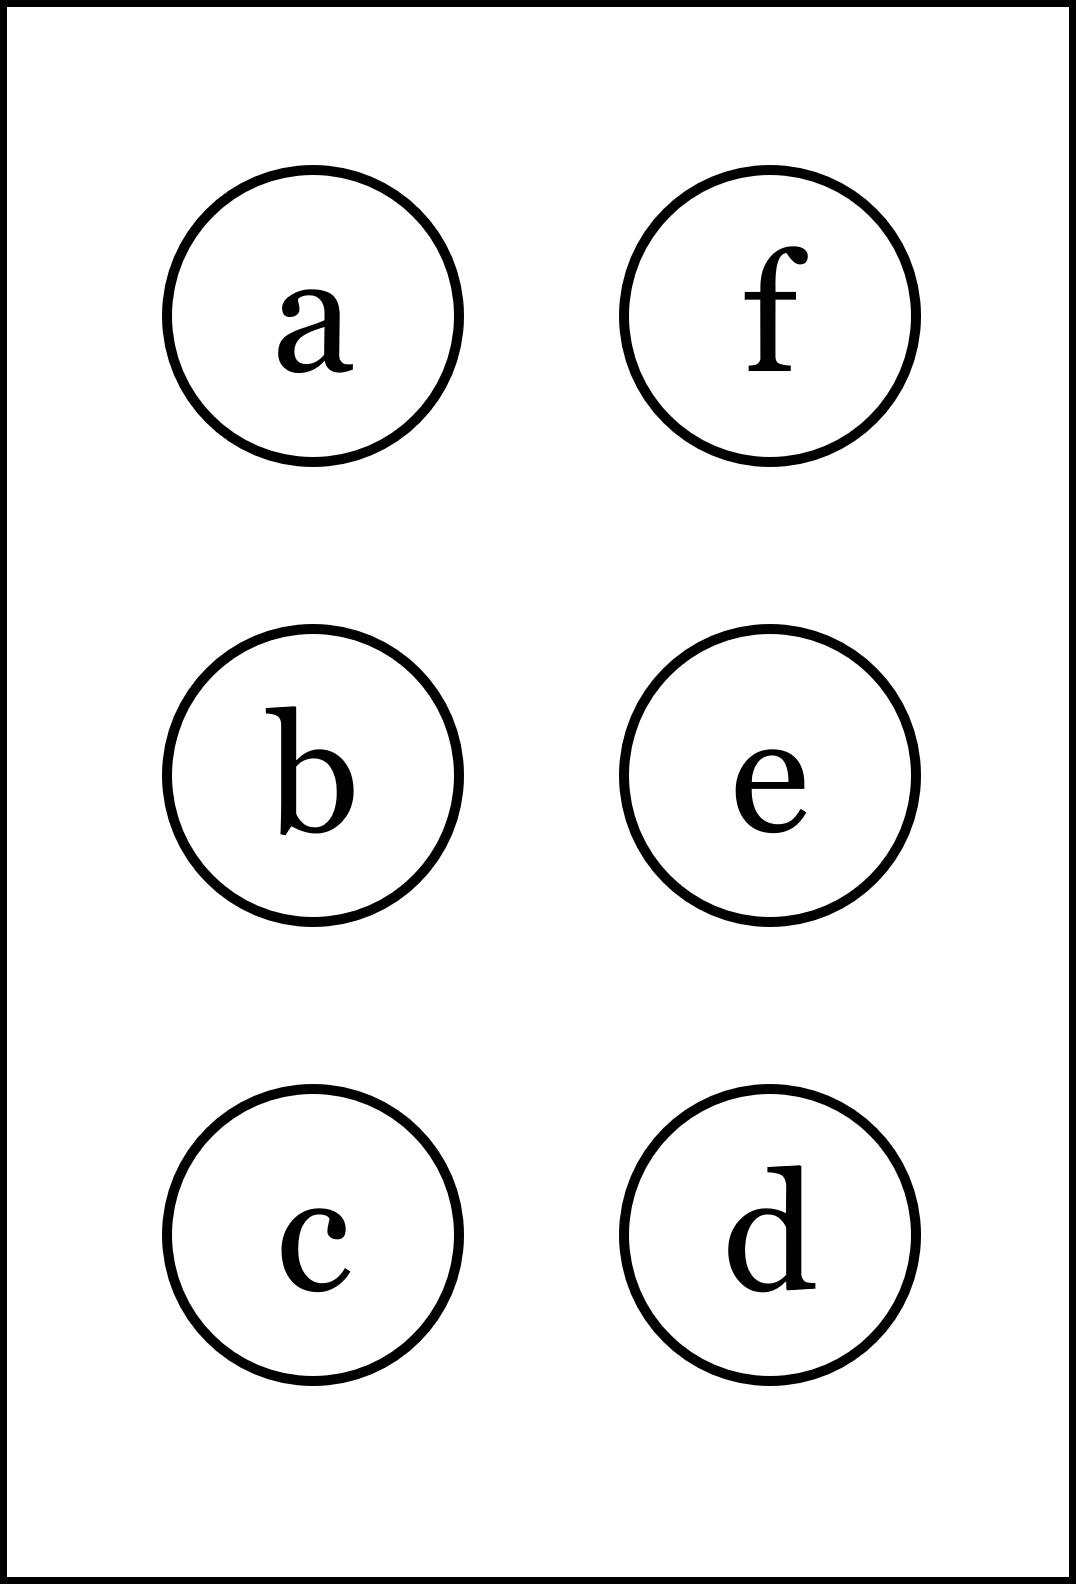
\includegraphics[height=40mm]{../images/braille.png}
{\small Písmeno Braillovej abecedy}
\end{center}
\end{minipage}
\end{center}
\end{minipage}
&
\begin{minipage}[c][104.5mm][t]{0.5\linewidth}
\begin{center}
\vspace{7mm}
{\huge Tečna funkce, skupina \textit{Alpha $\alpha$} -\romannumeral2}\\[5mm]
\textit{Meno:}\phantom{xxxxxxxxxxxxxxxxxxxxxxxxxxxxxxxxxxxxxxxxxxxxxxxxxxxxxxxxxxxxxxxxx}\\[5mm]
\begin{minipage}{0.95\linewidth}
\begin{center}
V \textbf{(a)} a \textbf{(b)} urči \text{rovnicu tečny} $y = kx + q$ ku funkci $f(x)$ v bode $x_0$.\\V \textbf{(c)} a \textbf{(d)} urči ypsilonové souřadnice bodů, ve kterých je sklon $f(x)$ rovný $k$.\\Pokud se výsledky shodujú s těmi za otazníky, tak napravo obarvi\\příslušející kroužek načerno. \textbf{Spolu odevzdejte výsledné slovo}.
\end{center}
\end{minipage}
\\[1mm]
\begin{minipage}{0.79\linewidth}
\begin{center}
\begin{varwidth}{\linewidth}
\begin{enumerate}
\small
\item $f(x)=\cfrac{-8x+2}{x+7}\enspace , \enspace x_0=3$\quad \dotfill\; ???\;\dotfill \quad $y = -\frac{29}{50}x-\frac{23}{50}$
\item $f(x)=6\sqrt{-3x-4}\enspace , \enspace x_0=-\frac{13}{3}$\quad \dotfill\; ???\;\dotfill \quad $y = -3x+10$
\item $f(x)=-5x^2+4x-5\enspace , \enspace k=5$\quad \dotfill\; ???\;\dotfill \quad $-\frac{109}{20}$
\item $f(x)=x^3-6x^2-32x-3\enspace , \enspace k=4$\quad \dotfill\; ???\;\dotfill \quad $29 , 189$
\item \quad \dotfill\; ???\;\dotfill \quad nebarvi
\item \quad \dotfill\; ???\;\dotfill \quad nebarvi
\end{enumerate}
\end{varwidth}
\end{center}
\end{minipage}
\begin{minipage}{0.20\linewidth}
\begin{center}
{\Huge\bfseries 2.} \\[2mm]
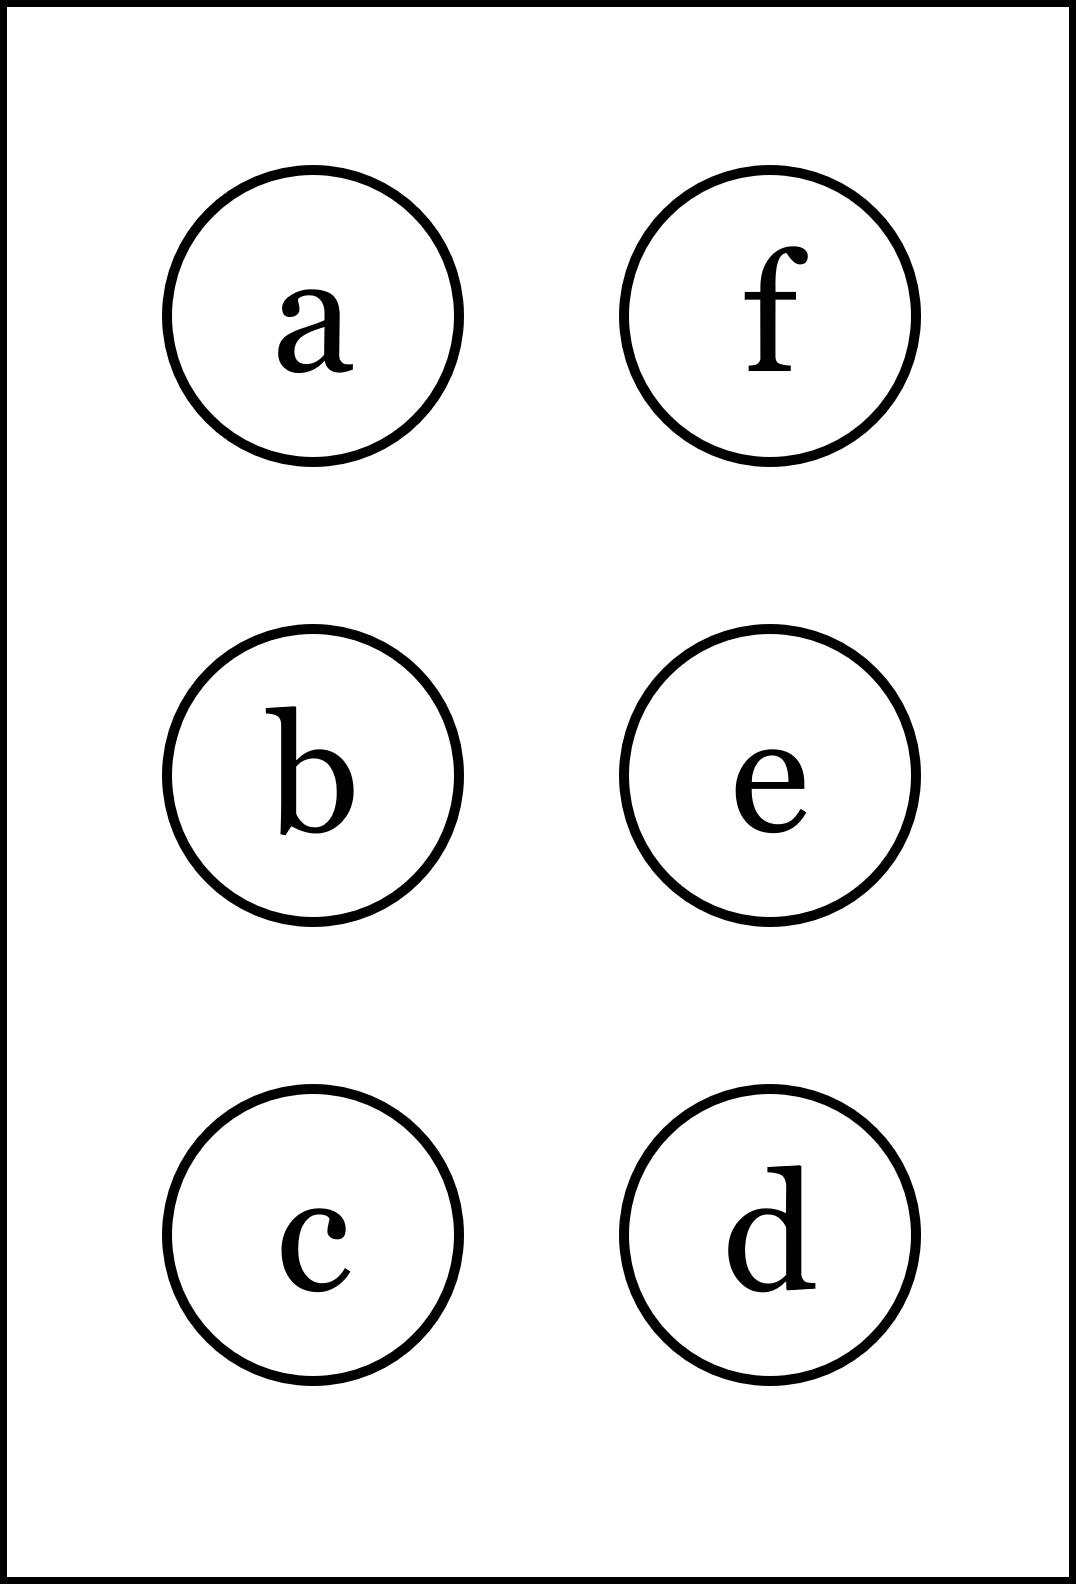
\includegraphics[height=40mm]{../images/braille.png}
{\small Písmeno Braillovej abecedy}
\end{center}
\end{minipage}
\end{center}
\end{minipage}
\\ \hdashline
\begin{minipage}[c][104.5mm][t]{0.5\linewidth}
\begin{center}
\vspace{7mm}
{\huge Tečna funkce, skupina \textit{Alpha $\alpha$} -\romannumeral3}\\[5mm]
\textit{Meno:}\phantom{xxxxxxxxxxxxxxxxxxxxxxxxxxxxxxxxxxxxxxxxxxxxxxxxxxxxxxxxxxxxxxxxx}\\[5mm]
\begin{minipage}{0.95\linewidth}
\begin{center}
V \textbf{(a)} a \textbf{(b)} urči \text{rovnicu tečny} $y = kx + q$ ku funkci $f(x)$ v bode $x_0$.\\V \textbf{(c)} a \textbf{(d)} urči ypsilonové souřadnice bodů, ve kterých je sklon $f(x)$ rovný $k$.\\Pokud se výsledky shodujú s těmi za otazníky, tak napravo obarvi\\příslušející kroužek načerno. \textbf{Spolu odevzdejte výsledné slovo}.
\end{center}
\end{minipage}
\\[1mm]
\begin{minipage}{0.79\linewidth}
\begin{center}
\begin{varwidth}{\linewidth}
\begin{enumerate}
\small
\item $f(x)=\cfrac{-2x-2}{4x-2}\enspace , \enspace x_0=2$\quad \dotfill\; ???\;\dotfill \quad $y = \frac{1}{3}x-\frac{5}{3}$
\item $f(x)=-4\sqrt{3x-9}\enspace , \enspace x_0=\frac{10}{3}$\quad \dotfill\; ???\;\dotfill \quad $y = -6x+32$
\item $f(x)=-6x^2+x-2\enspace , \enspace k=-3$\quad \dotfill\; ???\;\dotfill \quad $-\frac{7}{3}$
\item $f(x)=x^3-9x^2-51x+2\enspace , \enspace k=-3$\quad \dotfill\; ???\;\dotfill \quad $60 , 346$
\item \quad \dotfill\; ???\;\dotfill \quad vybarvi
\item \quad \dotfill\; ???\;\dotfill \quad nebarvi
\end{enumerate}
\end{varwidth}
\end{center}
\end{minipage}
\begin{minipage}{0.20\linewidth}
\begin{center}
{\Huge\bfseries 3.} \\[2mm]
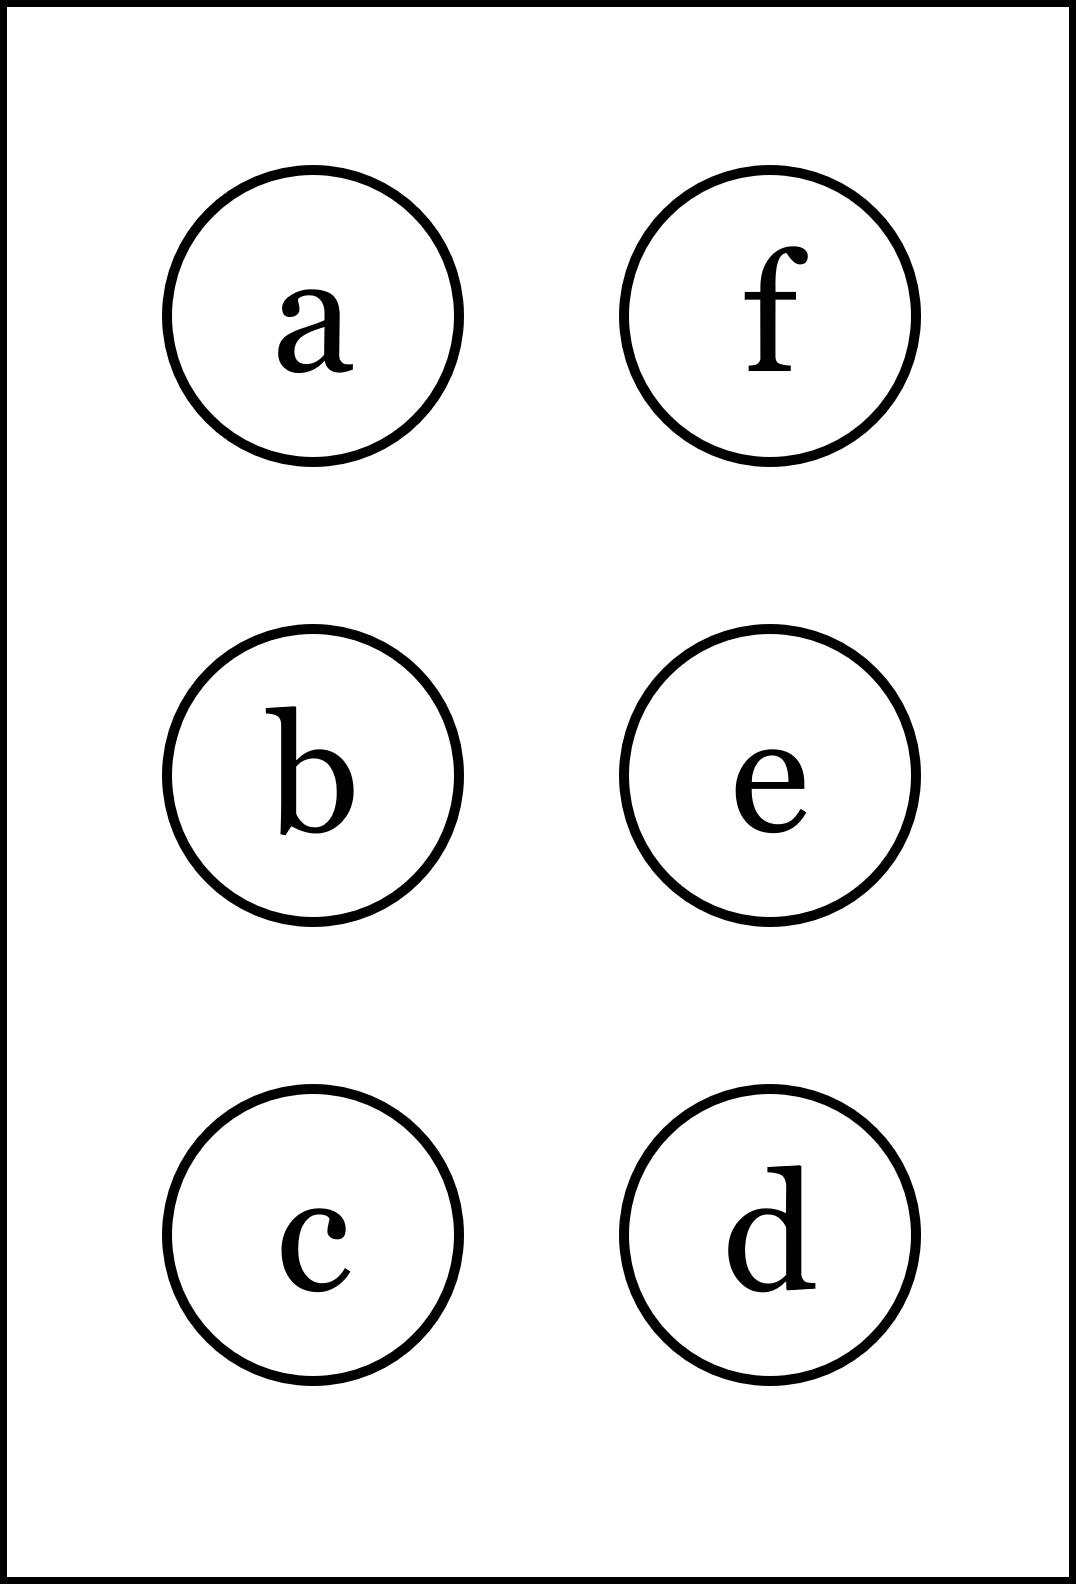
\includegraphics[height=40mm]{../images/braille.png}
{\small Písmeno Braillovej abecedy}
\end{center}
\end{minipage}
\end{center}
\end{minipage}
&
\begin{minipage}[c][104.5mm][t]{0.5\linewidth}
\begin{center}
\vspace{7mm}
{\huge Tečna funkce, skupina \textit{Alpha $\alpha$} -\romannumeral4}\\[5mm]
\textit{Meno:}\phantom{xxxxxxxxxxxxxxxxxxxxxxxxxxxxxxxxxxxxxxxxxxxxxxxxxxxxxxxxxxxxxxxxx}\\[5mm]
\begin{minipage}{0.95\linewidth}
\begin{center}
V \textbf{(a)} a \textbf{(b)} urči \text{rovnicu tečny} $y = kx + q$ ku funkci $f(x)$ v bode $x_0$.\\V \textbf{(c)} a \textbf{(d)} urči ypsilonové souřadnice bodů, ve kterých je sklon $f(x)$ rovný $k$.\\Pokud se výsledky shodujú s těmi za otazníky, tak napravo obarvi\\příslušející kroužek načerno. \textbf{Spolu odevzdejte výsledné slovo}.
\end{center}
\end{minipage}
\\[1mm]
\begin{minipage}{0.79\linewidth}
\begin{center}
\begin{varwidth}{\linewidth}
\begin{enumerate}
\small
\item $f(x)=\cfrac{-4x-3}{2x+3}\enspace , \enspace x_0=-1$\quad \dotfill\; ???\;\dotfill \quad $y = -6x-5$
\item $f(x)=-3\sqrt{-3x-7}\enspace , \enspace x_0=-\frac{8}{3}$\quad \dotfill\; ???\;\dotfill \quad $y = \frac{9}{2}x+9$
\item $f(x)=-4x^2+7x+9\enspace , \enspace k=-9$\quad \dotfill\; ???\;\dotfill \quad $7$
\item $f(x)=x^3-6x^2-68x+2\enspace , \enspace k=-5$\quad \dotfill\; ???\;\dotfill \quad $125 , 527$
\item \quad \dotfill\; ???\;\dotfill \quad nebarvi
\item \quad \dotfill\; ???\;\dotfill \quad nebarvi
\end{enumerate}
\end{varwidth}
\end{center}
\end{minipage}
\begin{minipage}{0.20\linewidth}
\begin{center}
{\Huge\bfseries 4.} \\[2mm]
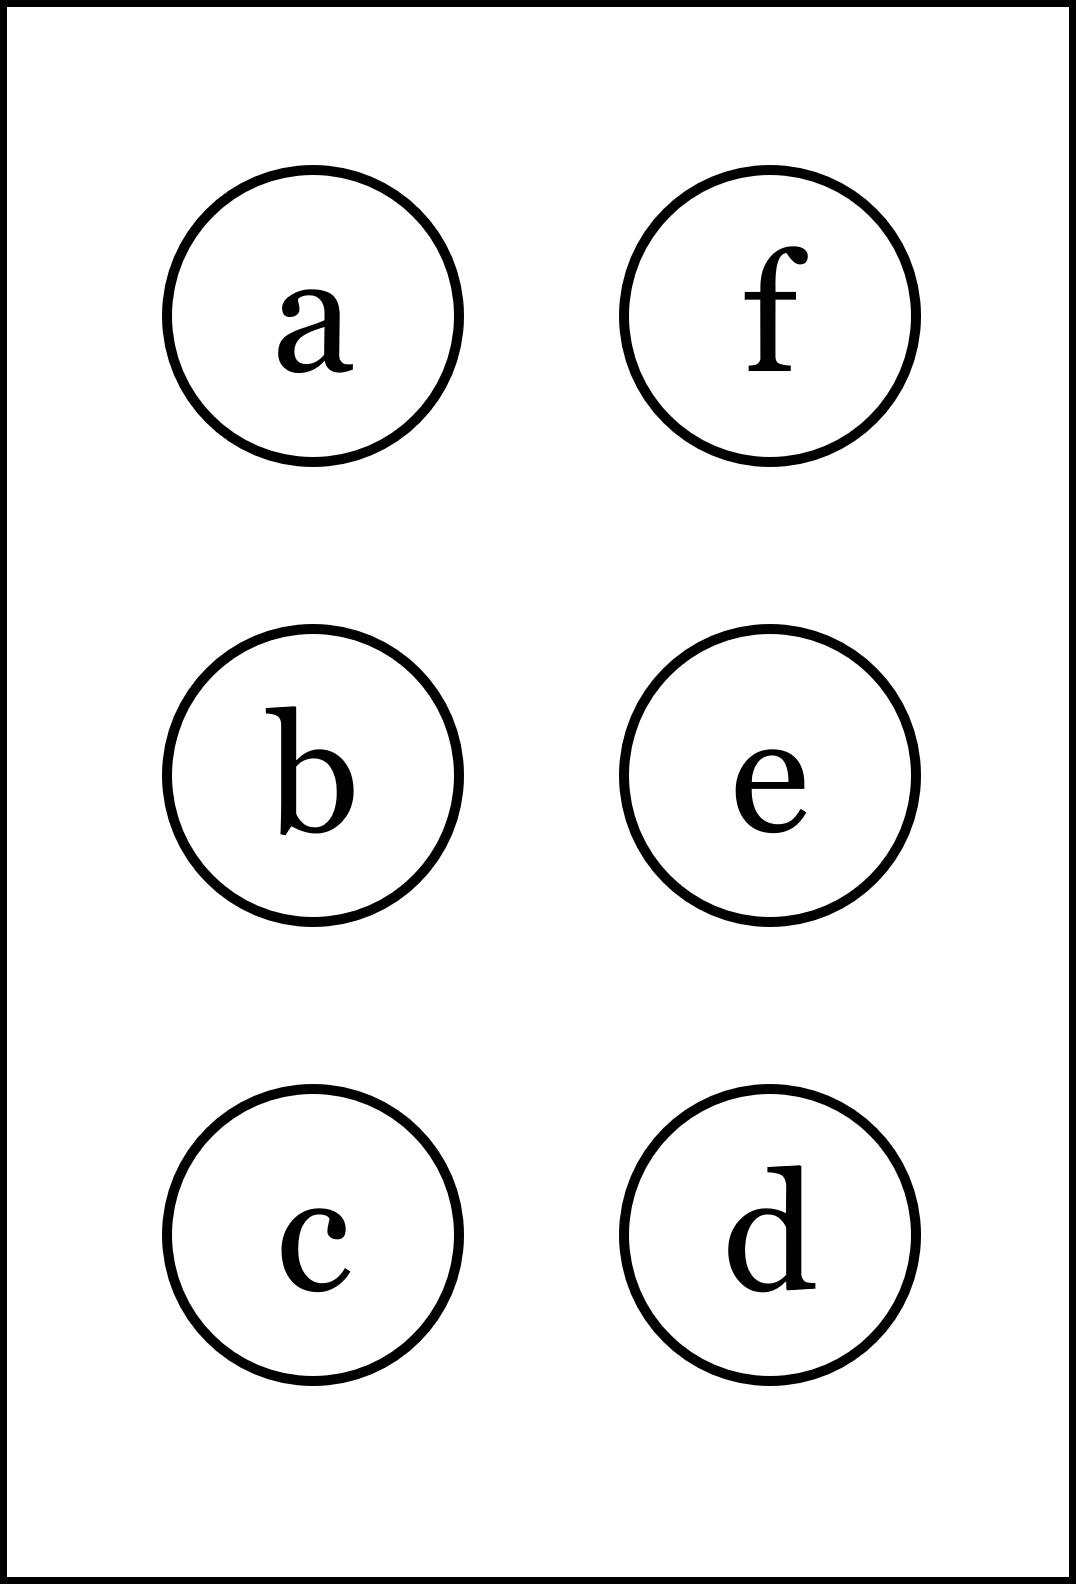
\includegraphics[height=40mm]{../images/braille.png}
{\small Písmeno Braillovej abecedy}
\end{center}
\end{minipage}
\end{center}
\end{minipage}
%
\end{tabular}
\newpage
\thispagestyle{empty}
\begin{tabular}{c:c}
\begin{minipage}[c][104.5mm][t]{0.5\linewidth}
\begin{center}
\vspace{7mm}
{\huge Tečna funkce, skupina \textit{Beta $\beta$} -\romannumeral1}\\[5mm]
\textit{Meno:}\phantom{xxxxxxxxxxxxxxxxxxxxxxxxxxxxxxxxxxxxxxxxxxxxxxxxxxxxxxxxxxxxxxxxx}\\[5mm]
\begin{minipage}{0.95\linewidth}
\begin{center}
V \textbf{(a)} a \textbf{(b)} urči \text{rovnicu tečny} $y = kx + q$ ku funkci $f(x)$ v bode $x_0$.\\V \textbf{(c)} a \textbf{(d)} urči ypsilonové souřadnice bodů, ve kterých je sklon $f(x)$ rovný $k$.\\Pokud se výsledky shodujú s těmi za otazníky, tak napravo obarvi\\příslušející kroužek načerno. \textbf{Spolu odevzdejte výsledné slovo}.
\end{center}
\end{minipage}
\\[1mm]
\begin{minipage}{0.79\linewidth}
\begin{center}
\begin{varwidth}{\linewidth}
\begin{enumerate}
\small
\item $f(x)=\cfrac{2x+7}{9x+1}\enspace , \enspace x_0=1$\quad \dotfill\; ???\;\dotfill \quad $y = -\frac{61}{100}x-\frac{101}{100}$
\item $f(x)=3\sqrt{-4x-3}\enspace , \enspace x_0=-7$\quad \dotfill\; ???\;\dotfill \quad $y = -\frac{6}{5}x+\frac{33}{5}$
\item $f(x)=8x^2+x-1\enspace , \enspace k=-4$\quad \dotfill\; ???\;\dotfill \quad $-\frac{17}{32}$
\item $f(x)=5x^3-15x^2-46x+4\enspace , \enspace k=-1$\quad \dotfill\; ???\;\dotfill \quad $30 , -134$
\item \quad \dotfill\; ???\;\dotfill \quad nebarvi
\item \quad \dotfill\; ???\;\dotfill \quad vybarvi
\end{enumerate}
\end{varwidth}
\end{center}
\end{minipage}
\begin{minipage}{0.20\linewidth}
\begin{center}
{\Huge\bfseries 1.} \\[2mm]
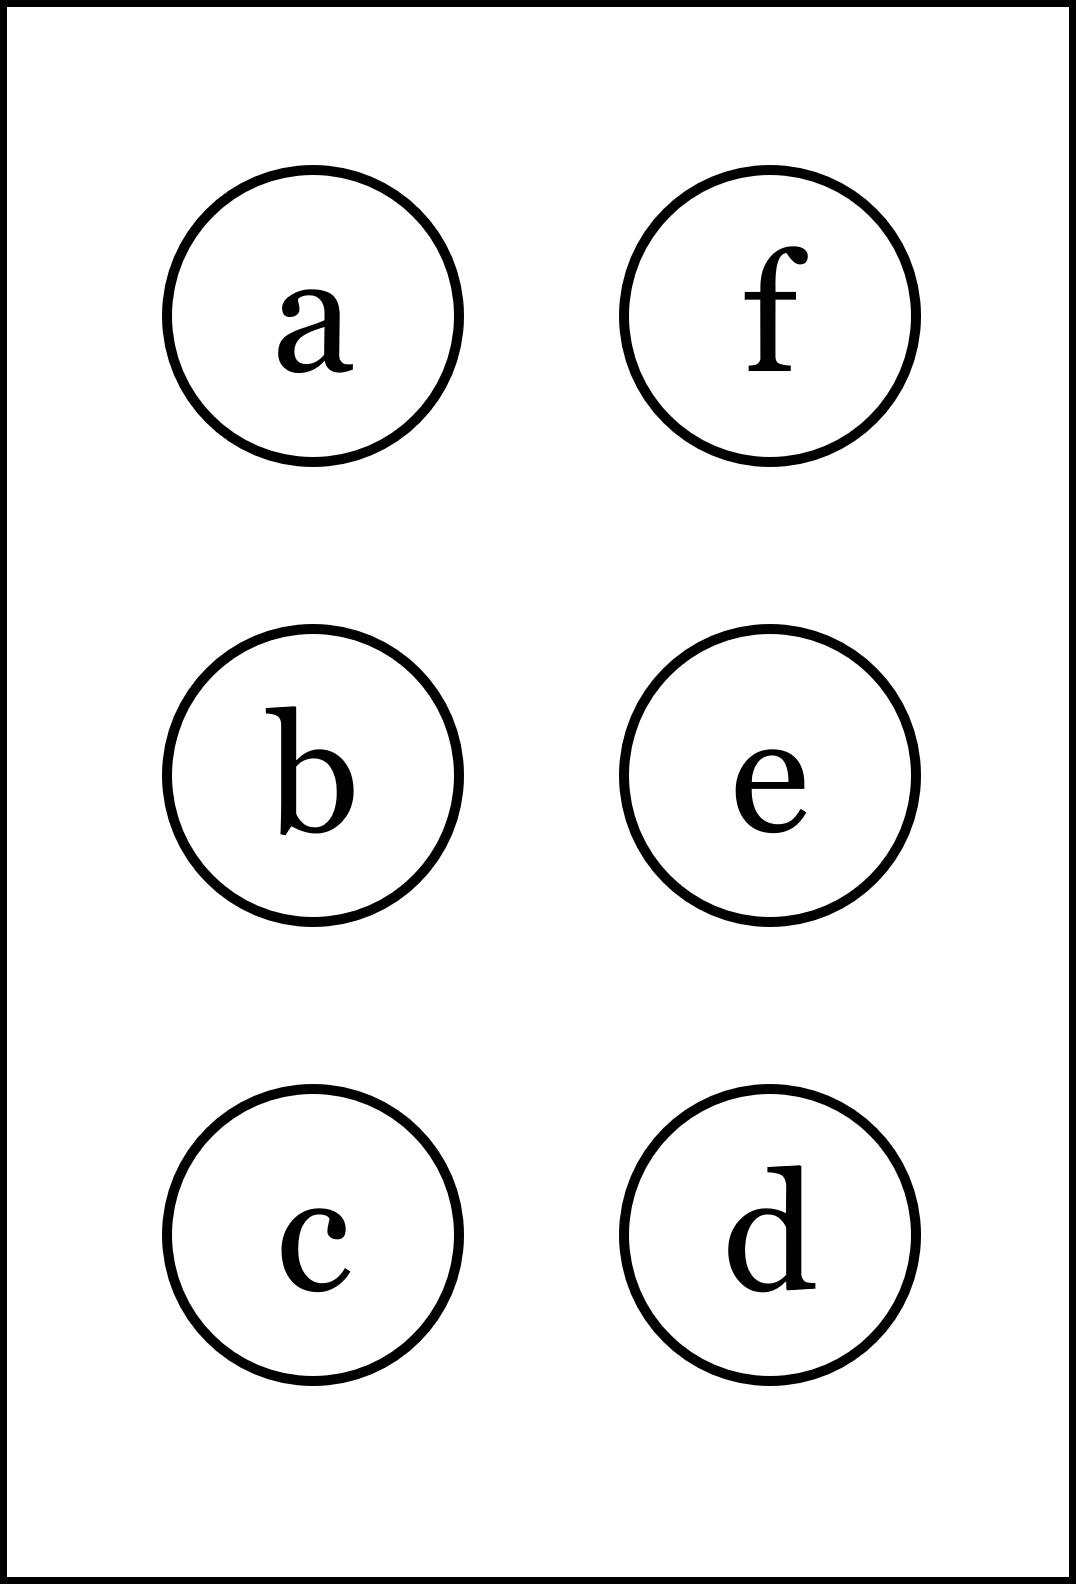
\includegraphics[height=40mm]{../images/braille.png}
{\small Písmeno Braillovej abecedy}
\end{center}
\end{minipage}
\end{center}
\end{minipage}
&
\begin{minipage}[c][104.5mm][t]{0.5\linewidth}
\begin{center}
\vspace{7mm}
{\huge Tečna funkce, skupina \textit{Beta $\beta$} -\romannumeral2}\\[5mm]
\textit{Meno:}\phantom{xxxxxxxxxxxxxxxxxxxxxxxxxxxxxxxxxxxxxxxxxxxxxxxxxxxxxxxxxxxxxxxxx}\\[5mm]
\begin{minipage}{0.95\linewidth}
\begin{center}
V \textbf{(a)} a \textbf{(b)} urči \text{rovnicu tečny} $y = kx + q$ ku funkci $f(x)$ v bode $x_0$.\\V \textbf{(c)} a \textbf{(d)} urči ypsilonové souřadnice bodů, ve kterých je sklon $f(x)$ rovný $k$.\\Pokud se výsledky shodujú s těmi za otazníky, tak napravo obarvi\\příslušející kroužek načerno. \textbf{Spolu odevzdejte výsledné slovo}.
\end{center}
\end{minipage}
\\[1mm]
\begin{minipage}{0.79\linewidth}
\begin{center}
\begin{varwidth}{\linewidth}
\begin{enumerate}
\small
\item $f(x)=\cfrac{6x+4}{2x-2}\enspace , \enspace x_0=2$\quad \dotfill\; ???\;\dotfill \quad $y = -5x+2$
\item $f(x)=3\sqrt{-4x+9}\enspace , \enspace x_0=0$\quad \dotfill\; ???\;\dotfill \quad $y = -2x+9$
\item $f(x)=-2x^2-3x+2\enspace , \enspace k=2$\quad \dotfill\; ???\;\dotfill \quad $-\frac{11}{8}$
\item $f(x)=5x^3-15x^2-48x-2\enspace , \enspace k=-3$\quad \dotfill\; ???\;\dotfill \quad $26 , 142$
\item \quad \dotfill\; ???\;\dotfill \quad nebarvi
\item \quad \dotfill\; ???\;\dotfill \quad vybarvi
\end{enumerate}
\end{varwidth}
\end{center}
\end{minipage}
\begin{minipage}{0.20\linewidth}
\begin{center}
{\Huge\bfseries 2.} \\[2mm]
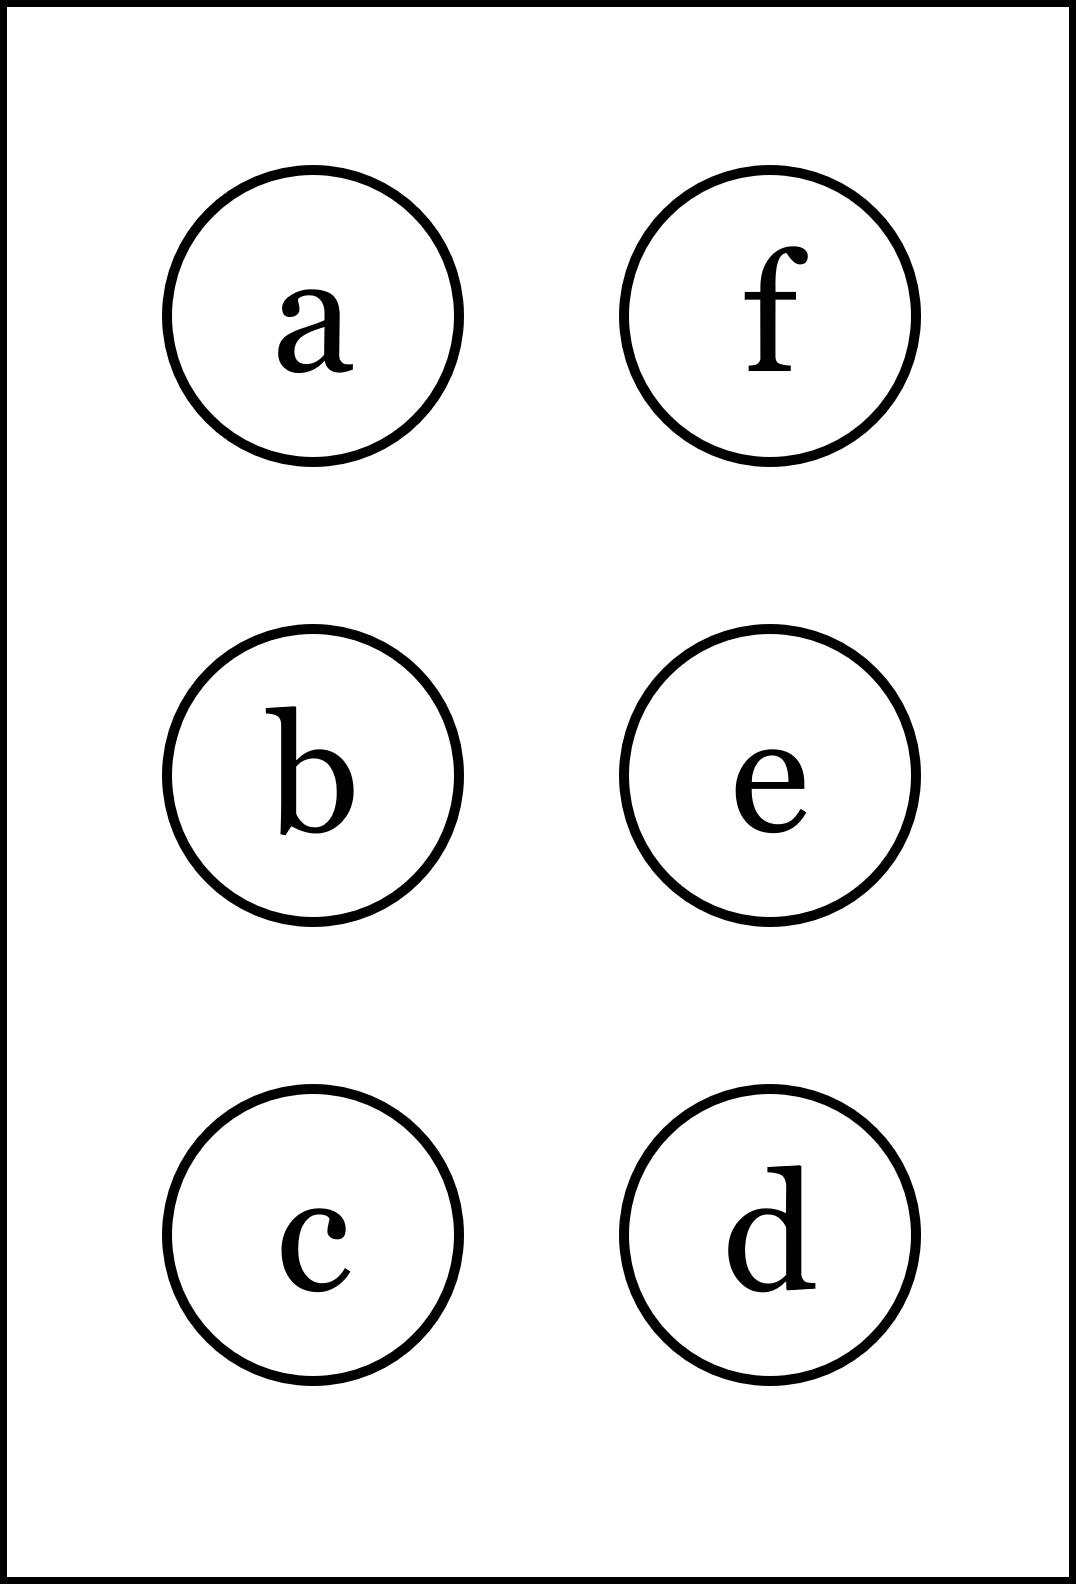
\includegraphics[height=40mm]{../images/braille.png}
{\small Písmeno Braillovej abecedy}
\end{center}
\end{minipage}
\end{center}
\end{minipage}
\\ \hdashline
\begin{minipage}[c][104.5mm][t]{0.5\linewidth}
\begin{center}
\vspace{7mm}
{\huge Tečna funkce, skupina \textit{Beta $\beta$} -\romannumeral3}\\[5mm]
\textit{Meno:}\phantom{xxxxxxxxxxxxxxxxxxxxxxxxxxxxxxxxxxxxxxxxxxxxxxxxxxxxxxxxxxxxxxxxx}\\[5mm]
\begin{minipage}{0.95\linewidth}
\begin{center}
V \textbf{(a)} a \textbf{(b)} urči \text{rovnicu tečny} $y = kx + q$ ku funkci $f(x)$ v bode $x_0$.\\V \textbf{(c)} a \textbf{(d)} urči ypsilonové souřadnice bodů, ve kterých je sklon $f(x)$ rovný $k$.\\Pokud se výsledky shodujú s těmi za otazníky, tak napravo obarvi\\příslušející kroužek načerno. \textbf{Spolu odevzdejte výsledné slovo}.
\end{center}
\end{minipage}
\\[1mm]
\begin{minipage}{0.79\linewidth}
\begin{center}
\begin{varwidth}{\linewidth}
\begin{enumerate}
\small
\item $f(x)=\cfrac{-8x+4}{2x+2}\enspace , \enspace x_0=-2$\quad \dotfill\; ???\;\dotfill \quad $y = -6x-6$
\item $f(x)=\sqrt{7x-3}\enspace , \enspace x_0=\frac{12}{7}$\quad \dotfill\; ???\;\dotfill \quad $y = \frac{7}{6}x+1$
\item $f(x)=3x^2+2x+1\enspace , \enspace k=5$\quad \dotfill\; ???\;\dotfill \quad $\frac{11}{4}$
\item $f(x)=x^3-3x^2-43x-2\enspace , \enspace k=2$\quad \dotfill\; ???\;\dotfill \quad $73 , 263$
\item \quad \dotfill\; ???\;\dotfill \quad vybarvi
\item \quad \dotfill\; ???\;\dotfill \quad vybarvi
\end{enumerate}
\end{varwidth}
\end{center}
\end{minipage}
\begin{minipage}{0.20\linewidth}
\begin{center}
{\Huge\bfseries 3.} \\[2mm]
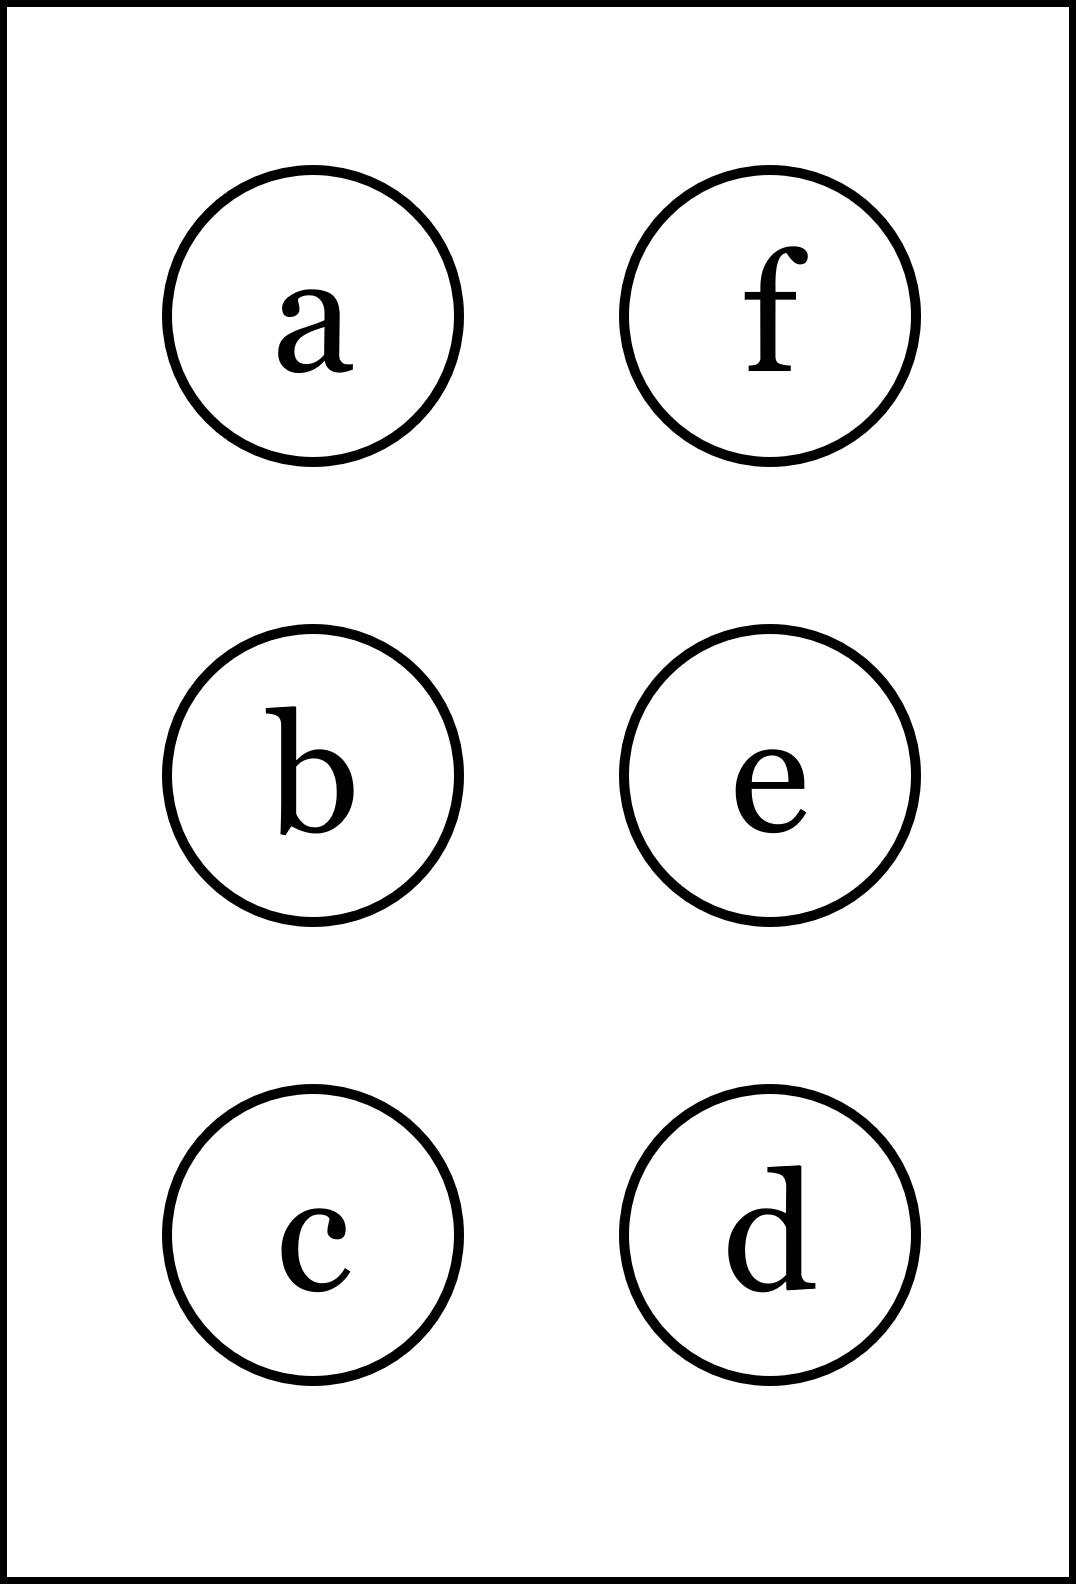
\includegraphics[height=40mm]{../images/braille.png}
{\small Písmeno Braillovej abecedy}
\end{center}
\end{minipage}
\end{center}
\end{minipage}
&
\begin{minipage}[c][104.5mm][t]{0.5\linewidth}
\begin{center}
\vspace{7mm}
{\huge Tečna funkce, skupina \textit{Beta $\beta$} -\romannumeral4}\\[5mm]
\textit{Meno:}\phantom{xxxxxxxxxxxxxxxxxxxxxxxxxxxxxxxxxxxxxxxxxxxxxxxxxxxxxxxxxxxxxxxxx}\\[5mm]
\begin{minipage}{0.95\linewidth}
\begin{center}
V \textbf{(a)} a \textbf{(b)} urči \text{rovnicu tečny} $y = kx + q$ ku funkci $f(x)$ v bode $x_0$.\\V \textbf{(c)} a \textbf{(d)} urči ypsilonové souřadnice bodů, ve kterých je sklon $f(x)$ rovný $k$.\\Pokud se výsledky shodujú s těmi za otazníky, tak napravo obarvi\\příslušející kroužek načerno. \textbf{Spolu odevzdejte výsledné slovo}.
\end{center}
\end{minipage}
\\[1mm]
\begin{minipage}{0.79\linewidth}
\begin{center}
\begin{varwidth}{\linewidth}
\begin{enumerate}
\small
\item $f(x)=\cfrac{-4x-5}{5x-1}\enspace , \enspace x_0=2$\quad \dotfill\; ???\;\dotfill \quad $y = \frac{29}{81}x-\frac{175}{81}$
\item $f(x)=-8\sqrt{-3x+1}\enspace , \enspace x_0=-\frac{8}{3}$\quad \dotfill\; ???\;\dotfill \quad $y = 4x-\frac{80}{3}$
\item $f(x)=-6x^2+x-1\enspace , \enspace k=4$\quad \dotfill\; ???\;\dotfill \quad $-\frac{13}{8}$
\item $f(x)=x^3-3x^2-20x-3\enspace , \enspace k=4$\quad \dotfill\; ???\;\dotfill \quad $17 , 93$
\item \quad \dotfill\; ???\;\dotfill \quad vybarvi
\item \quad \dotfill\; ???\;\dotfill \quad nebarvi
\end{enumerate}
\end{varwidth}
\end{center}
\end{minipage}
\begin{minipage}{0.20\linewidth}
\begin{center}
{\Huge\bfseries 4.} \\[2mm]
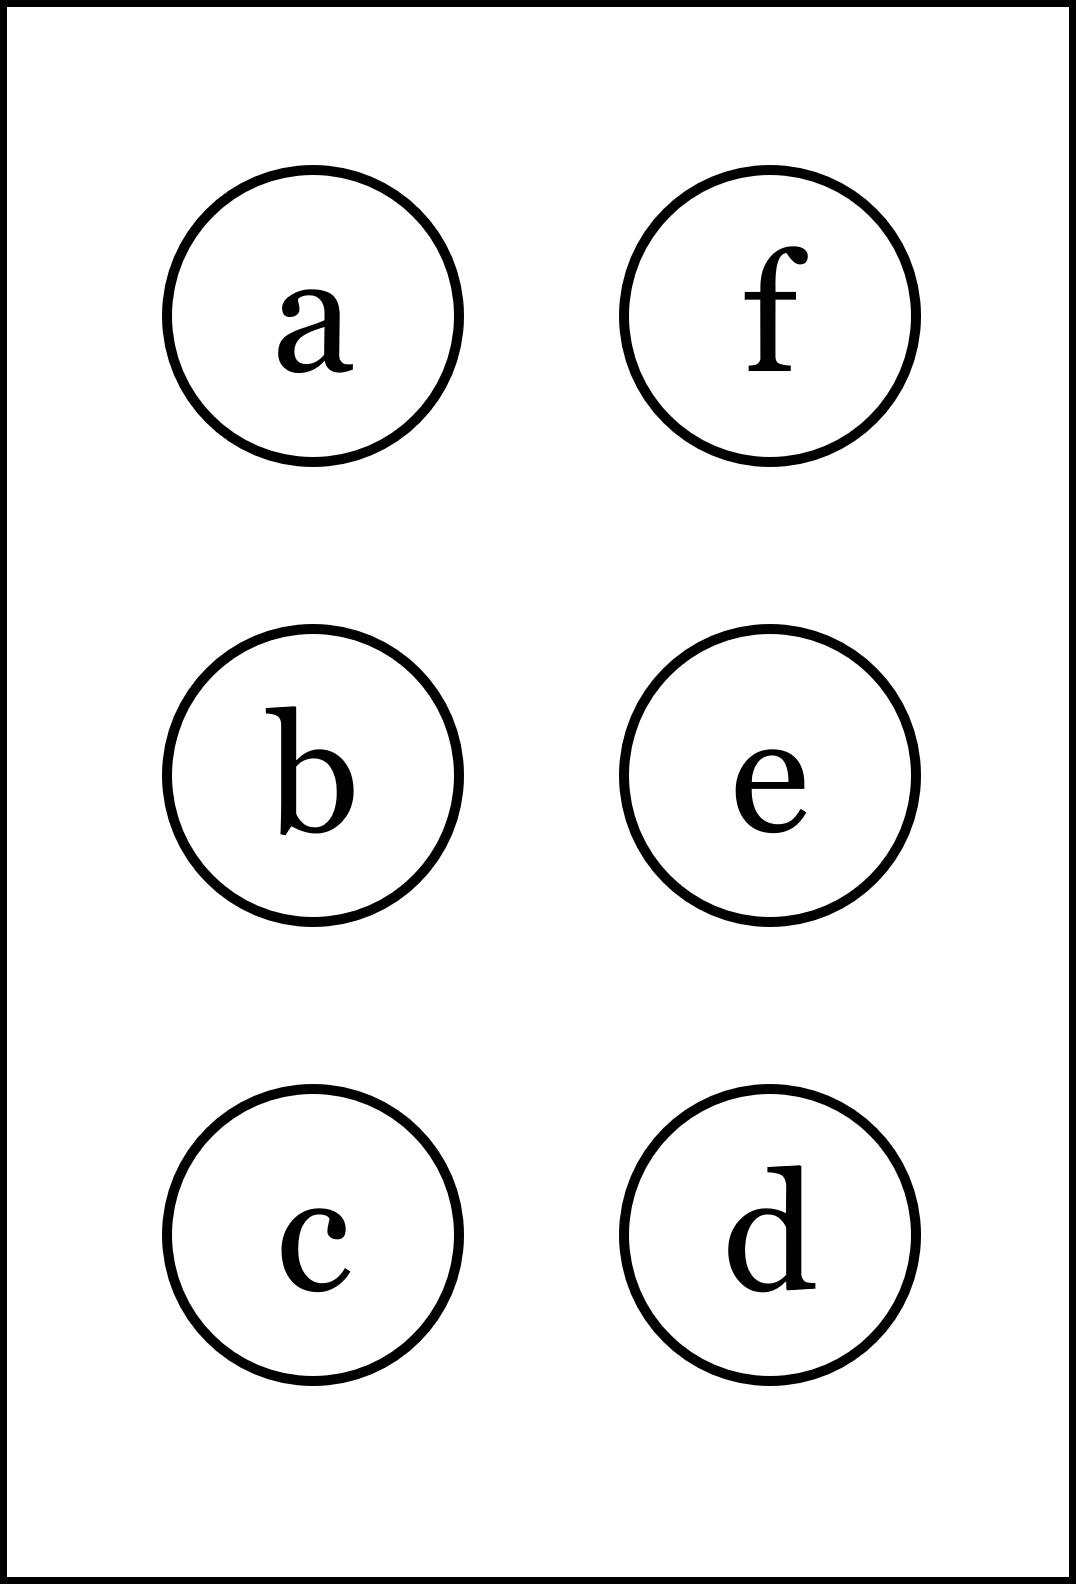
\includegraphics[height=40mm]{../images/braille.png}
{\small Písmeno Braillovej abecedy}
\end{center}
\end{minipage}
\end{center}
\end{minipage}
%
\end{tabular}
\newpage
\thispagestyle{empty}
\begin{tabular}{c:c}
\begin{minipage}[c][104.5mm][t]{0.5\linewidth}
\begin{center}
\vspace{7mm}
{\huge Tečna funkce, skupina \textit{Gamma $\gamma$} -\romannumeral1}\\[5mm]
\textit{Meno:}\phantom{xxxxxxxxxxxxxxxxxxxxxxxxxxxxxxxxxxxxxxxxxxxxxxxxxxxxxxxxxxxxxxxxx}\\[5mm]
\begin{minipage}{0.95\linewidth}
\begin{center}
V \textbf{(a)} a \textbf{(b)} urči \text{rovnicu tečny} $y = kx + q$ ku funkci $f(x)$ v bode $x_0$.\\V \textbf{(c)} a \textbf{(d)} urči ypsilonové souřadnice bodů, ve kterých je sklon $f(x)$ rovný $k$.\\Pokud se výsledky shodujú s těmi za otazníky, tak napravo obarvi\\příslušející kroužek načerno. \textbf{Spolu odevzdejte výsledné slovo}.
\end{center}
\end{minipage}
\\[1mm]
\begin{minipage}{0.79\linewidth}
\begin{center}
\begin{varwidth}{\linewidth}
\begin{enumerate}
\small
\item $f(x)=\cfrac{-9x+4}{7x-4}\enspace , \enspace x_0=-1$\quad \dotfill\; ???\;\dotfill \quad $y = \frac{8}{121}x-\frac{135}{121}$
\item $f(x)=-2\sqrt{6x-3}\enspace , \enspace x_0=\frac{7}{6}$\quad \dotfill\; ???\;\dotfill \quad $y = -3x-\frac{1}{2}$
\item $f(x)=x^2+7x+3\enspace , \enspace k=-2$\quad \dotfill\; ???\;\dotfill \quad $-\frac{57}{4}$
\item $f(x)=3x^3-18x^2-105x-2\enspace , \enspace k=3$\quad \dotfill\; ???\;\dotfill \quad $112 , 628$
\item \quad \dotfill\; ???\;\dotfill \quad vybarvi
\item \quad \dotfill\; ???\;\dotfill \quad nebarvi
\end{enumerate}
\end{varwidth}
\end{center}
\end{minipage}
\begin{minipage}{0.20\linewidth}
\begin{center}
{\Huge\bfseries 1.} \\[2mm]
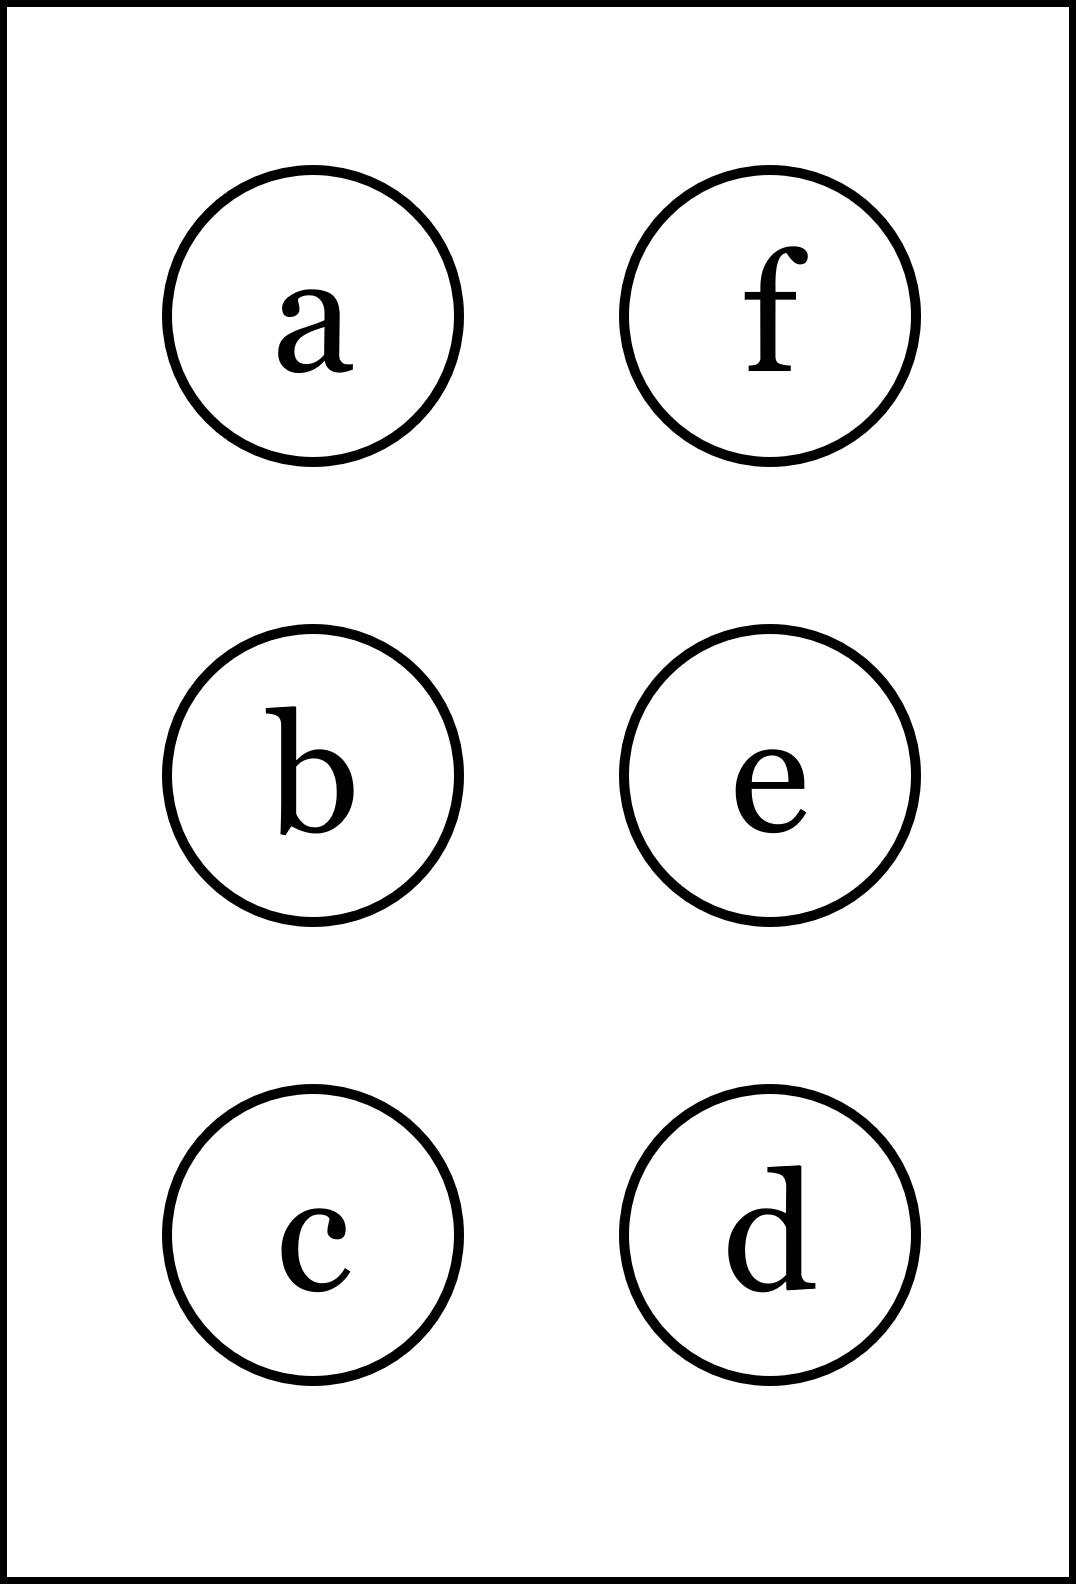
\includegraphics[height=40mm]{../images/braille.png}
{\small Písmeno Braillovej abecedy}
\end{center}
\end{minipage}
\end{center}
\end{minipage}
&
\begin{minipage}[c][104.5mm][t]{0.5\linewidth}
\begin{center}
\vspace{7mm}
{\huge Tečna funkce, skupina \textit{Gamma $\gamma$} -\romannumeral2}\\[5mm]
\textit{Meno:}\phantom{xxxxxxxxxxxxxxxxxxxxxxxxxxxxxxxxxxxxxxxxxxxxxxxxxxxxxxxxxxxxxxxxx}\\[5mm]
\begin{minipage}{0.95\linewidth}
\begin{center}
V \textbf{(a)} a \textbf{(b)} urči \text{rovnicu tečny} $y = kx + q$ ku funkci $f(x)$ v bode $x_0$.\\V \textbf{(c)} a \textbf{(d)} urči ypsilonové souřadnice bodů, ve kterých je sklon $f(x)$ rovný $k$.\\Pokud se výsledky shodujú s těmi za otazníky, tak napravo obarvi\\příslušející kroužek načerno. \textbf{Spolu odevzdejte výsledné slovo}.
\end{center}
\end{minipage}
\\[1mm]
\begin{minipage}{0.79\linewidth}
\begin{center}
\begin{varwidth}{\linewidth}
\begin{enumerate}
\small
\item $f(x)=\cfrac{-6x-2}{x+7}\enspace , \enspace x_0=1$\quad \dotfill\; ???\;\dotfill \quad $y = -\frac{5}{8}x-\frac{3}{8}$
\item $f(x)=4\sqrt{6x-3}\enspace , \enspace x_0=\frac{7}{6}$\quad \dotfill\; ???\;\dotfill \quad $y = 6x+1$
\item $f(x)=3x^2-2x+2\enspace , \enspace k=5$\quad \dotfill\; ???\;\dotfill \quad $\frac{15}{4}$
\item $f(x)=2x^3-12x^2+23x-2\enspace , \enspace k=5$\quad \dotfill\; ???\;\dotfill \quad $11 , -125$
\item \quad \dotfill\; ???\;\dotfill \quad vybarvi
\item \quad \dotfill\; ???\;\dotfill \quad nebarvi
\end{enumerate}
\end{varwidth}
\end{center}
\end{minipage}
\begin{minipage}{0.20\linewidth}
\begin{center}
{\Huge\bfseries 2.} \\[2mm]
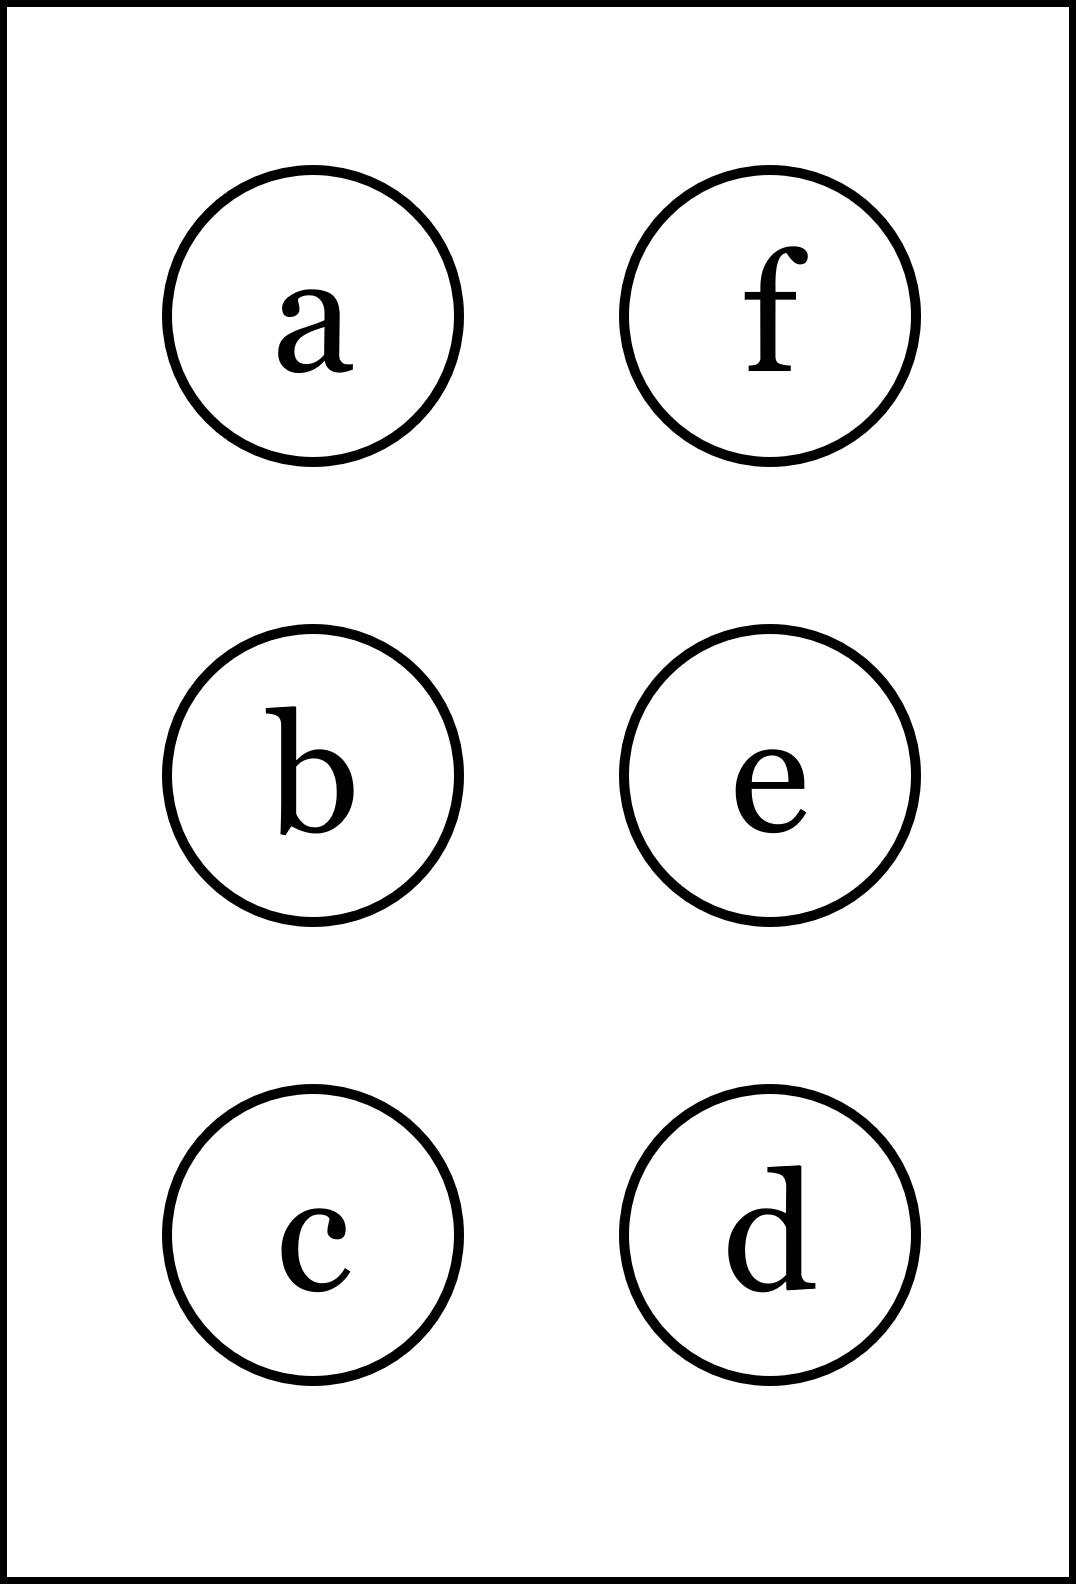
\includegraphics[height=40mm]{../images/braille.png}
{\small Písmeno Braillovej abecedy}
\end{center}
\end{minipage}
\end{center}
\end{minipage}
\\ \hdashline
\begin{minipage}[c][104.5mm][t]{0.5\linewidth}
\begin{center}
\vspace{7mm}
{\huge Tečna funkce, skupina \textit{Gamma $\gamma$} -\romannumeral3}\\[5mm]
\textit{Meno:}\phantom{xxxxxxxxxxxxxxxxxxxxxxxxxxxxxxxxxxxxxxxxxxxxxxxxxxxxxxxxxxxxxxxxx}\\[5mm]
\begin{minipage}{0.95\linewidth}
\begin{center}
V \textbf{(a)} a \textbf{(b)} urči \text{rovnicu tečny} $y = kx + q$ ku funkci $f(x)$ v bode $x_0$.\\V \textbf{(c)} a \textbf{(d)} urči ypsilonové souřadnice bodů, ve kterých je sklon $f(x)$ rovný $k$.\\Pokud se výsledky shodujú s těmi za otazníky, tak napravo obarvi\\příslušející kroužek načerno. \textbf{Spolu odevzdejte výsledné slovo}.
\end{center}
\end{minipage}
\\[1mm]
\begin{minipage}{0.79\linewidth}
\begin{center}
\begin{varwidth}{\linewidth}
\begin{enumerate}
\small
\item $f(x)=\cfrac{6x-3}{x-3}\enspace , \enspace x_0=-3$\quad \dotfill\; ???\;\dotfill \quad $y = -\frac{5}{12}x+\frac{9}{4}$
\item $f(x)=5\sqrt{2x-1}\enspace , \enspace x_0=\frac{5}{2}$\quad \dotfill\; ???\;\dotfill \quad $y = \frac{5}{2}x+\frac{15}{2}$
\item $f(x)=5x^2-9x-7\enspace , \enspace k=2$\quad \dotfill\; ???\;\dotfill \quad $\frac{63}{20}$
\item $f(x)=2x^3-12x^2+16x-2\enspace , \enspace k=-2$\quad \dotfill\; ???\;\dotfill \quad $4 , -104$
\item \quad \dotfill\; ???\;\dotfill \quad nebarvi
\item \quad \dotfill\; ???\;\dotfill \quad nebarvi
\end{enumerate}
\end{varwidth}
\end{center}
\end{minipage}
\begin{minipage}{0.20\linewidth}
\begin{center}
{\Huge\bfseries 3.} \\[2mm]
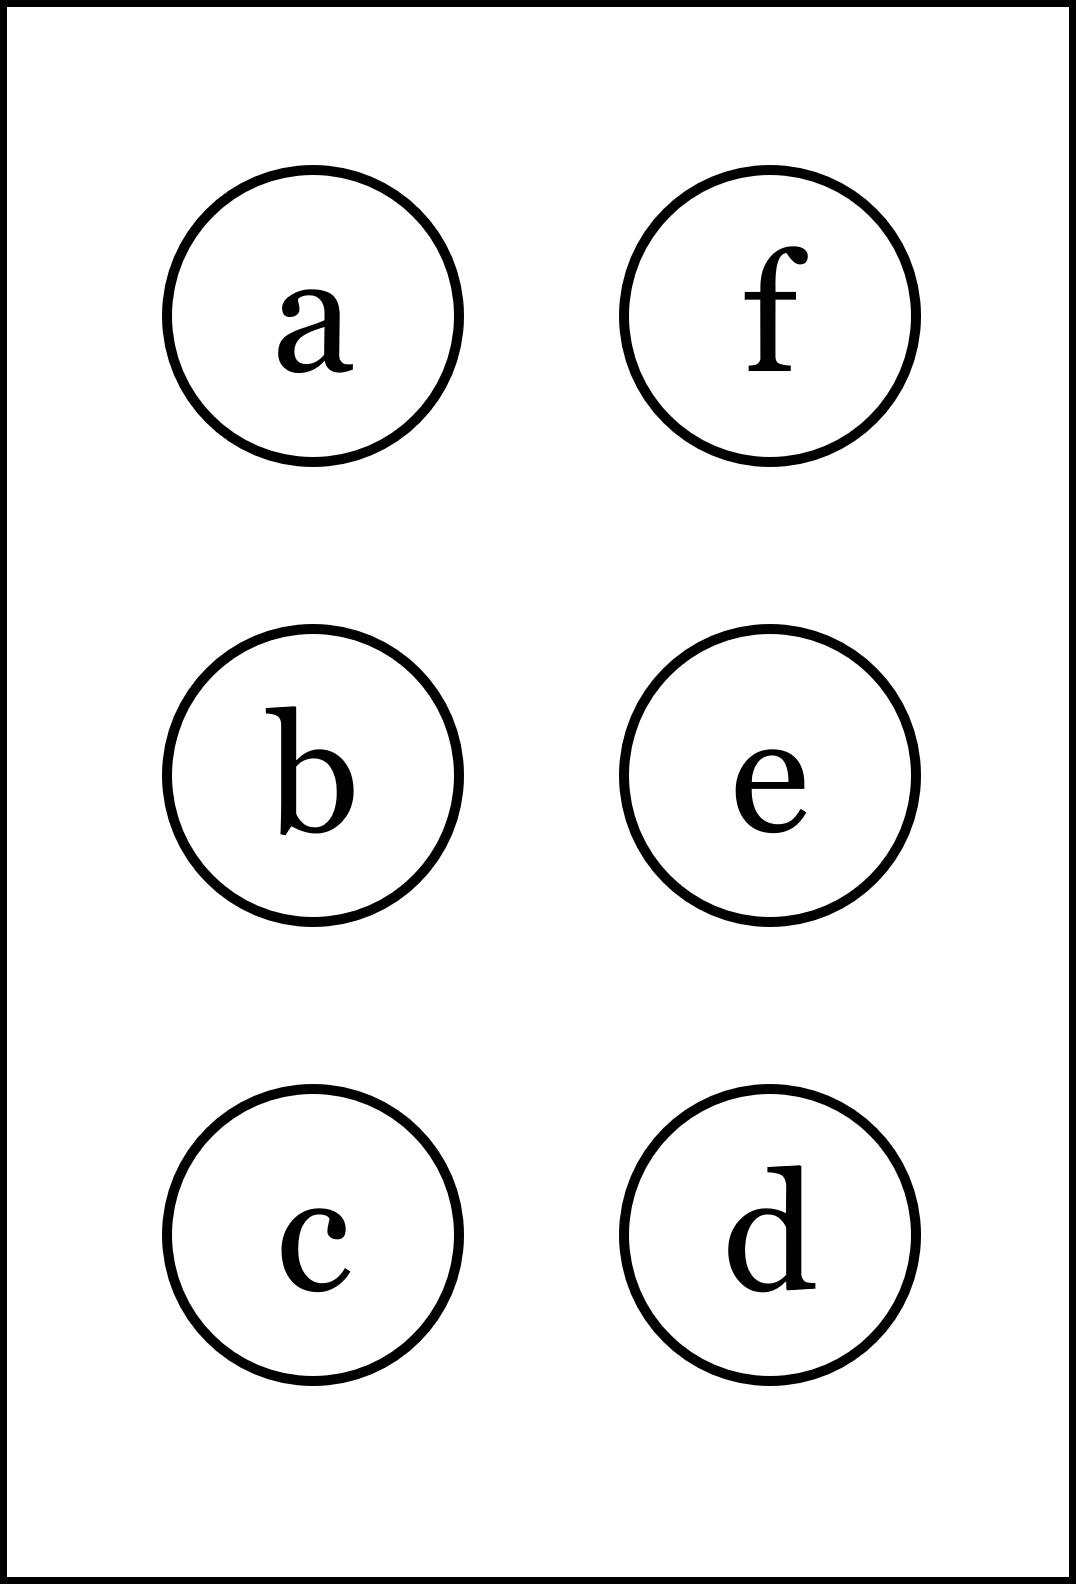
\includegraphics[height=40mm]{../images/braille.png}
{\small Písmeno Braillovej abecedy}
\end{center}
\end{minipage}
\end{center}
\end{minipage}
&
\begin{minipage}[c][104.5mm][t]{0.5\linewidth}
\begin{center}
\vspace{7mm}
{\huge Tečna funkce, skupina \textit{Gamma $\gamma$} -\romannumeral4}\\[5mm]
\textit{Meno:}\phantom{xxxxxxxxxxxxxxxxxxxxxxxxxxxxxxxxxxxxxxxxxxxxxxxxxxxxxxxxxxxxxxxxx}\\[5mm]
\begin{minipage}{0.95\linewidth}
\begin{center}
V \textbf{(a)} a \textbf{(b)} urči \text{rovnicu tečny} $y = kx + q$ ku funkci $f(x)$ v bode $x_0$.\\V \textbf{(c)} a \textbf{(d)} urči ypsilonové souřadnice bodů, ve kterých je sklon $f(x)$ rovný $k$.\\Pokud se výsledky shodujú s těmi za otazníky, tak napravo obarvi\\příslušející kroužek načerno. \textbf{Spolu odevzdejte výsledné slovo}.
\end{center}
\end{minipage}
\\[1mm]
\begin{minipage}{0.79\linewidth}
\begin{center}
\begin{varwidth}{\linewidth}
\begin{enumerate}
\small
\item $f(x)=\cfrac{-4x-2}{5x-3}\enspace , \enspace x_0=2$\quad \dotfill\; ???\;\dotfill \quad $y = \frac{22}{49}x-\frac{114}{49}$
\item $f(x)=\sqrt{8x+7}\enspace , \enspace x_0=\frac{1}{4}$\quad \dotfill\; ???\;\dotfill \quad $y = \frac{4}{3}x+\frac{16}{3}$
\item $f(x)=x^2+3x-6\enspace , \enspace k=8$\quad \dotfill\; ???\;\dotfill \quad $\frac{79}{4}$
\item $f(x)=3x^3-18x^2-109x-4\enspace , \enspace k=-1$\quad \dotfill\; ???\;\dotfill \quad $118 , 650$
\item \quad \dotfill\; ???\;\dotfill \quad vybarvi
\item \quad \dotfill\; ???\;\dotfill \quad vybarvi
\end{enumerate}
\end{varwidth}
\end{center}
\end{minipage}
\begin{minipage}{0.20\linewidth}
\begin{center}
{\Huge\bfseries 4.} \\[2mm]
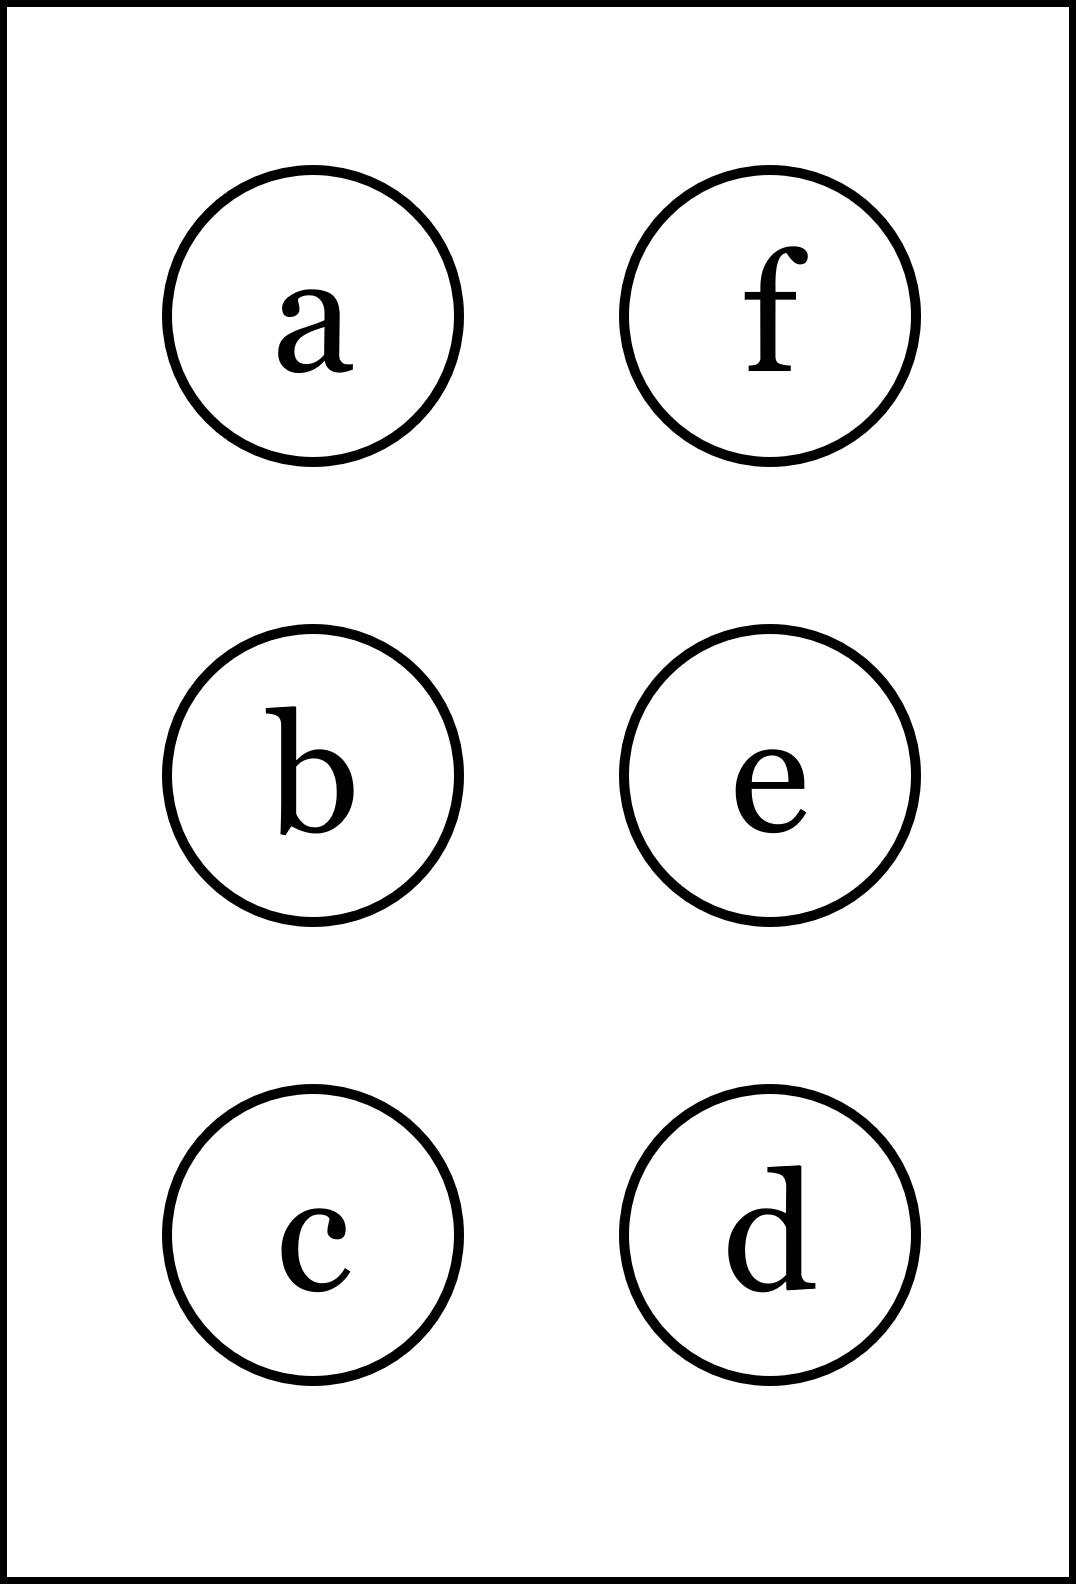
\includegraphics[height=40mm]{../images/braille.png}
{\small Písmeno Braillovej abecedy}
\end{center}
\end{minipage}
\end{center}
\end{minipage}
%
\end{tabular}
\newpage
\thispagestyle{empty}
\begin{tabular}{c:c}
\begin{minipage}[c][104.5mm][t]{0.5\linewidth}
\begin{center}
\vspace{7mm}
{\huge Tečna funkce, skupina \textit{Delta $\delta$} -\romannumeral1}\\[5mm]
\textit{Meno:}\phantom{xxxxxxxxxxxxxxxxxxxxxxxxxxxxxxxxxxxxxxxxxxxxxxxxxxxxxxxxxxxxxxxxx}\\[5mm]
\begin{minipage}{0.95\linewidth}
\begin{center}
V \textbf{(a)} a \textbf{(b)} urči \text{rovnicu tečny} $y = kx + q$ ku funkci $f(x)$ v bode $x_0$.\\V \textbf{(c)} a \textbf{(d)} urči ypsilonové souřadnice bodů, ve kterých je sklon $f(x)$ rovný $k$.\\Pokud se výsledky shodujú s těmi za otazníky, tak napravo obarvi\\příslušející kroužek načerno. \textbf{Spolu odevzdejte výsledné slovo}.
\end{center}
\end{minipage}
\\[1mm]
\begin{minipage}{0.79\linewidth}
\begin{center}
\begin{varwidth}{\linewidth}
\begin{enumerate}
\small
\item $f(x)=\cfrac{2x-5}{-2x+2}\enspace , \enspace x_0=-1$\quad \dotfill\; ???\;\dotfill \quad $y = -\frac{3}{8}x-\frac{17}{8}$
\item $f(x)=2\sqrt{4x-7}\enspace , \enspace x_0=\frac{23}{4}$\quad \dotfill\; ???\;\dotfill \quad $y = x+\frac{9}{4}$
\item $f(x)=-7x^2+2x-4\enspace , \enspace k=5$\quad \dotfill\; ???\;\dotfill \quad $-\frac{19}{4}$
\item $f(x)=3x^3-18x^2-41x+1\enspace , \enspace k=4$\quad \dotfill\; ???\;\dotfill \quad $21 , -279$
\item \quad \dotfill\; ???\;\dotfill \quad nebarvi
\item \quad \dotfill\; ???\;\dotfill \quad nebarvi
\end{enumerate}
\end{varwidth}
\end{center}
\end{minipage}
\begin{minipage}{0.20\linewidth}
\begin{center}
{\Huge\bfseries 1.} \\[2mm]
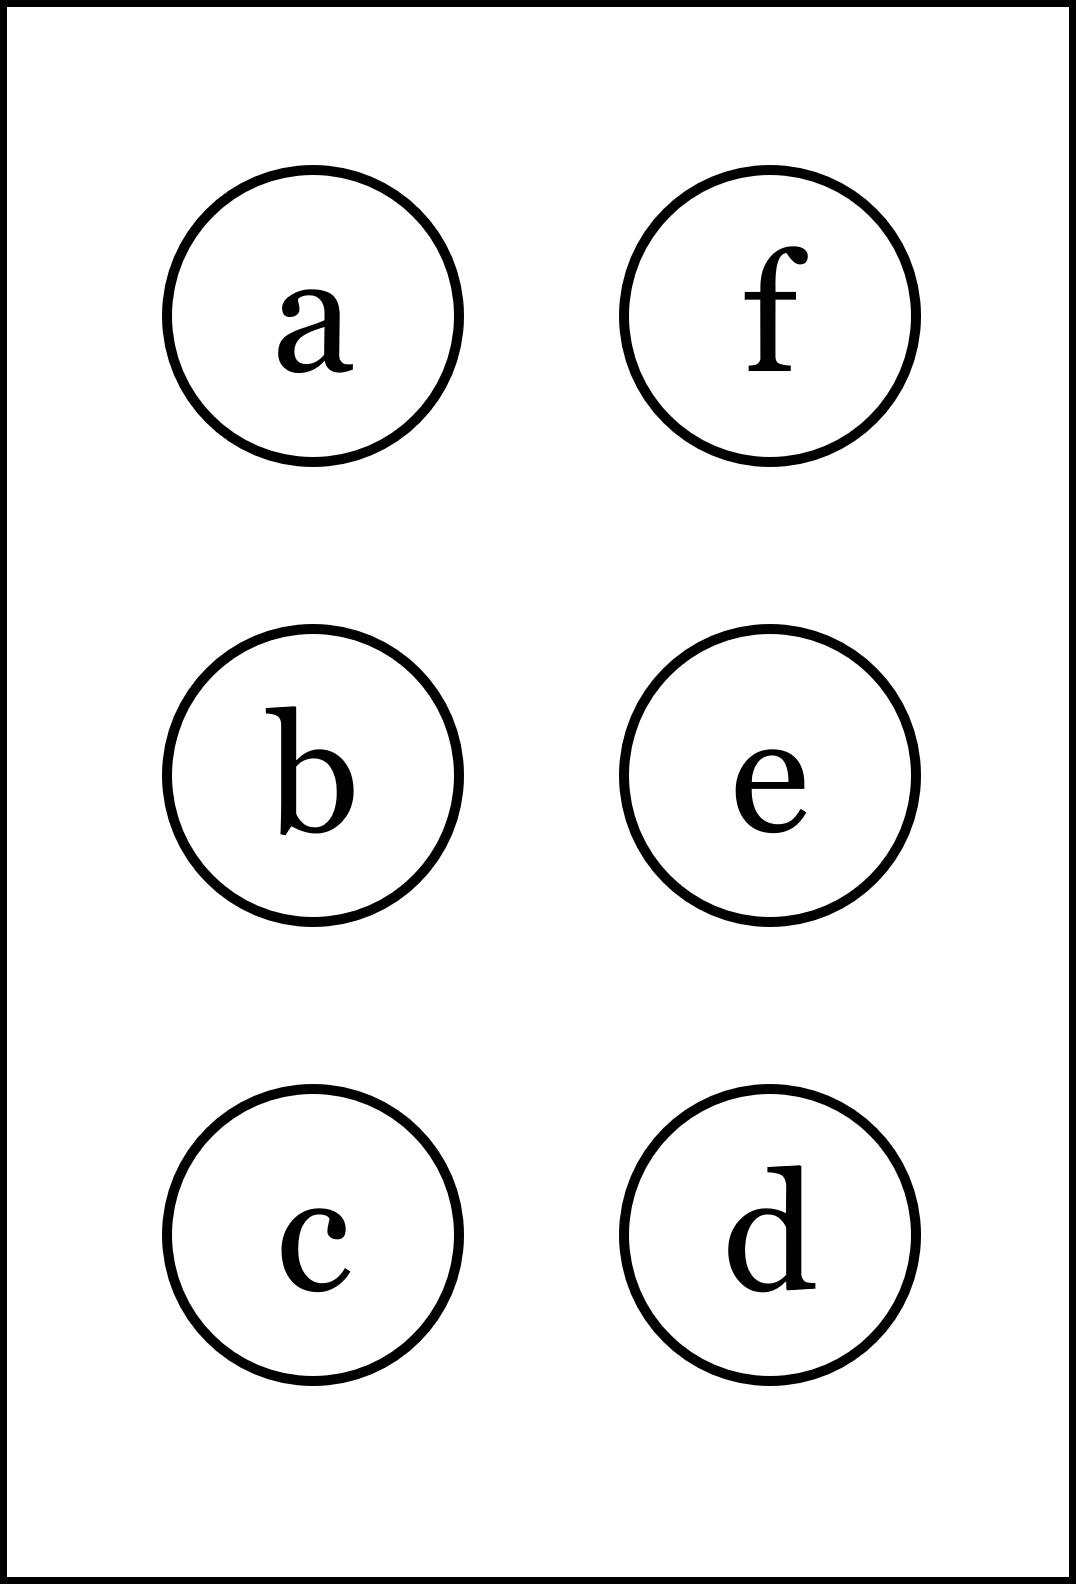
\includegraphics[height=40mm]{../images/braille.png}
{\small Písmeno Braillovej abecedy}
\end{center}
\end{minipage}
\end{center}
\end{minipage}
&
\begin{minipage}[c][104.5mm][t]{0.5\linewidth}
\begin{center}
\vspace{7mm}
{\huge Tečna funkce, skupina \textit{Delta $\delta$} -\romannumeral2}\\[5mm]
\textit{Meno:}\phantom{xxxxxxxxxxxxxxxxxxxxxxxxxxxxxxxxxxxxxxxxxxxxxxxxxxxxxxxxxxxxxxxxx}\\[5mm]
\begin{minipage}{0.95\linewidth}
\begin{center}
V \textbf{(a)} a \textbf{(b)} urči \text{rovnicu tečny} $y = kx + q$ ku funkci $f(x)$ v bode $x_0$.\\V \textbf{(c)} a \textbf{(d)} urči ypsilonové souřadnice bodů, ve kterých je sklon $f(x)$ rovný $k$.\\Pokud se výsledky shodujú s těmi za otazníky, tak napravo obarvi\\příslušející kroužek načerno. \textbf{Spolu odevzdejte výsledné slovo}.
\end{center}
\end{minipage}
\\[1mm]
\begin{minipage}{0.79\linewidth}
\begin{center}
\begin{varwidth}{\linewidth}
\begin{enumerate}
\small
\item $f(x)=\cfrac{-5x-1}{x+1}\enspace , \enspace x_0=3$\quad \dotfill\; ???\;\dotfill \quad $y = -\frac{1}{4}x-\frac{13}{4}$
\item $f(x)=-\sqrt{x-1}\enspace , \enspace x_0=82$\quad \dotfill\; ???\;\dotfill \quad $y = -\frac{1}{18}x-\frac{40}{9}$
\item $f(x)=4x^2-2x-2\enspace , \enspace k=5$\quad \dotfill\; ???\;\dotfill \quad $-\frac{11}{16}$
\item $f(x)=x^3-3x^2-23x-5\enspace , \enspace k=1$\quad \dotfill\; ???\;\dotfill \quad $21 , 103$
\item \quad \dotfill\; ???\;\dotfill \quad nebarvi
\item \quad \dotfill\; ???\;\dotfill \quad nebarvi
\end{enumerate}
\end{varwidth}
\end{center}
\end{minipage}
\begin{minipage}{0.20\linewidth}
\begin{center}
{\Huge\bfseries 2.} \\[2mm]
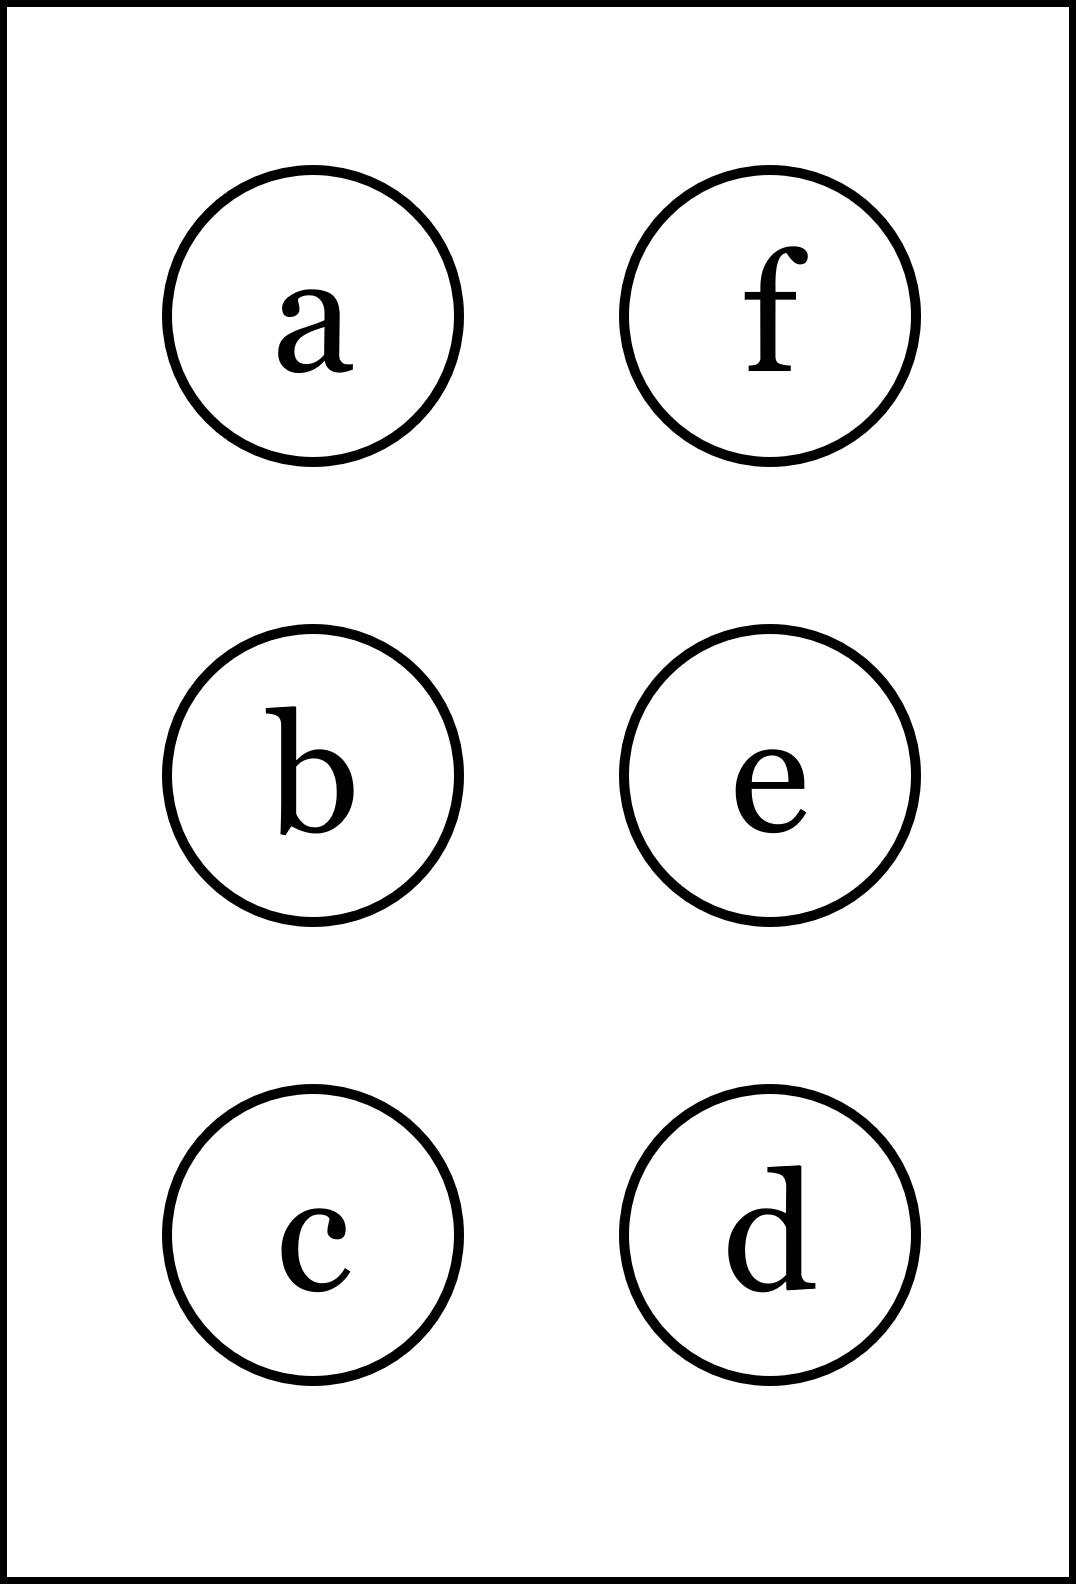
\includegraphics[height=40mm]{../images/braille.png}
{\small Písmeno Braillovej abecedy}
\end{center}
\end{minipage}
\end{center}
\end{minipage}
\\ \hdashline
\begin{minipage}[c][104.5mm][t]{0.5\linewidth}
\begin{center}
\vspace{7mm}
{\huge Tečna funkce, skupina \textit{Delta $\delta$} -\romannumeral3}\\[5mm]
\textit{Meno:}\phantom{xxxxxxxxxxxxxxxxxxxxxxxxxxxxxxxxxxxxxxxxxxxxxxxxxxxxxxxxxxxxxxxxx}\\[5mm]
\begin{minipage}{0.95\linewidth}
\begin{center}
V \textbf{(a)} a \textbf{(b)} urči \text{rovnicu tečny} $y = kx + q$ ku funkci $f(x)$ v bode $x_0$.\\V \textbf{(c)} a \textbf{(d)} urči ypsilonové souřadnice bodů, ve kterých je sklon $f(x)$ rovný $k$.\\Pokud se výsledky shodujú s těmi za otazníky, tak napravo obarvi\\příslušející kroužek načerno. \textbf{Spolu odevzdejte výsledné slovo}.
\end{center}
\end{minipage}
\\[1mm]
\begin{minipage}{0.79\linewidth}
\begin{center}
\begin{varwidth}{\linewidth}
\begin{enumerate}
\small
\item $f(x)=\cfrac{8x+8}{3x-3}\enspace , \enspace x_0=-1$\quad \dotfill\; ???\;\dotfill \quad $y = -\frac{4}{3}x-\frac{4}{3}$
\item $f(x)=5\sqrt{-5x+1}\enspace , \enspace x_0=0$\quad \dotfill\; ???\;\dotfill \quad $y = -\frac{25}{2}x+10$
\item $f(x)=-3x^2+x+6\enspace , \enspace k=-2$\quad \dotfill\; ???\;\dotfill \quad $-\frac{25}{4}$
\item $f(x)=3x^3-18x^2+30x+5\enspace , \enspace k=3$\quad \dotfill\; ???\;\dotfill \quad $20 , -166$
\item \quad \dotfill\; ???\;\dotfill \quad nebarvi
\item \quad \dotfill\; ???\;\dotfill \quad nebarvi
\end{enumerate}
\end{varwidth}
\end{center}
\end{minipage}
\begin{minipage}{0.20\linewidth}
\begin{center}
{\Huge\bfseries 3.} \\[2mm]
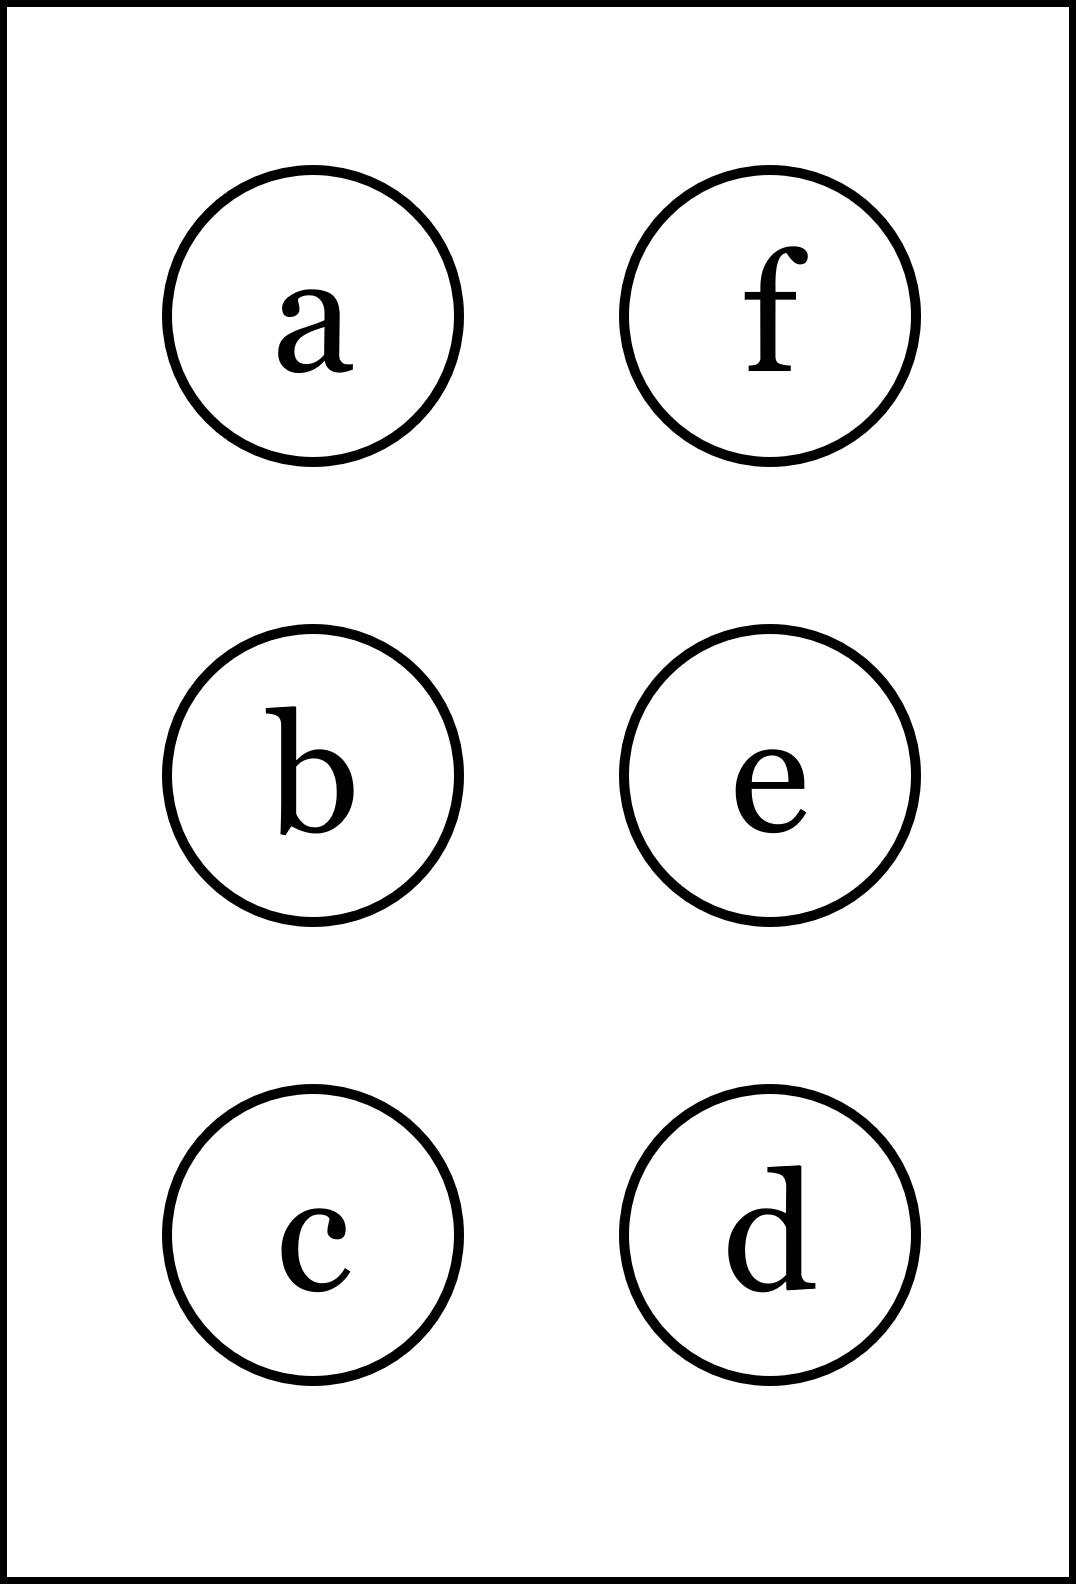
\includegraphics[height=40mm]{../images/braille.png}
{\small Písmeno Braillovej abecedy}
\end{center}
\end{minipage}
\end{center}
\end{minipage}
&
\begin{minipage}[c][104.5mm][t]{0.5\linewidth}
\begin{center}
\vspace{7mm}
{\huge Tečna funkce, skupina \textit{Delta $\delta$} -\romannumeral4}\\[5mm]
\textit{Meno:}\phantom{xxxxxxxxxxxxxxxxxxxxxxxxxxxxxxxxxxxxxxxxxxxxxxxxxxxxxxxxxxxxxxxxx}\\[5mm]
\begin{minipage}{0.95\linewidth}
\begin{center}
V \textbf{(a)} a \textbf{(b)} urči \text{rovnicu tečny} $y = kx + q$ ku funkci $f(x)$ v bode $x_0$.\\V \textbf{(c)} a \textbf{(d)} urči ypsilonové souřadnice bodů, ve kterých je sklon $f(x)$ rovný $k$.\\Pokud se výsledky shodujú s těmi za otazníky, tak napravo obarvi\\příslušející kroužek načerno. \textbf{Spolu odevzdejte výsledné slovo}.
\end{center}
\end{minipage}
\\[1mm]
\begin{minipage}{0.79\linewidth}
\begin{center}
\begin{varwidth}{\linewidth}
\begin{enumerate}
\small
\item $f(x)=\cfrac{2x-1}{-x+8}\enspace , \enspace x_0=7$\quad \dotfill\; ???\;\dotfill \quad $y = 15x-92$
\item $f(x)=-4\sqrt{-5x+6}\enspace , \enspace x_0=\frac{2}{5}$\quad \dotfill\; ???\;\dotfill \quad $y = 5x-20$
\item $f(x)=-6x^2+6x-4\enspace , \enspace k=-6$\quad \dotfill\; ???\;\dotfill \quad $-4$
\item $f(x)=x^3-3x^2-20x+1\enspace , \enspace k=4$\quad \dotfill\; ???\;\dotfill \quad $21 , 97$
\item \quad \dotfill\; ???\;\dotfill \quad nebarvi
\item \quad \dotfill\; ???\;\dotfill \quad nebarvi
\end{enumerate}
\end{varwidth}
\end{center}
\end{minipage}
\begin{minipage}{0.20\linewidth}
\begin{center}
{\Huge\bfseries 4.} \\[2mm]
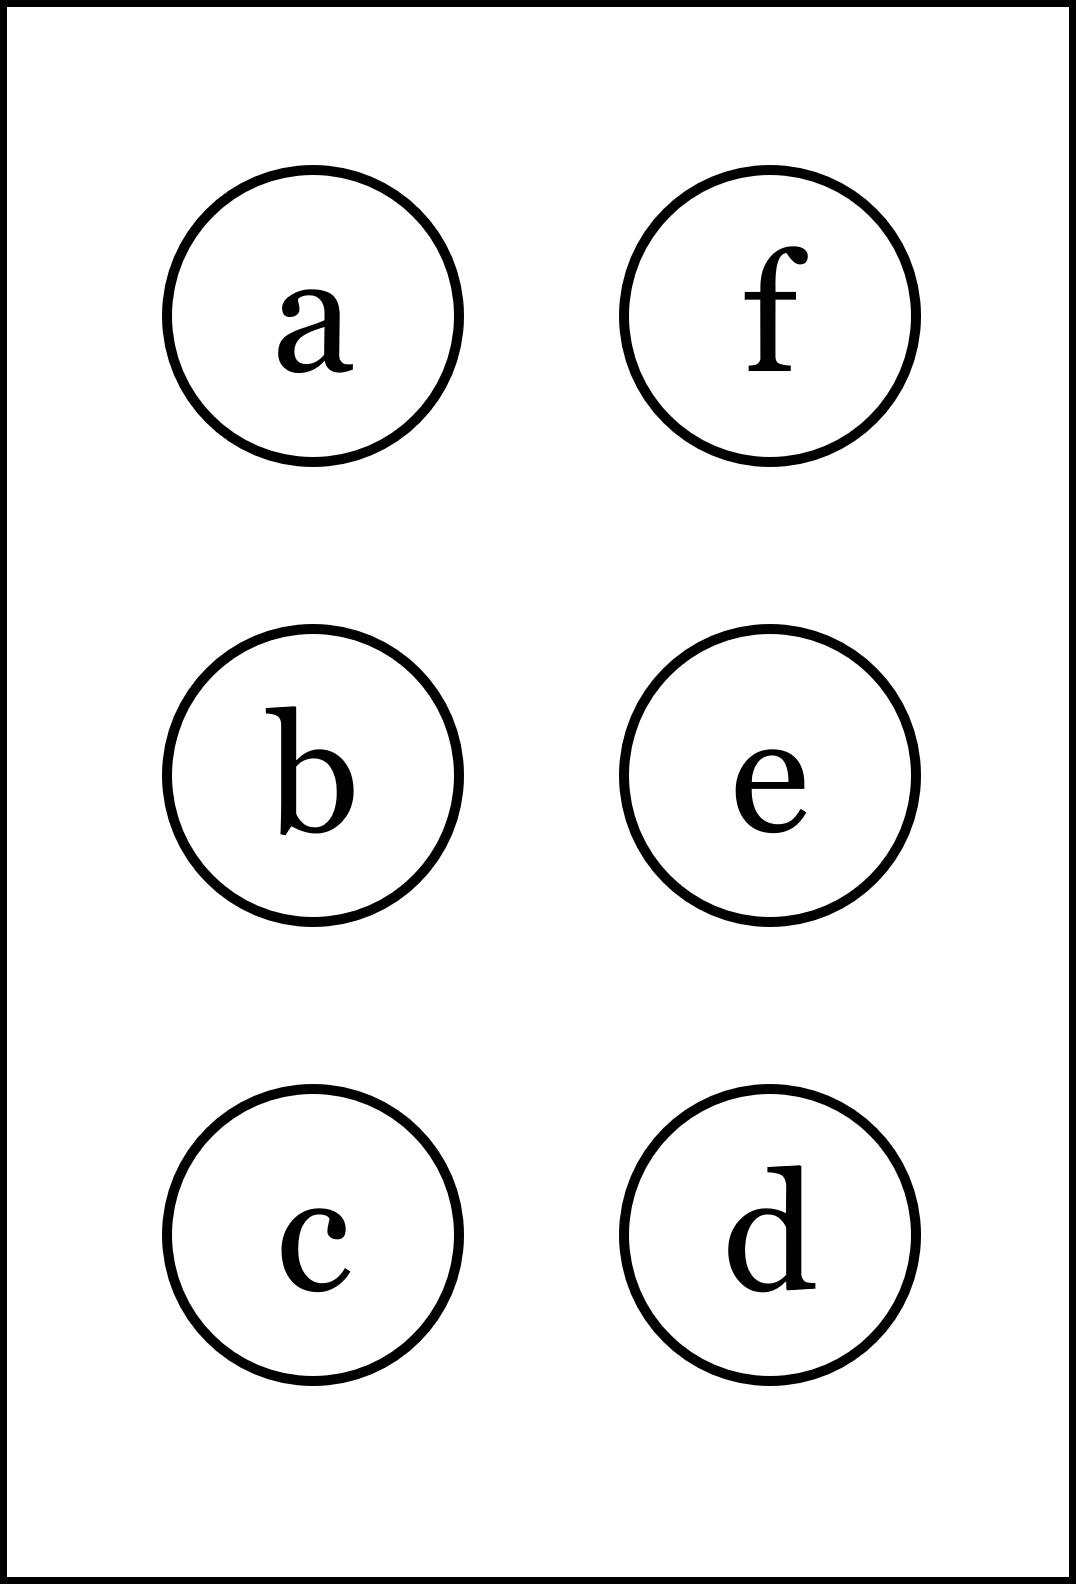
\includegraphics[height=40mm]{../images/braille.png}
{\small Písmeno Braillovej abecedy}
\end{center}
\end{minipage}
\end{center}
\end{minipage}
%
\end{tabular}
\newpage
\thispagestyle{empty}
\begin{tabular}{c:c}
\begin{minipage}[c][104.5mm][t]{0.5\linewidth}
\begin{center}
\vspace{7mm}
{\huge Tečna funkce, skupina \textit{Epsilon $\epsilon$} -\romannumeral1}\\[5mm]
\textit{Meno:}\phantom{xxxxxxxxxxxxxxxxxxxxxxxxxxxxxxxxxxxxxxxxxxxxxxxxxxxxxxxxxxxxxxxxx}\\[5mm]
\begin{minipage}{0.95\linewidth}
\begin{center}
V \textbf{(a)} a \textbf{(b)} urči \text{rovnicu tečny} $y = kx + q$ ku funkci $f(x)$ v bode $x_0$.\\V \textbf{(c)} a \textbf{(d)} urči ypsilonové souřadnice bodů, ve kterých je sklon $f(x)$ rovný $k$.\\Pokud se výsledky shodujú s těmi za otazníky, tak napravo obarvi\\příslušející kroužek načerno. \textbf{Spolu odevzdejte výsledné slovo}.
\end{center}
\end{minipage}
\\[1mm]
\begin{minipage}{0.79\linewidth}
\begin{center}
\begin{varwidth}{\linewidth}
\begin{enumerate}
\small
\item $f(x)=\cfrac{-2x+3}{-5x-1}\enspace , \enspace x_0=1$\quad \dotfill\; ???\;\dotfill \quad $y = \frac{17}{36}x-\frac{23}{36}$
\item $f(x)=\sqrt{4x-8}\enspace , \enspace x_0=\frac{33}{4}$\quad \dotfill\; ???\;\dotfill \quad $y = \frac{2}{5}x+\frac{17}{5}$
\item $f(x)=-5x^2-2x+7\enspace , \enspace k=-6$\quad \dotfill\; ???\;\dotfill \quad $-\frac{43}{5}$
\item $f(x)=4x^3-12x^2-95x-5\enspace , \enspace k=1$\quad \dotfill\; ???\;\dotfill \quad $105 , 439$
\item \quad \dotfill\; ???\;\dotfill \quad nebarvi
\item \quad \dotfill\; ???\;\dotfill \quad vybarvi
\end{enumerate}
\end{varwidth}
\end{center}
\end{minipage}
\begin{minipage}{0.20\linewidth}
\begin{center}
{\Huge\bfseries 1.} \\[2mm]
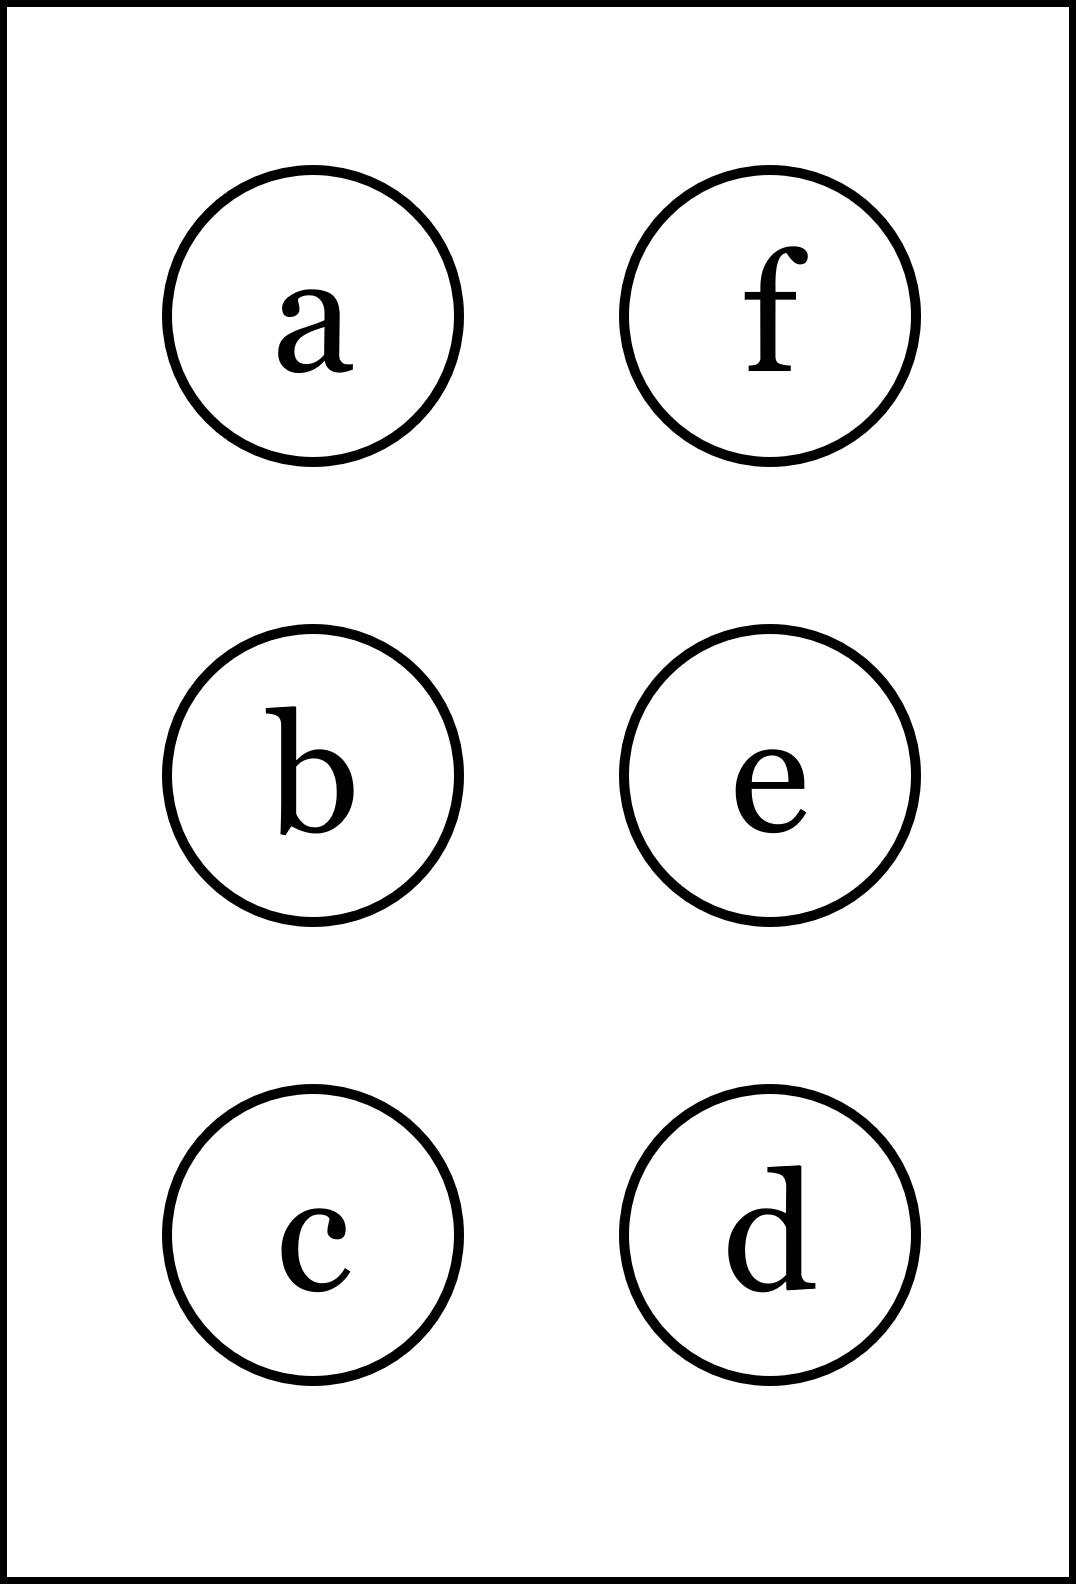
\includegraphics[height=40mm]{../images/braille.png}
{\small Písmeno Braillovej abecedy}
\end{center}
\end{minipage}
\end{center}
\end{minipage}
&
\begin{minipage}[c][104.5mm][t]{0.5\linewidth}
\begin{center}
\vspace{7mm}
{\huge Tečna funkce, skupina \textit{Epsilon $\epsilon$} -\romannumeral2}\\[5mm]
\textit{Meno:}\phantom{xxxxxxxxxxxxxxxxxxxxxxxxxxxxxxxxxxxxxxxxxxxxxxxxxxxxxxxxxxxxxxxxx}\\[5mm]
\begin{minipage}{0.95\linewidth}
\begin{center}
V \textbf{(a)} a \textbf{(b)} urči \text{rovnicu tečny} $y = kx + q$ ku funkci $f(x)$ v bode $x_0$.\\V \textbf{(c)} a \textbf{(d)} urči ypsilonové souřadnice bodů, ve kterých je sklon $f(x)$ rovný $k$.\\Pokud se výsledky shodujú s těmi za otazníky, tak napravo obarvi\\příslušející kroužek načerno. \textbf{Spolu odevzdejte výsledné slovo}.
\end{center}
\end{minipage}
\\[1mm]
\begin{minipage}{0.79\linewidth}
\begin{center}
\begin{varwidth}{\linewidth}
\begin{enumerate}
\small
\item $f(x)=\cfrac{-8x+1}{-3x+2}\enspace , \enspace x_0=2$\quad \dotfill\; ???\;\dotfill \quad $y = -\frac{13}{16}x+\frac{43}{8}$
\item $f(x)=\sqrt{-4x-1}\enspace , \enspace x_0=-\frac{1}{2}$\quad \dotfill\; ???\;\dotfill \quad $y = -2x+0$
\item $f(x)=3x^2+4x-2\enspace , \enspace k=-8$\quad \dotfill\; ???\;\dotfill \quad $2$
\item $f(x)=4x^3-24x^2-142x-2\enspace , \enspace k=2$\quad \dotfill\; ???\;\dotfill \quad $154 , -854$
\item \quad \dotfill\; ???\;\dotfill \quad nebarvi
\item \quad \dotfill\; ???\;\dotfill \quad nebarvi
\end{enumerate}
\end{varwidth}
\end{center}
\end{minipage}
\begin{minipage}{0.20\linewidth}
\begin{center}
{\Huge\bfseries 2.} \\[2mm]
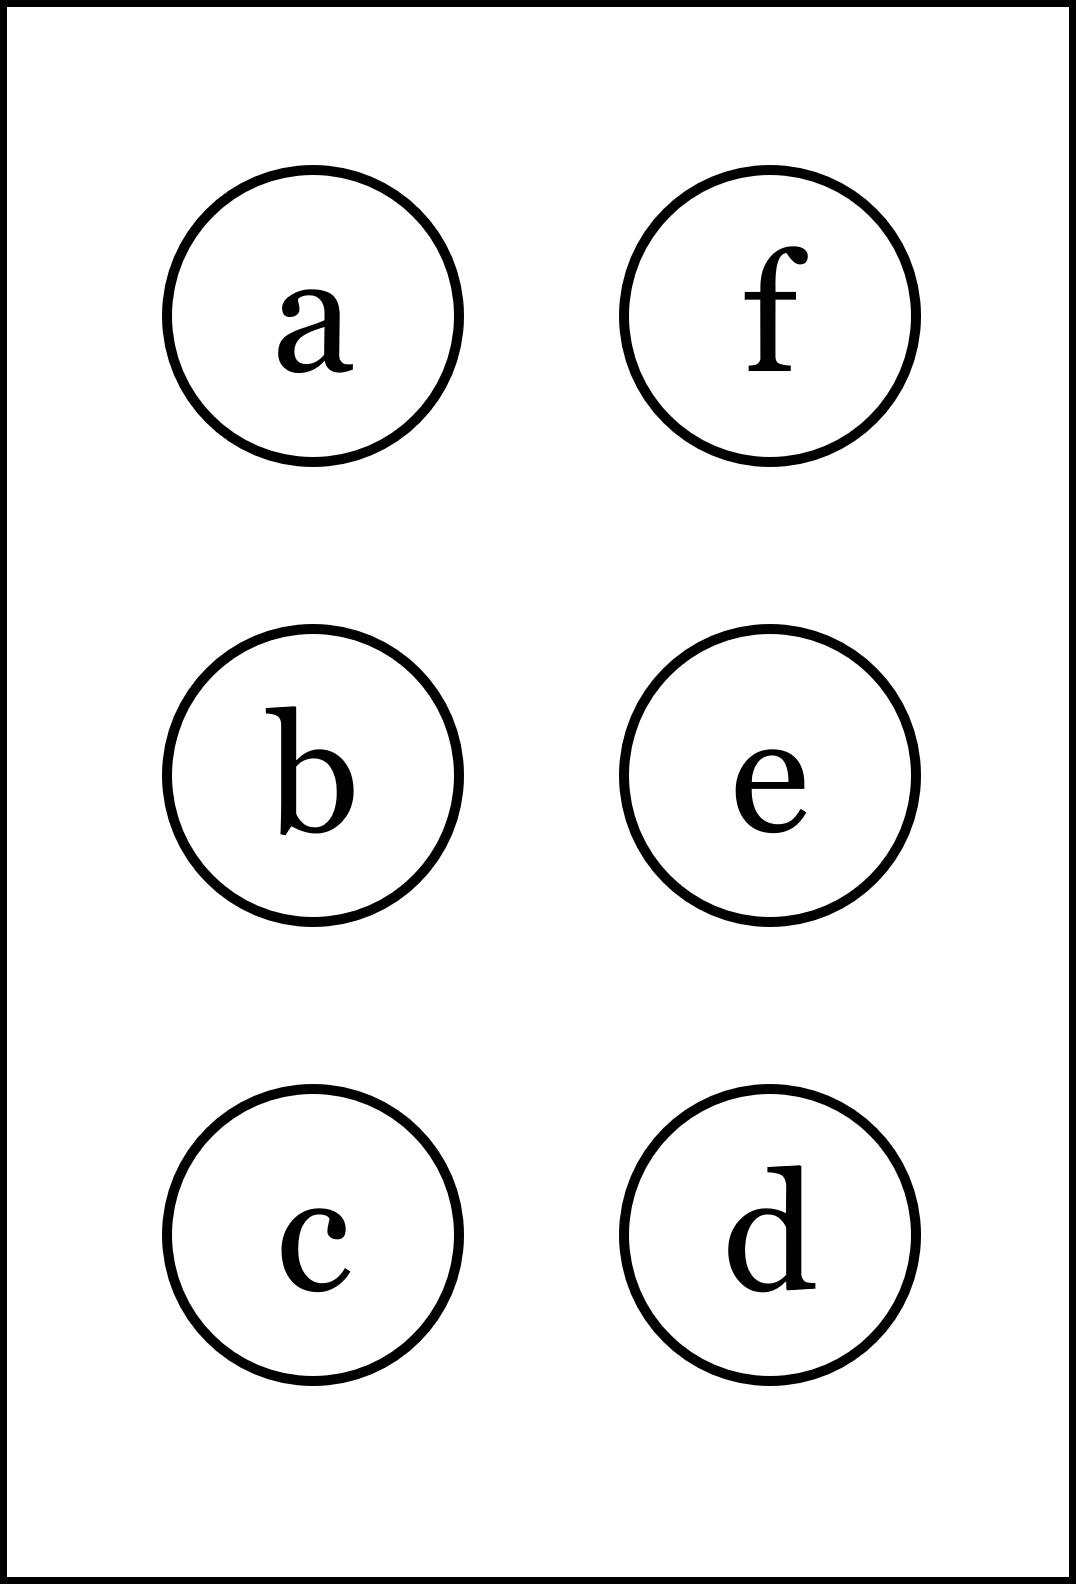
\includegraphics[height=40mm]{../images/braille.png}
{\small Písmeno Braillovej abecedy}
\end{center}
\end{minipage}
\end{center}
\end{minipage}
\\ \hdashline
\begin{minipage}[c][104.5mm][t]{0.5\linewidth}
\begin{center}
\vspace{7mm}
{\huge Tečna funkce, skupina \textit{Epsilon $\epsilon$} -\romannumeral3}\\[5mm]
\textit{Meno:}\phantom{xxxxxxxxxxxxxxxxxxxxxxxxxxxxxxxxxxxxxxxxxxxxxxxxxxxxxxxxxxxxxxxxx}\\[5mm]
\begin{minipage}{0.95\linewidth}
\begin{center}
V \textbf{(a)} a \textbf{(b)} urči \text{rovnicu tečny} $y = kx + q$ ku funkci $f(x)$ v bode $x_0$.\\V \textbf{(c)} a \textbf{(d)} urči ypsilonové souřadnice bodů, ve kterých je sklon $f(x)$ rovný $k$.\\Pokud se výsledky shodujú s těmi za otazníky, tak napravo obarvi\\příslušející kroužek načerno. \textbf{Spolu odevzdejte výsledné slovo}.
\end{center}
\end{minipage}
\\[1mm]
\begin{minipage}{0.79\linewidth}
\begin{center}
\begin{varwidth}{\linewidth}
\begin{enumerate}
\small
\item $f(x)=\cfrac{-2x+7}{-x+4}\enspace , \enspace x_0=-2$\quad \dotfill\; ???\;\dotfill \quad $y = -\frac{1}{36}x+\frac{16}{9}$
\item $f(x)=-3\sqrt{-2x-2}\enspace , \enspace x_0=-\frac{27}{2}$\quad \dotfill\; ???\;\dotfill \quad $y = \frac{3}{5}x-\frac{69}{5}$
\item $f(x)=4x^2-4x-6\enspace , \enspace k=5$\quad \dotfill\; ???\;\dotfill \quad $-\frac{87}{16}$
\item $f(x)=2x^3-12x^2-32x-1\enspace , \enspace k=-2$\quad \dotfill\; ???\;\dotfill \quad $17 , 109$
\item \quad \dotfill\; ???\;\dotfill \quad nebarvi
\item \quad \dotfill\; ???\;\dotfill \quad nebarvi
\end{enumerate}
\end{varwidth}
\end{center}
\end{minipage}
\begin{minipage}{0.20\linewidth}
\begin{center}
{\Huge\bfseries 3.} \\[2mm]
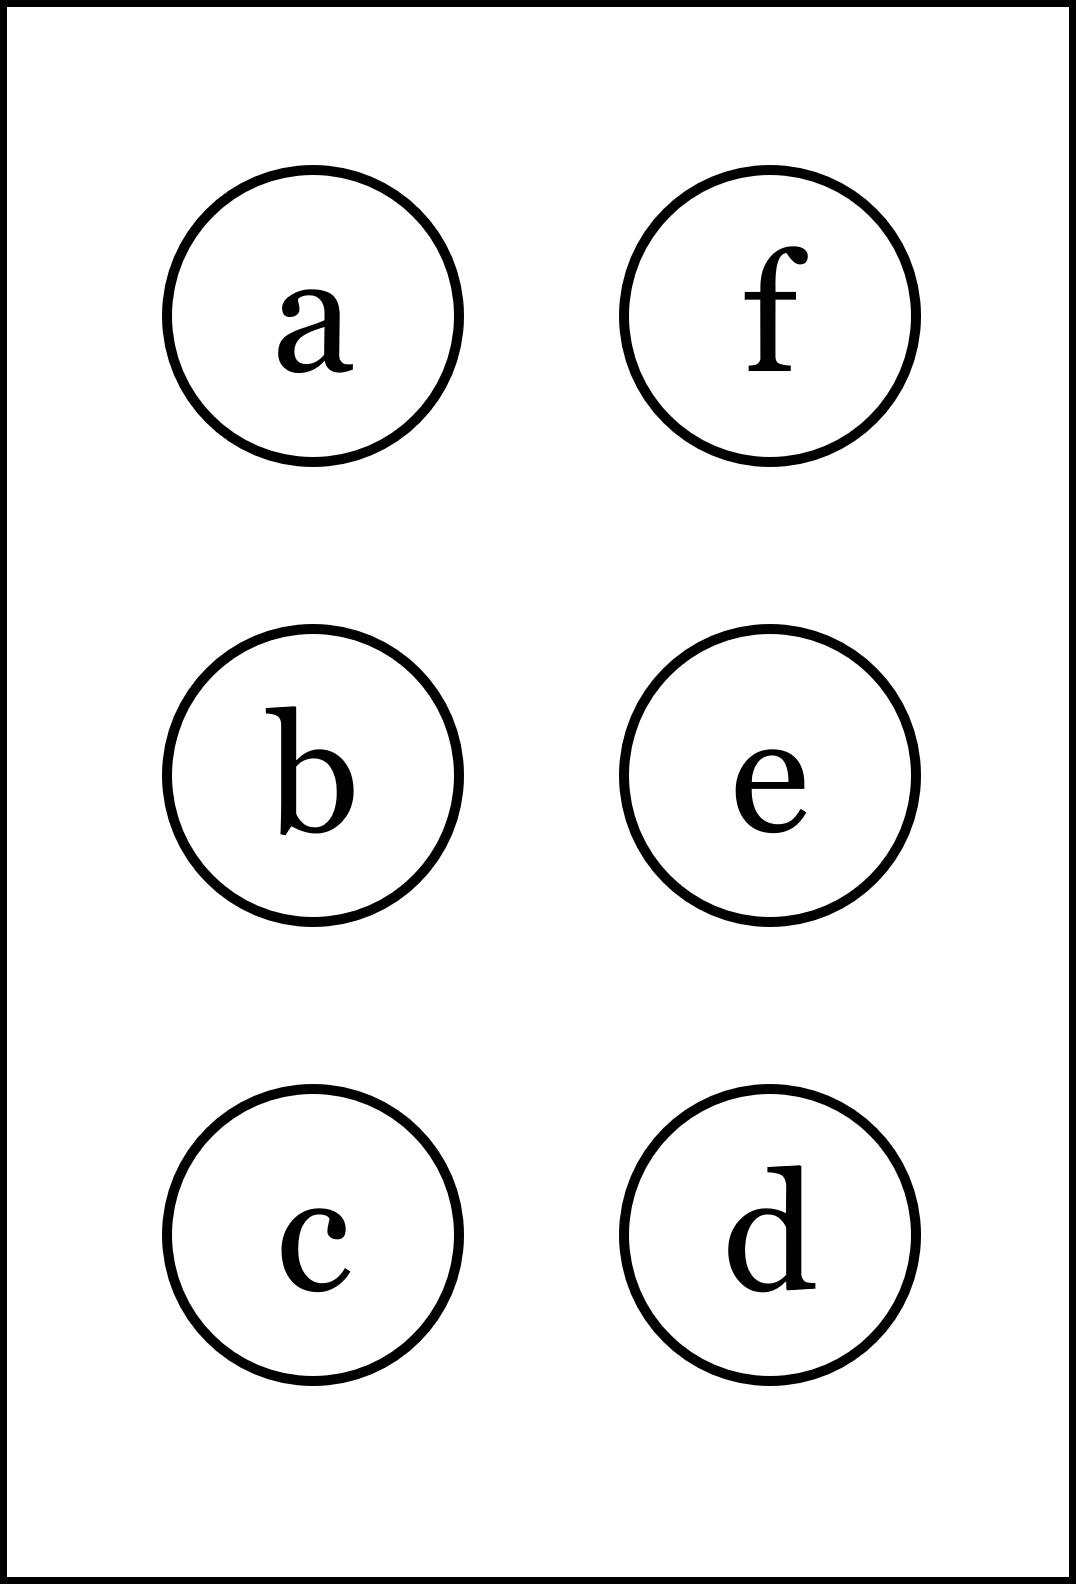
\includegraphics[height=40mm]{../images/braille.png}
{\small Písmeno Braillovej abecedy}
\end{center}
\end{minipage}
\end{center}
\end{minipage}
&
\begin{minipage}[c][104.5mm][t]{0.5\linewidth}
\begin{center}
\vspace{7mm}
{\huge Tečna funkce, skupina \textit{Epsilon $\epsilon$} -\romannumeral4}\\[5mm]
\textit{Meno:}\phantom{xxxxxxxxxxxxxxxxxxxxxxxxxxxxxxxxxxxxxxxxxxxxxxxxxxxxxxxxxxxxxxxxx}\\[5mm]
\begin{minipage}{0.95\linewidth}
\begin{center}
V \textbf{(a)} a \textbf{(b)} urči \text{rovnicu tečny} $y = kx + q$ ku funkci $f(x)$ v bode $x_0$.\\V \textbf{(c)} a \textbf{(d)} urči ypsilonové souřadnice bodů, ve kterých je sklon $f(x)$ rovný $k$.\\Pokud se výsledky shodujú s těmi za otazníky, tak napravo obarvi\\příslušející kroužek načerno. \textbf{Spolu odevzdejte výsledné slovo}.
\end{center}
\end{minipage}
\\[1mm]
\begin{minipage}{0.79\linewidth}
\begin{center}
\begin{varwidth}{\linewidth}
\begin{enumerate}
\small
\item $f(x)=\cfrac{-3x-4}{x+5}\enspace , \enspace x_0=-2$\quad \dotfill\; ???\;\dotfill \quad $y = -\frac{11}{9}x-\frac{16}{9}$
\item $f(x)=3\sqrt{x-3}\enspace , \enspace x_0=28$\quad \dotfill\; ???\;\dotfill \quad $y = \frac{3}{10}x+\frac{33}{5}$
\item $f(x)=-2x^2+4x-1\enspace , \enspace k=-3$\quad \dotfill\; ???\;\dotfill \quad $-\frac{1}{8}$
\item $f(x)=x^3-3x^2-12x-2\enspace , \enspace k=-3$\quad \dotfill\; ???\;\dotfill \quad $6 , 34$
\item \quad \dotfill\; ???\;\dotfill \quad vybarvi
\item \quad \dotfill\; ???\;\dotfill \quad nebarvi
\end{enumerate}
\end{varwidth}
\end{center}
\end{minipage}
\begin{minipage}{0.20\linewidth}
\begin{center}
{\Huge\bfseries 4.} \\[2mm]
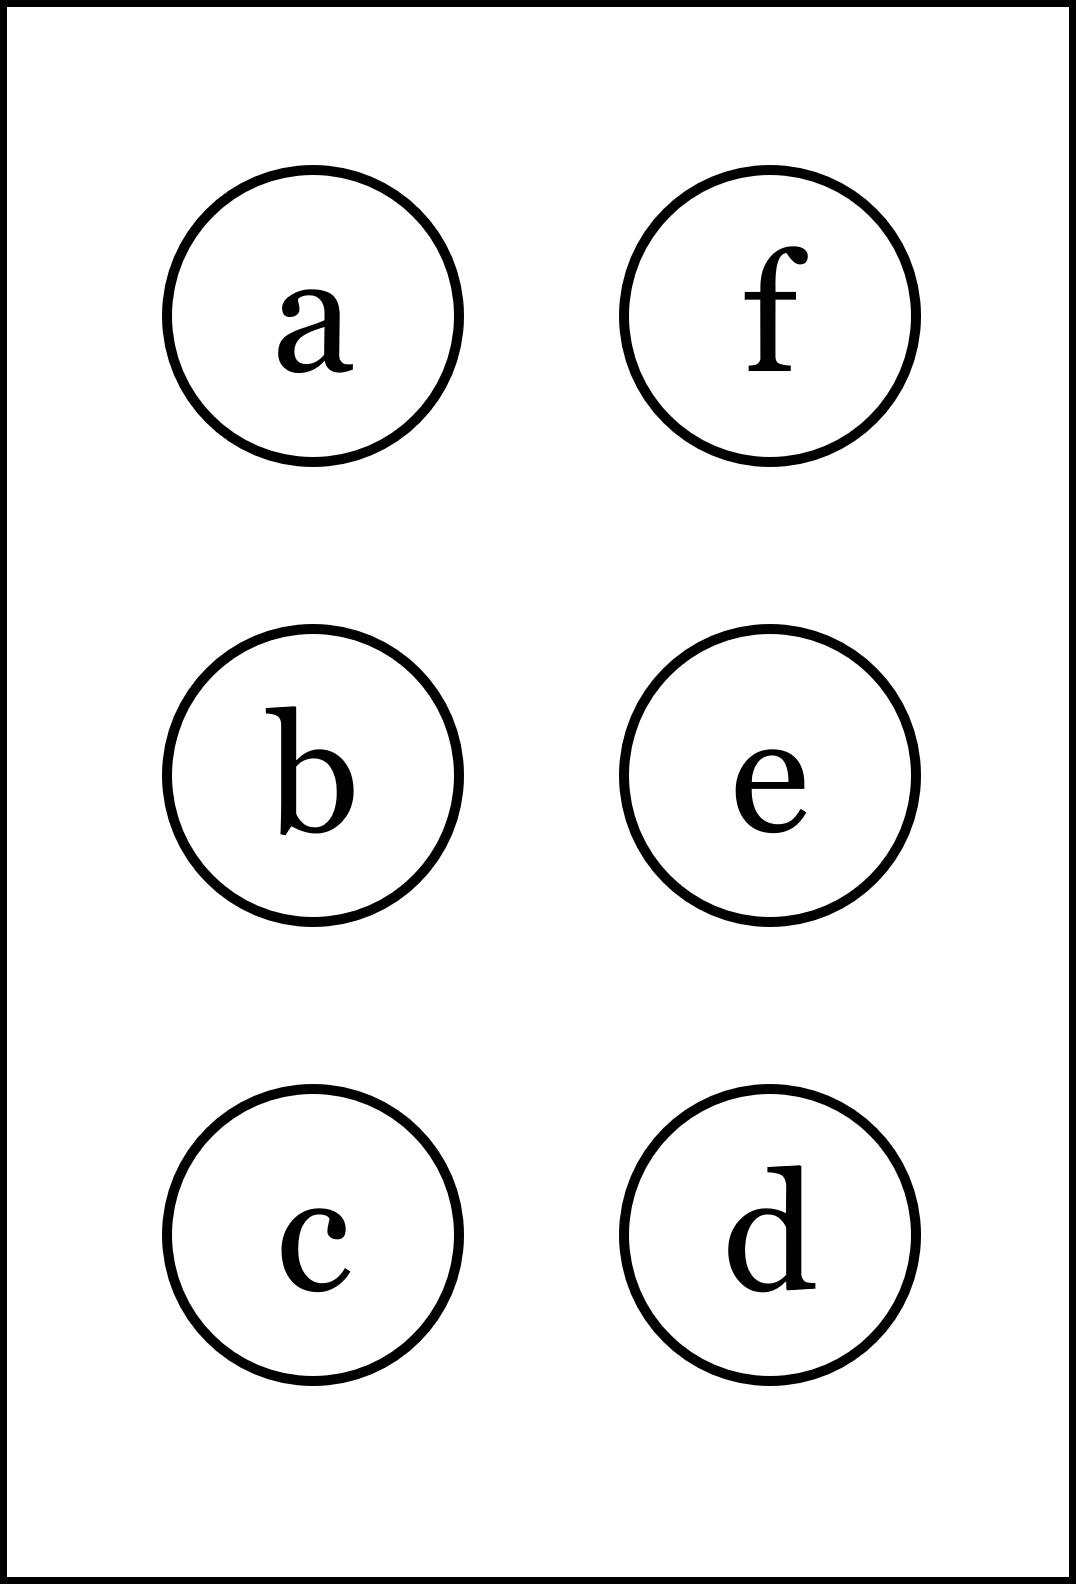
\includegraphics[height=40mm]{../images/braille.png}
{\small Písmeno Braillovej abecedy}
\end{center}
\end{minipage}
\end{center}
\end{minipage}
%
\end{tabular}
\newpage
\thispagestyle{empty}
\begin{tabular}{c:c}
\begin{minipage}[c][104.5mm][t]{0.5\linewidth}
\begin{center}
\vspace{7mm}
{\huge Tečna funkce, skupina \textit{Zeta $\zeta$} -\romannumeral1}\\[5mm]
\textit{Meno:}\phantom{xxxxxxxxxxxxxxxxxxxxxxxxxxxxxxxxxxxxxxxxxxxxxxxxxxxxxxxxxxxxxxxxx}\\[5mm]
\begin{minipage}{0.95\linewidth}
\begin{center}
V \textbf{(a)} a \textbf{(b)} urči \text{rovnicu tečny} $y = kx + q$ ku funkci $f(x)$ v bode $x_0$.\\V \textbf{(c)} a \textbf{(d)} urči ypsilonové souřadnice bodů, ve kterých je sklon $f(x)$ rovný $k$.\\Pokud se výsledky shodujú s těmi za otazníky, tak napravo obarvi\\příslušející kroužek načerno. \textbf{Spolu odevzdejte výsledné slovo}.
\end{center}
\end{minipage}
\\[1mm]
\begin{minipage}{0.79\linewidth}
\begin{center}
\begin{varwidth}{\linewidth}
\begin{enumerate}
\small
\item $f(x)=\cfrac{-4x-7}{x+6}\enspace , \enspace x_0=-1$\quad \dotfill\; ???\;\dotfill \quad $y = -\frac{17}{25}x-\frac{12}{5}$
\item $f(x)=-2\sqrt{5x-1}\enspace , \enspace x_0=10$\quad \dotfill\; ???\;\dotfill \quad $y = -\frac{5}{7}x-\frac{48}{7}$
\item $f(x)=5x^2+5x-2\enspace , \enspace k=1$\quad \dotfill\; ???\;\dotfill \quad $-\frac{16}{5}$
\item $f(x)=x^3-6x^2-12x-1\enspace , \enspace k=3$\quad \dotfill\; ???\;\dotfill \quad $4 , -86$
\item \quad \dotfill\; ???\;\dotfill \quad nebarvi
\item \quad \dotfill\; ???\;\dotfill \quad vybarvi
\end{enumerate}
\end{varwidth}
\end{center}
\end{minipage}
\begin{minipage}{0.20\linewidth}
\begin{center}
{\Huge\bfseries 1.} \\[2mm]
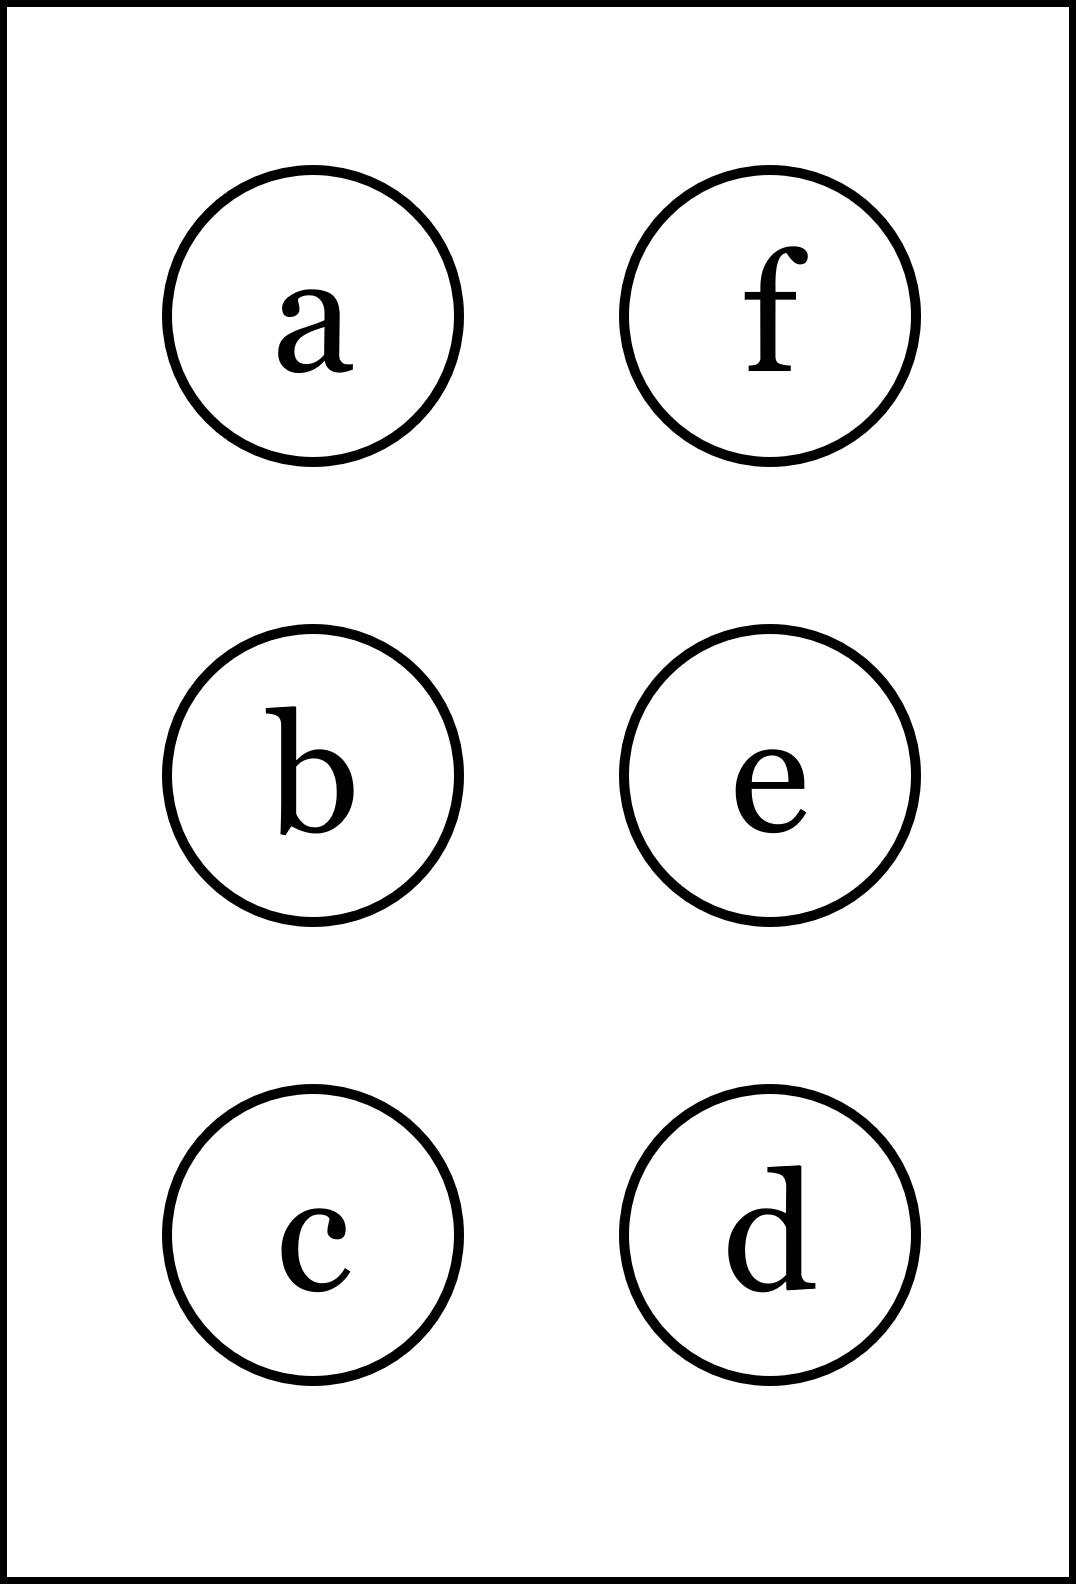
\includegraphics[height=40mm]{../images/braille.png}
{\small Písmeno Braillovej abecedy}
\end{center}
\end{minipage}
\end{center}
\end{minipage}
&
\begin{minipage}[c][104.5mm][t]{0.5\linewidth}
\begin{center}
\vspace{7mm}
{\huge Tečna funkce, skupina \textit{Zeta $\zeta$} -\romannumeral2}\\[5mm]
\textit{Meno:}\phantom{xxxxxxxxxxxxxxxxxxxxxxxxxxxxxxxxxxxxxxxxxxxxxxxxxxxxxxxxxxxxxxxxx}\\[5mm]
\begin{minipage}{0.95\linewidth}
\begin{center}
V \textbf{(a)} a \textbf{(b)} urči \text{rovnicu tečny} $y = kx + q$ ku funkci $f(x)$ v bode $x_0$.\\V \textbf{(c)} a \textbf{(d)} urči ypsilonové souřadnice bodů, ve kterých je sklon $f(x)$ rovný $k$.\\Pokud se výsledky shodujú s těmi za otazníky, tak napravo obarvi\\příslušející kroužek načerno. \textbf{Spolu odevzdejte výsledné slovo}.
\end{center}
\end{minipage}
\\[1mm]
\begin{minipage}{0.79\linewidth}
\begin{center}
\begin{varwidth}{\linewidth}
\begin{enumerate}
\small
\item $f(x)=\cfrac{6x+2}{4x+4}\enspace , \enspace x_0=1$\quad \dotfill\; ???\;\dotfill \quad $y = \frac{1}{4}x+\frac{3}{4}$
\item $f(x)=-3\sqrt{-4x+4}\enspace , \enspace x_0=-15$\quad \dotfill\; ???\;\dotfill \quad $y = \frac{3}{4}x-\frac{51}{4}$
\item $f(x)=8x^2+8x+2\enspace , \enspace k=-8$\quad \dotfill\; ???\;\dotfill \quad $2$
\item $f(x)=x^3-6x^2+10x+1\enspace , \enspace k=1$\quad \dotfill\; ???\;\dotfill \quad $6 , -56$
\item \quad \dotfill\; ???\;\dotfill \quad vybarvi
\item \quad \dotfill\; ???\;\dotfill \quad nebarvi
\end{enumerate}
\end{varwidth}
\end{center}
\end{minipage}
\begin{minipage}{0.20\linewidth}
\begin{center}
{\Huge\bfseries 2.} \\[2mm]
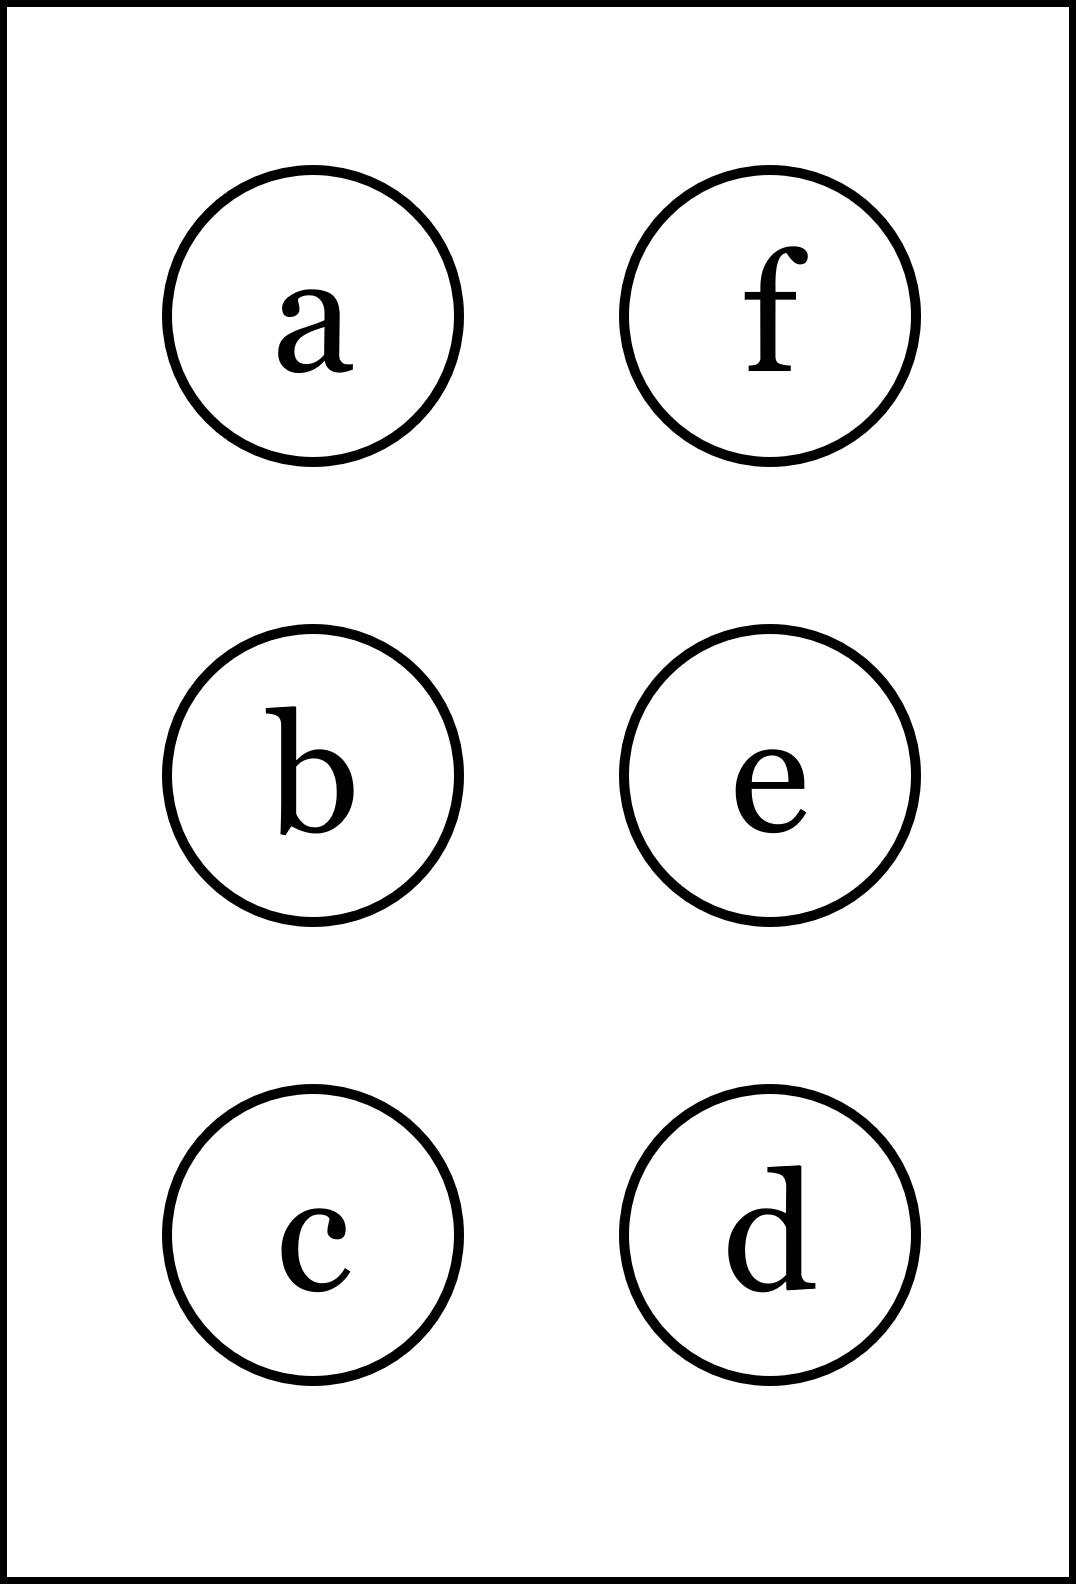
\includegraphics[height=40mm]{../images/braille.png}
{\small Písmeno Braillovej abecedy}
\end{center}
\end{minipage}
\end{center}
\end{minipage}
\\ \hdashline
\begin{minipage}[c][104.5mm][t]{0.5\linewidth}
\begin{center}
\vspace{7mm}
{\huge Tečna funkce, skupina \textit{Zeta $\zeta$} -\romannumeral3}\\[5mm]
\textit{Meno:}\phantom{xxxxxxxxxxxxxxxxxxxxxxxxxxxxxxxxxxxxxxxxxxxxxxxxxxxxxxxxxxxxxxxxx}\\[5mm]
\begin{minipage}{0.95\linewidth}
\begin{center}
V \textbf{(a)} a \textbf{(b)} urči \text{rovnicu tečny} $y = kx + q$ ku funkci $f(x)$ v bode $x_0$.\\V \textbf{(c)} a \textbf{(d)} urči ypsilonové souřadnice bodů, ve kterých je sklon $f(x)$ rovný $k$.\\Pokud se výsledky shodujú s těmi za otazníky, tak napravo obarvi\\příslušející kroužek načerno. \textbf{Spolu odevzdejte výsledné slovo}.
\end{center}
\end{minipage}
\\[1mm]
\begin{minipage}{0.79\linewidth}
\begin{center}
\begin{varwidth}{\linewidth}
\begin{enumerate}
\small
\item $f(x)=\cfrac{4x+2}{-3x+1}\enspace , \enspace x_0=1$\quad \dotfill\; ???\;\dotfill \quad $y = \frac{5}{2}x-\frac{11}{2}$
\item $f(x)=-6\sqrt{7x+1}\enspace , \enspace x_0=\frac{3}{7}$\quad \dotfill\; ???\;\dotfill \quad $y = -\frac{21}{2}x-15$
\item $f(x)=-x^2+7x+3\enspace , \enspace k=2$\quad \dotfill\; ???\;\dotfill \quad $\frac{33}{4}$
\item $f(x)=x^3-9x^2-52x+5\enspace , \enspace k=-4$\quad \dotfill\; ???\;\dotfill \quad $65 , -475$
\item \quad \dotfill\; ???\;\dotfill \quad nebarvi
\item \quad \dotfill\; ???\;\dotfill \quad nebarvi
\end{enumerate}
\end{varwidth}
\end{center}
\end{minipage}
\begin{minipage}{0.20\linewidth}
\begin{center}
{\Huge\bfseries 3.} \\[2mm]
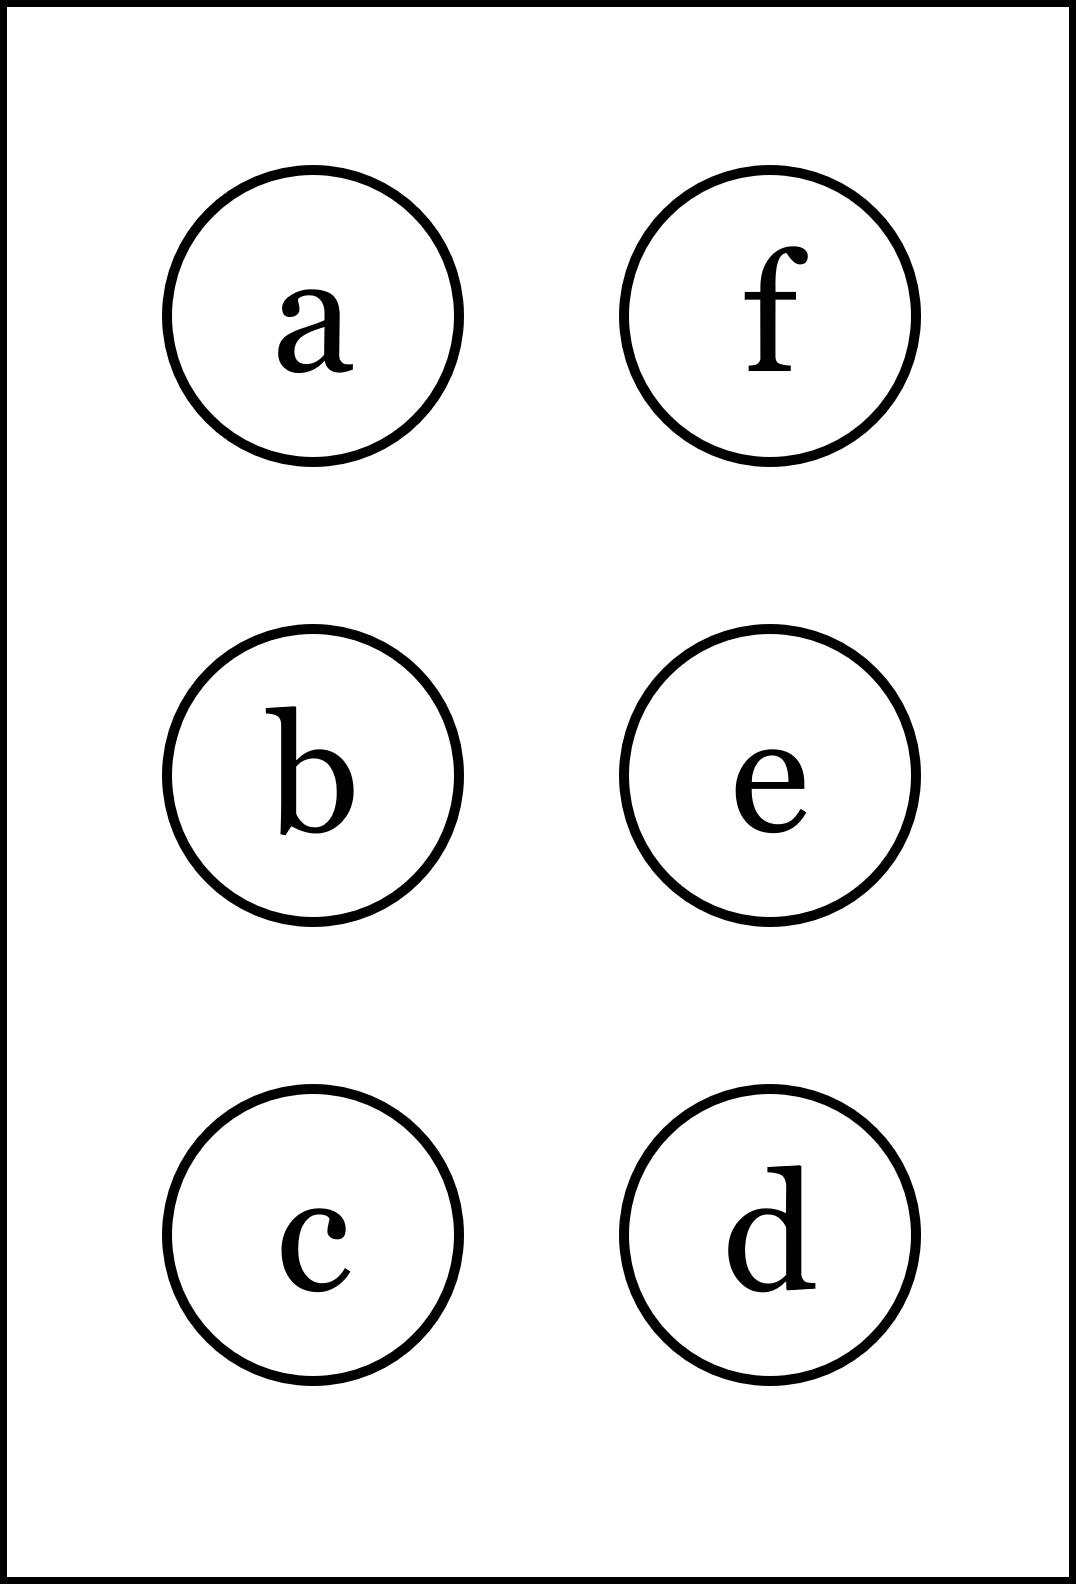
\includegraphics[height=40mm]{../images/braille.png}
{\small Písmeno Braillovej abecedy}
\end{center}
\end{minipage}
\end{center}
\end{minipage}
&
\begin{minipage}[c][104.5mm][t]{0.5\linewidth}
\begin{center}
\vspace{7mm}
{\huge Tečna funkce, skupina \textit{Zeta $\zeta$} -\romannumeral4}\\[5mm]
\textit{Meno:}\phantom{xxxxxxxxxxxxxxxxxxxxxxxxxxxxxxxxxxxxxxxxxxxxxxxxxxxxxxxxxxxxxxxxx}\\[5mm]
\begin{minipage}{0.95\linewidth}
\begin{center}
V \textbf{(a)} a \textbf{(b)} urči \text{rovnicu tečny} $y = kx + q$ ku funkci $f(x)$ v bode $x_0$.\\V \textbf{(c)} a \textbf{(d)} urči ypsilonové souřadnice bodů, ve kterých je sklon $f(x)$ rovný $k$.\\Pokud se výsledky shodujú s těmi za otazníky, tak napravo obarvi\\příslušející kroužek načerno. \textbf{Spolu odevzdejte výsledné slovo}.
\end{center}
\end{minipage}
\\[1mm]
\begin{minipage}{0.79\linewidth}
\begin{center}
\begin{varwidth}{\linewidth}
\begin{enumerate}
\small
\item $f(x)=\cfrac{2x-5}{2x+4}\enspace , \enspace x_0=3$\quad \dotfill\; ???\;\dotfill \quad $y = \frac{9}{50}x+\frac{19}{25}$
\item $f(x)=-4\sqrt{-2x+3}\enspace , \enspace x_0=-\frac{61}{2}$\quad \dotfill\; ???\;\dotfill \quad $y = \frac{1}{2}x-\frac{67}{4}$
\item $f(x)=4x^2+9x-9\enspace , \enspace k=1$\quad \dotfill\; ???\;\dotfill \quad $-14$
\item $f(x)=x^3-6x^2-16x-5\enspace , \enspace k=-1$\quad \dotfill\; ???\;\dotfill \quad $4 , 50$
\item \quad \dotfill\; ???\;\dotfill \quad vybarvi
\item \quad \dotfill\; ???\;\dotfill \quad vybarvi
\end{enumerate}
\end{varwidth}
\end{center}
\end{minipage}
\begin{minipage}{0.20\linewidth}
\begin{center}
{\Huge\bfseries 4.} \\[2mm]
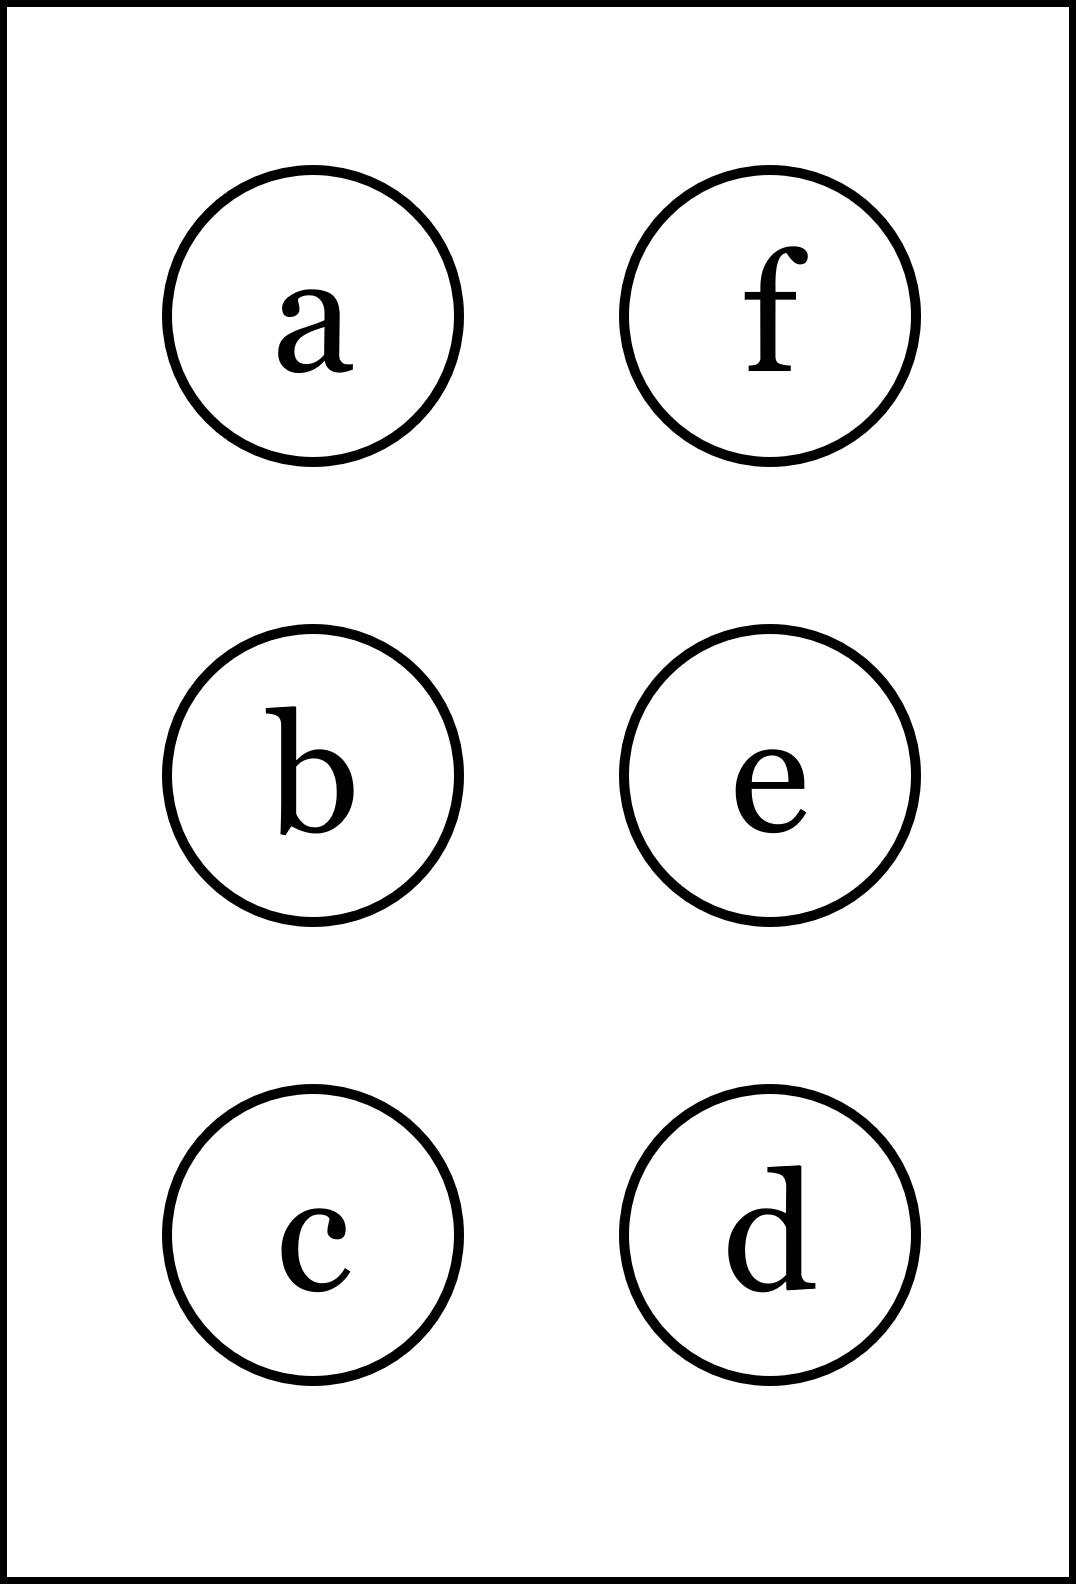
\includegraphics[height=40mm]{../images/braille.png}
{\small Písmeno Braillovej abecedy}
\end{center}
\end{minipage}
\end{center}
\end{minipage}
%
\end{tabular}
\newpage
\thispagestyle{empty}
\begin{tabular}{c:c}
\begin{minipage}[c][104.5mm][t]{0.5\linewidth}
\begin{center}
\vspace{7mm}
{\huge Tečna funkce, skupina \textit{Eta $\eta$} -\romannumeral1}\\[5mm]
\textit{Meno:}\phantom{xxxxxxxxxxxxxxxxxxxxxxxxxxxxxxxxxxxxxxxxxxxxxxxxxxxxxxxxxxxxxxxxx}\\[5mm]
\begin{minipage}{0.95\linewidth}
\begin{center}
V \textbf{(a)} a \textbf{(b)} urči \text{rovnicu tečny} $y = kx + q$ ku funkci $f(x)$ v bode $x_0$.\\V \textbf{(c)} a \textbf{(d)} urči ypsilonové souřadnice bodů, ve kterých je sklon $f(x)$ rovný $k$.\\Pokud se výsledky shodujú s těmi za otazníky, tak napravo obarvi\\příslušející kroužek načerno. \textbf{Spolu odevzdejte výsledné slovo}.
\end{center}
\end{minipage}
\\[1mm]
\begin{minipage}{0.79\linewidth}
\begin{center}
\begin{varwidth}{\linewidth}
\begin{enumerate}
\small
\item $f(x)=\cfrac{x+4}{7x-4}\enspace , \enspace x_0=-1$\quad \dotfill\; ???\;\dotfill \quad $y = -\frac{32}{121}x-\frac{65}{121}$
\item $f(x)=4\sqrt{-3x+3}\enspace , \enspace x_0=-\frac{61}{3}$\quad \dotfill\; ???\;\dotfill \quad $y = -\frac{3}{4}x+\frac{67}{2}$
\item $f(x)=-5x^2+7x+3\enspace , \enspace k=-4$\quad \dotfill\; ???\;\dotfill \quad $\frac{93}{20}$
\item $f(x)=2x^3-6x^2-13x-2\enspace , \enspace k=5$\quad \dotfill\; ???\;\dotfill \quad $3 , 37$
\item \quad \dotfill\; ???\;\dotfill \quad nebarvi
\item \quad \dotfill\; ???\;\dotfill \quad nebarvi
\end{enumerate}
\end{varwidth}
\end{center}
\end{minipage}
\begin{minipage}{0.20\linewidth}
\begin{center}
{\Huge\bfseries 1.} \\[2mm]
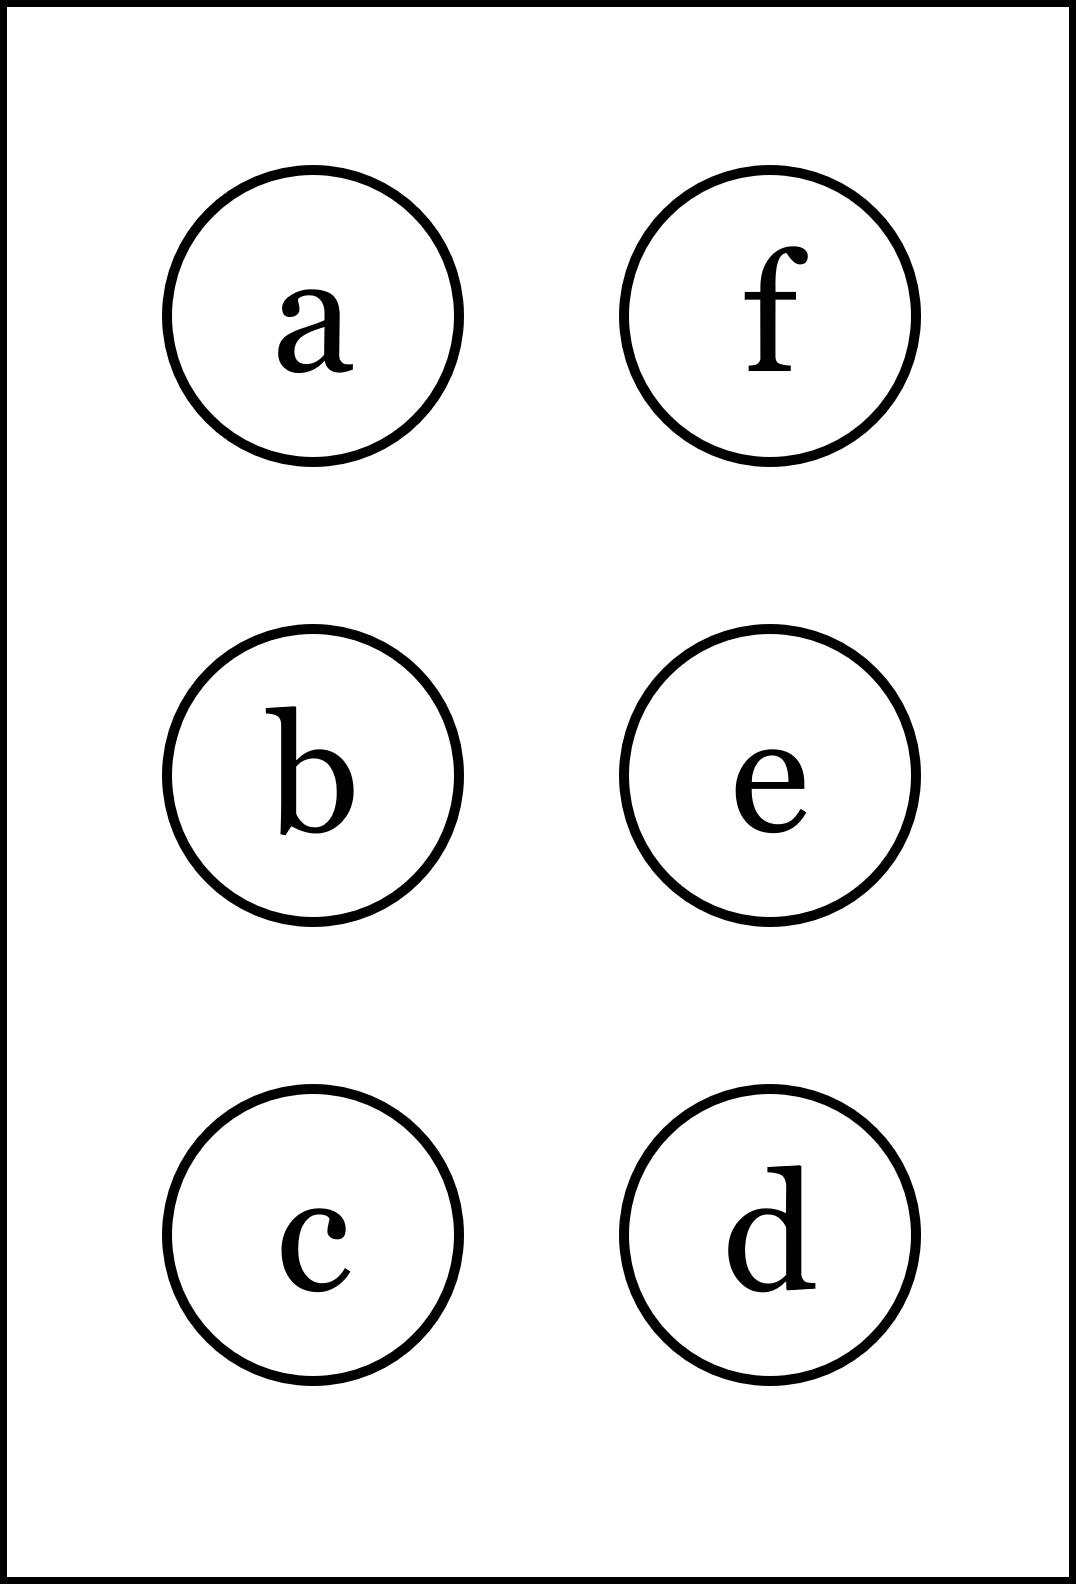
\includegraphics[height=40mm]{../images/braille.png}
{\small Písmeno Braillovej abecedy}
\end{center}
\end{minipage}
\end{center}
\end{minipage}
&
\begin{minipage}[c][104.5mm][t]{0.5\linewidth}
\begin{center}
\vspace{7mm}
{\huge Tečna funkce, skupina \textit{Eta $\eta$} -\romannumeral2}\\[5mm]
\textit{Meno:}\phantom{xxxxxxxxxxxxxxxxxxxxxxxxxxxxxxxxxxxxxxxxxxxxxxxxxxxxxxxxxxxxxxxxx}\\[5mm]
\begin{minipage}{0.95\linewidth}
\begin{center}
V \textbf{(a)} a \textbf{(b)} urči \text{rovnicu tečny} $y = kx + q$ ku funkci $f(x)$ v bode $x_0$.\\V \textbf{(c)} a \textbf{(d)} urči ypsilonové souřadnice bodů, ve kterých je sklon $f(x)$ rovný $k$.\\Pokud se výsledky shodujú s těmi za otazníky, tak napravo obarvi\\příslušející kroužek načerno. \textbf{Spolu odevzdejte výsledné slovo}.
\end{center}
\end{minipage}
\\[1mm]
\begin{minipage}{0.79\linewidth}
\begin{center}
\begin{varwidth}{\linewidth}
\begin{enumerate}
\small
\item $f(x)=\cfrac{x-7}{-2x+1}\enspace , \enspace x_0=3$\quad \dotfill\; ???\;\dotfill \quad $y = -\frac{13}{25}x+\frac{59}{25}$
\item $f(x)=2\sqrt{-5x-6}\enspace , \enspace x_0=-\frac{22}{5}$\quad \dotfill\; ???\;\dotfill \quad $y = -\frac{5}{4}x+5$
\item $f(x)=-5x^2-3x-9\enspace , \enspace k=-4$\quad \dotfill\; ???\;\dotfill \quad $-\frac{187}{20}$
\item $f(x)=x^3-3x^2-10x-1\enspace , \enspace k=-1$\quad \dotfill\; ???\;\dotfill \quad $5 , 29$
\item \quad \dotfill\; ???\;\dotfill \quad vybarvi
\item \quad \dotfill\; ???\;\dotfill \quad nebarvi
\end{enumerate}
\end{varwidth}
\end{center}
\end{minipage}
\begin{minipage}{0.20\linewidth}
\begin{center}
{\Huge\bfseries 2.} \\[2mm]
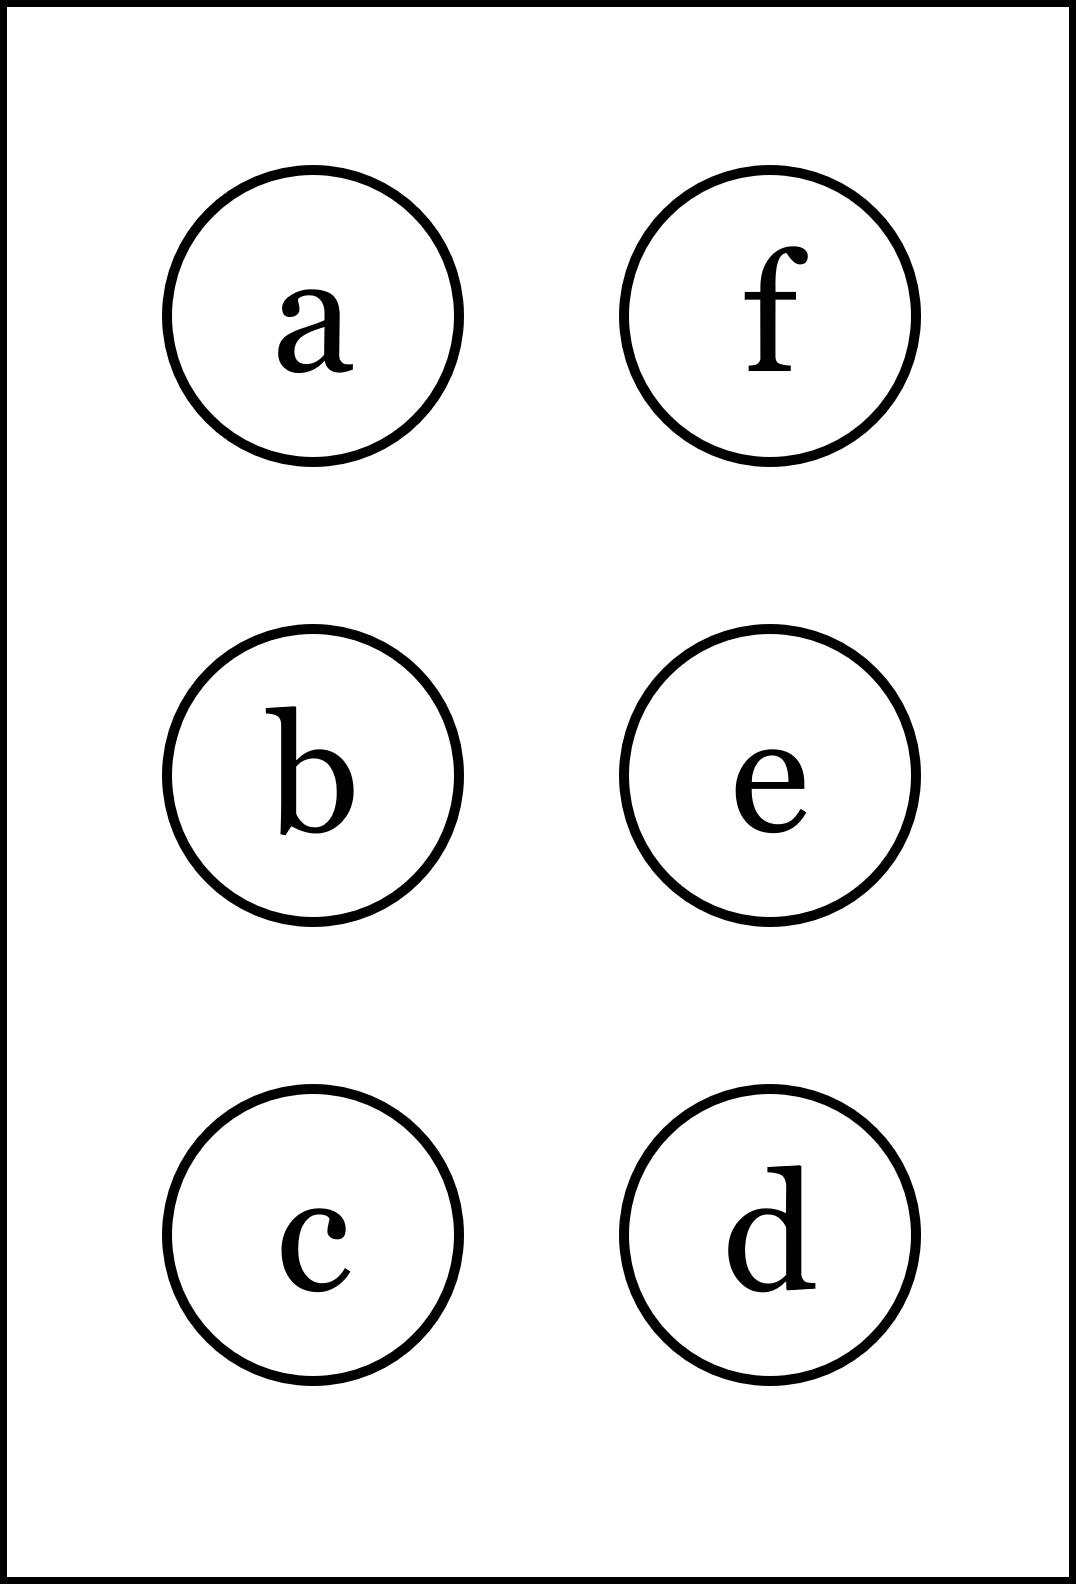
\includegraphics[height=40mm]{../images/braille.png}
{\small Písmeno Braillovej abecedy}
\end{center}
\end{minipage}
\end{center}
\end{minipage}
\\ \hdashline
\begin{minipage}[c][104.5mm][t]{0.5\linewidth}
\begin{center}
\vspace{7mm}
{\huge Tečna funkce, skupina \textit{Eta $\eta$} -\romannumeral3}\\[5mm]
\textit{Meno:}\phantom{xxxxxxxxxxxxxxxxxxxxxxxxxxxxxxxxxxxxxxxxxxxxxxxxxxxxxxxxxxxxxxxxx}\\[5mm]
\begin{minipage}{0.95\linewidth}
\begin{center}
V \textbf{(a)} a \textbf{(b)} urči \text{rovnicu tečny} $y = kx + q$ ku funkci $f(x)$ v bode $x_0$.\\V \textbf{(c)} a \textbf{(d)} urči ypsilonové souřadnice bodů, ve kterých je sklon $f(x)$ rovný $k$.\\Pokud se výsledky shodujú s těmi za otazníky, tak napravo obarvi\\příslušející kroužek načerno. \textbf{Spolu odevzdejte výsledné slovo}.
\end{center}
\end{minipage}
\\[1mm]
\begin{minipage}{0.79\linewidth}
\begin{center}
\begin{varwidth}{\linewidth}
\begin{enumerate}
\small
\item $f(x)=\cfrac{-3x-1}{2x+6}\enspace , \enspace x_0=1$\quad \dotfill\; ???\;\dotfill \quad $y = -\frac{1}{4}x-\frac{1}{8}$
\item $f(x)=-\sqrt{-6x+1}\enspace , \enspace x_0=-\frac{35}{6}$\quad \dotfill\; ???\;\dotfill \quad $y = \frac{1}{2}x-\frac{37}{12}$
\item $f(x)=x^2+5x-6\enspace , \enspace k=-7$\quad \dotfill\; ???\;\dotfill \quad $0$
\item $f(x)=3x^3-9x^2-77x-1\enspace , \enspace k=-5$\quad \dotfill\; ???\;\dotfill \quad $93 , 355$
\item \quad \dotfill\; ???\;\dotfill \quad nebarvi
\item \quad \dotfill\; ???\;\dotfill \quad vybarvi
\end{enumerate}
\end{varwidth}
\end{center}
\end{minipage}
\begin{minipage}{0.20\linewidth}
\begin{center}
{\Huge\bfseries 3.} \\[2mm]
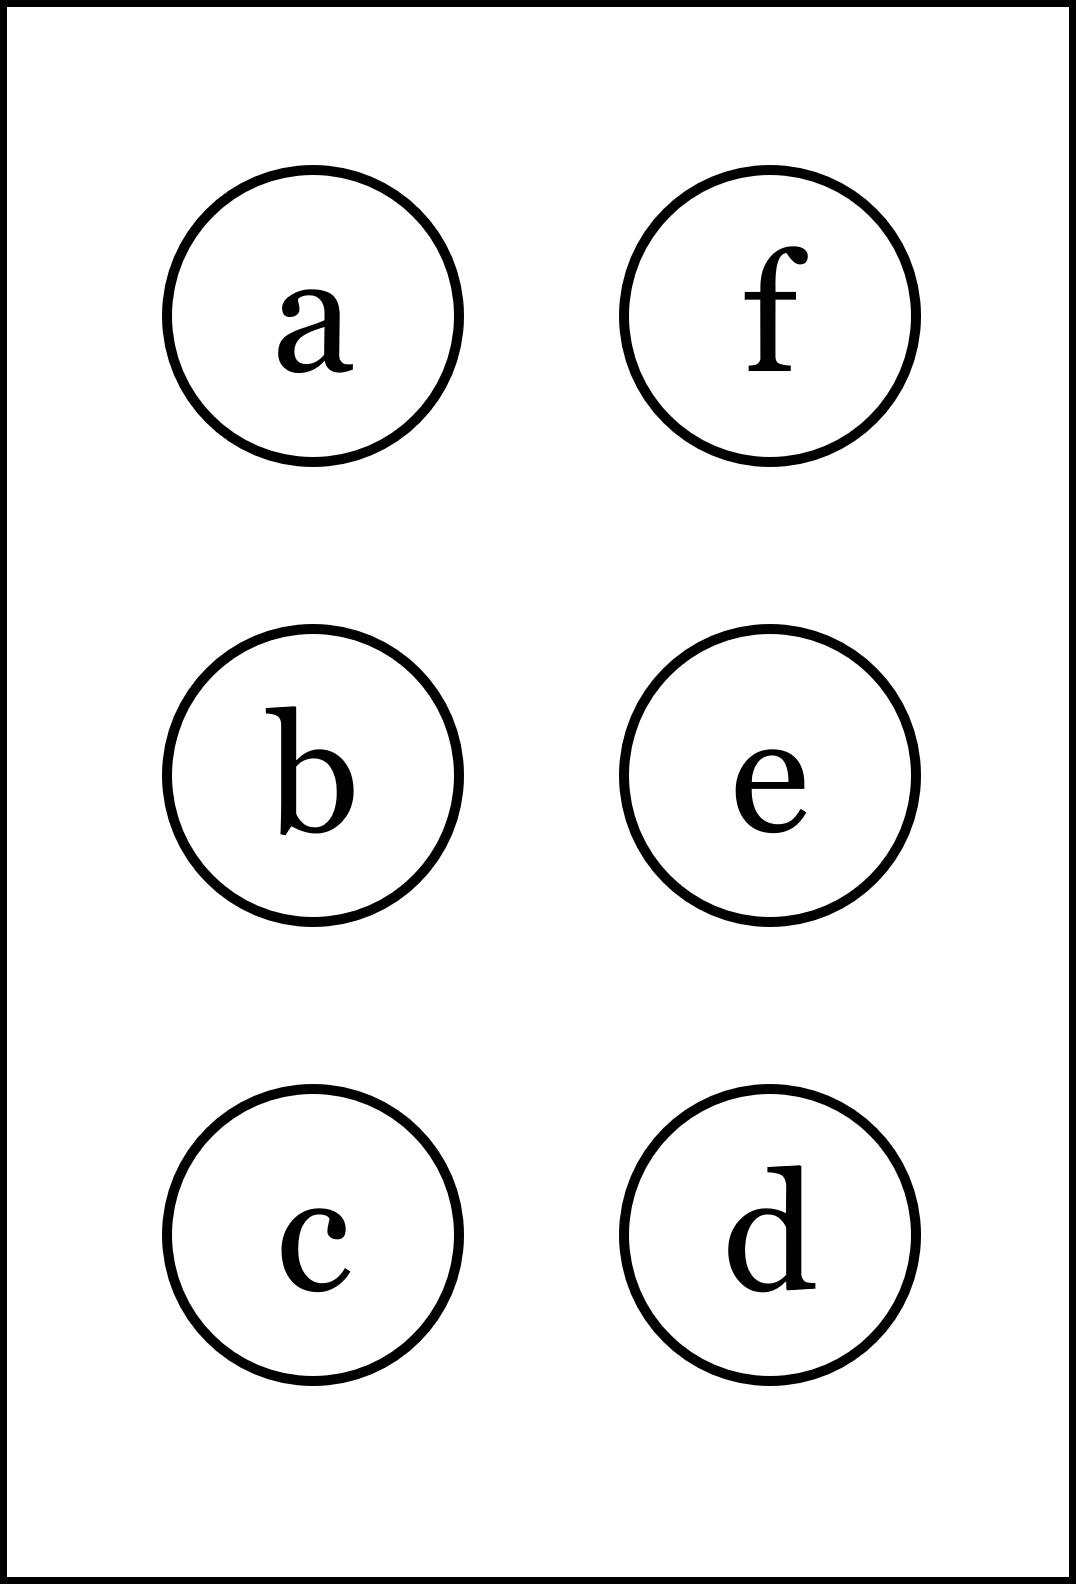
\includegraphics[height=40mm]{../images/braille.png}
{\small Písmeno Braillovej abecedy}
\end{center}
\end{minipage}
\end{center}
\end{minipage}
&
\begin{minipage}[c][104.5mm][t]{0.5\linewidth}
\begin{center}
\vspace{7mm}
{\huge Tečna funkce, skupina \textit{Eta $\eta$} -\romannumeral4}\\[5mm]
\textit{Meno:}\phantom{xxxxxxxxxxxxxxxxxxxxxxxxxxxxxxxxxxxxxxxxxxxxxxxxxxxxxxxxxxxxxxxxx}\\[5mm]
\begin{minipage}{0.95\linewidth}
\begin{center}
V \textbf{(a)} a \textbf{(b)} urči \text{rovnicu tečny} $y = kx + q$ ku funkci $f(x)$ v bode $x_0$.\\V \textbf{(c)} a \textbf{(d)} urči ypsilonové souřadnice bodů, ve kterých je sklon $f(x)$ rovný $k$.\\Pokud se výsledky shodujú s těmi za otazníky, tak napravo obarvi\\příslušející kroužek načerno. \textbf{Spolu odevzdejte výsledné slovo}.
\end{center}
\end{minipage}
\\[1mm]
\begin{minipage}{0.79\linewidth}
\begin{center}
\begin{varwidth}{\linewidth}
\begin{enumerate}
\small
\item $f(x)=\cfrac{-4x+6}{x-8}\enspace , \enspace x_0=3$\quad \dotfill\; ???\;\dotfill \quad $y = \frac{26}{25}x-\frac{24}{5}$
\item $f(x)=-5\sqrt{4x-3}\enspace , \enspace x_0=\frac{7}{4}$\quad \dotfill\; ???\;\dotfill \quad $y = -5x-\frac{5}{4}$
\item $f(x)=-4x^2+4x-1\enspace , \enspace k=1$\quad \dotfill\; ???\;\dotfill \quad $-\frac{1}{16}$
\item $f(x)=2x^3-6x^2-52x-2\enspace , \enspace k=-4$\quad \dotfill\; ???\;\dotfill \quad $62 , 238$
\item \quad \dotfill\; ???\;\dotfill \quad vybarvi
\item \quad \dotfill\; ???\;\dotfill \quad vybarvi
\end{enumerate}
\end{varwidth}
\end{center}
\end{minipage}
\begin{minipage}{0.20\linewidth}
\begin{center}
{\Huge\bfseries 4.} \\[2mm]
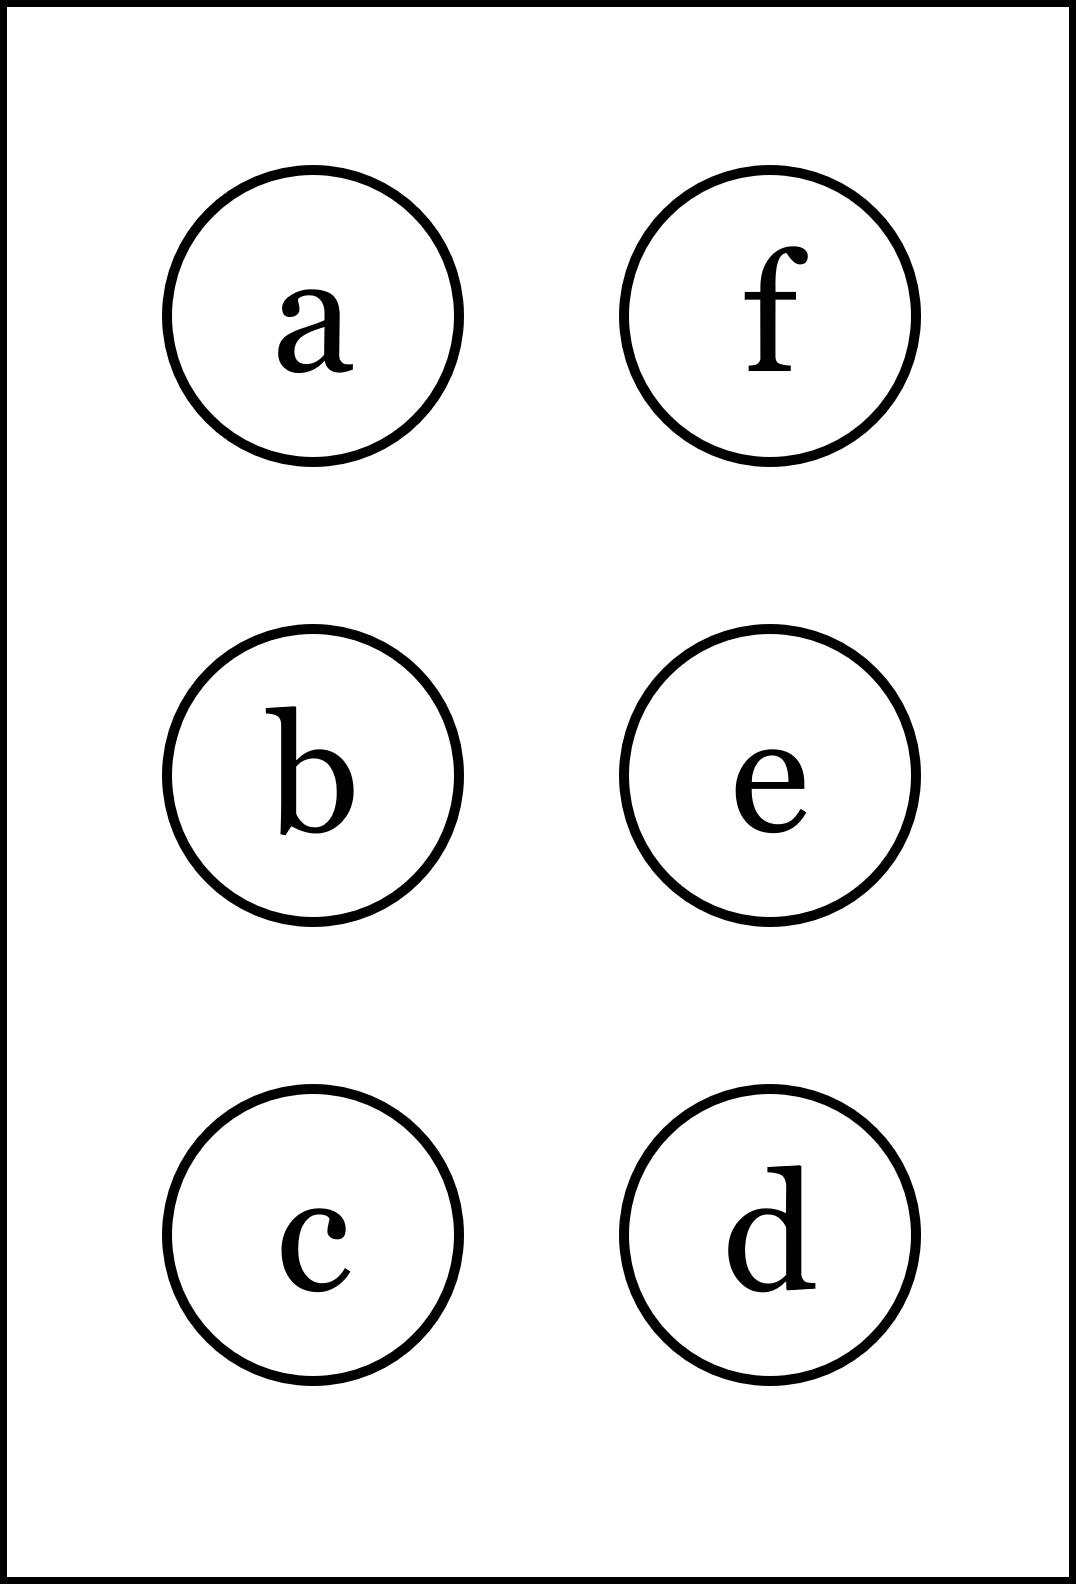
\includegraphics[height=40mm]{../images/braille.png}
{\small Písmeno Braillovej abecedy}
\end{center}
\end{minipage}
\end{center}
\end{minipage}
%
\end{tabular}
\newpage
\thispagestyle{empty}
\begin{tabular}{c:c}
\begin{minipage}[c][104.5mm][t]{0.5\linewidth}
\begin{center}
\vspace{7mm}
{\huge Tečna funkce, skupina \textit{Theta $\theta$} -\romannumeral1}\\[5mm]
\textit{Meno:}\phantom{xxxxxxxxxxxxxxxxxxxxxxxxxxxxxxxxxxxxxxxxxxxxxxxxxxxxxxxxxxxxxxxxx}\\[5mm]
\begin{minipage}{0.95\linewidth}
\begin{center}
V \textbf{(a)} a \textbf{(b)} urči \text{rovnicu tečny} $y = kx + q$ ku funkci $f(x)$ v bode $x_0$.\\V \textbf{(c)} a \textbf{(d)} urči ypsilonové souřadnice bodů, ve kterých je sklon $f(x)$ rovný $k$.\\Pokud se výsledky shodujú s těmi za otazníky, tak napravo obarvi\\příslušející kroužek načerno. \textbf{Spolu odevzdejte výsledné slovo}.
\end{center}
\end{minipage}
\\[1mm]
\begin{minipage}{0.79\linewidth}
\begin{center}
\begin{varwidth}{\linewidth}
\begin{enumerate}
\small
\item $f(x)=\cfrac{4x-4}{-x+8}\enspace , \enspace x_0=2$\quad \dotfill\; ???\;\dotfill \quad $y = \frac{7}{9}x-\frac{8}{9}$
\item $f(x)=5\sqrt{x-3}\enspace , \enspace x_0=4$\quad \dotfill\; ???\;\dotfill \quad $y = \frac{5}{2}x-10$
\item $f(x)=-3x^2+x-1\enspace , \enspace k=-3$\quad \dotfill\; ???\;\dotfill \quad $\frac{1}{3}$
\item $f(x)=x^3+3x^2-10x+1\enspace , \enspace k=-1$\quad \dotfill\; ???\;\dotfill \quad $31 , -5$
\item \quad \dotfill\; ???\;\dotfill \quad vybarvi
\item \quad \dotfill\; ???\;\dotfill \quad nebarvi
\end{enumerate}
\end{varwidth}
\end{center}
\end{minipage}
\begin{minipage}{0.20\linewidth}
\begin{center}
{\Huge\bfseries 1.} \\[2mm]
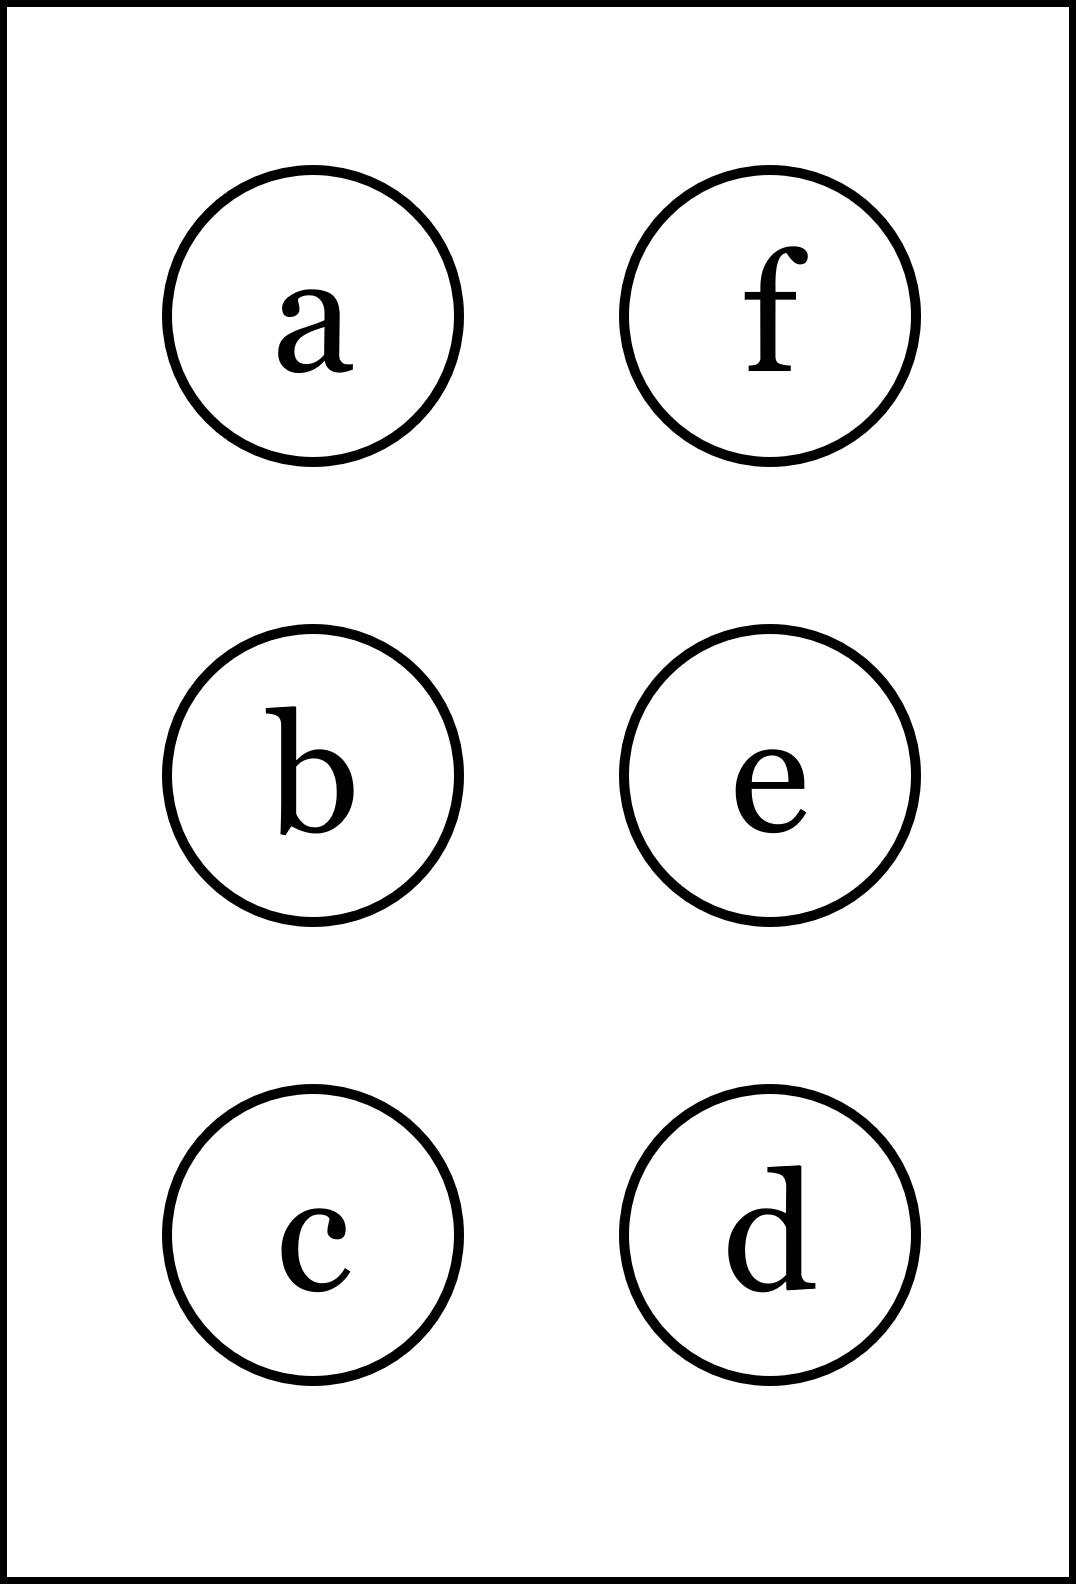
\includegraphics[height=40mm]{../images/braille.png}
{\small Písmeno Braillovej abecedy}
\end{center}
\end{minipage}
\end{center}
\end{minipage}
&
\begin{minipage}[c][104.5mm][t]{0.5\linewidth}
\begin{center}
\vspace{7mm}
{\huge Tečna funkce, skupina \textit{Theta $\theta$} -\romannumeral2}\\[5mm]
\textit{Meno:}\phantom{xxxxxxxxxxxxxxxxxxxxxxxxxxxxxxxxxxxxxxxxxxxxxxxxxxxxxxxxxxxxxxxxx}\\[5mm]
\begin{minipage}{0.95\linewidth}
\begin{center}
V \textbf{(a)} a \textbf{(b)} urči \text{rovnicu tečny} $y = kx + q$ ku funkci $f(x)$ v bode $x_0$.\\V \textbf{(c)} a \textbf{(d)} urči ypsilonové souřadnice bodů, ve kterých je sklon $f(x)$ rovný $k$.\\Pokud se výsledky shodujú s těmi za otazníky, tak napravo obarvi\\příslušející kroužek načerno. \textbf{Spolu odevzdejte výsledné slovo}.
\end{center}
\end{minipage}
\\[1mm]
\begin{minipage}{0.79\linewidth}
\begin{center}
\begin{varwidth}{\linewidth}
\begin{enumerate}
\small
\item $f(x)=\cfrac{8x+1}{x-6}\enspace , \enspace x_0=-1$\quad \dotfill\; ???\;\dotfill \quad $y = -x+0$
\item $f(x)=-7\sqrt{3x-5}\enspace , \enspace x_0=2$\quad \dotfill\; ???\;\dotfill \quad $y = -\frac{21}{2}x+28$
\item $f(x)=4x^2+7x+3\enspace , \enspace k=-3$\quad \dotfill\; ???\;\dotfill \quad $-\frac{11}{2}$
\item $f(x)=x^3-3x^2-48x-5\enspace , \enspace k=-3$\quad \dotfill\; ???\;\dotfill \quad $85 , -195$
\item \quad \dotfill\; ???\;\dotfill \quad nebarvi
\item \quad \dotfill\; ???\;\dotfill \quad nebarvi
\end{enumerate}
\end{varwidth}
\end{center}
\end{minipage}
\begin{minipage}{0.20\linewidth}
\begin{center}
{\Huge\bfseries 2.} \\[2mm]
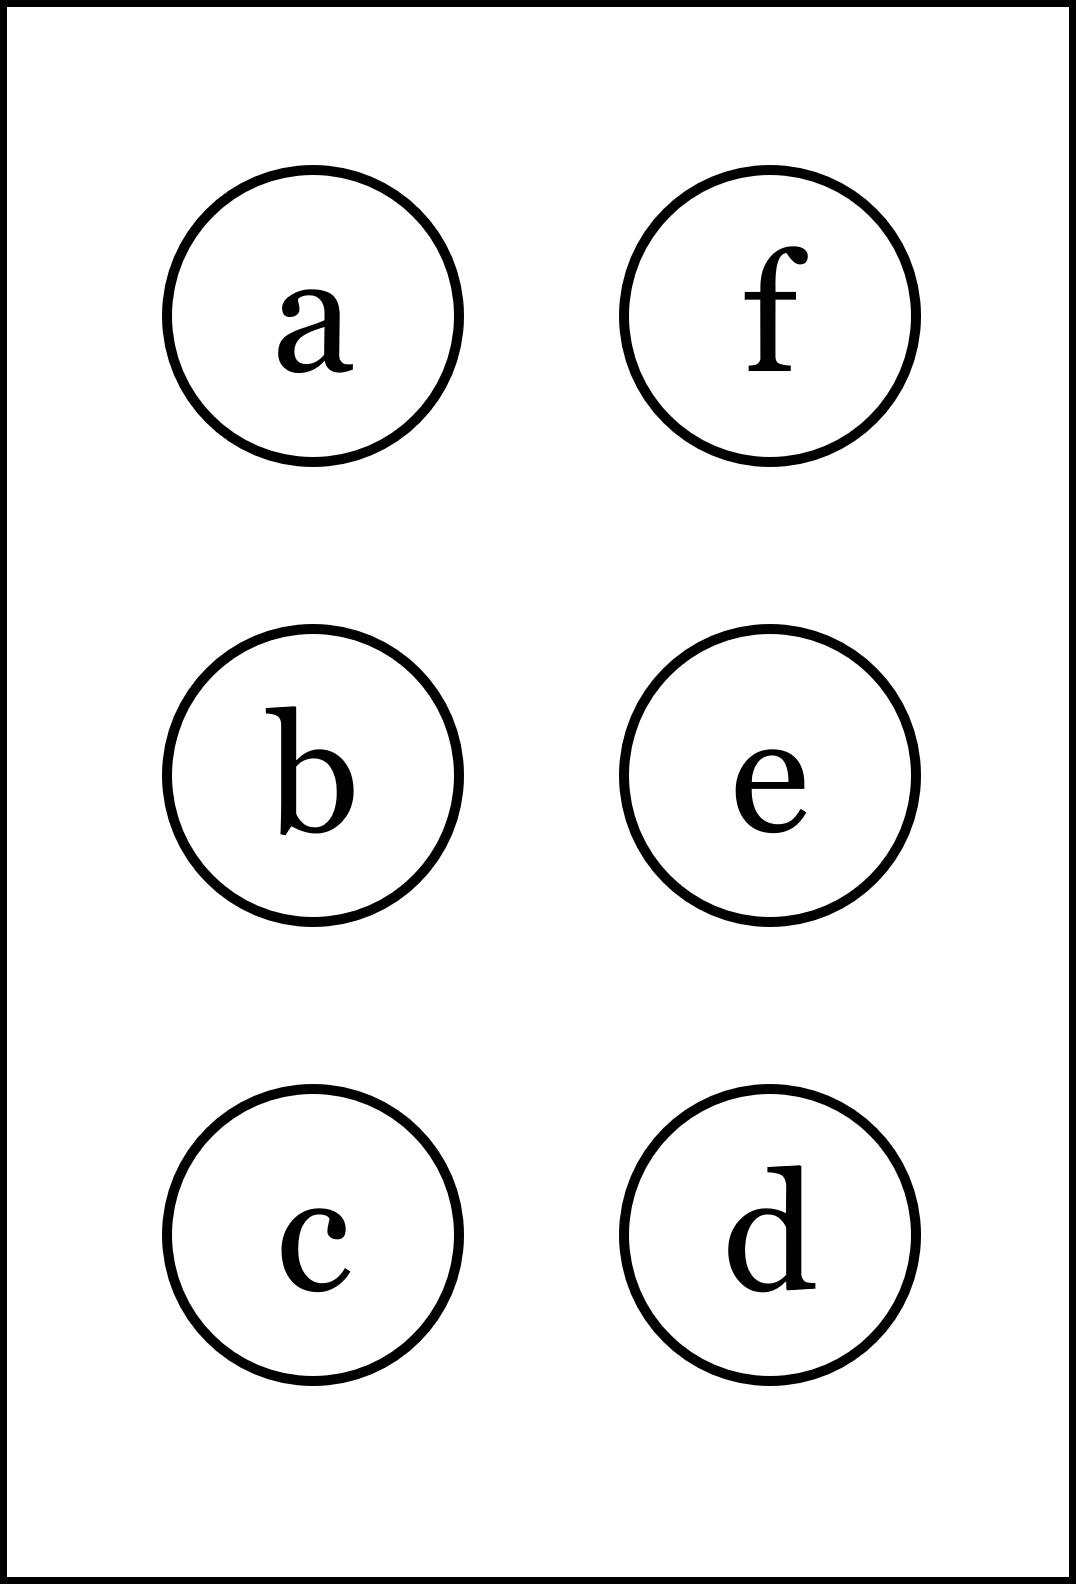
\includegraphics[height=40mm]{../images/braille.png}
{\small Písmeno Braillovej abecedy}
\end{center}
\end{minipage}
\end{center}
\end{minipage}
\\ \hdashline
\begin{minipage}[c][104.5mm][t]{0.5\linewidth}
\begin{center}
\vspace{7mm}
{\huge Tečna funkce, skupina \textit{Theta $\theta$} -\romannumeral3}\\[5mm]
\textit{Meno:}\phantom{xxxxxxxxxxxxxxxxxxxxxxxxxxxxxxxxxxxxxxxxxxxxxxxxxxxxxxxxxxxxxxxxx}\\[5mm]
\begin{minipage}{0.95\linewidth}
\begin{center}
V \textbf{(a)} a \textbf{(b)} urči \text{rovnicu tečny} $y = kx + q$ ku funkci $f(x)$ v bode $x_0$.\\V \textbf{(c)} a \textbf{(d)} urči ypsilonové souřadnice bodů, ve kterých je sklon $f(x)$ rovný $k$.\\Pokud se výsledky shodujú s těmi za otazníky, tak napravo obarvi\\příslušející kroužek načerno. \textbf{Spolu odevzdejte výsledné slovo}.
\end{center}
\end{minipage}
\\[1mm]
\begin{minipage}{0.79\linewidth}
\begin{center}
\begin{varwidth}{\linewidth}
\begin{enumerate}
\small
\item $f(x)=\cfrac{-x-1}{3x-1}\enspace , \enspace x_0=1$\quad \dotfill\; ???\;\dotfill \quad $y = x-2$
\item $f(x)=-8\sqrt{3x+4}\enspace , \enspace x_0=-1$\quad \dotfill\; ???\;\dotfill \quad $y = -12x-20$
\item $f(x)=5x^2+2x+3\enspace , \enspace k=1$\quad \dotfill\; ???\;\dotfill \quad $\frac{57}{20}$
\item $f(x)=x^3-6x^2-14x+2\enspace , \enspace k=1$\quad \dotfill\; ???\;\dotfill \quad $9 , 47$
\item \quad \dotfill\; ???\;\dotfill \quad nebarvi
\item \quad \dotfill\; ???\;\dotfill \quad nebarvi
\end{enumerate}
\end{varwidth}
\end{center}
\end{minipage}
\begin{minipage}{0.20\linewidth}
\begin{center}
{\Huge\bfseries 3.} \\[2mm]
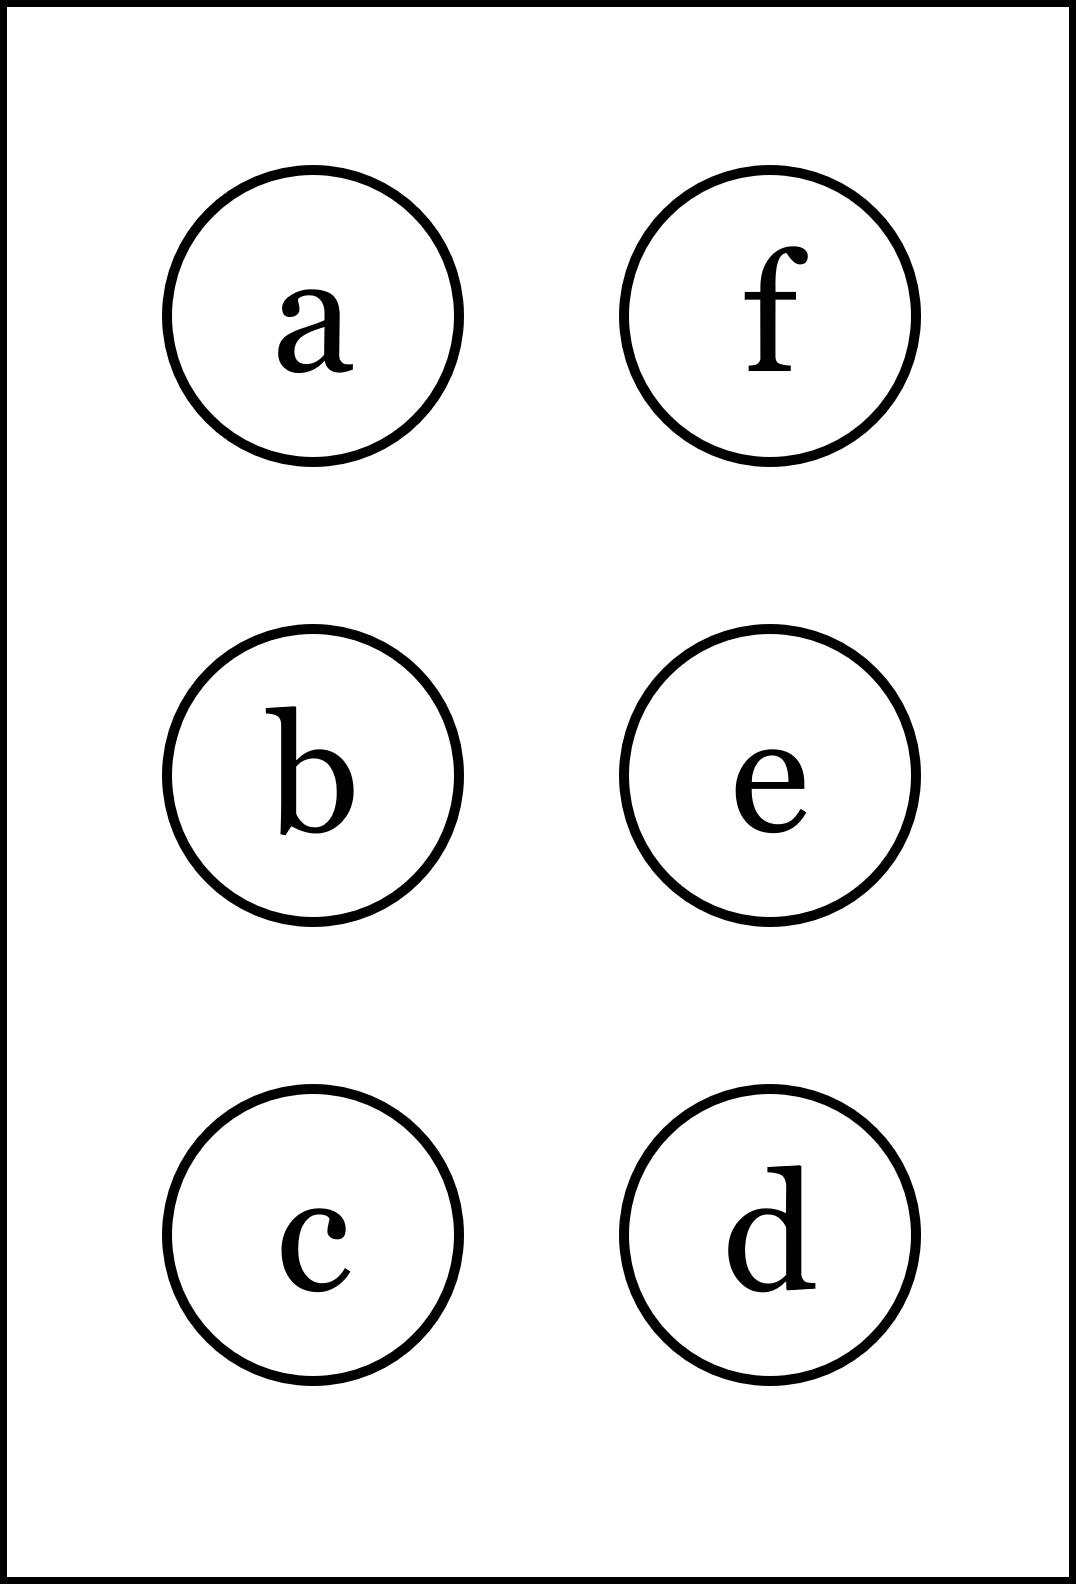
\includegraphics[height=40mm]{../images/braille.png}
{\small Písmeno Braillovej abecedy}
\end{center}
\end{minipage}
\end{center}
\end{minipage}
&
\begin{minipage}[c][104.5mm][t]{0.5\linewidth}
\begin{center}
\vspace{7mm}
{\huge Tečna funkce, skupina \textit{Theta $\theta$} -\romannumeral4}\\[5mm]
\textit{Meno:}\phantom{xxxxxxxxxxxxxxxxxxxxxxxxxxxxxxxxxxxxxxxxxxxxxxxxxxxxxxxxxxxxxxxxx}\\[5mm]
\begin{minipage}{0.95\linewidth}
\begin{center}
V \textbf{(a)} a \textbf{(b)} urči \text{rovnicu tečny} $y = kx + q$ ku funkci $f(x)$ v bode $x_0$.\\V \textbf{(c)} a \textbf{(d)} urči ypsilonové souřadnice bodů, ve kterých je sklon $f(x)$ rovný $k$.\\Pokud se výsledky shodujú s těmi za otazníky, tak napravo obarvi\\příslušející kroužek načerno. \textbf{Spolu odevzdejte výsledné slovo}.
\end{center}
\end{minipage}
\\[1mm]
\begin{minipage}{0.79\linewidth}
\begin{center}
\begin{varwidth}{\linewidth}
\begin{enumerate}
\small
\item $f(x)=\cfrac{-3x+5}{-2x-2}\enspace , \enspace x_0=-3$\quad \dotfill\; ???\;\dotfill \quad $y = x+\frac{13}{2}$
\item $f(x)=4\sqrt{3x-5}\enspace , \enspace x_0=\frac{41}{3}$\quad \dotfill\; ???\;\dotfill \quad $y = x+\frac{62}{3}$
\item $f(x)=3x^2+3x-4\enspace , \enspace k=3$\quad \dotfill\; ???\;\dotfill \quad $4$
\item $f(x)=x^3-9x^2+13x+1\enspace , \enspace k=-2$\quad \dotfill\; ???\;\dotfill \quad $6 , -164$
\item \quad \dotfill\; ???\;\dotfill \quad nebarvi
\item \quad \dotfill\; ???\;\dotfill \quad nebarvi
\end{enumerate}
\end{varwidth}
\end{center}
\end{minipage}
\begin{minipage}{0.20\linewidth}
\begin{center}
{\Huge\bfseries 4.} \\[2mm]
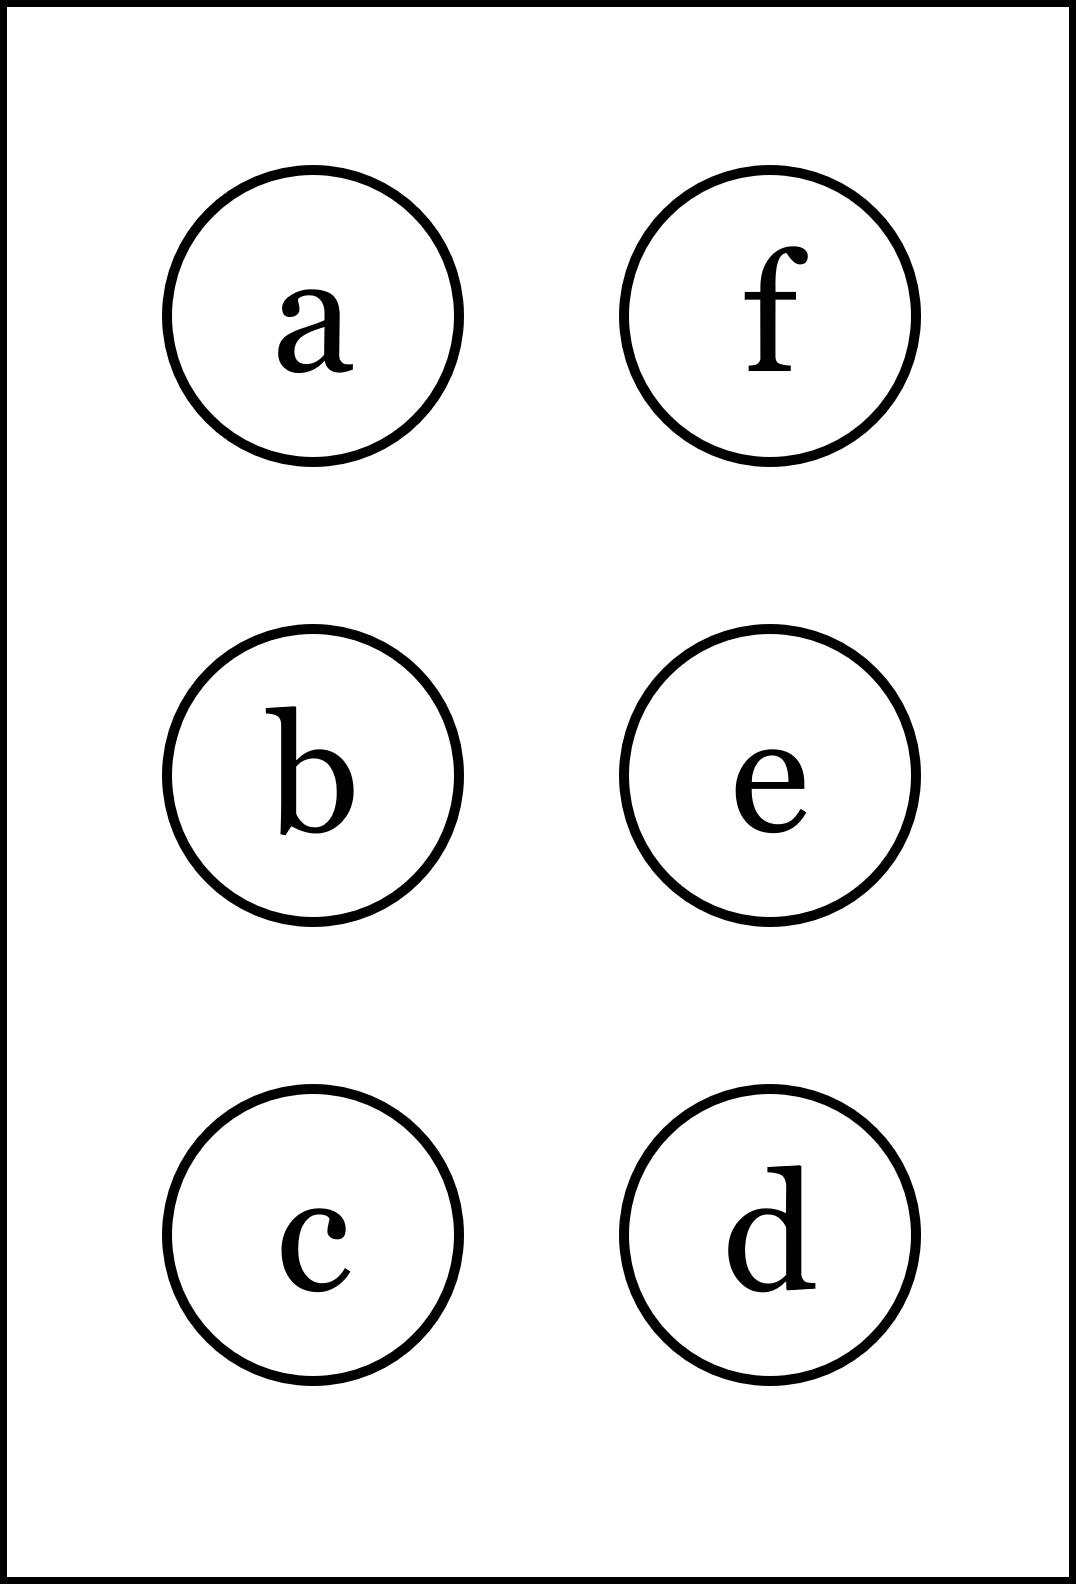
\includegraphics[height=40mm]{../images/braille.png}
{\small Písmeno Braillovej abecedy}
\end{center}
\end{minipage}
\end{center}
\end{minipage}
%
\end{tabular}
\newpage
\thispagestyle{empty}
\begin{tabular}{c:c}
\begin{minipage}[c][104.5mm][t]{0.5\linewidth}
\begin{center}
\vspace{7mm}
{\huge Tečna funkce, skupina \textit{Iota $\iota$} -\romannumeral1}\\[5mm]
\textit{Meno:}\phantom{xxxxxxxxxxxxxxxxxxxxxxxxxxxxxxxxxxxxxxxxxxxxxxxxxxxxxxxxxxxxxxxxx}\\[5mm]
\begin{minipage}{0.95\linewidth}
\begin{center}
V \textbf{(a)} a \textbf{(b)} urči \text{rovnicu tečny} $y = kx + q$ ku funkci $f(x)$ v bode $x_0$.\\V \textbf{(c)} a \textbf{(d)} urči ypsilonové souřadnice bodů, ve kterých je sklon $f(x)$ rovný $k$.\\Pokud se výsledky shodujú s těmi za otazníky, tak napravo obarvi\\příslušející kroužek načerno. \textbf{Spolu odevzdejte výsledné slovo}.
\end{center}
\end{minipage}
\\[1mm]
\begin{minipage}{0.79\linewidth}
\begin{center}
\begin{varwidth}{\linewidth}
\begin{enumerate}
\small
\item $f(x)=\cfrac{-5x+8}{-3x+1}\enspace , \enspace x_0=2$\quad \dotfill\; ???\;\dotfill \quad $y = \frac{19}{25}x-\frac{28}{25}$
\item $f(x)=6\sqrt{-x+4}\enspace , \enspace x_0=-12$\quad \dotfill\; ???\;\dotfill \quad $y = -\frac{3}{4}x+30$
\item $f(x)=-x^2-8x-1\enspace , \enspace k=-3$\quad \dotfill\; ???\;\dotfill \quad $\frac{59}{4}$
\item $f(x)=x^3-9x^2+23x-1\enspace , \enspace k=-1$\quad \dotfill\; ???\;\dotfill \quad $17 , 11$
\item \quad \dotfill\; ???\;\dotfill \quad nebarvi
\item \quad \dotfill\; ???\;\dotfill \quad vybarvi
\end{enumerate}
\end{varwidth}
\end{center}
\end{minipage}
\begin{minipage}{0.20\linewidth}
\begin{center}
{\Huge\bfseries 1.} \\[2mm]
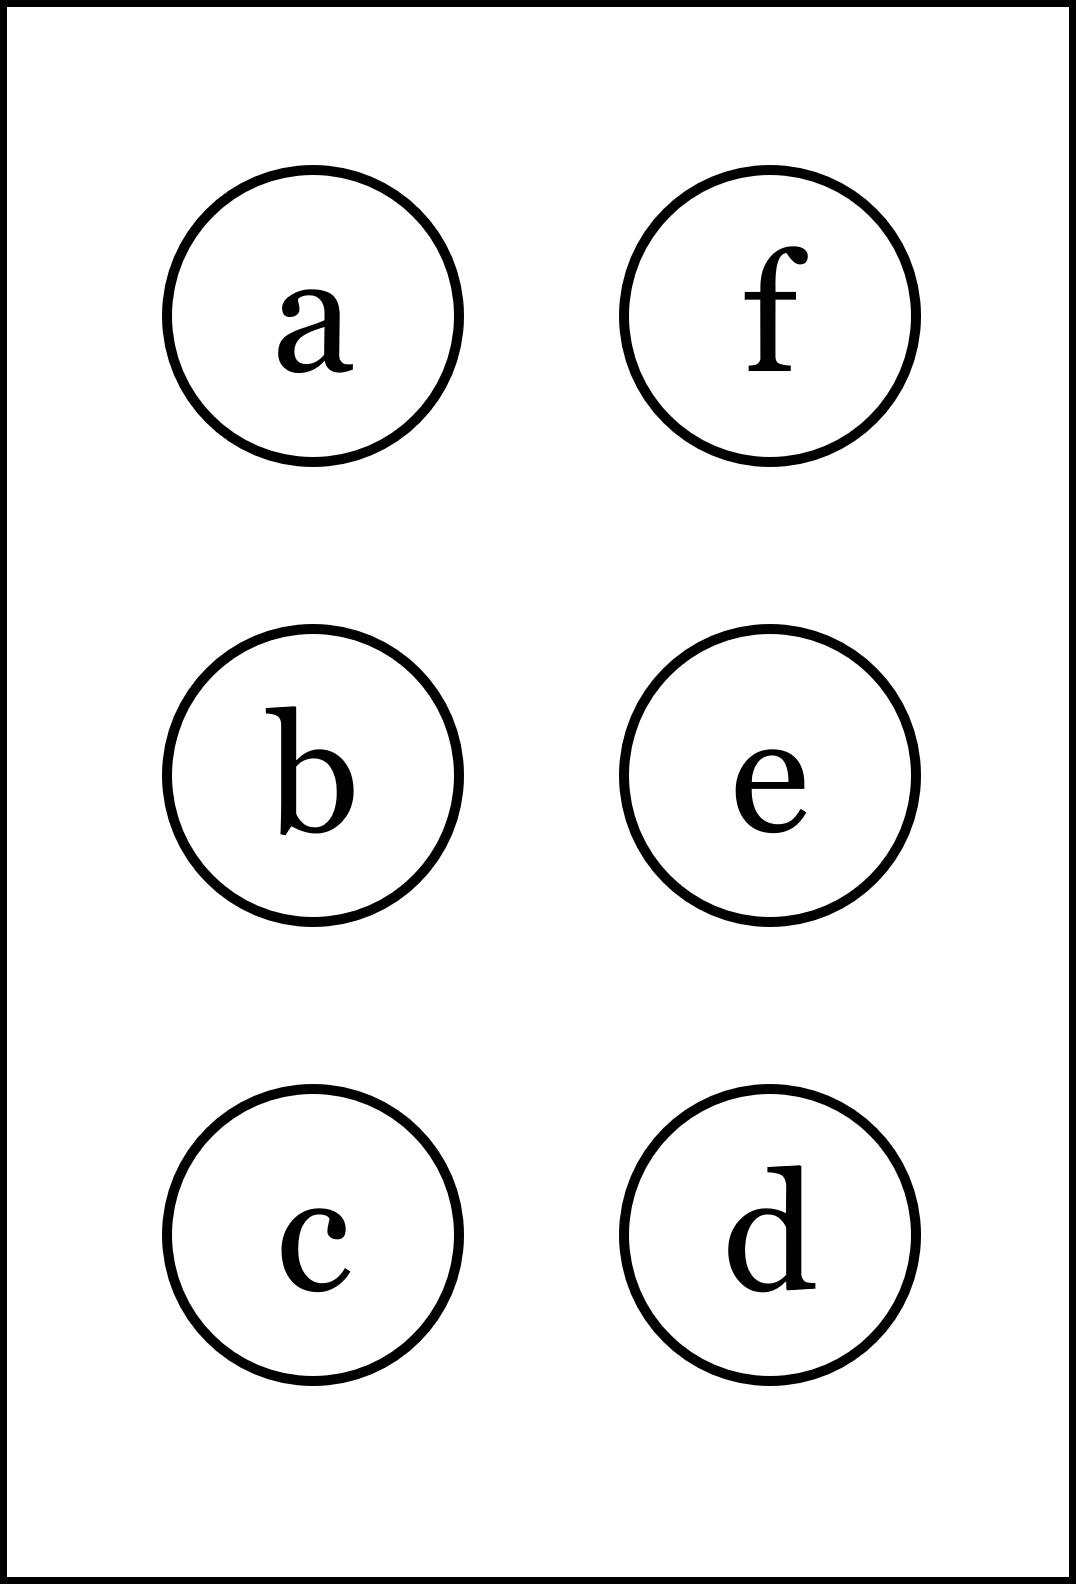
\includegraphics[height=40mm]{../images/braille.png}
{\small Písmeno Braillovej abecedy}
\end{center}
\end{minipage}
\end{center}
\end{minipage}
&
\begin{minipage}[c][104.5mm][t]{0.5\linewidth}
\begin{center}
\vspace{7mm}
{\huge Tečna funkce, skupina \textit{Iota $\iota$} -\romannumeral2}\\[5mm]
\textit{Meno:}\phantom{xxxxxxxxxxxxxxxxxxxxxxxxxxxxxxxxxxxxxxxxxxxxxxxxxxxxxxxxxxxxxxxxx}\\[5mm]
\begin{minipage}{0.95\linewidth}
\begin{center}
V \textbf{(a)} a \textbf{(b)} urči \text{rovnicu tečny} $y = kx + q$ ku funkci $f(x)$ v bode $x_0$.\\V \textbf{(c)} a \textbf{(d)} urči ypsilonové souřadnice bodů, ve kterých je sklon $f(x)$ rovný $k$.\\Pokud se výsledky shodujú s těmi za otazníky, tak napravo obarvi\\příslušející kroužek načerno. \textbf{Spolu odevzdejte výsledné slovo}.
\end{center}
\end{minipage}
\\[1mm]
\begin{minipage}{0.79\linewidth}
\begin{center}
\begin{varwidth}{\linewidth}
\begin{enumerate}
\small
\item $f(x)=\cfrac{-4x-1}{x-3}\enspace , \enspace x_0=4$\quad \dotfill\; ???\;\dotfill \quad $y = 13x-69$
\item $f(x)=-2\sqrt{-6x-6}\enspace , \enspace x_0=-\frac{35}{3}$\quad \dotfill\; ???\;\dotfill \quad $y = \frac{3}{4}x-\frac{29}{2}$
\item $f(x)=-5x^2-7x+9\enspace , \enspace k=7$\quad \dotfill\; ???\;\dotfill \quad $9$
\item $f(x)=x^3-6x^2-37x-4\enspace , \enspace k=-1$\quad \dotfill\; ???\;\dotfill \quad $38 , 218$
\item \quad \dotfill\; ???\;\dotfill \quad vybarvi
\item \quad \dotfill\; ???\;\dotfill \quad nebarvi
\end{enumerate}
\end{varwidth}
\end{center}
\end{minipage}
\begin{minipage}{0.20\linewidth}
\begin{center}
{\Huge\bfseries 2.} \\[2mm]
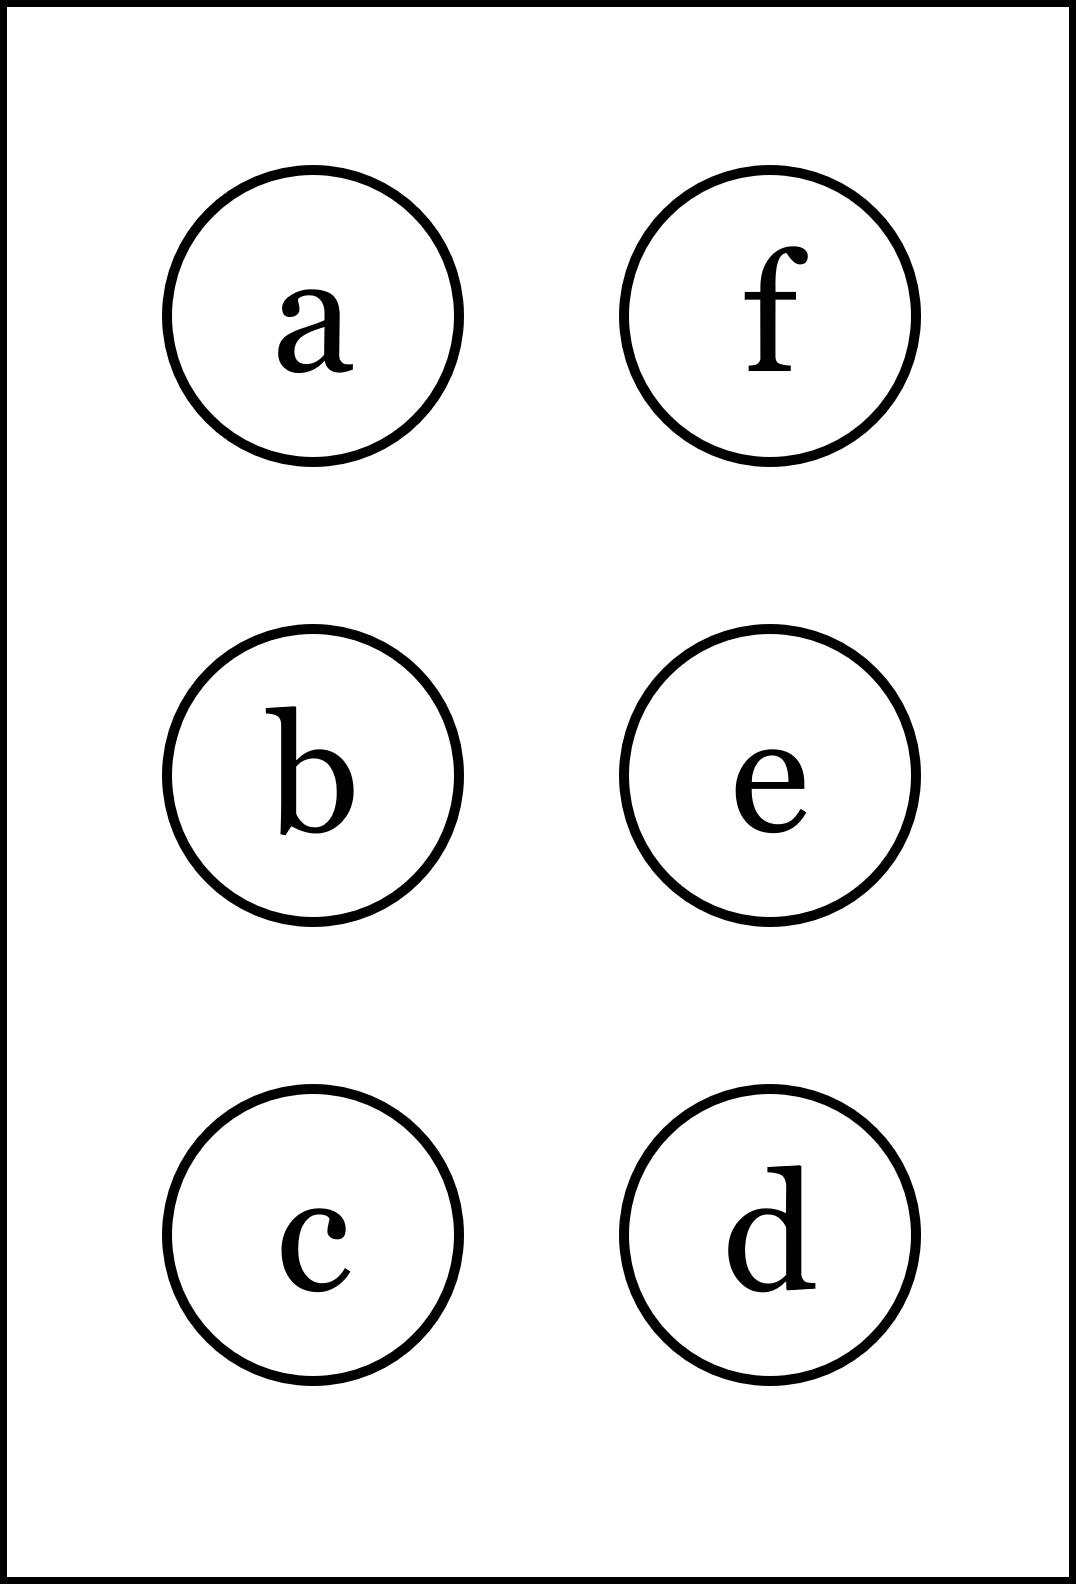
\includegraphics[height=40mm]{../images/braille.png}
{\small Písmeno Braillovej abecedy}
\end{center}
\end{minipage}
\end{center}
\end{minipage}
\\ \hdashline
\begin{minipage}[c][104.5mm][t]{0.5\linewidth}
\begin{center}
\vspace{7mm}
{\huge Tečna funkce, skupina \textit{Iota $\iota$} -\romannumeral3}\\[5mm]
\textit{Meno:}\phantom{xxxxxxxxxxxxxxxxxxxxxxxxxxxxxxxxxxxxxxxxxxxxxxxxxxxxxxxxxxxxxxxxx}\\[5mm]
\begin{minipage}{0.95\linewidth}
\begin{center}
V \textbf{(a)} a \textbf{(b)} urči \text{rovnicu tečny} $y = kx + q$ ku funkci $f(x)$ v bode $x_0$.\\V \textbf{(c)} a \textbf{(d)} urči ypsilonové souřadnice bodů, ve kterých je sklon $f(x)$ rovný $k$.\\Pokud se výsledky shodujú s těmi za otazníky, tak napravo obarvi\\příslušející kroužek načerno. \textbf{Spolu odevzdejte výsledné slovo}.
\end{center}
\end{minipage}
\\[1mm]
\begin{minipage}{0.79\linewidth}
\begin{center}
\begin{varwidth}{\linewidth}
\begin{enumerate}
\small
\item $f(x)=\cfrac{-x+9}{7x-7}\enspace , \enspace x_0=-1$\quad \dotfill\; ???\;\dotfill \quad $y = -\frac{2}{7}x-1$
\item $f(x)=3\sqrt{x+3}\enspace , \enspace x_0=13$\quad \dotfill\; ???\;\dotfill \quad $y = \frac{3}{8}x+\frac{57}{4}$
\item $f(x)=5x^2-4x-3\enspace , \enspace k=2$\quad \dotfill\; ???\;\dotfill \quad $-\frac{18}{5}$
\item $f(x)=3x^3-9x^2-30x-2\enspace , \enspace k=-3$\quad \dotfill\; ???\;\dotfill \quad $16 , 88$
\item \quad \dotfill\; ???\;\dotfill \quad nebarvi
\item \quad \dotfill\; ???\;\dotfill \quad nebarvi
\end{enumerate}
\end{varwidth}
\end{center}
\end{minipage}
\begin{minipage}{0.20\linewidth}
\begin{center}
{\Huge\bfseries 3.} \\[2mm]
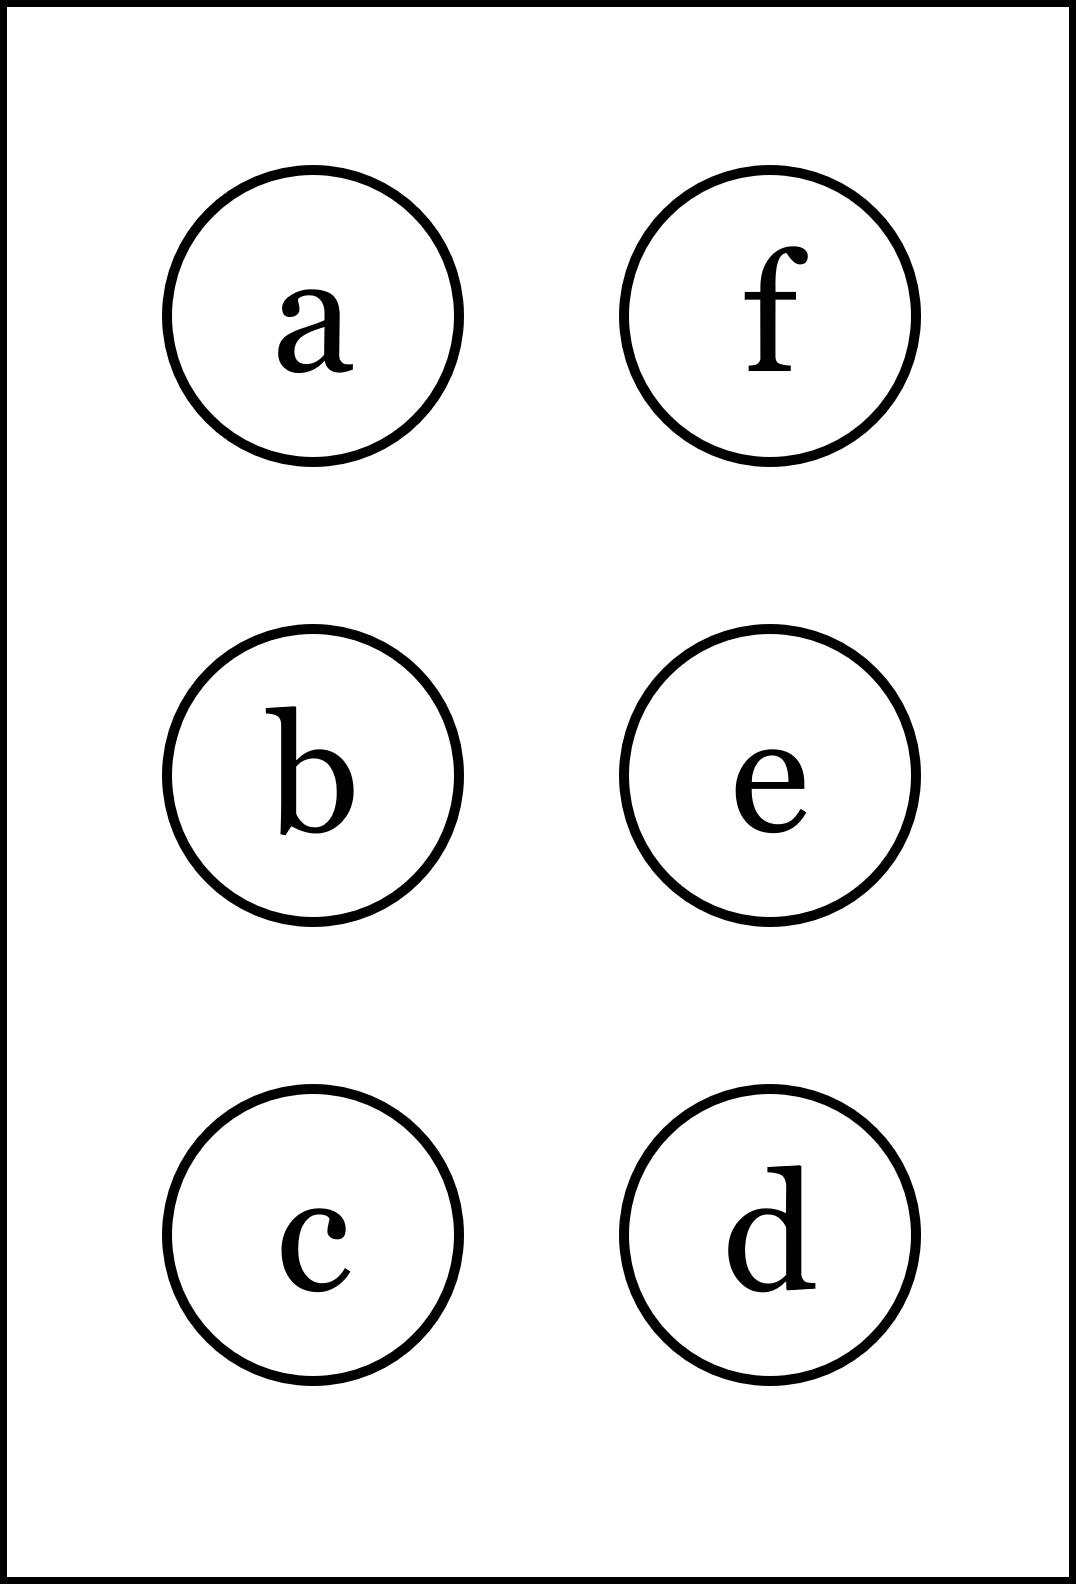
\includegraphics[height=40mm]{../images/braille.png}
{\small Písmeno Braillovej abecedy}
\end{center}
\end{minipage}
\end{center}
\end{minipage}
&
\begin{minipage}[c][104.5mm][t]{0.5\linewidth}
\begin{center}
\vspace{7mm}
{\huge Tečna funkce, skupina \textit{Iota $\iota$} -\romannumeral4}\\[5mm]
\textit{Meno:}\phantom{xxxxxxxxxxxxxxxxxxxxxxxxxxxxxxxxxxxxxxxxxxxxxxxxxxxxxxxxxxxxxxxxx}\\[5mm]
\begin{minipage}{0.95\linewidth}
\begin{center}
V \textbf{(a)} a \textbf{(b)} urči \text{rovnicu tečny} $y = kx + q$ ku funkci $f(x)$ v bode $x_0$.\\V \textbf{(c)} a \textbf{(d)} urči ypsilonové souřadnice bodů, ve kterých je sklon $f(x)$ rovný $k$.\\Pokud se výsledky shodujú s těmi za otazníky, tak napravo obarvi\\příslušející kroužek načerno. \textbf{Spolu odevzdejte výsledné slovo}.
\end{center}
\end{minipage}
\\[1mm]
\begin{minipage}{0.79\linewidth}
\begin{center}
\begin{varwidth}{\linewidth}
\begin{enumerate}
\small
\item $f(x)=\cfrac{-8x-5}{4x-1}\enspace , \enspace x_0=1$\quad \dotfill\; ???\;\dotfill \quad $y = \frac{28}{9}x-\frac{67}{9}$
\item $f(x)=-8\sqrt{-x-1}\enspace , \enspace x_0=-10$\quad \dotfill\; ???\;\dotfill \quad $y = \frac{4}{3}x-\frac{32}{3}$
\item $f(x)=-3x^2-2x+3\enspace , \enspace k=-1$\quad \dotfill\; ???\;\dotfill \quad $\frac{13}{4}$
\item $f(x)=x^3+3x^2-7x+5\enspace , \enspace k=2$\quad \dotfill\; ???\;\dotfill \quad $26 , 16$
\item \quad \dotfill\; ???\;\dotfill \quad nebarvi
\item \quad \dotfill\; ???\;\dotfill \quad nebarvi
\end{enumerate}
\end{varwidth}
\end{center}
\end{minipage}
\begin{minipage}{0.20\linewidth}
\begin{center}
{\Huge\bfseries 4.} \\[2mm]
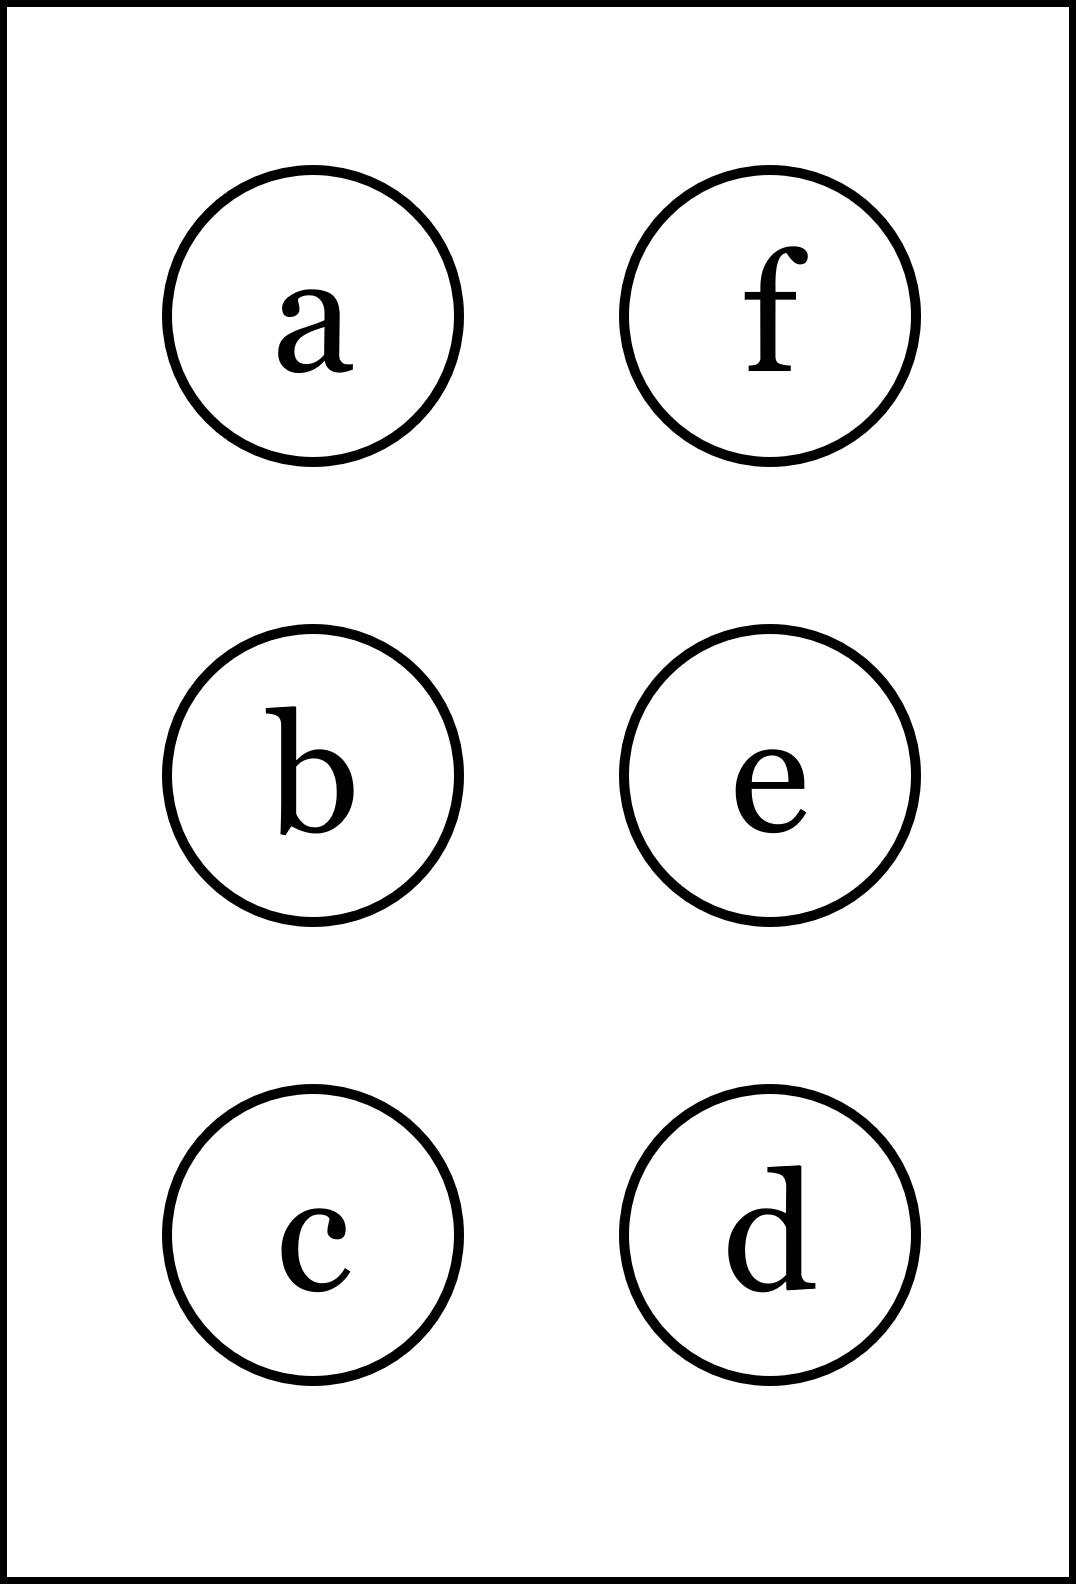
\includegraphics[height=40mm]{../images/braille.png}
{\small Písmeno Braillovej abecedy}
\end{center}
\end{minipage}
\end{center}
\end{minipage}
%
\end{tabular}
\newpage
\thispagestyle{empty}
\begin{tabular}{c:c}
\begin{minipage}[c][104.5mm][t]{0.5\linewidth}
\begin{center}
\vspace{7mm}
{\huge Tečna funkce, skupina \textit{Kappa $\kappa$} -\romannumeral1}\\[5mm]
\textit{Meno:}\phantom{xxxxxxxxxxxxxxxxxxxxxxxxxxxxxxxxxxxxxxxxxxxxxxxxxxxxxxxxxxxxxxxxx}\\[5mm]
\begin{minipage}{0.95\linewidth}
\begin{center}
V \textbf{(a)} a \textbf{(b)} urči \text{rovnicu tečny} $y = kx + q$ ku funkci $f(x)$ v bode $x_0$.\\V \textbf{(c)} a \textbf{(d)} urči ypsilonové souřadnice bodů, ve kterých je sklon $f(x)$ rovný $k$.\\Pokud se výsledky shodujú s těmi za otazníky, tak napravo obarvi\\příslušející kroužek načerno. \textbf{Spolu odevzdejte výsledné slovo}.
\end{center}
\end{minipage}
\\[1mm]
\begin{minipage}{0.79\linewidth}
\begin{center}
\begin{varwidth}{\linewidth}
\begin{enumerate}
\small
\item $f(x)=\cfrac{3x-1}{x+3}\enspace , \enspace x_0=1$\quad \dotfill\; ???\;\dotfill \quad $y = \frac{5}{8}x-\frac{1}{8}$
\item $f(x)=2\sqrt{2x+5}\enspace , \enspace x_0=\frac{11}{2}$\quad \dotfill\; ???\;\dotfill \quad $y = \frac{1}{2}x+\frac{21}{2}$
\item $f(x)=-2x^2-7x-5\enspace , \enspace k=1$\quad \dotfill\; ???\;\dotfill \quad $11$
\item $f(x)=x^3-6x^2-14x+2\enspace , \enspace k=1$\quad \dotfill\; ???\;\dotfill \quad $9 , 47$
\item \quad \dotfill\; ???\;\dotfill \quad nebarvi
\item \quad \dotfill\; ???\;\dotfill \quad vybarvi
\end{enumerate}
\end{varwidth}
\end{center}
\end{minipage}
\begin{minipage}{0.20\linewidth}
\begin{center}
{\Huge\bfseries 1.} \\[2mm]
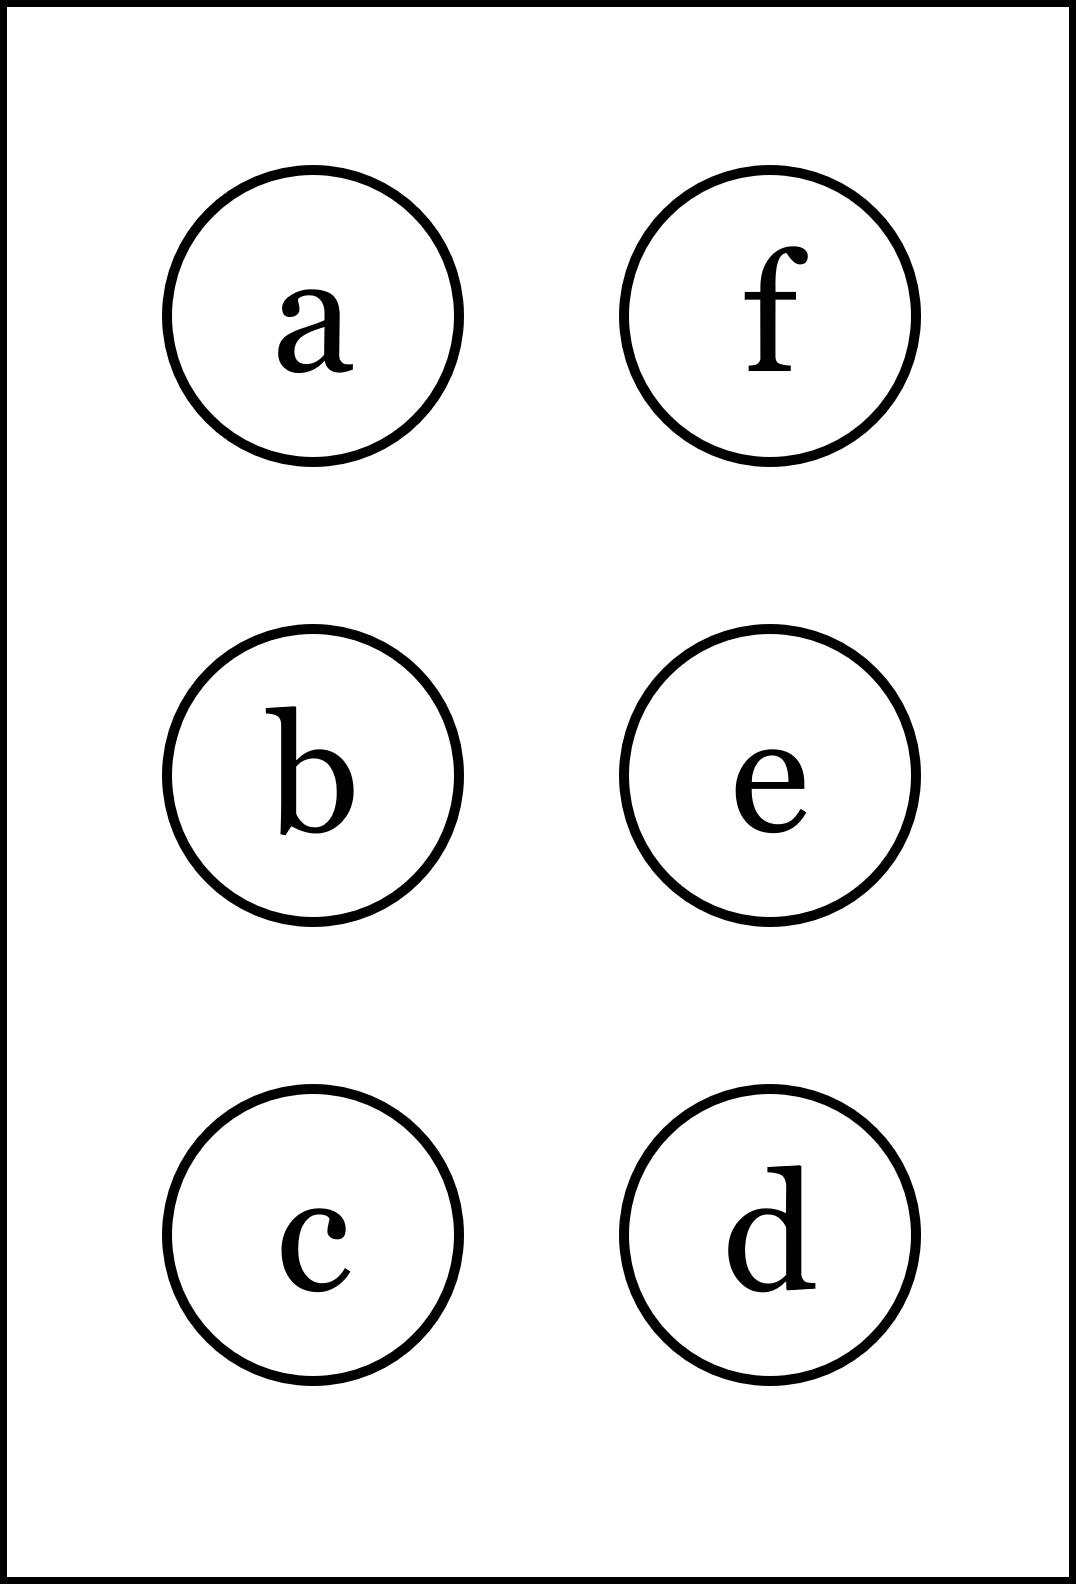
\includegraphics[height=40mm]{../images/braille.png}
{\small Písmeno Braillovej abecedy}
\end{center}
\end{minipage}
\end{center}
\end{minipage}
&
\begin{minipage}[c][104.5mm][t]{0.5\linewidth}
\begin{center}
\vspace{7mm}
{\huge Tečna funkce, skupina \textit{Kappa $\kappa$} -\romannumeral2}\\[5mm]
\textit{Meno:}\phantom{xxxxxxxxxxxxxxxxxxxxxxxxxxxxxxxxxxxxxxxxxxxxxxxxxxxxxxxxxxxxxxxxx}\\[5mm]
\begin{minipage}{0.95\linewidth}
\begin{center}
V \textbf{(a)} a \textbf{(b)} urči \text{rovnicu tečny} $y = kx + q$ ku funkci $f(x)$ v bode $x_0$.\\V \textbf{(c)} a \textbf{(d)} urči ypsilonové souřadnice bodů, ve kterých je sklon $f(x)$ rovný $k$.\\Pokud se výsledky shodujú s těmi za otazníky, tak napravo obarvi\\příslušející kroužek načerno. \textbf{Spolu odevzdejte výsledné slovo}.
\end{center}
\end{minipage}
\\[1mm]
\begin{minipage}{0.79\linewidth}
\begin{center}
\begin{varwidth}{\linewidth}
\begin{enumerate}
\small
\item $f(x)=\cfrac{2x-3}{-5x-2}\enspace , \enspace x_0=2$\quad \dotfill\; ???\;\dotfill \quad $y = -\frac{19}{144}x+\frac{13}{72}$
\item $f(x)=-5\sqrt{-x+4}\enspace , \enspace x_0=-60$\quad \dotfill\; ???\;\dotfill \quad $y = \frac{5}{16}x-\frac{85}{2}$
\item $f(x)=-4x^2-3x+1\enspace , \enspace k=-2$\quad \dotfill\; ???\;\dotfill \quad $\frac{21}{16}$
\item $f(x)=5x^3-30x^2-77x-3\enspace , \enspace k=-2$\quad \dotfill\; ???\;\dotfill \quad $39 , 257$
\item \quad \dotfill\; ???\;\dotfill \quad vybarvi
\item \quad \dotfill\; ???\;\dotfill \quad nebarvi
\end{enumerate}
\end{varwidth}
\end{center}
\end{minipage}
\begin{minipage}{0.20\linewidth}
\begin{center}
{\Huge\bfseries 2.} \\[2mm]
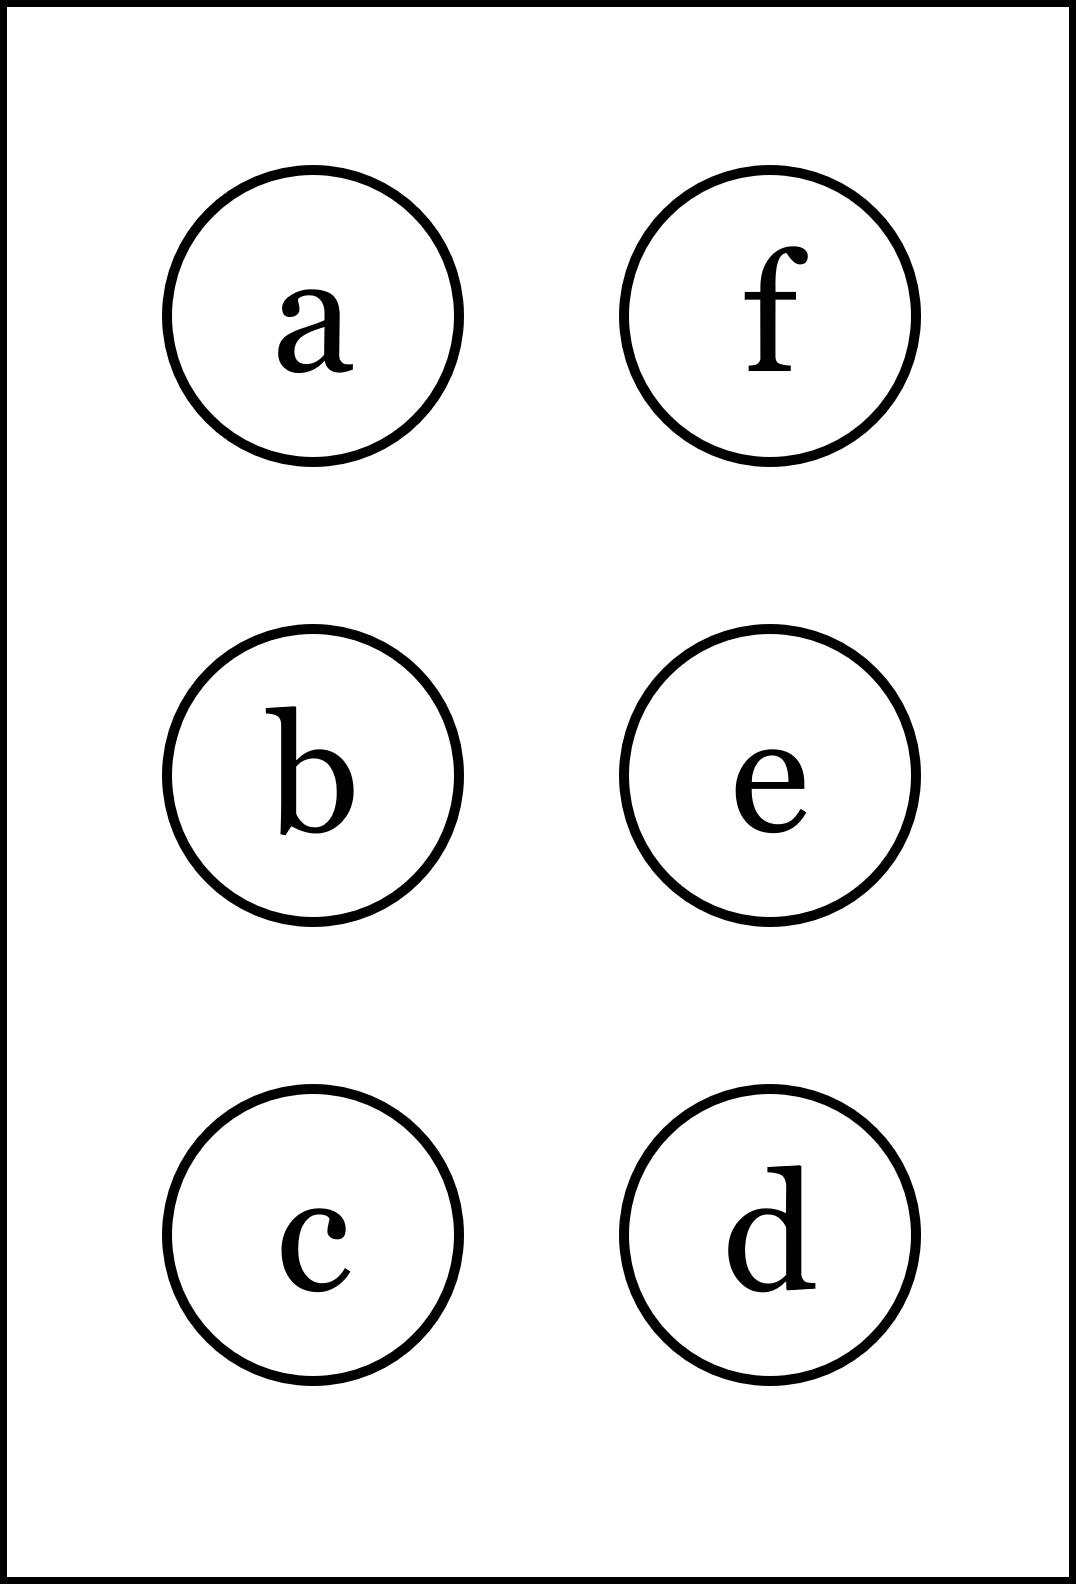
\includegraphics[height=40mm]{../images/braille.png}
{\small Písmeno Braillovej abecedy}
\end{center}
\end{minipage}
\end{center}
\end{minipage}
\\ \hdashline
\begin{minipage}[c][104.5mm][t]{0.5\linewidth}
\begin{center}
\vspace{7mm}
{\huge Tečna funkce, skupina \textit{Kappa $\kappa$} -\romannumeral3}\\[5mm]
\textit{Meno:}\phantom{xxxxxxxxxxxxxxxxxxxxxxxxxxxxxxxxxxxxxxxxxxxxxxxxxxxxxxxxxxxxxxxxx}\\[5mm]
\begin{minipage}{0.95\linewidth}
\begin{center}
V \textbf{(a)} a \textbf{(b)} urči \text{rovnicu tečny} $y = kx + q$ ku funkci $f(x)$ v bode $x_0$.\\V \textbf{(c)} a \textbf{(d)} urči ypsilonové souřadnice bodů, ve kterých je sklon $f(x)$ rovný $k$.\\Pokud se výsledky shodujú s těmi za otazníky, tak napravo obarvi\\příslušející kroužek načerno. \textbf{Spolu odevzdejte výsledné slovo}.
\end{center}
\end{minipage}
\\[1mm]
\begin{minipage}{0.79\linewidth}
\begin{center}
\begin{varwidth}{\linewidth}
\begin{enumerate}
\small
\item $f(x)=\cfrac{-3x+4}{-3x+7}\enspace , \enspace x_0=-3$\quad \dotfill\; ???\;\dotfill \quad $y = -\frac{9}{256}x+\frac{181}{256}$
\item $f(x)=-4\sqrt{-3x-1}\enspace , \enspace x_0=-\frac{2}{3}$\quad \dotfill\; ???\;\dotfill \quad $y = 6x+0$
\item $f(x)=-3x^2-x-1\enspace , \enspace k=-9$\quad \dotfill\; ???\;\dotfill \quad $-\frac{23}{3}$
\item $f(x)=x^3-3x^2-11x+4\enspace , \enspace k=-2$\quad \dotfill\; ???\;\dotfill \quad $11 , 37$
\item \quad \dotfill\; ???\;\dotfill \quad nebarvi
\item \quad \dotfill\; ???\;\dotfill \quad vybarvi
\end{enumerate}
\end{varwidth}
\end{center}
\end{minipage}
\begin{minipage}{0.20\linewidth}
\begin{center}
{\Huge\bfseries 3.} \\[2mm]
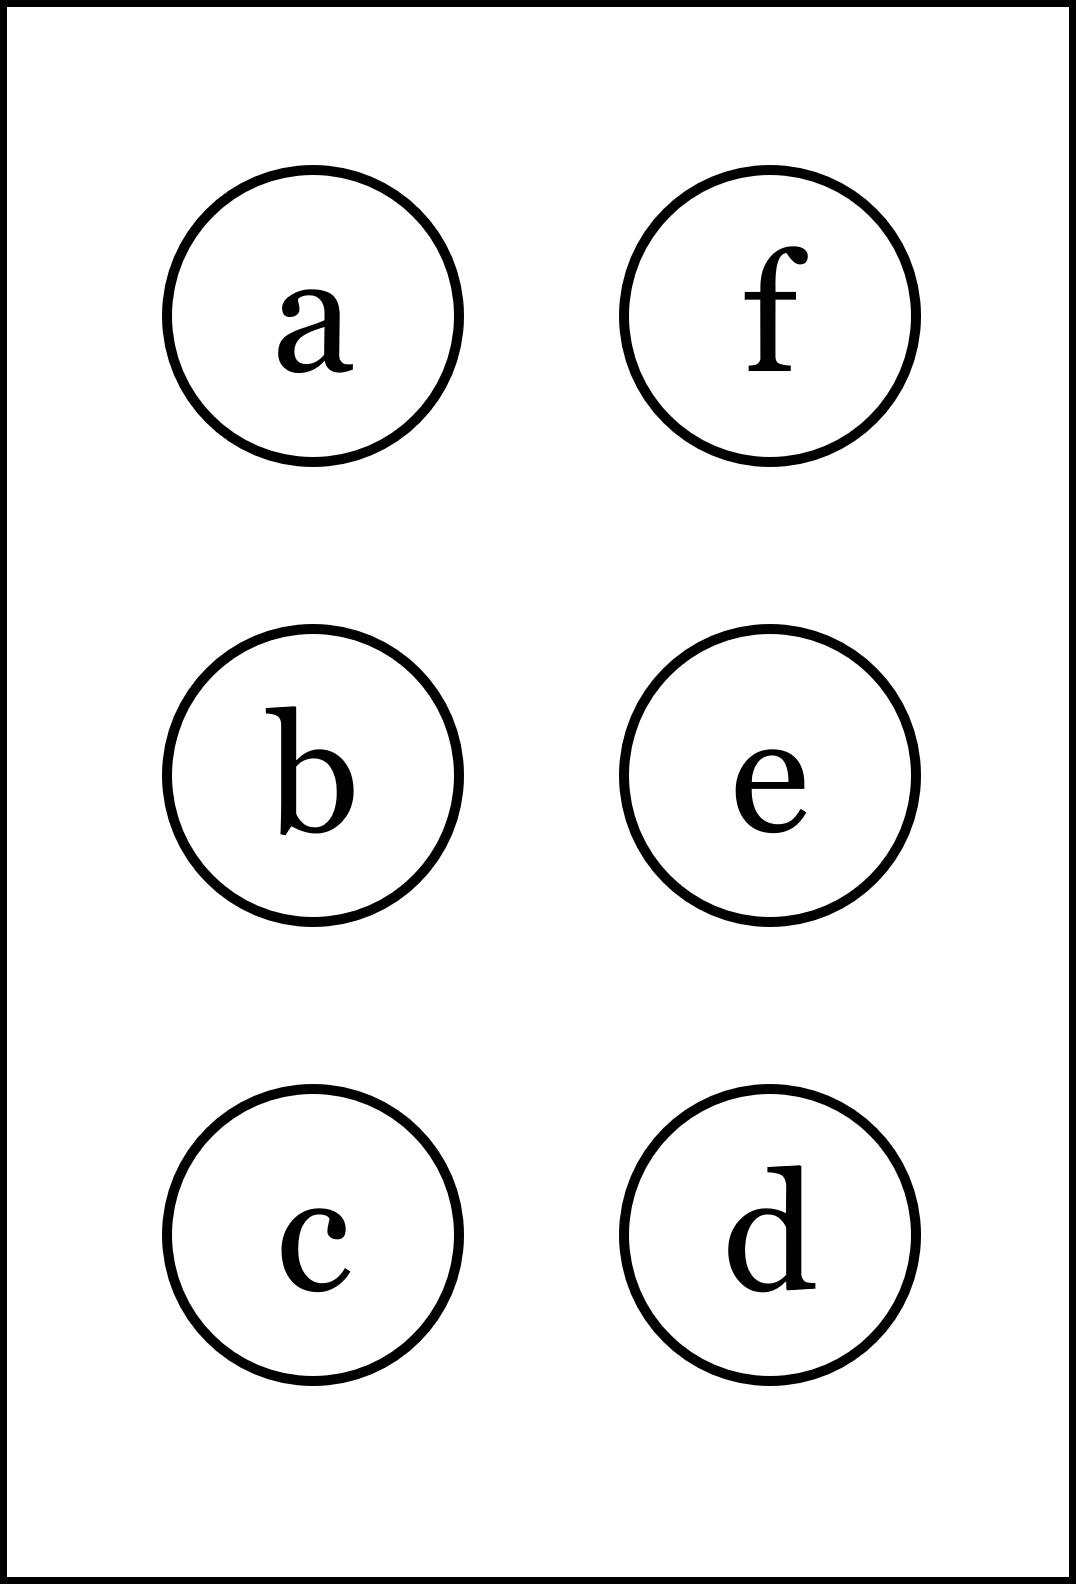
\includegraphics[height=40mm]{../images/braille.png}
{\small Písmeno Braillovej abecedy}
\end{center}
\end{minipage}
\end{center}
\end{minipage}
&
\begin{minipage}[c][104.5mm][t]{0.5\linewidth}
\begin{center}
\vspace{7mm}
{\huge Tečna funkce, skupina \textit{Kappa $\kappa$} -\romannumeral4}\\[5mm]
\textit{Meno:}\phantom{xxxxxxxxxxxxxxxxxxxxxxxxxxxxxxxxxxxxxxxxxxxxxxxxxxxxxxxxxxxxxxxxx}\\[5mm]
\begin{minipage}{0.95\linewidth}
\begin{center}
V \textbf{(a)} a \textbf{(b)} urči \text{rovnicu tečny} $y = kx + q$ ku funkci $f(x)$ v bode $x_0$.\\V \textbf{(c)} a \textbf{(d)} urči ypsilonové souřadnice bodů, ve kterých je sklon $f(x)$ rovný $k$.\\Pokud se výsledky shodujú s těmi za otazníky, tak napravo obarvi\\příslušející kroužek načerno. \textbf{Spolu odevzdejte výsledné slovo}.
\end{center}
\end{minipage}
\\[1mm]
\begin{minipage}{0.79\linewidth}
\begin{center}
\begin{varwidth}{\linewidth}
\begin{enumerate}
\small
\item $f(x)=\cfrac{-2x+6}{-2x-4}\enspace , \enspace x_0=2$\quad \dotfill\; ???\;\dotfill \quad $y = \frac{5}{16}x-\frac{7}{8}$
\item $f(x)=-6\sqrt{-5x+1}\enspace , \enspace x_0=-\frac{3}{5}$\quad \dotfill\; ???\;\dotfill \quad $y = \frac{15}{2}x-15$
\item $f(x)=-5x^2-7x+1\enspace , \enspace k=-7$\quad \dotfill\; ???\;\dotfill \quad $1$
\item $f(x)=2x^3-12x^2-28x+2\enspace , \enspace k=2$\quad \dotfill\; ???\;\dotfill \quad $16 , -188$
\item \quad \dotfill\; ???\;\dotfill \quad vybarvi
\item \quad \dotfill\; ???\;\dotfill \quad vybarvi
\end{enumerate}
\end{varwidth}
\end{center}
\end{minipage}
\begin{minipage}{0.20\linewidth}
\begin{center}
{\Huge\bfseries 4.} \\[2mm]
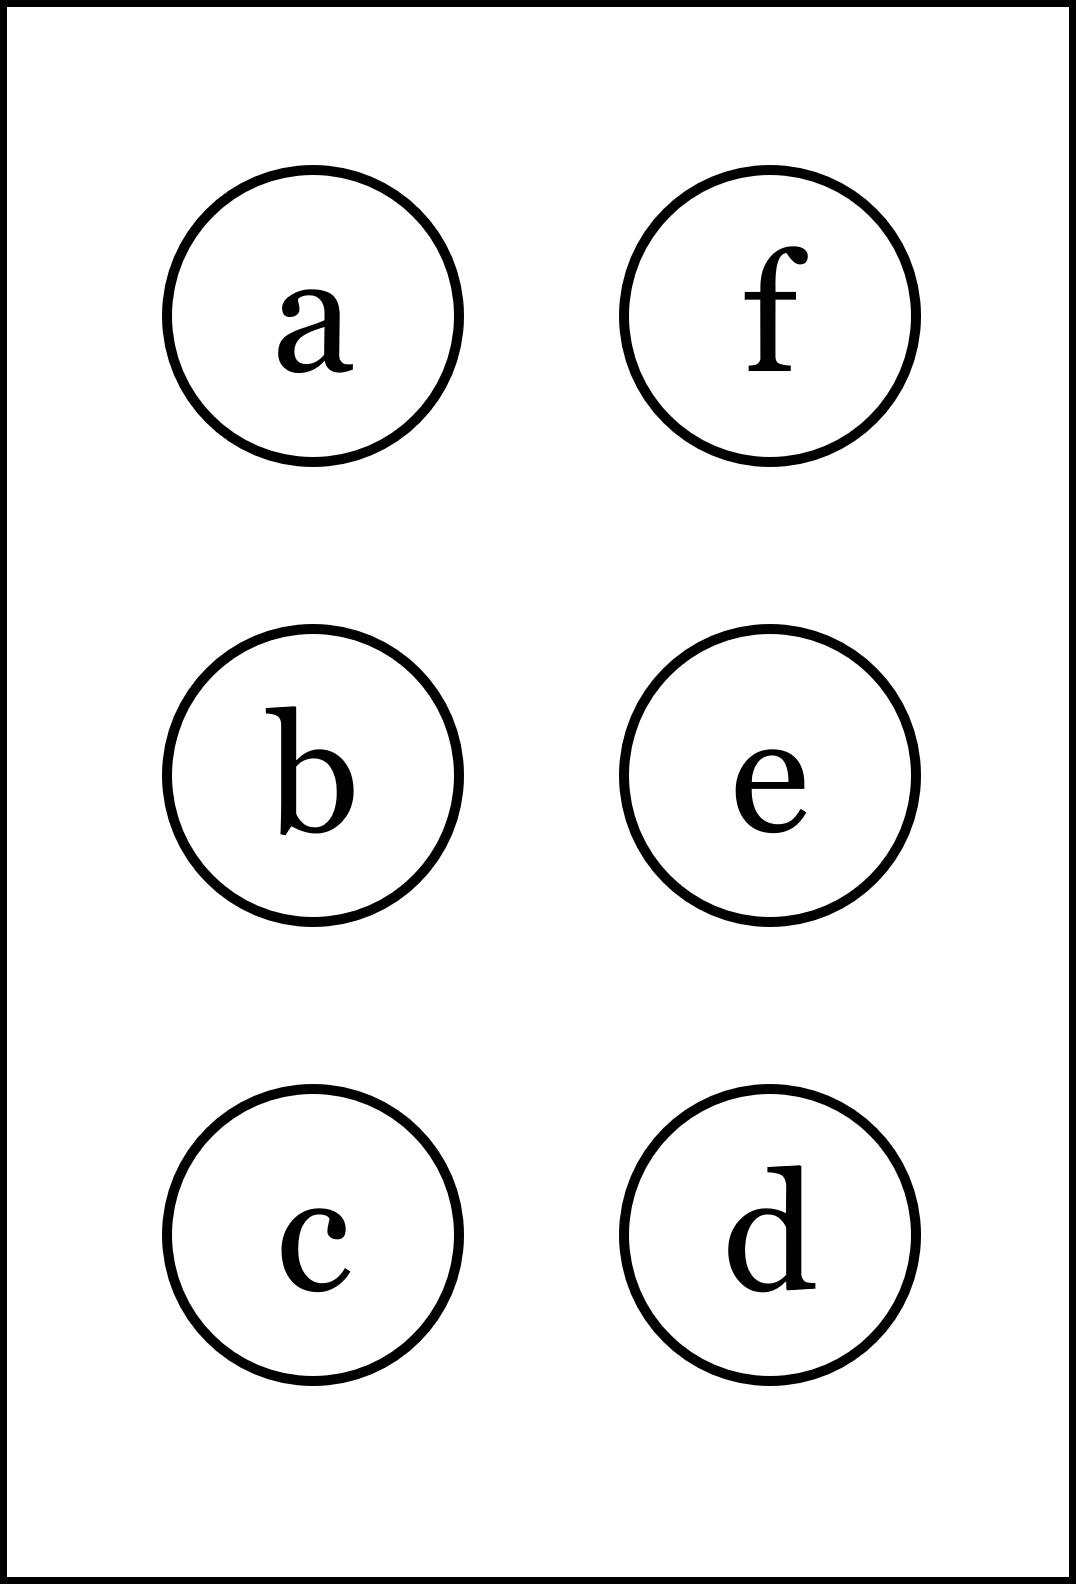
\includegraphics[height=40mm]{../images/braille.png}
{\small Písmeno Braillovej abecedy}
\end{center}
\end{minipage}
\end{center}
\end{minipage}
%
\end{tabular}
\newpage
\thispagestyle{empty}
\begin{tabular}{c:c}
\begin{minipage}[c][104.5mm][t]{0.5\linewidth}
\begin{center}
\vspace{7mm}
{\huge Tečna funkce, skupina \textit{Lambda $\lambda$} -\romannumeral1}\\[5mm]
\textit{Meno:}\phantom{xxxxxxxxxxxxxxxxxxxxxxxxxxxxxxxxxxxxxxxxxxxxxxxxxxxxxxxxxxxxxxxxx}\\[5mm]
\begin{minipage}{0.95\linewidth}
\begin{center}
V \textbf{(a)} a \textbf{(b)} urči \text{rovnicu tečny} $y = kx + q$ ku funkci $f(x)$ v bode $x_0$.\\V \textbf{(c)} a \textbf{(d)} urči ypsilonové souřadnice bodů, ve kterých je sklon $f(x)$ rovný $k$.\\Pokud se výsledky shodujú s těmi za otazníky, tak napravo obarvi\\příslušející kroužek načerno. \textbf{Spolu odevzdejte výsledné slovo}.
\end{center}
\end{minipage}
\\[1mm]
\begin{minipage}{0.79\linewidth}
\begin{center}
\begin{varwidth}{\linewidth}
\begin{enumerate}
\small
\item $f(x)=\cfrac{-8x+2}{x-3}\enspace , \enspace x_0=-3$\quad \dotfill\; ???\;\dotfill \quad $y = \frac{11}{18}x-\frac{5}{2}$
\item $f(x)=-3\sqrt{2x+1}\enspace , \enspace x_0=0$\quad \dotfill\; ???\;\dotfill \quad $y = -3x-6$
\item $f(x)=-9x^2-2x-4\enspace , \enspace k=1$\quad \dotfill\; ???\;\dotfill \quad $-\frac{47}{12}$
\item $f(x)=3x^3-9x^2-30x+5\enspace , \enspace k=-3$\quad \dotfill\; ???\;\dotfill \quad $23 , -85$
\item \quad \dotfill\; ???\;\dotfill \quad vybarvi
\item \quad \dotfill\; ???\;\dotfill \quad nebarvi
\end{enumerate}
\end{varwidth}
\end{center}
\end{minipage}
\begin{minipage}{0.20\linewidth}
\begin{center}
{\Huge\bfseries 1.} \\[2mm]
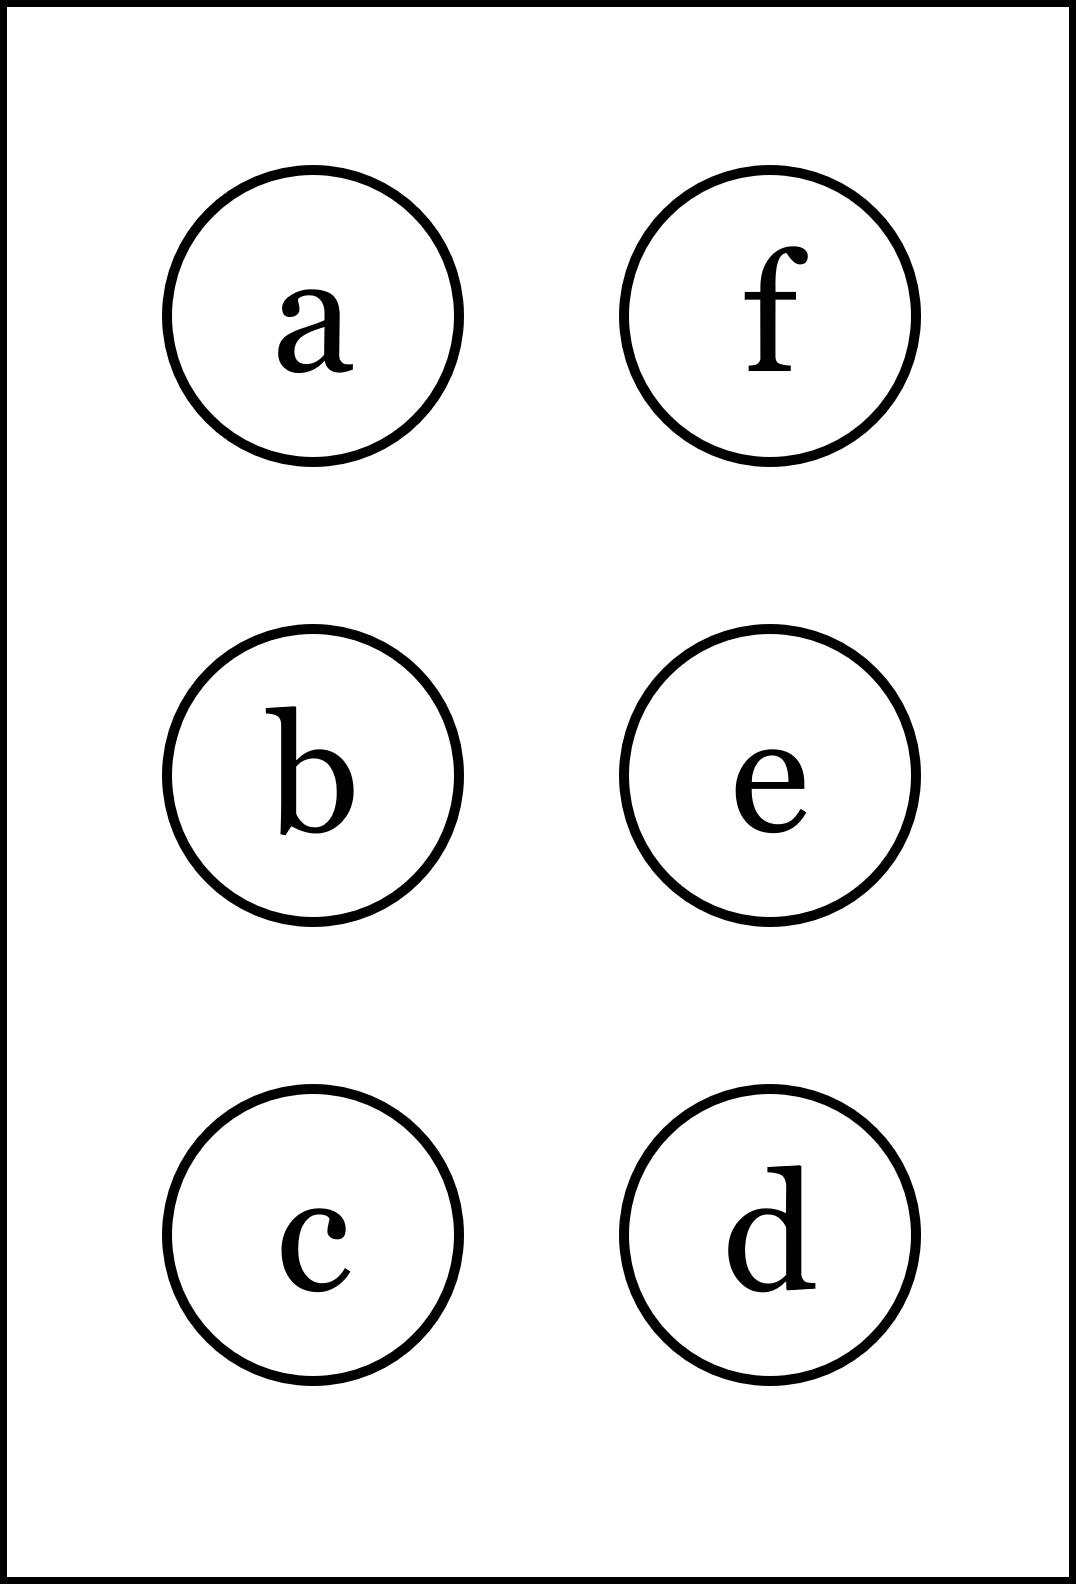
\includegraphics[height=40mm]{../images/braille.png}
{\small Písmeno Braillovej abecedy}
\end{center}
\end{minipage}
\end{center}
\end{minipage}
&
\begin{minipage}[c][104.5mm][t]{0.5\linewidth}
\begin{center}
\vspace{7mm}
{\huge Tečna funkce, skupina \textit{Lambda $\lambda$} -\romannumeral2}\\[5mm]
\textit{Meno:}\phantom{xxxxxxxxxxxxxxxxxxxxxxxxxxxxxxxxxxxxxxxxxxxxxxxxxxxxxxxxxxxxxxxxx}\\[5mm]
\begin{minipage}{0.95\linewidth}
\begin{center}
V \textbf{(a)} a \textbf{(b)} urči \text{rovnicu tečny} $y = kx + q$ ku funkci $f(x)$ v bode $x_0$.\\V \textbf{(c)} a \textbf{(d)} urči ypsilonové souřadnice bodů, ve kterých je sklon $f(x)$ rovný $k$.\\Pokud se výsledky shodujú s těmi za otazníky, tak napravo obarvi\\příslušející kroužek načerno. \textbf{Spolu odevzdejte výsledné slovo}.
\end{center}
\end{minipage}
\\[1mm]
\begin{minipage}{0.79\linewidth}
\begin{center}
\begin{varwidth}{\linewidth}
\begin{enumerate}
\small
\item $f(x)=\cfrac{4x-6}{x-4}\enspace , \enspace x_0=-2$\quad \dotfill\; ???\;\dotfill \quad $y = -\frac{5}{18}x+\frac{16}{9}$
\item $f(x)=5\sqrt{-4x+2}\enspace , \enspace x_0=-\frac{23}{4}$\quad \dotfill\; ???\;\dotfill \quad $y = -2x+27$
\item $f(x)=3x^2-2x-2\enspace , \enspace k=2$\quad \dotfill\; ???\;\dotfill \quad $-2$
\item $f(x)=5x^3-30x^2-179x+5\enspace , \enspace k=1$\quad \dotfill\; ???\;\dotfill \quad $203 , -1069$
\item \quad \dotfill\; ???\;\dotfill \quad nebarvi
\item \quad \dotfill\; ???\;\dotfill \quad nebarvi
\end{enumerate}
\end{varwidth}
\end{center}
\end{minipage}
\begin{minipage}{0.20\linewidth}
\begin{center}
{\Huge\bfseries 2.} \\[2mm]
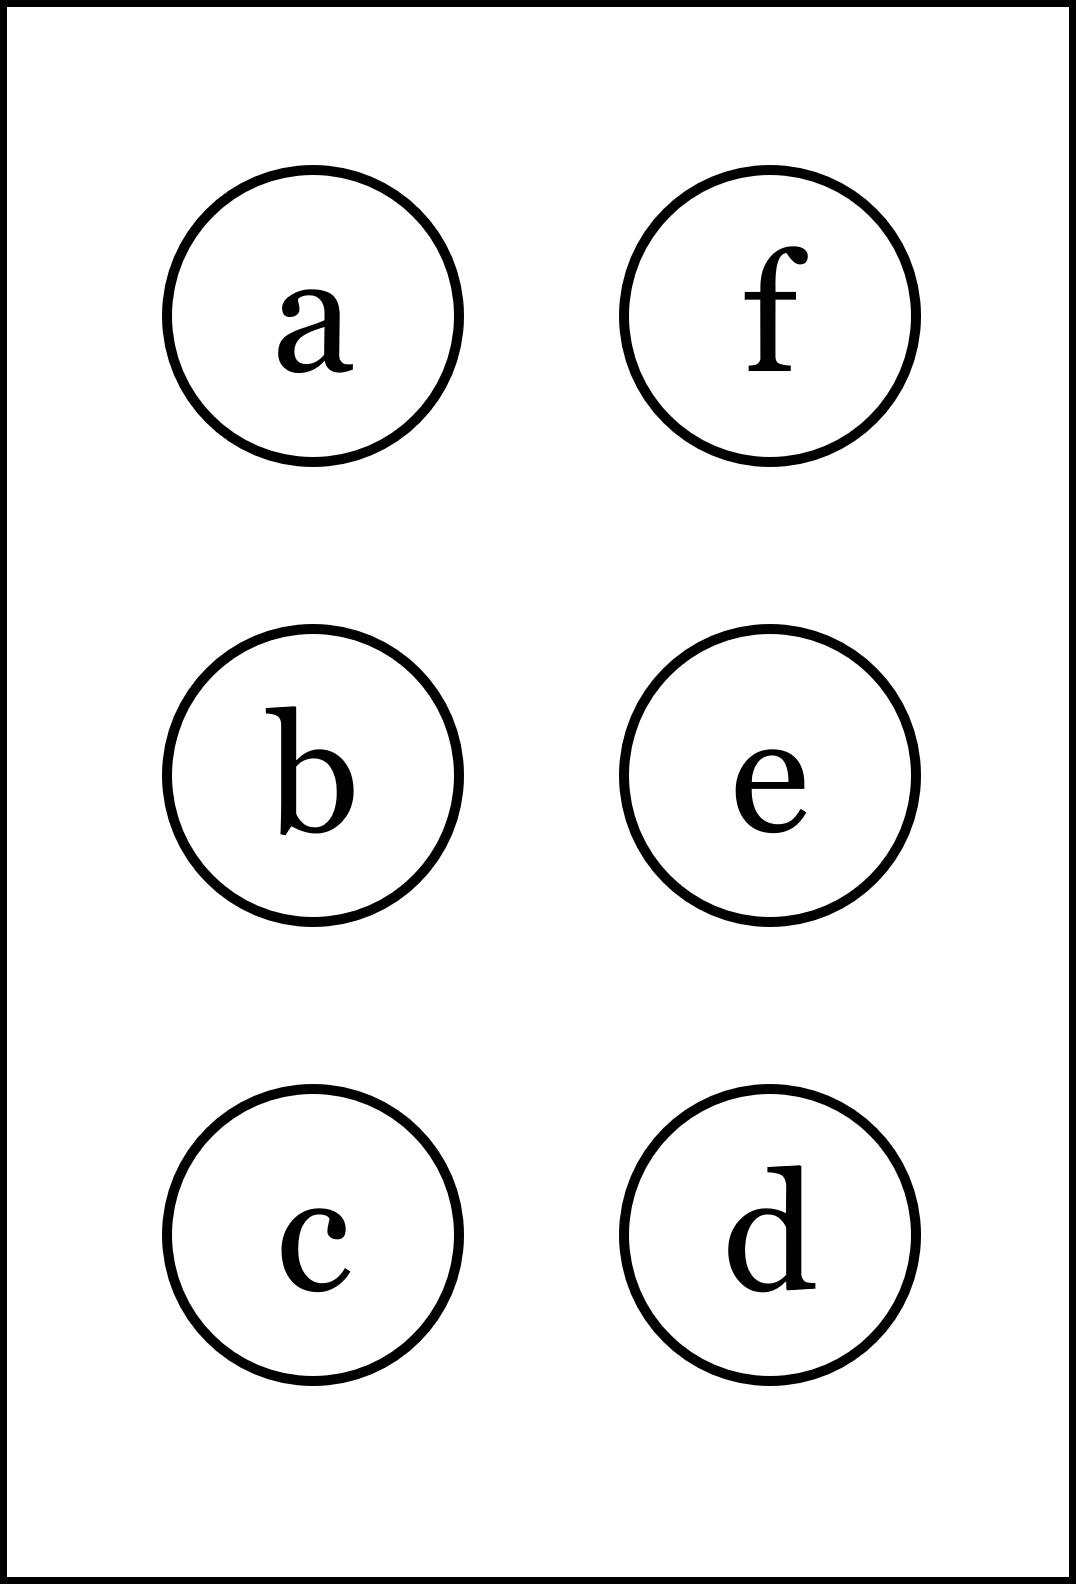
\includegraphics[height=40mm]{../images/braille.png}
{\small Písmeno Braillovej abecedy}
\end{center}
\end{minipage}
\end{center}
\end{minipage}
\\ \hdashline
\begin{minipage}[c][104.5mm][t]{0.5\linewidth}
\begin{center}
\vspace{7mm}
{\huge Tečna funkce, skupina \textit{Lambda $\lambda$} -\romannumeral3}\\[5mm]
\textit{Meno:}\phantom{xxxxxxxxxxxxxxxxxxxxxxxxxxxxxxxxxxxxxxxxxxxxxxxxxxxxxxxxxxxxxxxxx}\\[5mm]
\begin{minipage}{0.95\linewidth}
\begin{center}
V \textbf{(a)} a \textbf{(b)} urči \text{rovnicu tečny} $y = kx + q$ ku funkci $f(x)$ v bode $x_0$.\\V \textbf{(c)} a \textbf{(d)} urči ypsilonové souřadnice bodů, ve kterých je sklon $f(x)$ rovný $k$.\\Pokud se výsledky shodujú s těmi za otazníky, tak napravo obarvi\\příslušející kroužek načerno. \textbf{Spolu odevzdejte výsledné slovo}.
\end{center}
\end{minipage}
\\[1mm]
\begin{minipage}{0.79\linewidth}
\begin{center}
\begin{varwidth}{\linewidth}
\begin{enumerate}
\small
\item $f(x)=\cfrac{-x-1}{-6x-6}\enspace , \enspace x_0=1$\quad \dotfill\; ???\;\dotfill \quad $y = 0x+\frac{1}{6}$
\item $f(x)=-4\sqrt{-x+8}\enspace , \enspace x_0=4$\quad \dotfill\; ???\;\dotfill \quad $y = x-12$
\item $f(x)=-3x^2-2x+4\enspace , \enspace k=9$\quad \dotfill\; ???\;\dotfill \quad $-\frac{125}{12}$
\item $f(x)=2x^3-12x^2+14x-1\enspace , \enspace k=-4$\quad \dotfill\; ???\;\dotfill \quad $3 , -97$
\item \quad \dotfill\; ???\;\dotfill \quad nebarvi
\item \quad \dotfill\; ???\;\dotfill \quad nebarvi
\end{enumerate}
\end{varwidth}
\end{center}
\end{minipage}
\begin{minipage}{0.20\linewidth}
\begin{center}
{\Huge\bfseries 3.} \\[2mm]
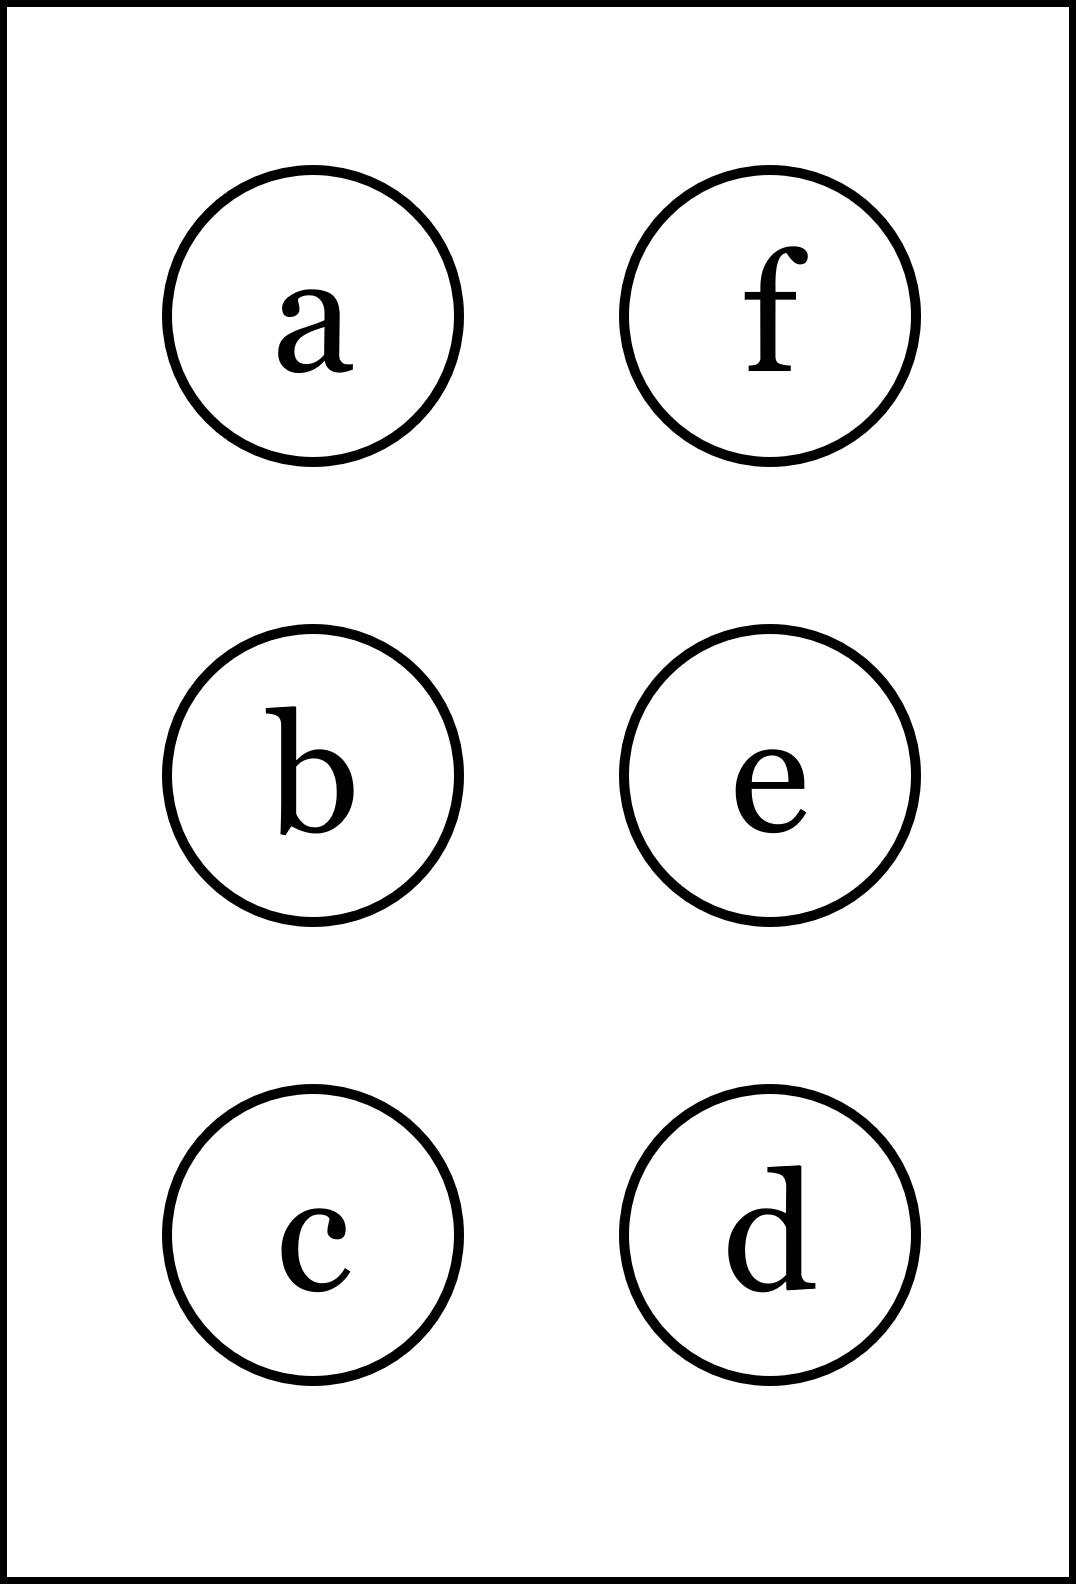
\includegraphics[height=40mm]{../images/braille.png}
{\small Písmeno Braillovej abecedy}
\end{center}
\end{minipage}
\end{center}
\end{minipage}
&
\begin{minipage}[c][104.5mm][t]{0.5\linewidth}
\begin{center}
\vspace{7mm}
{\huge Tečna funkce, skupina \textit{Lambda $\lambda$} -\romannumeral4}\\[5mm]
\textit{Meno:}\phantom{xxxxxxxxxxxxxxxxxxxxxxxxxxxxxxxxxxxxxxxxxxxxxxxxxxxxxxxxxxxxxxxxx}\\[5mm]
\begin{minipage}{0.95\linewidth}
\begin{center}
V \textbf{(a)} a \textbf{(b)} urči \text{rovnicu tečny} $y = kx + q$ ku funkci $f(x)$ v bode $x_0$.\\V \textbf{(c)} a \textbf{(d)} urči ypsilonové souřadnice bodů, ve kterých je sklon $f(x)$ rovný $k$.\\Pokud se výsledky shodujú s těmi za otazníky, tak napravo obarvi\\příslušející kroužek načerno. \textbf{Spolu odevzdejte výsledné slovo}.
\end{center}
\end{minipage}
\\[1mm]
\begin{minipage}{0.79\linewidth}
\begin{center}
\begin{varwidth}{\linewidth}
\begin{enumerate}
\small
\item $f(x)=\cfrac{-4x+7}{-4x+1}\enspace , \enspace x_0=1$\quad \dotfill\; ???\;\dotfill \quad $y = \frac{8}{3}x-\frac{11}{3}$
\item $f(x)=8\sqrt{x-1}\enspace , \enspace x_0=26$\quad \dotfill\; ???\;\dotfill \quad $y = \frac{4}{5}x+\frac{192}{5}$
\item $f(x)=5x^2+x-1\enspace , \enspace k=-5$\quad \dotfill\; ???\;\dotfill \quad $\frac{1}{5}$
\item $f(x)=4x^3-12x^2-39x+3\enspace , \enspace k=-3$\quad \dotfill\; ???\;\dotfill \quad $26 , -114$
\item \quad \dotfill\; ???\;\dotfill \quad vybarvi
\item \quad \dotfill\; ???\;\dotfill \quad vybarvi
\end{enumerate}
\end{varwidth}
\end{center}
\end{minipage}
\begin{minipage}{0.20\linewidth}
\begin{center}
{\Huge\bfseries 4.} \\[2mm]
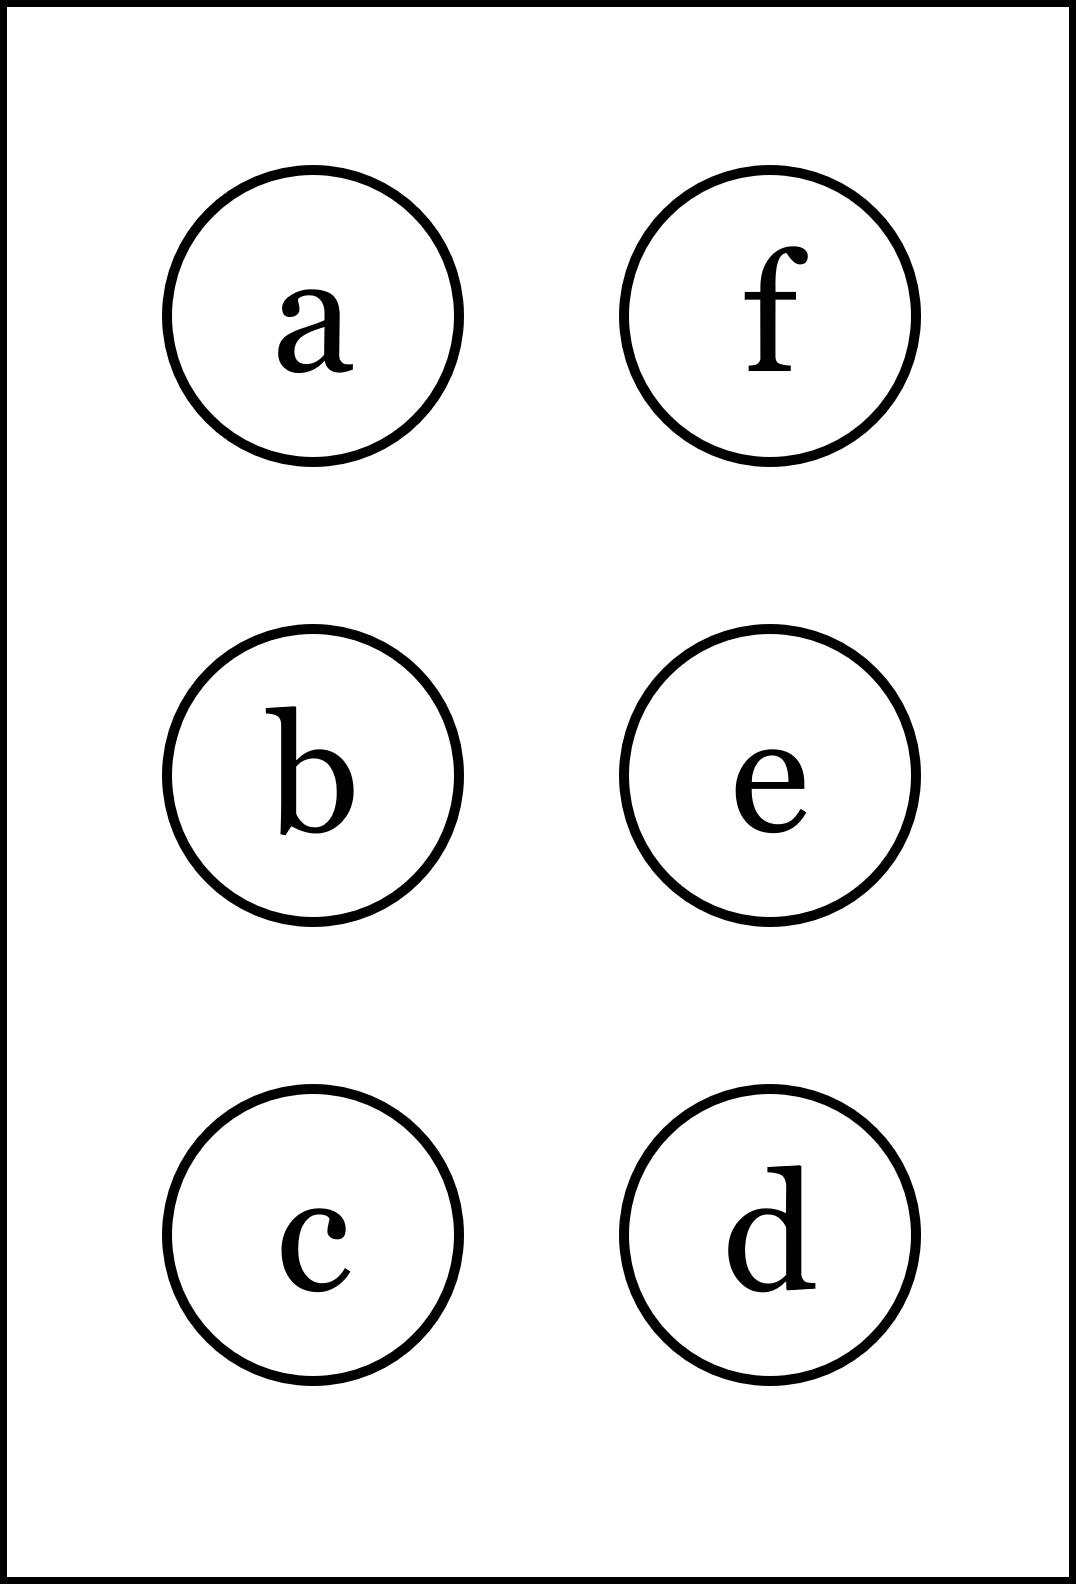
\includegraphics[height=40mm]{../images/braille.png}
{\small Písmeno Braillovej abecedy}
\end{center}
\end{minipage}
\end{center}
\end{minipage}
%
\end{tabular}
\newpage
\thispagestyle{empty}
\begin{tabular}{c:c}
\begin{minipage}[c][104.5mm][t]{0.5\linewidth}
\begin{center}
\vspace{7mm}
{\huge Tečna funkce, skupina \textit{Mu $\mu$} -\romannumeral1}\\[5mm]
\textit{Meno:}\phantom{xxxxxxxxxxxxxxxxxxxxxxxxxxxxxxxxxxxxxxxxxxxxxxxxxxxxxxxxxxxxxxxxx}\\[5mm]
\begin{minipage}{0.95\linewidth}
\begin{center}
V \textbf{(a)} a \textbf{(b)} urči \text{rovnicu tečny} $y = kx + q$ ku funkci $f(x)$ v bode $x_0$.\\V \textbf{(c)} a \textbf{(d)} urči ypsilonové souřadnice bodů, ve kterých je sklon $f(x)$ rovný $k$.\\Pokud se výsledky shodujú s těmi za otazníky, tak napravo obarvi\\příslušející kroužek načerno. \textbf{Spolu odevzdejte výsledné slovo}.
\end{center}
\end{minipage}
\\[1mm]
\begin{minipage}{0.79\linewidth}
\begin{center}
\begin{varwidth}{\linewidth}
\begin{enumerate}
\small
\item $f(x)=\cfrac{2x-4}{-3x-3}\enspace , \enspace x_0=-2$\quad \dotfill\; ???\;\dotfill \quad $y = -2x-\frac{20}{3}$
\item $f(x)=-2\sqrt{5x-1}\enspace , \enspace x_0=1$\quad \dotfill\; ???\;\dotfill \quad $y = -\frac{5}{2}x-\frac{3}{2}$
\item $f(x)=-3x^2-5x+4\enspace , \enspace k=4$\quad \dotfill\; ???\;\dotfill \quad $\frac{19}{4}$
\item $f(x)=3x^3-9x^2-71x+4\enspace , \enspace k=1$\quad \dotfill\; ???\;\dotfill \quad $86 , -232$
\item \quad \dotfill\; ???\;\dotfill \quad vybarvi
\item \quad \dotfill\; ???\;\dotfill \quad nebarvi
\end{enumerate}
\end{varwidth}
\end{center}
\end{minipage}
\begin{minipage}{0.20\linewidth}
\begin{center}
{\Huge\bfseries 1.} \\[2mm]
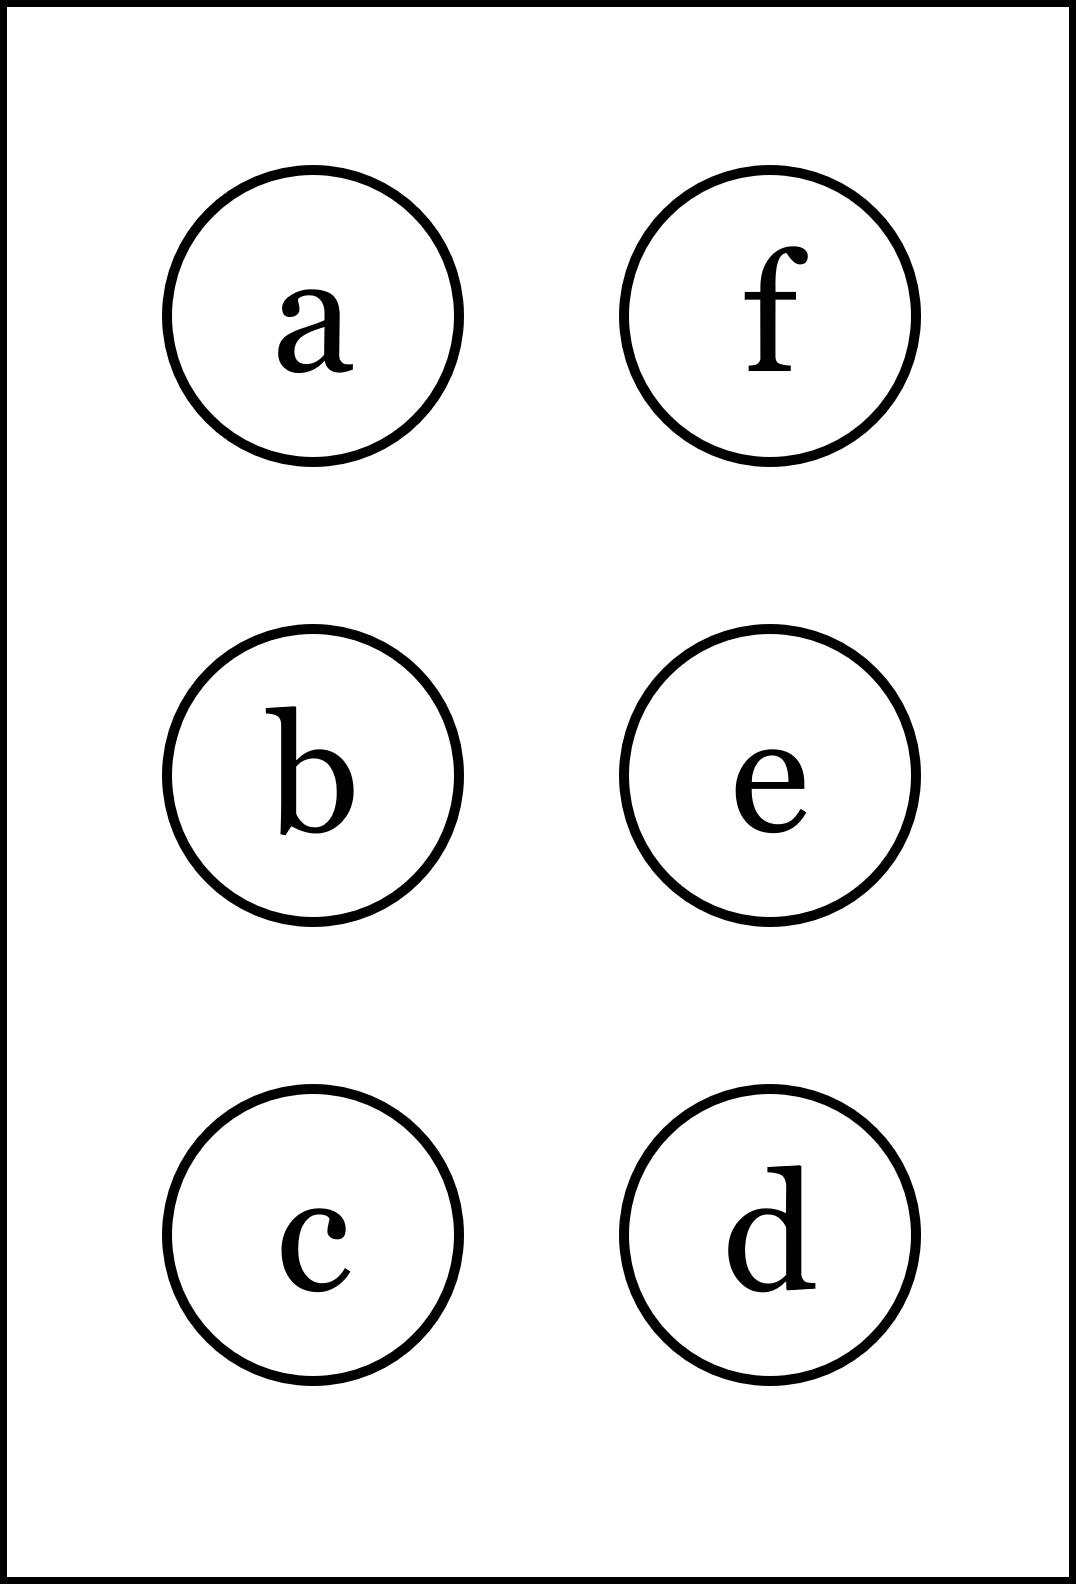
\includegraphics[height=40mm]{../images/braille.png}
{\small Písmeno Braillovej abecedy}
\end{center}
\end{minipage}
\end{center}
\end{minipage}
&
\begin{minipage}[c][104.5mm][t]{0.5\linewidth}
\begin{center}
\vspace{7mm}
{\huge Tečna funkce, skupina \textit{Mu $\mu$} -\romannumeral2}\\[5mm]
\textit{Meno:}\phantom{xxxxxxxxxxxxxxxxxxxxxxxxxxxxxxxxxxxxxxxxxxxxxxxxxxxxxxxxxxxxxxxxx}\\[5mm]
\begin{minipage}{0.95\linewidth}
\begin{center}
V \textbf{(a)} a \textbf{(b)} urči \text{rovnicu tečny} $y = kx + q$ ku funkci $f(x)$ v bode $x_0$.\\V \textbf{(c)} a \textbf{(d)} urči ypsilonové souřadnice bodů, ve kterých je sklon $f(x)$ rovný $k$.\\Pokud se výsledky shodujú s těmi za otazníky, tak napravo obarvi\\příslušející kroužek načerno. \textbf{Spolu odevzdejte výsledné slovo}.
\end{center}
\end{minipage}
\\[1mm]
\begin{minipage}{0.79\linewidth}
\begin{center}
\begin{varwidth}{\linewidth}
\begin{enumerate}
\small
\item $f(x)=\cfrac{5x+3}{-2x-3}\enspace , \enspace x_0=-3$\quad \dotfill\; ???\;\dotfill \quad $y = -x-15$
\item $f(x)=\sqrt{5x+5}\enspace , \enspace x_0=-\frac{1}{5}$\quad \dotfill\; ???\;\dotfill \quad $y = \frac{5}{4}x+\frac{9}{4}$
\item $f(x)=-3x^2-5x-5\enspace , \enspace k=-5$\quad \dotfill\; ???\;\dotfill \quad $5$
\item $f(x)=3x^3-18x^2-105x+3\enspace , \enspace k=3$\quad \dotfill\; ???\;\dotfill \quad $117 , 633$
\item \quad \dotfill\; ???\;\dotfill \quad nebarvi
\item \quad \dotfill\; ???\;\dotfill \quad vybarvi
\end{enumerate}
\end{varwidth}
\end{center}
\end{minipage}
\begin{minipage}{0.20\linewidth}
\begin{center}
{\Huge\bfseries 2.} \\[2mm]
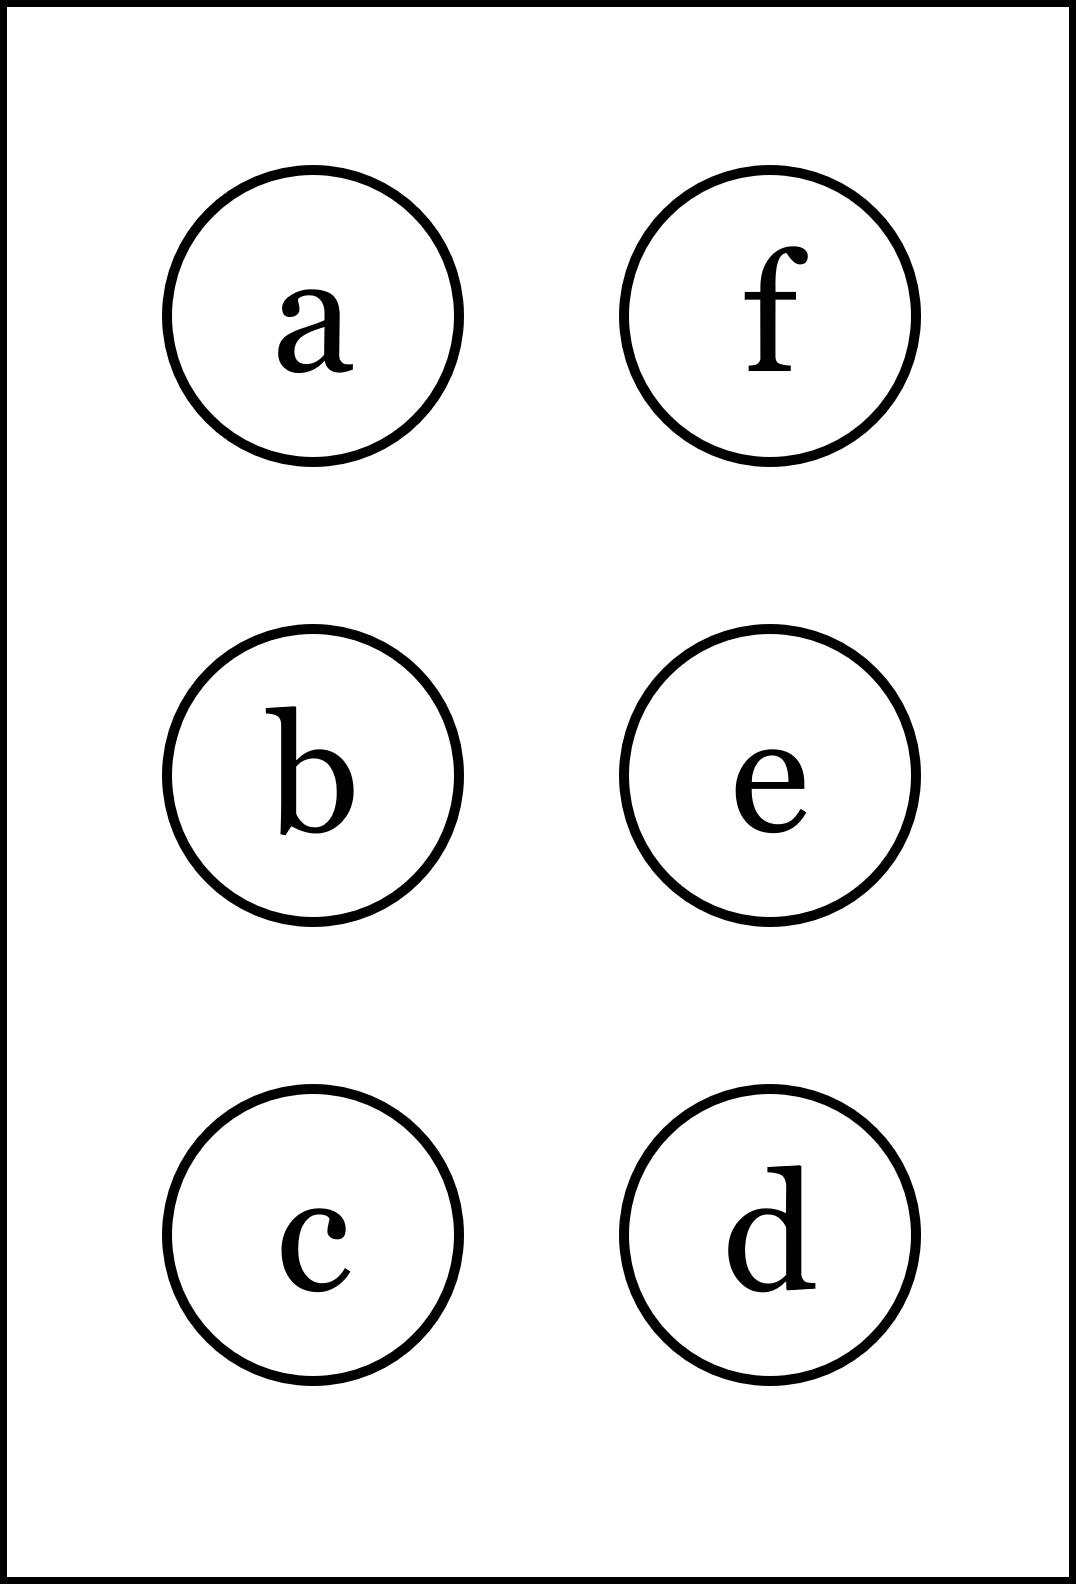
\includegraphics[height=40mm]{../images/braille.png}
{\small Písmeno Braillovej abecedy}
\end{center}
\end{minipage}
\end{center}
\end{minipage}
\\ \hdashline
\begin{minipage}[c][104.5mm][t]{0.5\linewidth}
\begin{center}
\vspace{7mm}
{\huge Tečna funkce, skupina \textit{Mu $\mu$} -\romannumeral3}\\[5mm]
\textit{Meno:}\phantom{xxxxxxxxxxxxxxxxxxxxxxxxxxxxxxxxxxxxxxxxxxxxxxxxxxxxxxxxxxxxxxxxx}\\[5mm]
\begin{minipage}{0.95\linewidth}
\begin{center}
V \textbf{(a)} a \textbf{(b)} urči \text{rovnicu tečny} $y = kx + q$ ku funkci $f(x)$ v bode $x_0$.\\V \textbf{(c)} a \textbf{(d)} urči ypsilonové souřadnice bodů, ve kterých je sklon $f(x)$ rovný $k$.\\Pokud se výsledky shodujú s těmi za otazníky, tak napravo obarvi\\příslušející kroužek načerno. \textbf{Spolu odevzdejte výsledné slovo}.
\end{center}
\end{minipage}
\\[1mm]
\begin{minipage}{0.79\linewidth}
\begin{center}
\begin{varwidth}{\linewidth}
\begin{enumerate}
\small
\item $f(x)=\cfrac{-3x+1}{-9x+8}\enspace , \enspace x_0=1$\quad \dotfill\; ???\;\dotfill \quad $y = -15x+17$
\item $f(x)=8\sqrt{4x-5}\enspace , \enspace x_0=\frac{9}{4}$\quad \dotfill\; ???\;\dotfill \quad $y = 8x-2$
\item $f(x)=x^2-4x+2\enspace , \enspace k=-4$\quad \dotfill\; ???\;\dotfill \quad $-2$
\item $f(x)=x^3+3x^2-8x+1\enspace , \enspace k=1$\quad \dotfill\; ???\;\dotfill \quad $25 , 13$
\item \quad \dotfill\; ???\;\dotfill \quad nebarvi
\item \quad \dotfill\; ???\;\dotfill \quad vybarvi
\end{enumerate}
\end{varwidth}
\end{center}
\end{minipage}
\begin{minipage}{0.20\linewidth}
\begin{center}
{\Huge\bfseries 3.} \\[2mm]
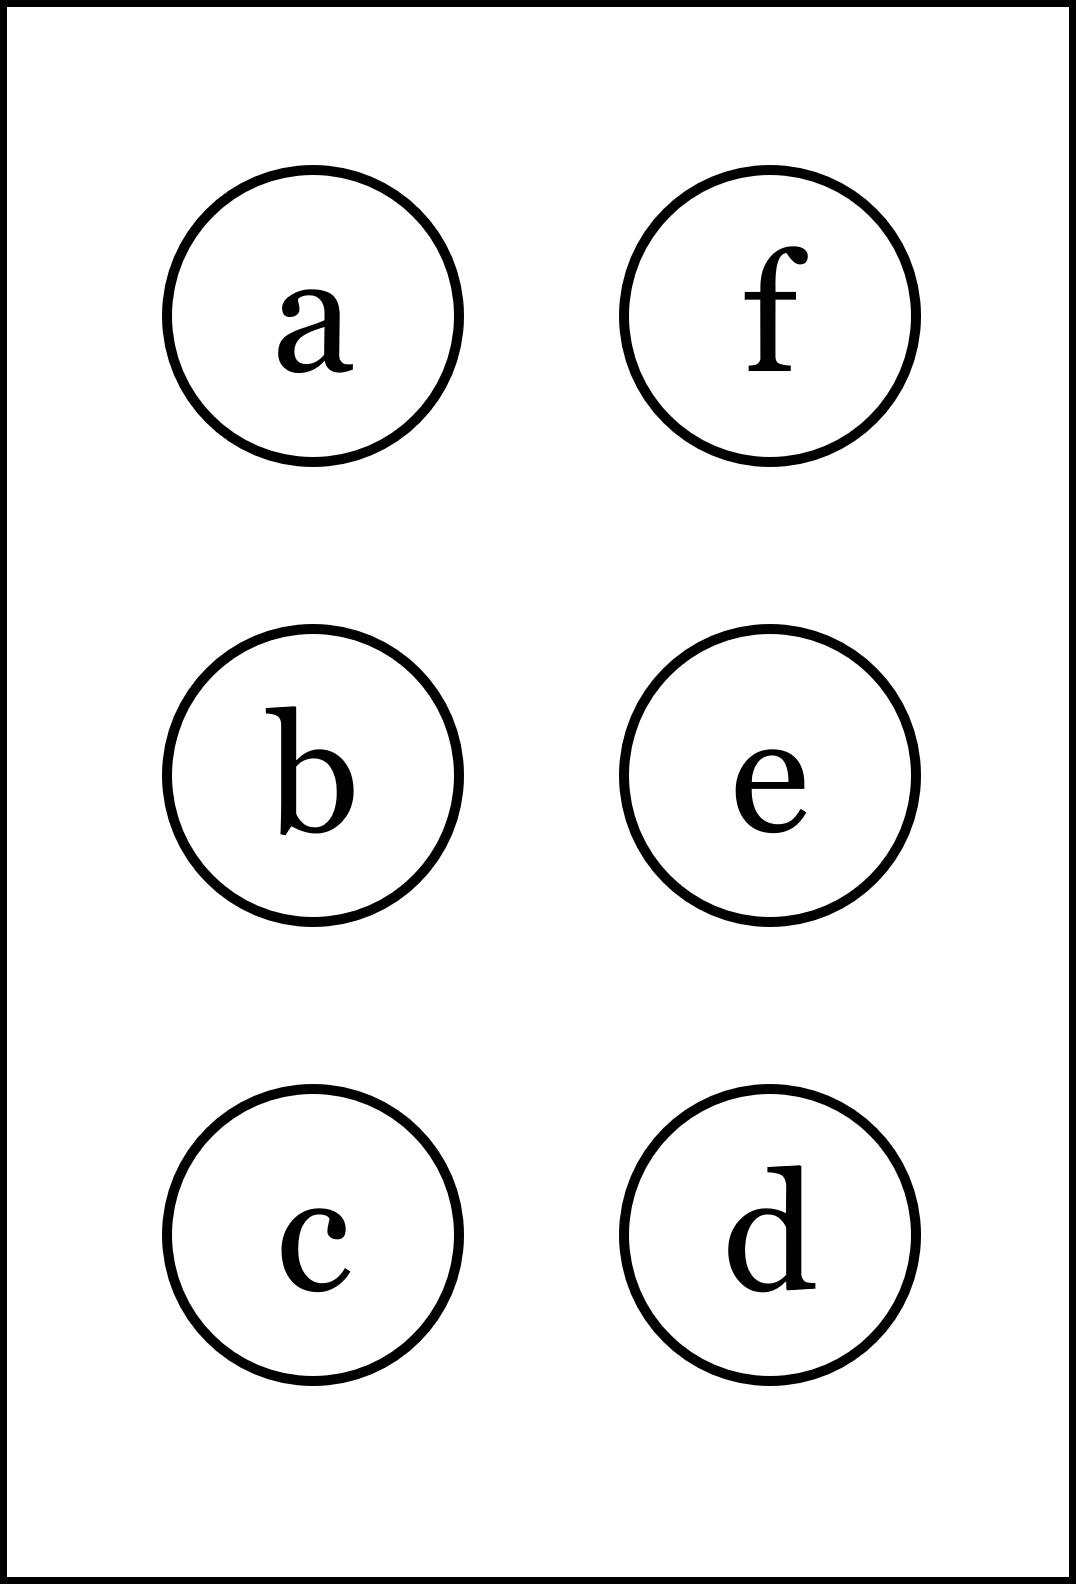
\includegraphics[height=40mm]{../images/braille.png}
{\small Písmeno Braillovej abecedy}
\end{center}
\end{minipage}
\end{center}
\end{minipage}
&
\begin{minipage}[c][104.5mm][t]{0.5\linewidth}
\begin{center}
\vspace{7mm}
{\huge Tečna funkce, skupina \textit{Mu $\mu$} -\romannumeral4}\\[5mm]
\textit{Meno:}\phantom{xxxxxxxxxxxxxxxxxxxxxxxxxxxxxxxxxxxxxxxxxxxxxxxxxxxxxxxxxxxxxxxxx}\\[5mm]
\begin{minipage}{0.95\linewidth}
\begin{center}
V \textbf{(a)} a \textbf{(b)} urči \text{rovnicu tečny} $y = kx + q$ ku funkci $f(x)$ v bode $x_0$.\\V \textbf{(c)} a \textbf{(d)} urči ypsilonové souřadnice bodů, ve kterých je sklon $f(x)$ rovný $k$.\\Pokud se výsledky shodujú s těmi za otazníky, tak napravo obarvi\\příslušející kroužek načerno. \textbf{Spolu odevzdejte výsledné slovo}.
\end{center}
\end{minipage}
\\[1mm]
\begin{minipage}{0.79\linewidth}
\begin{center}
\begin{varwidth}{\linewidth}
\begin{enumerate}
\small
\item $f(x)=\cfrac{x+5}{-2x-8}\enspace , \enspace x_0=2$\quad \dotfill\; ???\;\dotfill \quad $y = \frac{1}{72}x-\frac{1}{18}$
\item $f(x)=-6\sqrt{-2x+4}\enspace , \enspace x_0=0$\quad \dotfill\; ???\;\dotfill \quad $y = 3x-12$
\item $f(x)=x^2-6x+7\enspace , \enspace k=-2$\quad \dotfill\; ???\;\dotfill \quad $-15$
\item $f(x)=x^3-9x^2+16x+3\enspace , \enspace k=1$\quad \dotfill\; ???\;\dotfill \quad $11 , -177$
\item \quad \dotfill\; ???\;\dotfill \quad nebarvi
\item \quad \dotfill\; ???\;\dotfill \quad vybarvi
\end{enumerate}
\end{varwidth}
\end{center}
\end{minipage}
\begin{minipage}{0.20\linewidth}
\begin{center}
{\Huge\bfseries 4.} \\[2mm]
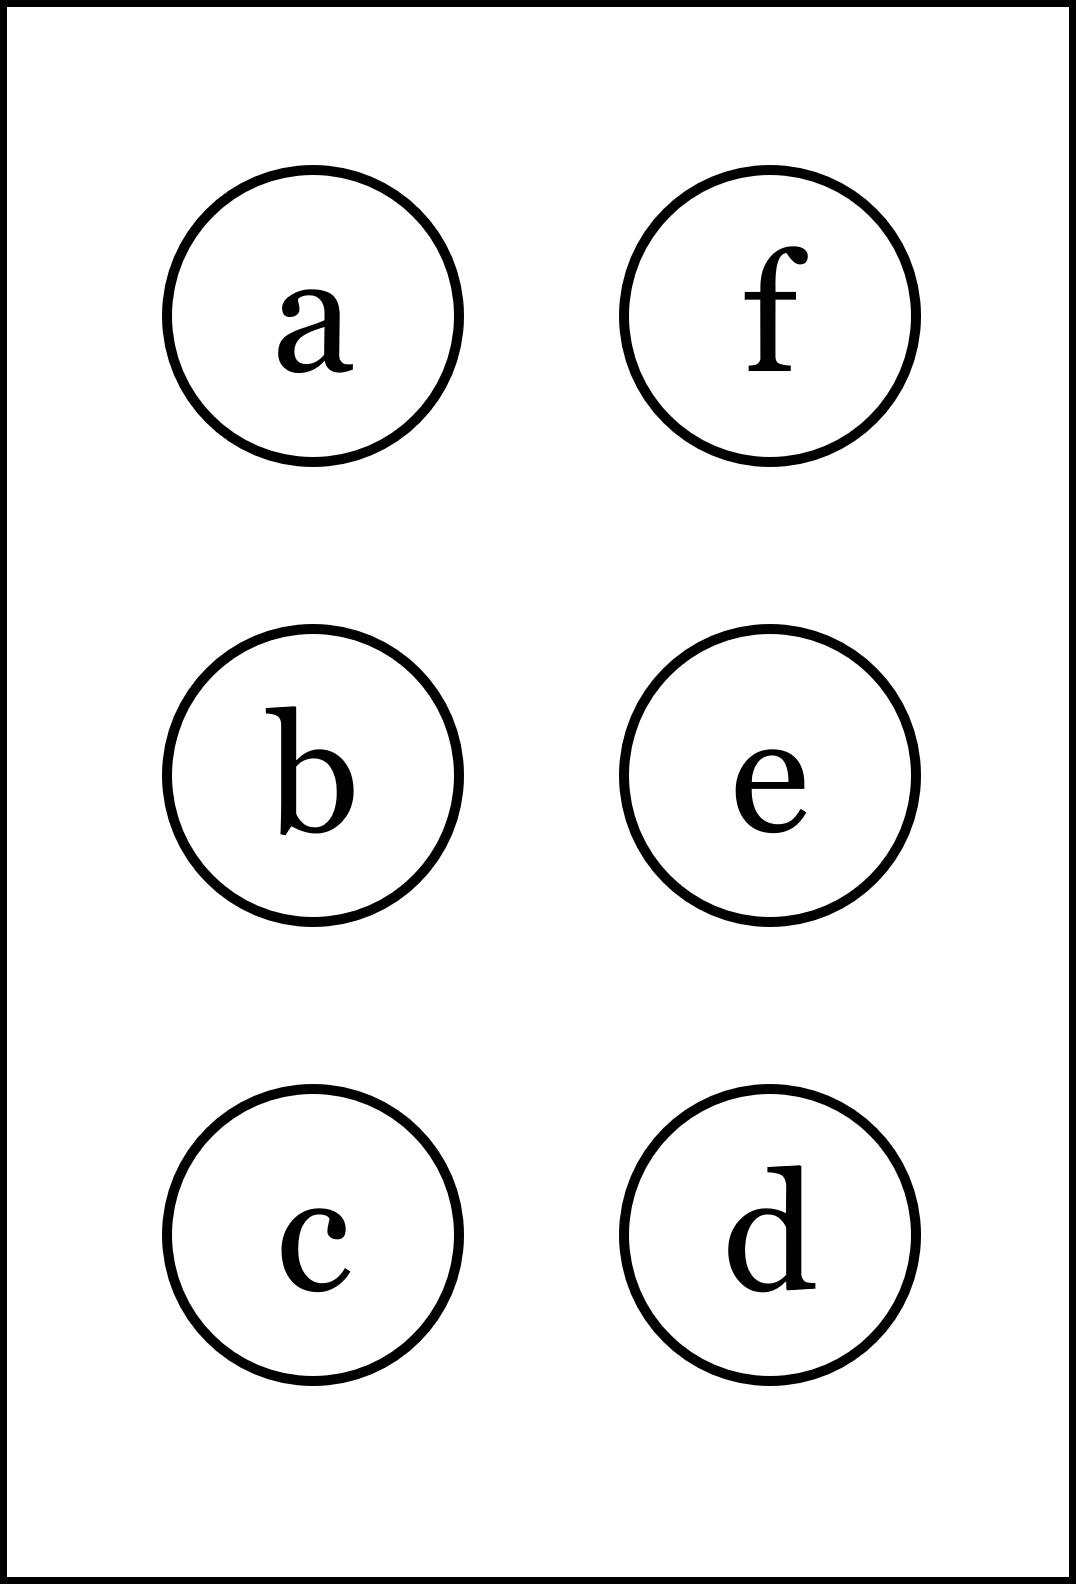
\includegraphics[height=40mm]{../images/braille.png}
{\small Písmeno Braillovej abecedy}
\end{center}
\end{minipage}
\end{center}
\end{minipage}
%
\end{tabular}
\newpage
\thispagestyle{empty}
\begin{tabular}{c:c}
\begin{minipage}[c][104.5mm][t]{0.5\linewidth}
\begin{center}
\vspace{7mm}
{\huge Tečna funkce, skupina \textit{Nu $\nu$} -\romannumeral1}\\[5mm]
\textit{Meno:}\phantom{xxxxxxxxxxxxxxxxxxxxxxxxxxxxxxxxxxxxxxxxxxxxxxxxxxxxxxxxxxxxxxxxx}\\[5mm]
\begin{minipage}{0.95\linewidth}
\begin{center}
V \textbf{(a)} a \textbf{(b)} urči \text{rovnicu tečny} $y = kx + q$ ku funkci $f(x)$ v bode $x_0$.\\V \textbf{(c)} a \textbf{(d)} urči ypsilonové souřadnice bodů, ve kterých je sklon $f(x)$ rovný $k$.\\Pokud se výsledky shodujú s těmi za otazníky, tak napravo obarvi\\příslušející kroužek načerno. \textbf{Spolu odevzdejte výsledné slovo}.
\end{center}
\end{minipage}
\\[1mm]
\begin{minipage}{0.79\linewidth}
\begin{center}
\begin{varwidth}{\linewidth}
\begin{enumerate}
\small
\item $f(x)=\cfrac{-2x-4}{-6x-3}\enspace , \enspace x_0=-1$\quad \dotfill\; ???\;\dotfill \quad $y = -2x-\frac{8}{3}$
\item $f(x)=-3\sqrt{-6x+3}\enspace , \enspace x_0=\frac{1}{3}$\quad \dotfill\; ???\;\dotfill \quad $y = 9x-6$
\item $f(x)=5x^2-4x-6\enspace , \enspace k=2$\quad \dotfill\; ???\;\dotfill \quad $-\frac{33}{5}$
\item $f(x)=4x^3-24x^2-56x+4\enspace , \enspace k=4$\quad \dotfill\; ???\;\dotfill \quad $32 , 184$
\item \quad \dotfill\; ???\;\dotfill \quad vybarvi
\item \quad \dotfill\; ???\;\dotfill \quad nebarvi
\end{enumerate}
\end{varwidth}
\end{center}
\end{minipage}
\begin{minipage}{0.20\linewidth}
\begin{center}
{\Huge\bfseries 1.} \\[2mm]
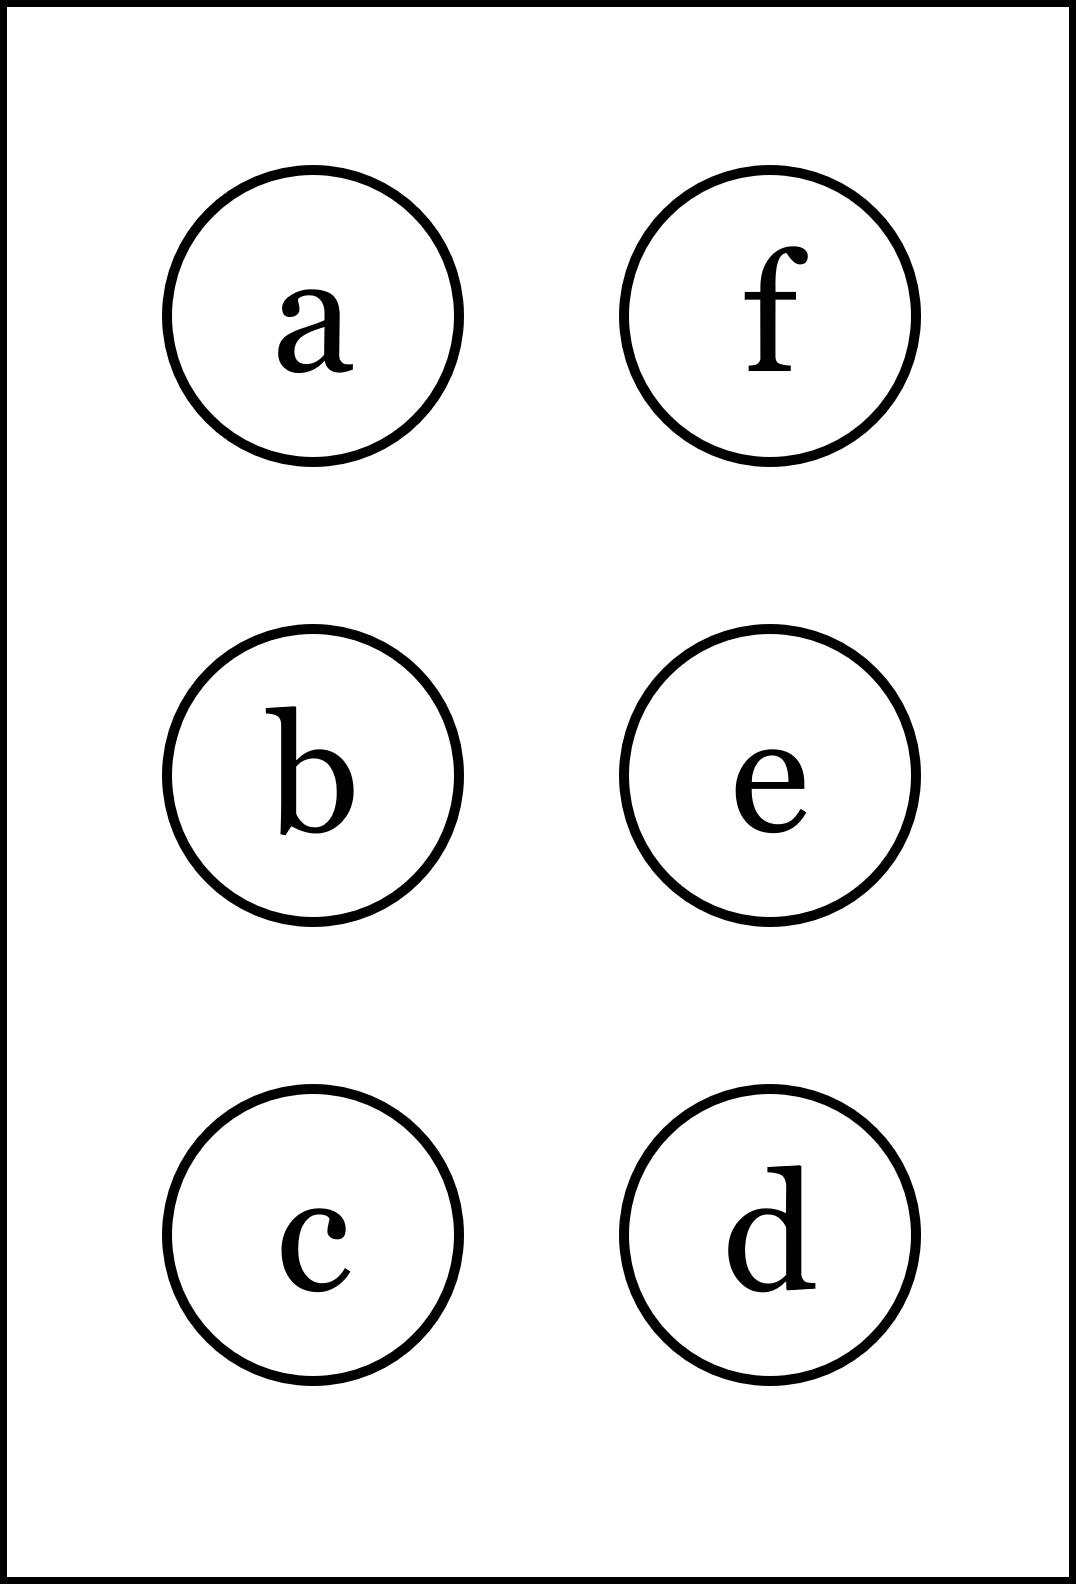
\includegraphics[height=40mm]{../images/braille.png}
{\small Písmeno Braillovej abecedy}
\end{center}
\end{minipage}
\end{center}
\end{minipage}
&
\begin{minipage}[c][104.5mm][t]{0.5\linewidth}
\begin{center}
\vspace{7mm}
{\huge Tečna funkce, skupina \textit{Nu $\nu$} -\romannumeral2}\\[5mm]
\textit{Meno:}\phantom{xxxxxxxxxxxxxxxxxxxxxxxxxxxxxxxxxxxxxxxxxxxxxxxxxxxxxxxxxxxxxxxxx}\\[5mm]
\begin{minipage}{0.95\linewidth}
\begin{center}
V \textbf{(a)} a \textbf{(b)} urči \text{rovnicu tečny} $y = kx + q$ ku funkci $f(x)$ v bode $x_0$.\\V \textbf{(c)} a \textbf{(d)} urči ypsilonové souřadnice bodů, ve kterých je sklon $f(x)$ rovný $k$.\\Pokud se výsledky shodujú s těmi za otazníky, tak napravo obarvi\\příslušející kroužek načerno. \textbf{Spolu odevzdejte výsledné slovo}.
\end{center}
\end{minipage}
\\[1mm]
\begin{minipage}{0.79\linewidth}
\begin{center}
\begin{varwidth}{\linewidth}
\begin{enumerate}
\small
\item $f(x)=\cfrac{2x-7}{-x-5}\enspace , \enspace x_0=4$\quad \dotfill\; ???\;\dotfill \quad $y = -\frac{17}{81}x+\frac{59}{81}$
\item $f(x)=5\sqrt{x-3}\enspace , \enspace x_0=4$\quad \dotfill\; ???\;\dotfill \quad $y = \frac{5}{2}x-10$
\item $f(x)=4x^2-4x+3\enspace , \enspace k=-2$\quad \dotfill\; ???\;\dotfill \quad $\frac{9}{4}$
\item $f(x)=x^3-9x^2-25x+1\enspace , \enspace k=-4$\quad \dotfill\; ???\;\dotfill \quad $16 , 78$
\item \quad \dotfill\; ???\;\dotfill \quad vybarvi
\item \quad \dotfill\; ???\;\dotfill \quad nebarvi
\end{enumerate}
\end{varwidth}
\end{center}
\end{minipage}
\begin{minipage}{0.20\linewidth}
\begin{center}
{\Huge\bfseries 2.} \\[2mm]
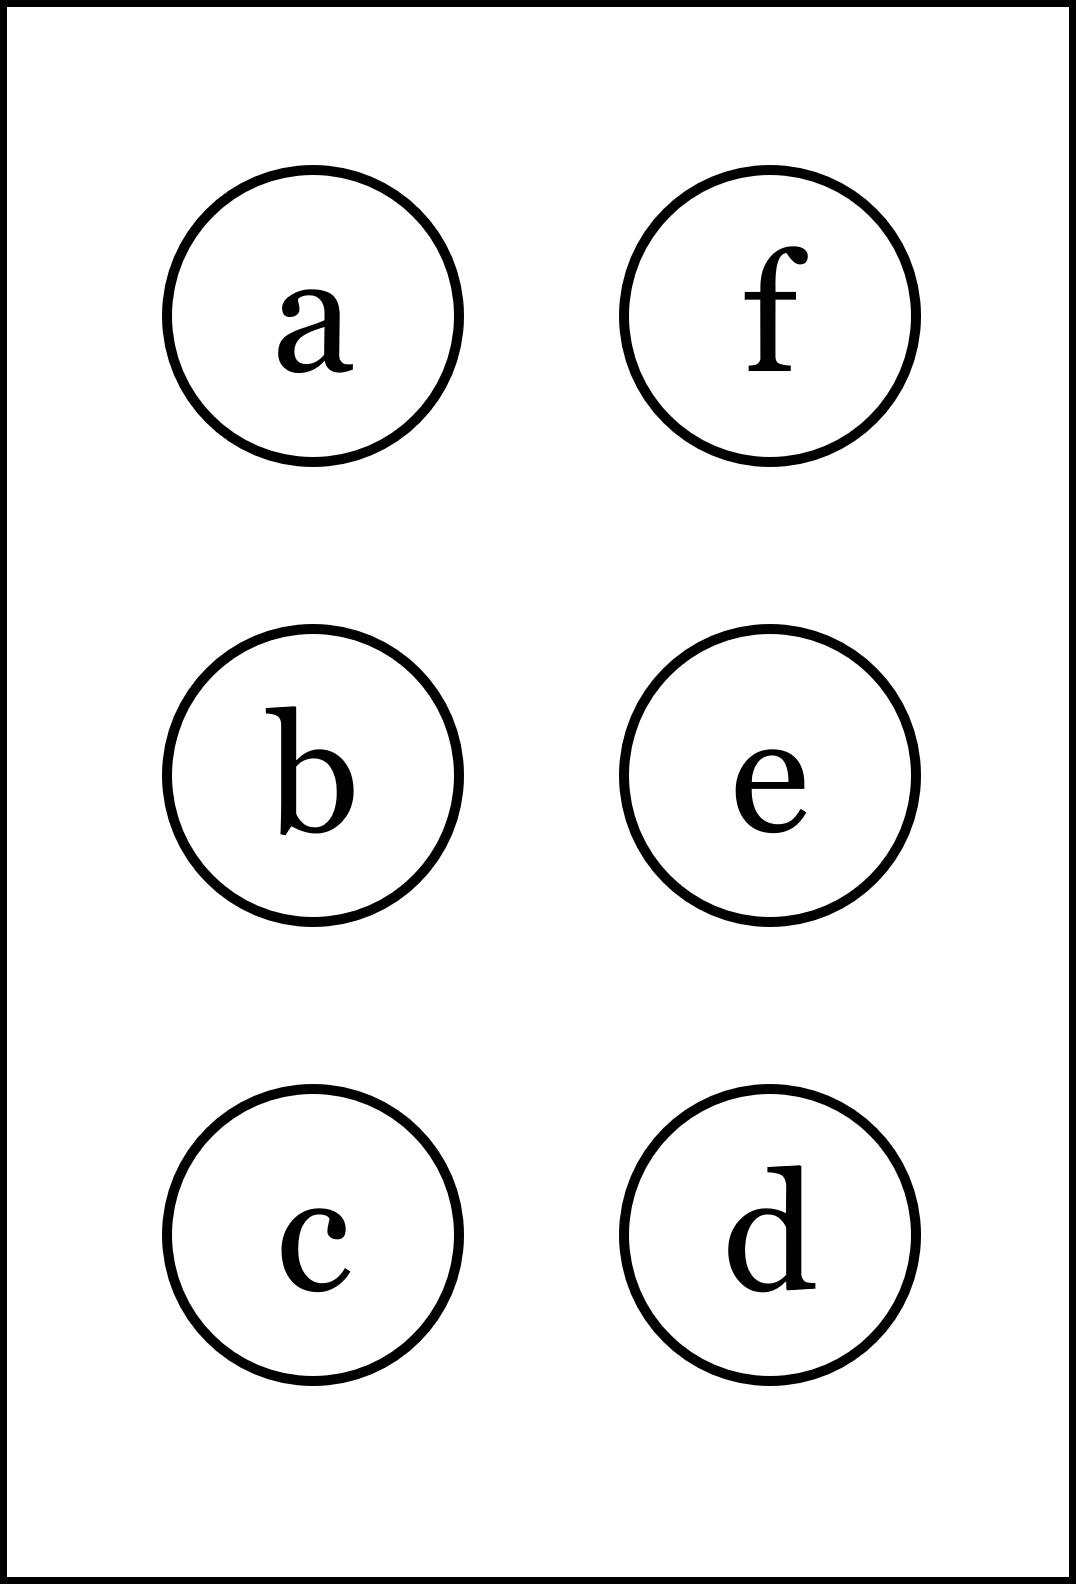
\includegraphics[height=40mm]{../images/braille.png}
{\small Písmeno Braillovej abecedy}
\end{center}
\end{minipage}
\end{center}
\end{minipage}
\\ \hdashline
\begin{minipage}[c][104.5mm][t]{0.5\linewidth}
\begin{center}
\vspace{7mm}
{\huge Tečna funkce, skupina \textit{Nu $\nu$} -\romannumeral3}\\[5mm]
\textit{Meno:}\phantom{xxxxxxxxxxxxxxxxxxxxxxxxxxxxxxxxxxxxxxxxxxxxxxxxxxxxxxxxxxxxxxxxx}\\[5mm]
\begin{minipage}{0.95\linewidth}
\begin{center}
V \textbf{(a)} a \textbf{(b)} urči \text{rovnicu tečny} $y = kx + q$ ku funkci $f(x)$ v bode $x_0$.\\V \textbf{(c)} a \textbf{(d)} urči ypsilonové souřadnice bodů, ve kterých je sklon $f(x)$ rovný $k$.\\Pokud se výsledky shodujú s těmi za otazníky, tak napravo obarvi\\příslušející kroužek načerno. \textbf{Spolu odevzdejte výsledné slovo}.
\end{center}
\end{minipage}
\\[1mm]
\begin{minipage}{0.79\linewidth}
\begin{center}
\begin{varwidth}{\linewidth}
\begin{enumerate}
\small
\item $f(x)=\cfrac{-2x+6}{-x+4}\enspace , \enspace x_0=2$\quad \dotfill\; ???\;\dotfill \quad $y = -\frac{1}{2}x+2$
\item $f(x)=-4\sqrt{-2x+7}\enspace , \enspace x_0=3$\quad \dotfill\; ???\;\dotfill \quad $y = 4x-16$
\item $f(x)=-5x^2+2x-6\enspace , \enspace k=-4$\quad \dotfill\; ???\;\dotfill \quad $-\frac{33}{5}$
\item $f(x)=4x^3-12x^2-40x+4\enspace , \enspace k=-4$\quad \dotfill\; ???\;\dotfill \quad $28 , 124$
\item \quad \dotfill\; ???\;\dotfill \quad nebarvi
\item \quad \dotfill\; ???\;\dotfill \quad vybarvi
\end{enumerate}
\end{varwidth}
\end{center}
\end{minipage}
\begin{minipage}{0.20\linewidth}
\begin{center}
{\Huge\bfseries 3.} \\[2mm]
\includegraphics[height=40mm]{../images/braille.png}
{\small Písmeno Braillovej abecedy}
\end{center}
\end{minipage}
\end{center}
\end{minipage}
&
\begin{minipage}[c][104.5mm][t]{0.5\linewidth}
\begin{center}
\vspace{7mm}
{\huge Tečna funkce, skupina \textit{Nu $\nu$} -\romannumeral4}\\[5mm]
\textit{Meno:}\phantom{xxxxxxxxxxxxxxxxxxxxxxxxxxxxxxxxxxxxxxxxxxxxxxxxxxxxxxxxxxxxxxxxx}\\[5mm]
\begin{minipage}{0.95\linewidth}
\begin{center}
V \textbf{(a)} a \textbf{(b)} urči \text{rovnicu tečny} $y = kx + q$ ku funkci $f(x)$ v bode $x_0$.\\V \textbf{(c)} a \textbf{(d)} urči ypsilonové souřadnice bodů, ve kterých je sklon $f(x)$ rovný $k$.\\Pokud se výsledky shodujú s těmi za otazníky, tak napravo obarvi\\příslušející kroužek načerno. \textbf{Spolu odevzdejte výsledné slovo}.
\end{center}
\end{minipage}
\\[1mm]
\begin{minipage}{0.79\linewidth}
\begin{center}
\begin{varwidth}{\linewidth}
\begin{enumerate}
\small
\item $f(x)=\cfrac{-2x+5}{-3x-3}\enspace , \enspace x_0=-3$\quad \dotfill\; ???\;\dotfill \quad $y = \frac{7}{12}x+\frac{43}{12}$
\item $f(x)=4\sqrt{-2x-2}\enspace , \enspace x_0=-3$\quad \dotfill\; ???\;\dotfill \quad $y = -2x+4$
\item $f(x)=9x^2+7x-2\enspace , \enspace k=-6$\quad \dotfill\; ???\;\dotfill \quad $\frac{59}{36}$
\item $f(x)=x^3-3x^2-49x-5\enspace , \enspace k=-4$\quad \dotfill\; ???\;\dotfill \quad $88 , 290$
\item \quad \dotfill\; ???\;\dotfill \quad nebarvi
\item \quad \dotfill\; ???\;\dotfill \quad nebarvi
\end{enumerate}
\end{varwidth}
\end{center}
\end{minipage}
\begin{minipage}{0.20\linewidth}
\begin{center}
{\Huge\bfseries 4.} \\[2mm]
\includegraphics[height=40mm]{../images/braille.png}
{\small Písmeno Braillovej abecedy}
\end{center}
\end{minipage}
\end{center}
\end{minipage}
%
\end{tabular}
\newpage
\thispagestyle{empty}
\begin{tabular}{c:c}
\begin{minipage}[c][104.5mm][t]{0.5\linewidth}
\begin{center}
\vspace{7mm}
{\huge Tečna funkce, skupina \textit{Xi $\xi$} -\romannumeral1}\\[5mm]
\textit{Meno:}\phantom{xxxxxxxxxxxxxxxxxxxxxxxxxxxxxxxxxxxxxxxxxxxxxxxxxxxxxxxxxxxxxxxxx}\\[5mm]
\begin{minipage}{0.95\linewidth}
\begin{center}
V \textbf{(a)} a \textbf{(b)} urči \text{rovnicu tečny} $y = kx + q$ ku funkci $f(x)$ v bode $x_0$.\\V \textbf{(c)} a \textbf{(d)} urči ypsilonové souřadnice bodů, ve kterých je sklon $f(x)$ rovný $k$.\\Pokud se výsledky shodujú s těmi za otazníky, tak napravo obarvi\\příslušející kroužek načerno. \textbf{Spolu odevzdejte výsledné slovo}.
\end{center}
\end{minipage}
\\[1mm]
\begin{minipage}{0.79\linewidth}
\begin{center}
\begin{varwidth}{\linewidth}
\begin{enumerate}
\small
\item $f(x)=\cfrac{-x+1}{x+2}\enspace , \enspace x_0=3$\quad \dotfill\; ???\;\dotfill \quad $y = -\frac{3}{25}x-\frac{1}{25}$
\item $f(x)=-3\sqrt{-6x+3}\enspace , \enspace x_0=-\frac{1}{6}$\quad \dotfill\; ???\;\dotfill \quad $y = \frac{9}{2}x-\frac{21}{4}$
\item $f(x)=2x^2+6x-5\enspace , \enspace k=-5$\quad \dotfill\; ???\;\dotfill \quad $-\frac{51}{8}$
\item $f(x)=3x^3-9x^2-24x-5\enspace , \enspace k=3$\quad \dotfill\; ???\;\dotfill \quad $7 , -77$
\item \quad \dotfill\; ???\;\dotfill \quad nebarvi
\item \quad \dotfill\; ???\;\dotfill \quad nebarvi
\end{enumerate}
\end{varwidth}
\end{center}
\end{minipage}
\begin{minipage}{0.20\linewidth}
\begin{center}
{\Huge\bfseries 1.} \\[2mm]
\includegraphics[height=40mm]{../images/braille.png}
{\small Písmeno Braillovej abecedy}
\end{center}
\end{minipage}
\end{center}
\end{minipage}
&
\begin{minipage}[c][104.5mm][t]{0.5\linewidth}
\begin{center}
\vspace{7mm}
{\huge Tečna funkce, skupina \textit{Xi $\xi$} -\romannumeral2}\\[5mm]
\textit{Meno:}\phantom{xxxxxxxxxxxxxxxxxxxxxxxxxxxxxxxxxxxxxxxxxxxxxxxxxxxxxxxxxxxxxxxxx}\\[5mm]
\begin{minipage}{0.95\linewidth}
\begin{center}
V \textbf{(a)} a \textbf{(b)} urči \text{rovnicu tečny} $y = kx + q$ ku funkci $f(x)$ v bode $x_0$.\\V \textbf{(c)} a \textbf{(d)} urči ypsilonové souřadnice bodů, ve kterých je sklon $f(x)$ rovný $k$.\\Pokud se výsledky shodujú s těmi za otazníky, tak napravo obarvi\\příslušející kroužek načerno. \textbf{Spolu odevzdejte výsledné slovo}.
\end{center}
\end{minipage}
\\[1mm]
\begin{minipage}{0.79\linewidth}
\begin{center}
\begin{varwidth}{\linewidth}
\begin{enumerate}
\small
\item $f(x)=\cfrac{9x-2}{3x+3}\enspace , \enspace x_0=1$\quad \dotfill\; ???\;\dotfill \quad $y = \frac{11}{12}x+\frac{1}{4}$
\item $f(x)=-8\sqrt{7x-4}\enspace , \enspace x_0=\frac{5}{7}$\quad \dotfill\; ???\;\dotfill \quad $y = -28x+24$
\item $f(x)=2x^2+5x+8\enspace , \enspace k=-2$\quad \dotfill\; ???\;\dotfill \quad $-\frac{85}{8}$
\item $f(x)=2x^3-12x^2-28x-5\enspace , \enspace k=2$\quad \dotfill\; ???\;\dotfill \quad $9 , 85$
\item \quad \dotfill\; ???\;\dotfill \quad nebarvi
\item \quad \dotfill\; ???\;\dotfill \quad nebarvi
\end{enumerate}
\end{varwidth}
\end{center}
\end{minipage}
\begin{minipage}{0.20\linewidth}
\begin{center}
{\Huge\bfseries 2.} \\[2mm]
\includegraphics[height=40mm]{../images/braille.png}
{\small Písmeno Braillovej abecedy}
\end{center}
\end{minipage}
\end{center}
\end{minipage}
\\ \hdashline
\begin{minipage}[c][104.5mm][t]{0.5\linewidth}
\begin{center}
\vspace{7mm}
{\huge Tečna funkce, skupina \textit{Xi $\xi$} -\romannumeral3}\\[5mm]
\textit{Meno:}\phantom{xxxxxxxxxxxxxxxxxxxxxxxxxxxxxxxxxxxxxxxxxxxxxxxxxxxxxxxxxxxxxxxxx}\\[5mm]
\begin{minipage}{0.95\linewidth}
\begin{center}
V \textbf{(a)} a \textbf{(b)} urči \text{rovnicu tečny} $y = kx + q$ ku funkci $f(x)$ v bode $x_0$.\\V \textbf{(c)} a \textbf{(d)} urči ypsilonové souřadnice bodů, ve kterých je sklon $f(x)$ rovný $k$.\\Pokud se výsledky shodujú s těmi za otazníky, tak napravo obarvi\\příslušející kroužek načerno. \textbf{Spolu odevzdejte výsledné slovo}.
\end{center}
\end{minipage}
\\[1mm]
\begin{minipage}{0.79\linewidth}
\begin{center}
\begin{varwidth}{\linewidth}
\begin{enumerate}
\small
\item $f(x)=\cfrac{x-9}{x-6}\enspace , \enspace x_0=-4$\quad \dotfill\; ???\;\dotfill \quad $y = \frac{3}{100}x+\frac{71}{50}$
\item $f(x)=6\sqrt{-3x-1}\enspace , \enspace x_0=-\frac{17}{3}$\quad \dotfill\; ???\;\dotfill \quad $y = -\frac{9}{4}x+\frac{45}{2}$
\item $f(x)=-3x^2-x-2\enspace , \enspace k=-8$\quad \dotfill\; ???\;\dotfill \quad $-\frac{29}{4}$
\item $f(x)=x^3-9x^2+23x+3\enspace , \enspace k=-1$\quad \dotfill\; ???\;\dotfill \quad $21 , -169$
\item \quad \dotfill\; ???\;\dotfill \quad vybarvi
\item \quad \dotfill\; ???\;\dotfill \quad vybarvi
\end{enumerate}
\end{varwidth}
\end{center}
\end{minipage}
\begin{minipage}{0.20\linewidth}
\begin{center}
{\Huge\bfseries 3.} \\[2mm]
\includegraphics[height=40mm]{../images/braille.png}
{\small Písmeno Braillovej abecedy}
\end{center}
\end{minipage}
\end{center}
\end{minipage}
&
\begin{minipage}[c][104.5mm][t]{0.5\linewidth}
\begin{center}
\vspace{7mm}
{\huge Tečna funkce, skupina \textit{Xi $\xi$} -\romannumeral4}\\[5mm]
\textit{Meno:}\phantom{xxxxxxxxxxxxxxxxxxxxxxxxxxxxxxxxxxxxxxxxxxxxxxxxxxxxxxxxxxxxxxxxx}\\[5mm]
\begin{minipage}{0.95\linewidth}
\begin{center}
V \textbf{(a)} a \textbf{(b)} urči \text{rovnicu tečny} $y = kx + q$ ku funkci $f(x)$ v bode $x_0$.\\V \textbf{(c)} a \textbf{(d)} urči ypsilonové souřadnice bodů, ve kterých je sklon $f(x)$ rovný $k$.\\Pokud se výsledky shodujú s těmi za otazníky, tak napravo obarvi\\příslušející kroužek načerno. \textbf{Spolu odevzdejte výsledné slovo}.
\end{center}
\end{minipage}
\\[1mm]
\begin{minipage}{0.79\linewidth}
\begin{center}
\begin{varwidth}{\linewidth}
\begin{enumerate}
\small
\item $f(x)=\cfrac{-3x+5}{-4x-3}\enspace , \enspace x_0=2$\quad \dotfill\; ???\;\dotfill \quad $y = \frac{29}{121}x-\frac{47}{121}$
\item $f(x)=3\sqrt{4x+3}\enspace , \enspace x_0=\frac{13}{4}$\quad \dotfill\; ???\;\dotfill \quad $y = \frac{3}{2}x+\frac{57}{4}$
\item $f(x)=5x^2+x+9\enspace , \enspace k=-1$\quad \dotfill\; ???\;\dotfill \quad $-9$
\item $f(x)=x^3-9x^2-78x-5\enspace , \enspace k=3$\quad \dotfill\; ???\;\dotfill \quad $121 , 697$
\item \quad \dotfill\; ???\;\dotfill \quad nebarvi
\item \quad \dotfill\; ???\;\dotfill \quad nebarvi
\end{enumerate}
\end{varwidth}
\end{center}
\end{minipage}
\begin{minipage}{0.20\linewidth}
\begin{center}
{\Huge\bfseries 4.} \\[2mm]
\includegraphics[height=40mm]{../images/braille.png}
{\small Písmeno Braillovej abecedy}
\end{center}
\end{minipage}
\end{center}
\end{minipage}
%
\end{tabular}
\newpage
\thispagestyle{empty}
\begin{tabular}{c:c}
\begin{minipage}[c][104.5mm][t]{0.5\linewidth}
\begin{center}
\vspace{7mm}
{\huge Tečna funkce, skupina \textit{Omicron $\omicron$} -\romannumeral1}\\[5mm]
\textit{Meno:}\phantom{xxxxxxxxxxxxxxxxxxxxxxxxxxxxxxxxxxxxxxxxxxxxxxxxxxxxxxxxxxxxxxxxx}\\[5mm]
\begin{minipage}{0.95\linewidth}
\begin{center}
V \textbf{(a)} a \textbf{(b)} urči \text{rovnicu tečny} $y = kx + q$ ku funkci $f(x)$ v bode $x_0$.\\V \textbf{(c)} a \textbf{(d)} urči ypsilonové souřadnice bodů, ve kterých je sklon $f(x)$ rovný $k$.\\Pokud se výsledky shodujú s těmi za otazníky, tak napravo obarvi\\příslušející kroužek načerno. \textbf{Spolu odevzdejte výsledné slovo}.
\end{center}
\end{minipage}
\\[1mm]
\begin{minipage}{0.79\linewidth}
\begin{center}
\begin{varwidth}{\linewidth}
\begin{enumerate}
\small
\item $f(x)=\cfrac{3x-8}{2x-1}\enspace , \enspace x_0=1$\quad \dotfill\; ???\;\dotfill \quad $y = 13x-18$
\item $f(x)=-6\sqrt{x+7}\enspace , \enspace x_0=29$\quad \dotfill\; ???\;\dotfill \quad $y = -\frac{1}{2}x-\frac{43}{2}$
\item $f(x)=6x^2-2x-3\enspace , \enspace k=-4$\quad \dotfill\; ???\;\dotfill \quad $-\frac{5}{2}$
\item $f(x)=x^3-6x^2+11x+2\enspace , \enspace k=2$\quad \dotfill\; ???\;\dotfill \quad $8 , -58$
\item \quad \dotfill\; ???\;\dotfill \quad vybarvi
\item \quad \dotfill\; ???\;\dotfill \quad nebarvi
\end{enumerate}
\end{varwidth}
\end{center}
\end{minipage}
\begin{minipage}{0.20\linewidth}
\begin{center}
{\Huge\bfseries 1.} \\[2mm]
\includegraphics[height=40mm]{../images/braille.png}
{\small Písmeno Braillovej abecedy}
\end{center}
\end{minipage}
\end{center}
\end{minipage}
&
\begin{minipage}[c][104.5mm][t]{0.5\linewidth}
\begin{center}
\vspace{7mm}
{\huge Tečna funkce, skupina \textit{Omicron $\omicron$} -\romannumeral2}\\[5mm]
\textit{Meno:}\phantom{xxxxxxxxxxxxxxxxxxxxxxxxxxxxxxxxxxxxxxxxxxxxxxxxxxxxxxxxxxxxxxxxx}\\[5mm]
\begin{minipage}{0.95\linewidth}
\begin{center}
V \textbf{(a)} a \textbf{(b)} urči \text{rovnicu tečny} $y = kx + q$ ku funkci $f(x)$ v bode $x_0$.\\V \textbf{(c)} a \textbf{(d)} urči ypsilonové souřadnice bodů, ve kterých je sklon $f(x)$ rovný $k$.\\Pokud se výsledky shodujú s těmi za otazníky, tak napravo obarvi\\příslušející kroužek načerno. \textbf{Spolu odevzdejte výsledné slovo}.
\end{center}
\end{minipage}
\\[1mm]
\begin{minipage}{0.79\linewidth}
\begin{center}
\begin{varwidth}{\linewidth}
\begin{enumerate}
\small
\item $f(x)=\cfrac{-x-6}{-x-9}\enspace , \enspace x_0=-7$\quad \dotfill\; ???\;\dotfill \quad $y = \frac{3}{4}x+\frac{19}{4}$
\item $f(x)=-2\sqrt{6x+3}\enspace , \enspace x_0=1$\quad \dotfill\; ???\;\dotfill \quad $y = -2x-8$
\item $f(x)=8x^2+9x+3\enspace , \enspace k=3$\quad \dotfill\; ???\;\dotfill \quad $\frac{3}{4}$
\item $f(x)=x^3-3x^2-46x+5\enspace , \enspace k=-1$\quad \dotfill\; ???\;\dotfill \quad $89 , -175$
\item \quad \dotfill\; ???\;\dotfill \quad vybarvi
\item \quad \dotfill\; ???\;\dotfill \quad vybarvi
\end{enumerate}
\end{varwidth}
\end{center}
\end{minipage}
\begin{minipage}{0.20\linewidth}
\begin{center}
{\Huge\bfseries 2.} \\[2mm]
\includegraphics[height=40mm]{../images/braille.png}
{\small Písmeno Braillovej abecedy}
\end{center}
\end{minipage}
\end{center}
\end{minipage}
\\ \hdashline
\begin{minipage}[c][104.5mm][t]{0.5\linewidth}
\begin{center}
\vspace{7mm}
{\huge Tečna funkce, skupina \textit{Omicron $\omicron$} -\romannumeral3}\\[5mm]
\textit{Meno:}\phantom{xxxxxxxxxxxxxxxxxxxxxxxxxxxxxxxxxxxxxxxxxxxxxxxxxxxxxxxxxxxxxxxxx}\\[5mm]
\begin{minipage}{0.95\linewidth}
\begin{center}
V \textbf{(a)} a \textbf{(b)} urči \text{rovnicu tečny} $y = kx + q$ ku funkci $f(x)$ v bode $x_0$.\\V \textbf{(c)} a \textbf{(d)} urči ypsilonové souřadnice bodů, ve kterých je sklon $f(x)$ rovný $k$.\\Pokud se výsledky shodujú s těmi za otazníky, tak napravo obarvi\\příslušející kroužek načerno. \textbf{Spolu odevzdejte výsledné slovo}.
\end{center}
\end{minipage}
\\[1mm]
\begin{minipage}{0.79\linewidth}
\begin{center}
\begin{varwidth}{\linewidth}
\begin{enumerate}
\small
\item $f(x)=\cfrac{-x+7}{x+2}\enspace , \enspace x_0=-6$\quad \dotfill\; ???\;\dotfill \quad $y = -\frac{9}{16}x-\frac{53}{8}$
\item $f(x)=-\sqrt{-4x-4}\enspace , \enspace x_0=-10$\quad \dotfill\; ???\;\dotfill \quad $y = \frac{1}{3}x-\frac{8}{3}$
\item $f(x)=6x^2+7x+7\enspace , \enspace k=2$\quad \dotfill\; ???\;\dotfill \quad $-\frac{71}{8}$
\item $f(x)=2x^3-6x^2-17x+2\enspace , \enspace k=1$\quad \dotfill\; ???\;\dotfill \quad $11 , 53$
\item \quad \dotfill\; ???\;\dotfill \quad nebarvi
\item \quad \dotfill\; ???\;\dotfill \quad nebarvi
\end{enumerate}
\end{varwidth}
\end{center}
\end{minipage}
\begin{minipage}{0.20\linewidth}
\begin{center}
{\Huge\bfseries 3.} \\[2mm]
\includegraphics[height=40mm]{../images/braille.png}
{\small Písmeno Braillovej abecedy}
\end{center}
\end{minipage}
\end{center}
\end{minipage}
&
\begin{minipage}[c][104.5mm][t]{0.5\linewidth}
\begin{center}
\vspace{7mm}
{\huge Tečna funkce, skupina \textit{Omicron $\omicron$} -\romannumeral4}\\[5mm]
\textit{Meno:}\phantom{xxxxxxxxxxxxxxxxxxxxxxxxxxxxxxxxxxxxxxxxxxxxxxxxxxxxxxxxxxxxxxxxx}\\[5mm]
\begin{minipage}{0.95\linewidth}
\begin{center}
V \textbf{(a)} a \textbf{(b)} urči \text{rovnicu tečny} $y = kx + q$ ku funkci $f(x)$ v bode $x_0$.\\V \textbf{(c)} a \textbf{(d)} urči ypsilonové souřadnice bodů, ve kterých je sklon $f(x)$ rovný $k$.\\Pokud se výsledky shodujú s těmi za otazníky, tak napravo obarvi\\příslušející kroužek načerno. \textbf{Spolu odevzdejte výsledné slovo}.
\end{center}
\end{minipage}
\\[1mm]
\begin{minipage}{0.79\linewidth}
\begin{center}
\begin{varwidth}{\linewidth}
\begin{enumerate}
\small
\item $f(x)=\cfrac{4x-3}{4x-7}\enspace , \enspace x_0=-1$\quad \dotfill\; ???\;\dotfill \quad $y = -\frac{16}{121}x+\frac{61}{121}$
\item $f(x)=4\sqrt{2x-5}\enspace , \enspace x_0=\frac{9}{2}$\quad \dotfill\; ???\;\dotfill \quad $y = 2x-2$
\item $f(x)=x^2+x-1\enspace , \enspace k=6$\quad \dotfill\; ???\;\dotfill \quad $\frac{39}{4}$
\item $f(x)=3x^3-9x^2-29x-1\enspace , \enspace k=-2$\quad \dotfill\; ???\;\dotfill \quad $16 , 86$
\item \quad \dotfill\; ???\;\dotfill \quad nebarvi
\item \quad \dotfill\; ???\;\dotfill \quad nebarvi
\end{enumerate}
\end{varwidth}
\end{center}
\end{minipage}
\begin{minipage}{0.20\linewidth}
\begin{center}
{\Huge\bfseries 4.} \\[2mm]
\includegraphics[height=40mm]{../images/braille.png}
{\small Písmeno Braillovej abecedy}
\end{center}
\end{minipage}
\end{center}
\end{minipage}
%
\end{tabular}
\newpage
\thispagestyle{empty}
\begin{tabular}{c:c}
\begin{minipage}[c][104.5mm][t]{0.5\linewidth}
\begin{center}
\vspace{7mm}
{\huge Tečna funkce, skupina \textit{Pi $\pi$} -\romannumeral1}\\[5mm]
\textit{Meno:}\phantom{xxxxxxxxxxxxxxxxxxxxxxxxxxxxxxxxxxxxxxxxxxxxxxxxxxxxxxxxxxxxxxxxx}\\[5mm]
\begin{minipage}{0.95\linewidth}
\begin{center}
V \textbf{(a)} a \textbf{(b)} urči \text{rovnicu tečny} $y = kx + q$ ku funkci $f(x)$ v bode $x_0$.\\V \textbf{(c)} a \textbf{(d)} urči ypsilonové souřadnice bodů, ve kterých je sklon $f(x)$ rovný $k$.\\Pokud se výsledky shodujú s těmi za otazníky, tak napravo obarvi\\příslušející kroužek načerno. \textbf{Spolu odevzdejte výsledné slovo}.
\end{center}
\end{minipage}
\\[1mm]
\begin{minipage}{0.79\linewidth}
\begin{center}
\begin{varwidth}{\linewidth}
\begin{enumerate}
\small
\item $f(x)=\cfrac{-6x+4}{8x+1}\enspace , \enspace x_0=-1$\quad \dotfill\; ???\;\dotfill \quad $y = -\frac{38}{49}x-\frac{108}{49}$
\item $f(x)=5\sqrt{3x+6}\enspace , \enspace x_0=\frac{19}{3}$\quad \dotfill\; ???\;\dotfill \quad $y = \frac{3}{2}x+31$
\item $f(x)=-x^2-4x-2\enspace , \enspace k=-6$\quad \dotfill\; ???\;\dotfill \quad $-7$
\item $f(x)=x^3-3x^2-4x-3\enspace , \enspace k=5$\quad \dotfill\; ???\;\dotfill \quad $-3 , -15$
\item \quad \dotfill\; ???\;\dotfill \quad nebarvi
\item \quad \dotfill\; ???\;\dotfill \quad nebarvi
\end{enumerate}
\end{varwidth}
\end{center}
\end{minipage}
\begin{minipage}{0.20\linewidth}
\begin{center}
{\Huge\bfseries 1.} \\[2mm]
\includegraphics[height=40mm]{../images/braille.png}
{\small Písmeno Braillovej abecedy}
\end{center}
\end{minipage}
\end{center}
\end{minipage}
&
\begin{minipage}[c][104.5mm][t]{0.5\linewidth}
\begin{center}
\vspace{7mm}
{\huge Tečna funkce, skupina \textit{Pi $\pi$} -\romannumeral2}\\[5mm]
\textit{Meno:}\phantom{xxxxxxxxxxxxxxxxxxxxxxxxxxxxxxxxxxxxxxxxxxxxxxxxxxxxxxxxxxxxxxxxx}\\[5mm]
\begin{minipage}{0.95\linewidth}
\begin{center}
V \textbf{(a)} a \textbf{(b)} urči \text{rovnicu tečny} $y = kx + q$ ku funkci $f(x)$ v bode $x_0$.\\V \textbf{(c)} a \textbf{(d)} urči ypsilonové souřadnice bodů, ve kterých je sklon $f(x)$ rovný $k$.\\Pokud se výsledky shodujú s těmi za otazníky, tak napravo obarvi\\příslušející kroužek načerno. \textbf{Spolu odevzdejte výsledné slovo}.
\end{center}
\end{minipage}
\\[1mm]
\begin{minipage}{0.79\linewidth}
\begin{center}
\begin{varwidth}{\linewidth}
\begin{enumerate}
\small
\item $f(x)=\cfrac{6x-2}{2x+3}\enspace , \enspace x_0=-1$\quad \dotfill\; ???\;\dotfill \quad $y = 22x+14$
\item $f(x)=-3\sqrt{-7x+3}\enspace , \enspace x_0=\frac{2}{7}$\quad \dotfill\; ???\;\dotfill \quad $y = \frac{21}{2}x-6$
\item $f(x)=-2x^2+9x-4\enspace , \enspace k=-5$\quad \dotfill\; ???\;\dotfill \quad $3$
\item $f(x)=2x^3-6x^2-20x+3\enspace , \enspace k=-2$\quad \dotfill\; ???\;\dotfill \quad $15 , 63$
\item \quad \dotfill\; ???\;\dotfill \quad vybarvi
\item \quad \dotfill\; ???\;\dotfill \quad nebarvi
\end{enumerate}
\end{varwidth}
\end{center}
\end{minipage}
\begin{minipage}{0.20\linewidth}
\begin{center}
{\Huge\bfseries 2.} \\[2mm]
\includegraphics[height=40mm]{../images/braille.png}
{\small Písmeno Braillovej abecedy}
\end{center}
\end{minipage}
\end{center}
\end{minipage}
\\ \hdashline
\begin{minipage}[c][104.5mm][t]{0.5\linewidth}
\begin{center}
\vspace{7mm}
{\huge Tečna funkce, skupina \textit{Pi $\pi$} -\romannumeral3}\\[5mm]
\textit{Meno:}\phantom{xxxxxxxxxxxxxxxxxxxxxxxxxxxxxxxxxxxxxxxxxxxxxxxxxxxxxxxxxxxxxxxxx}\\[5mm]
\begin{minipage}{0.95\linewidth}
\begin{center}
V \textbf{(a)} a \textbf{(b)} urči \text{rovnicu tečny} $y = kx + q$ ku funkci $f(x)$ v bode $x_0$.\\V \textbf{(c)} a \textbf{(d)} urči ypsilonové souřadnice bodů, ve kterých je sklon $f(x)$ rovný $k$.\\Pokud se výsledky shodujú s těmi za otazníky, tak napravo obarvi\\příslušející kroužek načerno. \textbf{Spolu odevzdejte výsledné slovo}.
\end{center}
\end{minipage}
\\[1mm]
\begin{minipage}{0.79\linewidth}
\begin{center}
\begin{varwidth}{\linewidth}
\begin{enumerate}
\small
\item $f(x)=\cfrac{x-1}{-5x-6}\enspace , \enspace x_0=-1$\quad \dotfill\; ???\;\dotfill \quad $y = -11x-9$
\item $f(x)=-6\sqrt{2x+8}\enspace , \enspace x_0=\frac{17}{2}$\quad \dotfill\; ???\;\dotfill \quad $y = -\frac{6}{5}x-\frac{198}{5}$
\item $f(x)=-6x^2+3x+5\enspace , \enspace k=-3$\quad \dotfill\; ???\;\dotfill \quad $-5$
\item $f(x)=4x^3-12x^2-33x+2\enspace , \enspace k=3$\quad \dotfill\; ???\;\dotfill \quad $19 , 101$
\item \quad \dotfill\; ???\;\dotfill \quad nebarvi
\item \quad \dotfill\; ???\;\dotfill \quad nebarvi
\end{enumerate}
\end{varwidth}
\end{center}
\end{minipage}
\begin{minipage}{0.20\linewidth}
\begin{center}
{\Huge\bfseries 3.} \\[2mm]
\includegraphics[height=40mm]{../images/braille.png}
{\small Písmeno Braillovej abecedy}
\end{center}
\end{minipage}
\end{center}
\end{minipage}
&
\begin{minipage}[c][104.5mm][t]{0.5\linewidth}
\begin{center}
\vspace{7mm}
{\huge Tečna funkce, skupina \textit{Pi $\pi$} -\romannumeral4}\\[5mm]
\textit{Meno:}\phantom{xxxxxxxxxxxxxxxxxxxxxxxxxxxxxxxxxxxxxxxxxxxxxxxxxxxxxxxxxxxxxxxxx}\\[5mm]
\begin{minipage}{0.95\linewidth}
\begin{center}
V \textbf{(a)} a \textbf{(b)} urči \text{rovnicu tečny} $y = kx + q$ ku funkci $f(x)$ v bode $x_0$.\\V \textbf{(c)} a \textbf{(d)} urči ypsilonové souřadnice bodů, ve kterých je sklon $f(x)$ rovný $k$.\\Pokud se výsledky shodujú s těmi za otazníky, tak napravo obarvi\\příslušející kroužek načerno. \textbf{Spolu odevzdejte výsledné slovo}.
\end{center}
\end{minipage}
\\[1mm]
\begin{minipage}{0.79\linewidth}
\begin{center}
\begin{varwidth}{\linewidth}
\begin{enumerate}
\small
\item $f(x)=\cfrac{-4x+3}{6x-1}\enspace , \enspace x_0=1$\quad \dotfill\; ???\;\dotfill \quad $y = -\frac{14}{25}x+\frac{9}{25}$
\item $f(x)=5\sqrt{4x-3}\enspace , \enspace x_0=1$\quad \dotfill\; ???\;\dotfill \quad $y = 10x-10$
\item $f(x)=x^2-8x-6\enspace , \enspace k=-5$\quad \dotfill\; ???\;\dotfill \quad $-\frac{63}{4}$
\item $f(x)=2x^3-6x^2-49x+5\enspace , \enspace k=-1$\quad \dotfill\; ???\;\dotfill \quad $63 , 233$
\item \quad \dotfill\; ???\;\dotfill \quad vybarvi
\item \quad \dotfill\; ???\;\dotfill \quad vybarvi
\end{enumerate}
\end{varwidth}
\end{center}
\end{minipage}
\begin{minipage}{0.20\linewidth}
\begin{center}
{\Huge\bfseries 4.} \\[2mm]
\includegraphics[height=40mm]{../images/braille.png}
{\small Písmeno Braillovej abecedy}
\end{center}
\end{minipage}
\end{center}
\end{minipage}
%
\end{tabular}
\newpage
\thispagestyle{empty}
\begin{tabular}{c:c}
\begin{minipage}[c][104.5mm][t]{0.5\linewidth}
\begin{center}
\vspace{7mm}
{\huge Tečna funkce, skupina \textit{Rho $\rho$} -\romannumeral1}\\[5mm]
\textit{Meno:}\phantom{xxxxxxxxxxxxxxxxxxxxxxxxxxxxxxxxxxxxxxxxxxxxxxxxxxxxxxxxxxxxxxxxx}\\[5mm]
\begin{minipage}{0.95\linewidth}
\begin{center}
V \textbf{(a)} a \textbf{(b)} urči \text{rovnicu tečny} $y = kx + q$ ku funkci $f(x)$ v bode $x_0$.\\V \textbf{(c)} a \textbf{(d)} urči ypsilonové souřadnice bodů, ve kterých je sklon $f(x)$ rovný $k$.\\Pokud se výsledky shodujú s těmi za otazníky, tak napravo obarvi\\příslušející kroužek načerno. \textbf{Spolu odevzdejte výsledné slovo}.
\end{center}
\end{minipage}
\\[1mm]
\begin{minipage}{0.79\linewidth}
\begin{center}
\begin{varwidth}{\linewidth}
\begin{enumerate}
\small
\item $f(x)=\cfrac{-4x-2}{-4x-7}\enspace , \enspace x_0=-2$\quad \dotfill\; ???\;\dotfill \quad $y = 20x+46$
\item $f(x)=5\sqrt{-x-3}\enspace , \enspace x_0=-52$\quad \dotfill\; ???\;\dotfill \quad $y = -\frac{5}{14}x+\frac{230}{7}$
\item $f(x)=-2x^2-6x-1\enspace , \enspace k=6$\quad \dotfill\; ???\;\dotfill \quad $1$
\item $f(x)=x^3-9x^2-16x-3\enspace , \enspace k=5$\quad \dotfill\; ???\;\dotfill \quad $3 , 11$
\item \quad \dotfill\; ???\;\dotfill \quad vybarvi
\item \quad \dotfill\; ???\;\dotfill \quad vybarvi
\end{enumerate}
\end{varwidth}
\end{center}
\end{minipage}
\begin{minipage}{0.20\linewidth}
\begin{center}
{\Huge\bfseries 1.} \\[2mm]
\includegraphics[height=40mm]{../images/braille.png}
{\small Písmeno Braillovej abecedy}
\end{center}
\end{minipage}
\end{center}
\end{minipage}
&
\begin{minipage}[c][104.5mm][t]{0.5\linewidth}
\begin{center}
\vspace{7mm}
{\huge Tečna funkce, skupina \textit{Rho $\rho$} -\romannumeral2}\\[5mm]
\textit{Meno:}\phantom{xxxxxxxxxxxxxxxxxxxxxxxxxxxxxxxxxxxxxxxxxxxxxxxxxxxxxxxxxxxxxxxxx}\\[5mm]
\begin{minipage}{0.95\linewidth}
\begin{center}
V \textbf{(a)} a \textbf{(b)} urči \text{rovnicu tečny} $y = kx + q$ ku funkci $f(x)$ v bode $x_0$.\\V \textbf{(c)} a \textbf{(d)} urči ypsilonové souřadnice bodů, ve kterých je sklon $f(x)$ rovný $k$.\\Pokud se výsledky shodujú s těmi za otazníky, tak napravo obarvi\\příslušející kroužek načerno. \textbf{Spolu odevzdejte výsledné slovo}.
\end{center}
\end{minipage}
\\[1mm]
\begin{minipage}{0.79\linewidth}
\begin{center}
\begin{varwidth}{\linewidth}
\begin{enumerate}
\small
\item $f(x)=\cfrac{2x-3}{x-6}\enspace , \enspace x_0=7$\quad \dotfill\; ???\;\dotfill \quad $y = -9x+74$
\item $f(x)=2\sqrt{-x+2}\enspace , \enspace x_0=1$\quad \dotfill\; ???\;\dotfill \quad $y = -x+6$
\item $f(x)=-3x^2+9x-3\enspace , \enspace k=7$\quad \dotfill\; ???\;\dotfill \quad $-\frac{1}{3}$
\item $f(x)=3x^3-9x^2-25x+4\enspace , \enspace k=2$\quad \dotfill\; ???\;\dotfill \quad $17 , 79$
\item \quad \dotfill\; ???\;\dotfill \quad vybarvi
\item \quad \dotfill\; ???\;\dotfill \quad nebarvi
\end{enumerate}
\end{varwidth}
\end{center}
\end{minipage}
\begin{minipage}{0.20\linewidth}
\begin{center}
{\Huge\bfseries 2.} \\[2mm]
\includegraphics[height=40mm]{../images/braille.png}
{\small Písmeno Braillovej abecedy}
\end{center}
\end{minipage}
\end{center}
\end{minipage}
\\ \hdashline
\begin{minipage}[c][104.5mm][t]{0.5\linewidth}
\begin{center}
\vspace{7mm}
{\huge Tečna funkce, skupina \textit{Rho $\rho$} -\romannumeral3}\\[5mm]
\textit{Meno:}\phantom{xxxxxxxxxxxxxxxxxxxxxxxxxxxxxxxxxxxxxxxxxxxxxxxxxxxxxxxxxxxxxxxxx}\\[5mm]
\begin{minipage}{0.95\linewidth}
\begin{center}
V \textbf{(a)} a \textbf{(b)} urči \text{rovnicu tečny} $y = kx + q$ ku funkci $f(x)$ v bode $x_0$.\\V \textbf{(c)} a \textbf{(d)} urči ypsilonové souřadnice bodů, ve kterých je sklon $f(x)$ rovný $k$.\\Pokud se výsledky shodujú s těmi za otazníky, tak napravo obarvi\\příslušející kroužek načerno. \textbf{Spolu odevzdejte výsledné slovo}.
\end{center}
\end{minipage}
\\[1mm]
\begin{minipage}{0.79\linewidth}
\begin{center}
\begin{varwidth}{\linewidth}
\begin{enumerate}
\small
\item $f(x)=\cfrac{-7x+6}{2x+4}\enspace , \enspace x_0=1$\quad \dotfill\; ???\;\dotfill \quad $y = -\frac{10}{9}x+\frac{17}{18}$
\item $f(x)=-3\sqrt{-2x+1}\enspace , \enspace x_0=-\frac{15}{2}$\quad \dotfill\; ???\;\dotfill \quad $y = \frac{3}{4}x-\frac{51}{8}$
\item $f(x)=4x^2-5x-2\enspace , \enspace k=4$\quad \dotfill\; ???\;\dotfill \quad $-\frac{41}{16}$
\item $f(x)=x^3-9x^2-49x-3\enspace , \enspace k=-1$\quad \dotfill\; ???\;\dotfill \quad $51 , 325$
\item \quad \dotfill\; ???\;\dotfill \quad vybarvi
\item \quad \dotfill\; ???\;\dotfill \quad nebarvi
\end{enumerate}
\end{varwidth}
\end{center}
\end{minipage}
\begin{minipage}{0.20\linewidth}
\begin{center}
{\Huge\bfseries 3.} \\[2mm]
\includegraphics[height=40mm]{../images/braille.png}
{\small Písmeno Braillovej abecedy}
\end{center}
\end{minipage}
\end{center}
\end{minipage}
&
\begin{minipage}[c][104.5mm][t]{0.5\linewidth}
\begin{center}
\vspace{7mm}
{\huge Tečna funkce, skupina \textit{Rho $\rho$} -\romannumeral4}\\[5mm]
\textit{Meno:}\phantom{xxxxxxxxxxxxxxxxxxxxxxxxxxxxxxxxxxxxxxxxxxxxxxxxxxxxxxxxxxxxxxxxx}\\[5mm]
\begin{minipage}{0.95\linewidth}
\begin{center}
V \textbf{(a)} a \textbf{(b)} urči \text{rovnicu tečny} $y = kx + q$ ku funkci $f(x)$ v bode $x_0$.\\V \textbf{(c)} a \textbf{(d)} urči ypsilonové souřadnice bodů, ve kterých je sklon $f(x)$ rovný $k$.\\Pokud se výsledky shodujú s těmi za otazníky, tak napravo obarvi\\příslušející kroužek načerno. \textbf{Spolu odevzdejte výsledné slovo}.
\end{center}
\end{minipage}
\\[1mm]
\begin{minipage}{0.79\linewidth}
\begin{center}
\begin{varwidth}{\linewidth}
\begin{enumerate}
\small
\item $f(x)=\cfrac{-2x-1}{2x+1}\enspace , \enspace x_0=2$\quad \dotfill\; ???\;\dotfill \quad $y = 0x-\frac{9}{25}$
\item $f(x)=-3\sqrt{-7x+1}\enspace , \enspace x_0=-\frac{8}{7}$\quad \dotfill\; ???\;\dotfill \quad $y = \frac{7}{2}x-5$
\item $f(x)=8x^2-4x+3\enspace , \enspace k=-6$\quad \dotfill\; ???\;\dotfill \quad $\frac{29}{8}$
\item $f(x)=5x^3-15x^2-123x+4\enspace , \enspace k=-3$\quad \dotfill\; ???\;\dotfill \quad $150 , 576$
\item \quad \dotfill\; ???\;\dotfill \quad vybarvi
\item \quad \dotfill\; ???\;\dotfill \quad vybarvi
\end{enumerate}
\end{varwidth}
\end{center}
\end{minipage}
\begin{minipage}{0.20\linewidth}
\begin{center}
{\Huge\bfseries 4.} \\[2mm]
\includegraphics[height=40mm]{../images/braille.png}
{\small Písmeno Braillovej abecedy}
\end{center}
\end{minipage}
\end{center}
\end{minipage}
%
\end{tabular}
\newpage
\thispagestyle{empty}
\begin{tabular}{c:c}
\begin{minipage}[c][104.5mm][t]{0.5\linewidth}
\begin{center}
\vspace{7mm}
{\huge Tečna funkce, skupina \textit{Sigma $\sigma$} -\romannumeral1}\\[5mm]
\textit{Meno:}\phantom{xxxxxxxxxxxxxxxxxxxxxxxxxxxxxxxxxxxxxxxxxxxxxxxxxxxxxxxxxxxxxxxxx}\\[5mm]
\begin{minipage}{0.95\linewidth}
\begin{center}
V \textbf{(a)} a \textbf{(b)} urči \text{rovnicu tečny} $y = kx + q$ ku funkci $f(x)$ v bode $x_0$.\\V \textbf{(c)} a \textbf{(d)} urči ypsilonové souřadnice bodů, ve kterých je sklon $f(x)$ rovný $k$.\\Pokud se výsledky shodujú s těmi za otazníky, tak napravo obarvi\\příslušející kroužek načerno. \textbf{Spolu odevzdejte výsledné slovo}.
\end{center}
\end{minipage}
\\[1mm]
\begin{minipage}{0.79\linewidth}
\begin{center}
\begin{varwidth}{\linewidth}
\begin{enumerate}
\small
\item $f(x)=\cfrac{-3x+6}{3x+2}\enspace , \enspace x_0=1$\quad \dotfill\; ???\;\dotfill \quad $y = -\frac{24}{25}x+\frac{39}{25}$
\item $f(x)=5\sqrt{6x-1}\enspace , \enspace x_0=\frac{5}{6}$\quad \dotfill\; ???\;\dotfill \quad $y = \frac{15}{2}x+\frac{15}{4}$
\item $f(x)=-3x^2+x-4\enspace , \enspace k=2$\quad \dotfill\; ???\;\dotfill \quad $\frac{15}{4}$
\item $f(x)=x^3-3x^2-6x+2\enspace , \enspace k=3$\quad \dotfill\; ???\;\dotfill \quad $4 , 20$
\item \quad \dotfill\; ???\;\dotfill \quad vybarvi
\item \quad \dotfill\; ???\;\dotfill \quad nebarvi
\end{enumerate}
\end{varwidth}
\end{center}
\end{minipage}
\begin{minipage}{0.20\linewidth}
\begin{center}
{\Huge\bfseries 1.} \\[2mm]
\includegraphics[height=40mm]{../images/braille.png}
{\small Písmeno Braillovej abecedy}
\end{center}
\end{minipage}
\end{center}
\end{minipage}
&
\begin{minipage}[c][104.5mm][t]{0.5\linewidth}
\begin{center}
\vspace{7mm}
{\huge Tečna funkce, skupina \textit{Sigma $\sigma$} -\romannumeral2}\\[5mm]
\textit{Meno:}\phantom{xxxxxxxxxxxxxxxxxxxxxxxxxxxxxxxxxxxxxxxxxxxxxxxxxxxxxxxxxxxxxxxxx}\\[5mm]
\begin{minipage}{0.95\linewidth}
\begin{center}
V \textbf{(a)} a \textbf{(b)} urči \text{rovnicu tečny} $y = kx + q$ ku funkci $f(x)$ v bode $x_0$.\\V \textbf{(c)} a \textbf{(d)} urči ypsilonové souřadnice bodů, ve kterých je sklon $f(x)$ rovný $k$.\\Pokud se výsledky shodujú s těmi za otazníky, tak napravo obarvi\\příslušející kroužek načerno. \textbf{Spolu odevzdejte výsledné slovo}.
\end{center}
\end{minipage}
\\[1mm]
\begin{minipage}{0.79\linewidth}
\begin{center}
\begin{varwidth}{\linewidth}
\begin{enumerate}
\small
\item $f(x)=\cfrac{-9x-9}{-2x+1}\enspace , \enspace x_0=1$\quad \dotfill\; ???\;\dotfill \quad $y = -27x+45$
\item $f(x)=7\sqrt{-x-4}\enspace , \enspace x_0=-20$\quad \dotfill\; ???\;\dotfill \quad $y = -\frac{7}{8}x+21$
\item $f(x)=4x^2-3x-4\enspace , \enspace k=7$\quad \dotfill\; ???\;\dotfill \quad $\frac{13}{2}$
\item $f(x)=x^3-6x^2+7x+1\enspace , \enspace k=-2$\quad \dotfill\; ???\;\dotfill \quad $3 , -47$
\item \quad \dotfill\; ???\;\dotfill \quad nebarvi
\item \quad \dotfill\; ???\;\dotfill \quad nebarvi
\end{enumerate}
\end{varwidth}
\end{center}
\end{minipage}
\begin{minipage}{0.20\linewidth}
\begin{center}
{\Huge\bfseries 2.} \\[2mm]
\includegraphics[height=40mm]{../images/braille.png}
{\small Písmeno Braillovej abecedy}
\end{center}
\end{minipage}
\end{center}
\end{minipage}
\\ \hdashline
\begin{minipage}[c][104.5mm][t]{0.5\linewidth}
\begin{center}
\vspace{7mm}
{\huge Tečna funkce, skupina \textit{Sigma $\sigma$} -\romannumeral3}\\[5mm]
\textit{Meno:}\phantom{xxxxxxxxxxxxxxxxxxxxxxxxxxxxxxxxxxxxxxxxxxxxxxxxxxxxxxxxxxxxxxxxx}\\[5mm]
\begin{minipage}{0.95\linewidth}
\begin{center}
V \textbf{(a)} a \textbf{(b)} urči \text{rovnicu tečny} $y = kx + q$ ku funkci $f(x)$ v bode $x_0$.\\V \textbf{(c)} a \textbf{(d)} urči ypsilonové souřadnice bodů, ve kterých je sklon $f(x)$ rovný $k$.\\Pokud se výsledky shodujú s těmi za otazníky, tak napravo obarvi\\příslušející kroužek načerno. \textbf{Spolu odevzdejte výsledné slovo}.
\end{center}
\end{minipage}
\\[1mm]
\begin{minipage}{0.79\linewidth}
\begin{center}
\begin{varwidth}{\linewidth}
\begin{enumerate}
\small
\item $f(x)=\cfrac{2x-8}{-2x+1}\enspace , \enspace x_0=4$\quad \dotfill\; ???\;\dotfill \quad $y = -\frac{2}{7}x+\frac{8}{7}$
\item $f(x)=2\sqrt{-5x+2}\enspace , \enspace x_0=-\frac{14}{5}$\quad \dotfill\; ???\;\dotfill \quad $y = -\frac{5}{4}x+9$
\item $f(x)=x^2-x-7\enspace , \enspace k=5$\quad \dotfill\; ???\;\dotfill \quad $-1$
\item $f(x)=x^3-9x^2-78x-1\enspace , \enspace k=3$\quad \dotfill\; ???\;\dotfill \quad $125 , 701$
\item \quad \dotfill\; ???\;\dotfill \quad vybarvi
\item \quad \dotfill\; ???\;\dotfill \quad vybarvi
\end{enumerate}
\end{varwidth}
\end{center}
\end{minipage}
\begin{minipage}{0.20\linewidth}
\begin{center}
{\Huge\bfseries 3.} \\[2mm]
\includegraphics[height=40mm]{../images/braille.png}
{\small Písmeno Braillovej abecedy}
\end{center}
\end{minipage}
\end{center}
\end{minipage}
&
\begin{minipage}[c][104.5mm][t]{0.5\linewidth}
\begin{center}
\vspace{7mm}
{\huge Tečna funkce, skupina \textit{Sigma $\sigma$} -\romannumeral4}\\[5mm]
\textit{Meno:}\phantom{xxxxxxxxxxxxxxxxxxxxxxxxxxxxxxxxxxxxxxxxxxxxxxxxxxxxxxxxxxxxxxxxx}\\[5mm]
\begin{minipage}{0.95\linewidth}
\begin{center}
V \textbf{(a)} a \textbf{(b)} urči \text{rovnicu tečny} $y = kx + q$ ku funkci $f(x)$ v bode $x_0$.\\V \textbf{(c)} a \textbf{(d)} urči ypsilonové souřadnice bodů, ve kterých je sklon $f(x)$ rovný $k$.\\Pokud se výsledky shodujú s těmi za otazníky, tak napravo obarvi\\příslušející kroužek načerno. \textbf{Spolu odevzdejte výsledné slovo}.
\end{center}
\end{minipage}
\\[1mm]
\begin{minipage}{0.79\linewidth}
\begin{center}
\begin{varwidth}{\linewidth}
\begin{enumerate}
\small
\item $f(x)=\cfrac{-6x-2}{3x+4}\enspace , \enspace x_0=-1$\quad \dotfill\; ???\;\dotfill \quad $y = -18x-14$
\item $f(x)=-2\sqrt{-9x+8}\enspace , \enspace x_0=-\frac{8}{9}$\quad \dotfill\; ???\;\dotfill \quad $y = \frac{9}{4}x-12$
\item $f(x)=2x^2-x+8\enspace , \enspace k=4$\quad \dotfill\; ???\;\dotfill \quad $-\frac{49}{8}$
\item $f(x)=x^3-6x^2+6x-2\enspace , \enspace k=-3$\quad \dotfill\; ???\;\dotfill \quad $-1 , -47$
\item \quad \dotfill\; ???\;\dotfill \quad nebarvi
\item \quad \dotfill\; ???\;\dotfill \quad nebarvi
\end{enumerate}
\end{varwidth}
\end{center}
\end{minipage}
\begin{minipage}{0.20\linewidth}
\begin{center}
{\Huge\bfseries 4.} \\[2mm]
\includegraphics[height=40mm]{../images/braille.png}
{\small Písmeno Braillovej abecedy}
\end{center}
\end{minipage}
\end{center}
\end{minipage}
%
\end{tabular}
\newpage
\thispagestyle{empty}
\begin{tabular}{c:c}
\begin{minipage}[c][104.5mm][t]{0.5\linewidth}
\begin{center}
\vspace{7mm}
{\huge Tečna funkce, skupina \textit{Tau $\tau$} -\romannumeral1}\\[5mm]
\textit{Meno:}\phantom{xxxxxxxxxxxxxxxxxxxxxxxxxxxxxxxxxxxxxxxxxxxxxxxxxxxxxxxxxxxxxxxxx}\\[5mm]
\begin{minipage}{0.95\linewidth}
\begin{center}
V \textbf{(a)} a \textbf{(b)} urči \text{rovnicu tečny} $y = kx + q$ ku funkci $f(x)$ v bode $x_0$.\\V \textbf{(c)} a \textbf{(d)} urči ypsilonové souřadnice bodů, ve kterých je sklon $f(x)$ rovný $k$.\\Pokud se výsledky shodujú s těmi za otazníky, tak napravo obarvi\\příslušející kroužek načerno. \textbf{Spolu odevzdejte výsledné slovo}.
\end{center}
\end{minipage}
\\[1mm]
\begin{minipage}{0.79\linewidth}
\begin{center}
\begin{varwidth}{\linewidth}
\begin{enumerate}
\small
\item $f(x)=\cfrac{5x-1}{-4x+1}\enspace , \enspace x_0=2$\quad \dotfill\; ???\;\dotfill \quad $y = \frac{1}{49}x-\frac{65}{49}$
\item $f(x)=-7\sqrt{x-4}\enspace , \enspace x_0=53$\quad \dotfill\; ???\;\dotfill \quad $y = -\frac{1}{2}x-\frac{45}{2}$
\item $f(x)=4x^2-x-3\enspace , \enspace k=-7$\quad \dotfill\; ???\;\dotfill \quad $6$
\item $f(x)=2x^3-6x^2-53x+4\enspace , \enspace k=-5$\quad \dotfill\; ???\;\dotfill \quad $70 , 248$
\item \quad \dotfill\; ???\;\dotfill \quad nebarvi
\item \quad \dotfill\; ???\;\dotfill \quad vybarvi
\end{enumerate}
\end{varwidth}
\end{center}
\end{minipage}
\begin{minipage}{0.20\linewidth}
\begin{center}
{\Huge\bfseries 1.} \\[2mm]
\includegraphics[height=40mm]{../images/braille.png}
{\small Písmeno Braillovej abecedy}
\end{center}
\end{minipage}
\end{center}
\end{minipage}
&
\begin{minipage}[c][104.5mm][t]{0.5\linewidth}
\begin{center}
\vspace{7mm}
{\huge Tečna funkce, skupina \textit{Tau $\tau$} -\romannumeral2}\\[5mm]
\textit{Meno:}\phantom{xxxxxxxxxxxxxxxxxxxxxxxxxxxxxxxxxxxxxxxxxxxxxxxxxxxxxxxxxxxxxxxxx}\\[5mm]
\begin{minipage}{0.95\linewidth}
\begin{center}
V \textbf{(a)} a \textbf{(b)} urči \text{rovnicu tečny} $y = kx + q$ ku funkci $f(x)$ v bode $x_0$.\\V \textbf{(c)} a \textbf{(d)} urči ypsilonové souřadnice bodů, ve kterých je sklon $f(x)$ rovný $k$.\\Pokud se výsledky shodujú s těmi za otazníky, tak napravo obarvi\\příslušející kroužek načerno. \textbf{Spolu odevzdejte výsledné slovo}.
\end{center}
\end{minipage}
\\[1mm]
\begin{minipage}{0.79\linewidth}
\begin{center}
\begin{varwidth}{\linewidth}
\begin{enumerate}
\small
\item $f(x)=\cfrac{2x+3}{2x-4}\enspace , \enspace x_0=-1$\quad \dotfill\; ???\;\dotfill \quad $y = -\frac{7}{18}x+\frac{1}{9}$
\item $f(x)=8\sqrt{-x+1}\enspace , \enspace x_0=-35$\quad \dotfill\; ???\;\dotfill \quad $y = -\frac{2}{3}x+\frac{74}{3}$
\item $f(x)=-2x^2-2x-5\enspace , \enspace k=3$\quad \dotfill\; ???\;\dotfill \quad $\frac{35}{8}$
\item $f(x)=x^3-6x^2-35x+2\enspace , \enspace k=1$\quad \dotfill\; ???\;\dotfill \quad $40 , 212$
\item \quad \dotfill\; ???\;\dotfill \quad nebarvi
\item \quad \dotfill\; ???\;\dotfill \quad vybarvi
\end{enumerate}
\end{varwidth}
\end{center}
\end{minipage}
\begin{minipage}{0.20\linewidth}
\begin{center}
{\Huge\bfseries 2.} \\[2mm]
\includegraphics[height=40mm]{../images/braille.png}
{\small Písmeno Braillovej abecedy}
\end{center}
\end{minipage}
\end{center}
\end{minipage}
\\ \hdashline
\begin{minipage}[c][104.5mm][t]{0.5\linewidth}
\begin{center}
\vspace{7mm}
{\huge Tečna funkce, skupina \textit{Tau $\tau$} -\romannumeral3}\\[5mm]
\textit{Meno:}\phantom{xxxxxxxxxxxxxxxxxxxxxxxxxxxxxxxxxxxxxxxxxxxxxxxxxxxxxxxxxxxxxxxxx}\\[5mm]
\begin{minipage}{0.95\linewidth}
\begin{center}
V \textbf{(a)} a \textbf{(b)} urči \text{rovnicu tečny} $y = kx + q$ ku funkci $f(x)$ v bode $x_0$.\\V \textbf{(c)} a \textbf{(d)} urči ypsilonové souřadnice bodů, ve kterých je sklon $f(x)$ rovný $k$.\\Pokud se výsledky shodujú s těmi za otazníky, tak napravo obarvi\\příslušející kroužek načerno. \textbf{Spolu odevzdejte výsledné slovo}.
\end{center}
\end{minipage}
\\[1mm]
\begin{minipage}{0.79\linewidth}
\begin{center}
\begin{varwidth}{\linewidth}
\begin{enumerate}
\small
\item $f(x)=\cfrac{-2x-1}{-4x-6}\enspace , \enspace x_0=2$\quad \dotfill\; ???\;\dotfill \quad $y = \frac{2}{49}x+\frac{27}{98}$
\item $f(x)=-6\sqrt{x-7}\enspace , \enspace x_0=16$\quad \dotfill\; ???\;\dotfill \quad $y = -x-2$
\item $f(x)=-x^2+6x-3\enspace , \enspace k=-6$\quad \dotfill\; ???\;\dotfill \quad $-3$
\item $f(x)=3x^3-18x^2-109x-2\enspace , \enspace k=-1$\quad \dotfill\; ???\;\dotfill \quad $120 , 652$
\item \quad \dotfill\; ???\;\dotfill \quad nebarvi
\item \quad \dotfill\; ???\;\dotfill \quad nebarvi
\end{enumerate}
\end{varwidth}
\end{center}
\end{minipage}
\begin{minipage}{0.20\linewidth}
\begin{center}
{\Huge\bfseries 3.} \\[2mm]
\includegraphics[height=40mm]{../images/braille.png}
{\small Písmeno Braillovej abecedy}
\end{center}
\end{minipage}
\end{center}
\end{minipage}
&
\begin{minipage}[c][104.5mm][t]{0.5\linewidth}
\begin{center}
\vspace{7mm}
{\huge Tečna funkce, skupina \textit{Tau $\tau$} -\romannumeral4}\\[5mm]
\textit{Meno:}\phantom{xxxxxxxxxxxxxxxxxxxxxxxxxxxxxxxxxxxxxxxxxxxxxxxxxxxxxxxxxxxxxxxxx}\\[5mm]
\begin{minipage}{0.95\linewidth}
\begin{center}
V \textbf{(a)} a \textbf{(b)} urči \text{rovnicu tečny} $y = kx + q$ ku funkci $f(x)$ v bode $x_0$.\\V \textbf{(c)} a \textbf{(d)} urči ypsilonové souřadnice bodů, ve kterých je sklon $f(x)$ rovný $k$.\\Pokud se výsledky shodujú s těmi za otazníky, tak napravo obarvi\\příslušející kroužek načerno. \textbf{Spolu odevzdejte výsledné slovo}.
\end{center}
\end{minipage}
\\[1mm]
\begin{minipage}{0.79\linewidth}
\begin{center}
\begin{varwidth}{\linewidth}
\begin{enumerate}
\small
\item $f(x)=\cfrac{-2x+7}{2x-3}\enspace , \enspace x_0=-2$\quad \dotfill\; ???\;\dotfill \quad $y = -\frac{8}{49}x-\frac{93}{49}$
\item $f(x)=3\sqrt{7x+7}\enspace , \enspace x_0=-\frac{3}{7}$\quad \dotfill\; ???\;\dotfill \quad $y = \frac{21}{4}x+\frac{33}{2}$
\item $f(x)=7x^2-6x+5\enspace , \enspace k=9$\quad \dotfill\; ???\;\dotfill \quad $\frac{185}{28}$
\item $f(x)=x^3-9x^2+17x+1\enspace , \enspace k=2$\quad \dotfill\; ???\;\dotfill \quad $10 , -184$
\item \quad \dotfill\; ???\;\dotfill \quad nebarvi
\item \quad \dotfill\; ???\;\dotfill \quad vybarvi
\end{enumerate}
\end{varwidth}
\end{center}
\end{minipage}
\begin{minipage}{0.20\linewidth}
\begin{center}
{\Huge\bfseries 4.} \\[2mm]
\includegraphics[height=40mm]{../images/braille.png}
{\small Písmeno Braillovej abecedy}
\end{center}
\end{minipage}
\end{center}
\end{minipage}
%
\end{tabular}
\newpage
\thispagestyle{empty}
\begin{tabular}{c:c}
\begin{minipage}[c][104.5mm][t]{0.5\linewidth}
\begin{center}
\vspace{7mm}
{\huge Tečna funkce, skupina \textit{Upsilon $\upsilon$} -\romannumeral1}\\[5mm]
\textit{Meno:}\phantom{xxxxxxxxxxxxxxxxxxxxxxxxxxxxxxxxxxxxxxxxxxxxxxxxxxxxxxxxxxxxxxxxx}\\[5mm]
\begin{minipage}{0.95\linewidth}
\begin{center}
V \textbf{(a)} a \textbf{(b)} urči \text{rovnicu tečny} $y = kx + q$ ku funkci $f(x)$ v bode $x_0$.\\V \textbf{(c)} a \textbf{(d)} urči ypsilonové souřadnice bodů, ve kterých je sklon $f(x)$ rovný $k$.\\Pokud se výsledky shodujú s těmi za otazníky, tak napravo obarvi\\příslušející kroužek načerno. \textbf{Spolu odevzdejte výsledné slovo}.
\end{center}
\end{minipage}
\\[1mm]
\begin{minipage}{0.79\linewidth}
\begin{center}
\begin{varwidth}{\linewidth}
\begin{enumerate}
\small
\item $f(x)=\cfrac{-3x-4}{2x+2}\enspace , \enspace x_0=4$\quad \dotfill\; ???\;\dotfill \quad $y = \frac{1}{50}x-\frac{2}{5}$
\item $f(x)=5\sqrt{-3x+3}\enspace , \enspace x_0=-\frac{13}{3}$\quad \dotfill\; ???\;\dotfill \quad $y = -\frac{15}{8}x+\frac{95}{8}$
\item $f(x)=-x^2-5x-5\enspace , \enspace k=-9$\quad \dotfill\; ???\;\dotfill \quad $-9$
\item $f(x)=x^3+3x^2-4x-2\enspace , \enspace k=5$\quad \dotfill\; ???\;\dotfill \quad $10 , 6$
\item \quad \dotfill\; ???\;\dotfill \quad vybarvi
\item \quad \dotfill\; ???\;\dotfill \quad vybarvi
\end{enumerate}
\end{varwidth}
\end{center}
\end{minipage}
\begin{minipage}{0.20\linewidth}
\begin{center}
{\Huge\bfseries 1.} \\[2mm]
\includegraphics[height=40mm]{../images/braille.png}
{\small Písmeno Braillovej abecedy}
\end{center}
\end{minipage}
\end{center}
\end{minipage}
&
\begin{minipage}[c][104.5mm][t]{0.5\linewidth}
\begin{center}
\vspace{7mm}
{\huge Tečna funkce, skupina \textit{Upsilon $\upsilon$} -\romannumeral2}\\[5mm]
\textit{Meno:}\phantom{xxxxxxxxxxxxxxxxxxxxxxxxxxxxxxxxxxxxxxxxxxxxxxxxxxxxxxxxxxxxxxxxx}\\[5mm]
\begin{minipage}{0.95\linewidth}
\begin{center}
V \textbf{(a)} a \textbf{(b)} urči \text{rovnicu tečny} $y = kx + q$ ku funkci $f(x)$ v bode $x_0$.\\V \textbf{(c)} a \textbf{(d)} urči ypsilonové souřadnice bodů, ve kterých je sklon $f(x)$ rovný $k$.\\Pokud se výsledky shodujú s těmi za otazníky, tak napravo obarvi\\příslušející kroužek načerno. \textbf{Spolu odevzdejte výsledné slovo}.
\end{center}
\end{minipage}
\\[1mm]
\begin{minipage}{0.79\linewidth}
\begin{center}
\begin{varwidth}{\linewidth}
\begin{enumerate}
\small
\item $f(x)=\cfrac{7x+6}{-2x+3}\enspace , \enspace x_0=-2$\quad \dotfill\; ???\;\dotfill \quad $y = \frac{33}{49}x+\frac{10}{49}$
\item $f(x)=-3\sqrt{5x+2}\enspace , \enspace x_0=\frac{7}{5}$\quad \dotfill\; ???\;\dotfill \quad $y = -\frac{5}{2}x-11$
\item $f(x)=-8x^2+4x+5\enspace , \enspace k=8$\quad \dotfill\; ???\;\dotfill \quad $-\frac{13}{2}$
\item $f(x)=3x^3-18x^2-106x+5\enspace , \enspace k=2$\quad \dotfill\; ???\;\dotfill \quad $121 , 641$
\item \quad \dotfill\; ???\;\dotfill \quad nebarvi
\item \quad \dotfill\; ???\;\dotfill \quad nebarvi
\end{enumerate}
\end{varwidth}
\end{center}
\end{minipage}
\begin{minipage}{0.20\linewidth}
\begin{center}
{\Huge\bfseries 2.} \\[2mm]
\includegraphics[height=40mm]{../images/braille.png}
{\small Písmeno Braillovej abecedy}
\end{center}
\end{minipage}
\end{center}
\end{minipage}
\\ \hdashline
\begin{minipage}[c][104.5mm][t]{0.5\linewidth}
\begin{center}
\vspace{7mm}
{\huge Tečna funkce, skupina \textit{Upsilon $\upsilon$} -\romannumeral3}\\[5mm]
\textit{Meno:}\phantom{xxxxxxxxxxxxxxxxxxxxxxxxxxxxxxxxxxxxxxxxxxxxxxxxxxxxxxxxxxxxxxxxx}\\[5mm]
\begin{minipage}{0.95\linewidth}
\begin{center}
V \textbf{(a)} a \textbf{(b)} urči \text{rovnicu tečny} $y = kx + q$ ku funkci $f(x)$ v bode $x_0$.\\V \textbf{(c)} a \textbf{(d)} urči ypsilonové souřadnice bodů, ve kterých je sklon $f(x)$ rovný $k$.\\Pokud se výsledky shodujú s těmi za otazníky, tak napravo obarvi\\příslušející kroužek načerno. \textbf{Spolu odevzdejte výsledné slovo}.
\end{center}
\end{minipage}
\\[1mm]
\begin{minipage}{0.79\linewidth}
\begin{center}
\begin{varwidth}{\linewidth}
\begin{enumerate}
\small
\item $f(x)=\cfrac{x+6}{-2x-3}\enspace , \enspace x_0=5$\quad \dotfill\; ???\;\dotfill \quad $y = \frac{9}{169}x-\frac{188}{169}$
\item $f(x)=\sqrt{-5x+3}\enspace , \enspace x_0=-\frac{33}{5}$\quad \dotfill\; ???\;\dotfill \quad $y = -\frac{5}{12}x+\frac{13}{4}$
\item $f(x)=8x^2+2x+7\enspace , \enspace k=-2$\quad \dotfill\; ???\;\dotfill \quad $7$
\item $f(x)=2x^3-6x^2-44x-4\enspace , \enspace k=4$\quad \dotfill\; ???\;\dotfill \quad $44 , 204$
\item \quad \dotfill\; ???\;\dotfill \quad vybarvi
\item \quad \dotfill\; ???\;\dotfill \quad nebarvi
\end{enumerate}
\end{varwidth}
\end{center}
\end{minipage}
\begin{minipage}{0.20\linewidth}
\begin{center}
{\Huge\bfseries 3.} \\[2mm]
\includegraphics[height=40mm]{../images/braille.png}
{\small Písmeno Braillovej abecedy}
\end{center}
\end{minipage}
\end{center}
\end{minipage}
&
\begin{minipage}[c][104.5mm][t]{0.5\linewidth}
\begin{center}
\vspace{7mm}
{\huge Tečna funkce, skupina \textit{Upsilon $\upsilon$} -\romannumeral4}\\[5mm]
\textit{Meno:}\phantom{xxxxxxxxxxxxxxxxxxxxxxxxxxxxxxxxxxxxxxxxxxxxxxxxxxxxxxxxxxxxxxxxx}\\[5mm]
\begin{minipage}{0.95\linewidth}
\begin{center}
V \textbf{(a)} a \textbf{(b)} urči \text{rovnicu tečny} $y = kx + q$ ku funkci $f(x)$ v bode $x_0$.\\V \textbf{(c)} a \textbf{(d)} urči ypsilonové souřadnice bodů, ve kterých je sklon $f(x)$ rovný $k$.\\Pokud se výsledky shodujú s těmi za otazníky, tak napravo obarvi\\příslušející kroužek načerno. \textbf{Spolu odevzdejte výsledné slovo}.
\end{center}
\end{minipage}
\\[1mm]
\begin{minipage}{0.79\linewidth}
\begin{center}
\begin{varwidth}{\linewidth}
\begin{enumerate}
\small
\item $f(x)=\cfrac{5x-1}{-x-1}\enspace , \enspace x_0=-2$\quad \dotfill\; ???\;\dotfill \quad $y = -6x-23$
\item $f(x)=6\sqrt{-2x-1}\enspace , \enspace x_0=-\frac{17}{2}$\quad \dotfill\; ???\;\dotfill \quad $y = -\frac{3}{2}x+\frac{45}{2}$
\item $f(x)=-7x^2-x-4\enspace , \enspace k=-6$\quad \dotfill\; ???\;\dotfill \quad $-\frac{21}{4}$
\item $f(x)=x^3-6x^2-35x-3\enspace , \enspace k=1$\quad \dotfill\; ???\;\dotfill \quad $35 , 207$
\item \quad \dotfill\; ???\;\dotfill \quad vybarvi
\item \quad \dotfill\; ???\;\dotfill \quad nebarvi
\end{enumerate}
\end{varwidth}
\end{center}
\end{minipage}
\begin{minipage}{0.20\linewidth}
\begin{center}
{\Huge\bfseries 4.} \\[2mm]
\includegraphics[height=40mm]{../images/braille.png}
{\small Písmeno Braillovej abecedy}
\end{center}
\end{minipage}
\end{center}
\end{minipage}
%
\end{tabular}
\newpage
\thispagestyle{empty}
\begin{tabular}{c:c}
\begin{minipage}[c][104.5mm][t]{0.5\linewidth}
\begin{center}
\vspace{7mm}
{\huge Tečna funkce, skupina \textit{Phi $\phi$} -\romannumeral1}\\[5mm]
\textit{Meno:}\phantom{xxxxxxxxxxxxxxxxxxxxxxxxxxxxxxxxxxxxxxxxxxxxxxxxxxxxxxxxxxxxxxxxx}\\[5mm]
\begin{minipage}{0.95\linewidth}
\begin{center}
V \textbf{(a)} a \textbf{(b)} urči \text{rovnicu tečny} $y = kx + q$ ku funkci $f(x)$ v bode $x_0$.\\V \textbf{(c)} a \textbf{(d)} urči ypsilonové souřadnice bodů, ve kterých je sklon $f(x)$ rovný $k$.\\Pokud se výsledky shodujú s těmi za otazníky, tak napravo obarvi\\příslušející kroužek načerno. \textbf{Spolu odevzdejte výsledné slovo}.
\end{center}
\end{minipage}
\\[1mm]
\begin{minipage}{0.79\linewidth}
\begin{center}
\begin{varwidth}{\linewidth}
\begin{enumerate}
\small
\item $f(x)=\cfrac{-2x-2}{-5x+6}\enspace , \enspace x_0=-1$\quad \dotfill\; ???\;\dotfill \quad $y = -\frac{2}{11}x-\frac{2}{11}$
\item $f(x)=3\sqrt{-8x+2}\enspace , \enspace x_0=\frac{1}{8}$\quad \dotfill\; ???\;\dotfill \quad $y = -12x+9$
\item $f(x)=-3x^2-4x-4\enspace , \enspace k=-4$\quad \dotfill\; ???\;\dotfill \quad $4$
\item $f(x)=2x^3-6x^2-51x+1\enspace , \enspace k=-3$\quad \dotfill\; ???\;\dotfill \quad $63 , 237$
\item \quad \dotfill\; ???\;\dotfill \quad vybarvi
\item \quad \dotfill\; ???\;\dotfill \quad nebarvi
\end{enumerate}
\end{varwidth}
\end{center}
\end{minipage}
\begin{minipage}{0.20\linewidth}
\begin{center}
{\Huge\bfseries 1.} \\[2mm]
\includegraphics[height=40mm]{../images/braille.png}
{\small Písmeno Braillovej abecedy}
\end{center}
\end{minipage}
\end{center}
\end{minipage}
&
\begin{minipage}[c][104.5mm][t]{0.5\linewidth}
\begin{center}
\vspace{7mm}
{\huge Tečna funkce, skupina \textit{Phi $\phi$} -\romannumeral2}\\[5mm]
\textit{Meno:}\phantom{xxxxxxxxxxxxxxxxxxxxxxxxxxxxxxxxxxxxxxxxxxxxxxxxxxxxxxxxxxxxxxxxx}\\[5mm]
\begin{minipage}{0.95\linewidth}
\begin{center}
V \textbf{(a)} a \textbf{(b)} urči \text{rovnicu tečny} $y = kx + q$ ku funkci $f(x)$ v bode $x_0$.\\V \textbf{(c)} a \textbf{(d)} urči ypsilonové souřadnice bodů, ve kterých je sklon $f(x)$ rovný $k$.\\Pokud se výsledky shodujú s těmi za otazníky, tak napravo obarvi\\příslušející kroužek načerno. \textbf{Spolu odevzdejte výsledné slovo}.
\end{center}
\end{minipage}
\\[1mm]
\begin{minipage}{0.79\linewidth}
\begin{center}
\begin{varwidth}{\linewidth}
\begin{enumerate}
\small
\item $f(x)=\cfrac{7x+1}{x-6}\enspace , \enspace x_0=2$\quad \dotfill\; ???\;\dotfill \quad $y = -\frac{43}{16}x+\frac{13}{8}$
\item $f(x)=\sqrt{-4x-2}\enspace , \enspace x_0=-\frac{11}{4}$\quad \dotfill\; ???\;\dotfill \quad $y = -\frac{2}{3}x+\frac{7}{3}$
\item $f(x)=-5x^2+7x-6\enspace , \enspace k=-2$\quad \dotfill\; ???\;\dotfill \quad $-\frac{15}{4}$
\item $f(x)=x^3-9x^2-45x-3\enspace , \enspace k=3$\quad \dotfill\; ???\;\dotfill \quad $43 , -427$
\item \quad \dotfill\; ???\;\dotfill \quad nebarvi
\item \quad \dotfill\; ???\;\dotfill \quad nebarvi
\end{enumerate}
\end{varwidth}
\end{center}
\end{minipage}
\begin{minipage}{0.20\linewidth}
\begin{center}
{\Huge\bfseries 2.} \\[2mm]
\includegraphics[height=40mm]{../images/braille.png}
{\small Písmeno Braillovej abecedy}
\end{center}
\end{minipage}
\end{center}
\end{minipage}
\\ \hdashline
\begin{minipage}[c][104.5mm][t]{0.5\linewidth}
\begin{center}
\vspace{7mm}
{\huge Tečna funkce, skupina \textit{Phi $\phi$} -\romannumeral3}\\[5mm]
\textit{Meno:}\phantom{xxxxxxxxxxxxxxxxxxxxxxxxxxxxxxxxxxxxxxxxxxxxxxxxxxxxxxxxxxxxxxxxx}\\[5mm]
\begin{minipage}{0.95\linewidth}
\begin{center}
V \textbf{(a)} a \textbf{(b)} urči \text{rovnicu tečny} $y = kx + q$ ku funkci $f(x)$ v bode $x_0$.\\V \textbf{(c)} a \textbf{(d)} urči ypsilonové souřadnice bodů, ve kterých je sklon $f(x)$ rovný $k$.\\Pokud se výsledky shodujú s těmi za otazníky, tak napravo obarvi\\příslušející kroužek načerno. \textbf{Spolu odevzdejte výsledné slovo}.
\end{center}
\end{minipage}
\\[1mm]
\begin{minipage}{0.79\linewidth}
\begin{center}
\begin{varwidth}{\linewidth}
\begin{enumerate}
\small
\item $f(x)=\cfrac{-7x-2}{-5x+1}\enspace , \enspace x_0=1$\quad \dotfill\; ???\;\dotfill \quad $y = -\frac{17}{16}x+\frac{53}{16}$
\item $f(x)=\sqrt{4x+1}\enspace , \enspace x_0=\frac{15}{4}$\quad \dotfill\; ???\;\dotfill \quad $y = \frac{1}{2}x+\frac{17}{8}$
\item $f(x)=-x^2+5x-4\enspace , \enspace k=-7$\quad \dotfill\; ???\;\dotfill \quad $-10$
\item $f(x)=x^3-6x^2-62x-2\enspace , \enspace k=1$\quad \dotfill\; ???\;\dotfill \quad $103 , 481$
\item \quad \dotfill\; ???\;\dotfill \quad vybarvi
\item \quad \dotfill\; ???\;\dotfill \quad nebarvi
\end{enumerate}
\end{varwidth}
\end{center}
\end{minipage}
\begin{minipage}{0.20\linewidth}
\begin{center}
{\Huge\bfseries 3.} \\[2mm]
\includegraphics[height=40mm]{../images/braille.png}
{\small Písmeno Braillovej abecedy}
\end{center}
\end{minipage}
\end{center}
\end{minipage}
&
\begin{minipage}[c][104.5mm][t]{0.5\linewidth}
\begin{center}
\vspace{7mm}
{\huge Tečna funkce, skupina \textit{Phi $\phi$} -\romannumeral4}\\[5mm]
\textit{Meno:}\phantom{xxxxxxxxxxxxxxxxxxxxxxxxxxxxxxxxxxxxxxxxxxxxxxxxxxxxxxxxxxxxxxxxx}\\[5mm]
\begin{minipage}{0.95\linewidth}
\begin{center}
V \textbf{(a)} a \textbf{(b)} urči \text{rovnicu tečny} $y = kx + q$ ku funkci $f(x)$ v bode $x_0$.\\V \textbf{(c)} a \textbf{(d)} urči ypsilonové souřadnice bodů, ve kterých je sklon $f(x)$ rovný $k$.\\Pokud se výsledky shodujú s těmi za otazníky, tak napravo obarvi\\příslušející kroužek načerno. \textbf{Spolu odevzdejte výsledné slovo}.
\end{center}
\end{minipage}
\\[1mm]
\begin{minipage}{0.79\linewidth}
\begin{center}
\begin{varwidth}{\linewidth}
\begin{enumerate}
\small
\item $f(x)=\cfrac{6x-2}{5x+6}\enspace , \enspace x_0=1$\quad \dotfill\; ???\;\dotfill \quad $y = \frac{46}{121}x-\frac{2}{121}$
\item $f(x)=\sqrt{-4x-5}\enspace , \enspace x_0=-\frac{3}{2}$\quad \dotfill\; ???\;\dotfill \quad $y = -2x-4$
\item $f(x)=4x^2-9x-8\enspace , \enspace k=5$\quad \dotfill\; ???\;\dotfill \quad $-\frac{23}{2}$
\item $f(x)=x^3-9x^2+22x-4\enspace , \enspace k=-2$\quad \dotfill\; ???\;\dotfill \quad $12 , -172$
\item \quad \dotfill\; ???\;\dotfill \quad vybarvi
\item \quad \dotfill\; ???\;\dotfill \quad nebarvi
\end{enumerate}
\end{varwidth}
\end{center}
\end{minipage}
\begin{minipage}{0.20\linewidth}
\begin{center}
{\Huge\bfseries 4.} \\[2mm]
\includegraphics[height=40mm]{../images/braille.png}
{\small Písmeno Braillovej abecedy}
\end{center}
\end{minipage}
\end{center}
\end{minipage}
%
\end{tabular}
\newpage
\thispagestyle{empty}
\begin{tabular}{c:c}
\begin{minipage}[c][104.5mm][t]{0.5\linewidth}
\begin{center}
\vspace{7mm}
{\huge Tečna funkce, skupina \textit{Chi $\chi$} -\romannumeral1}\\[5mm]
\textit{Meno:}\phantom{xxxxxxxxxxxxxxxxxxxxxxxxxxxxxxxxxxxxxxxxxxxxxxxxxxxxxxxxxxxxxxxxx}\\[5mm]
\begin{minipage}{0.95\linewidth}
\begin{center}
V \textbf{(a)} a \textbf{(b)} urči \text{rovnicu tečny} $y = kx + q$ ku funkci $f(x)$ v bode $x_0$.\\V \textbf{(c)} a \textbf{(d)} urči ypsilonové souřadnice bodů, ve kterých je sklon $f(x)$ rovný $k$.\\Pokud se výsledky shodujú s těmi za otazníky, tak napravo obarvi\\příslušející kroužek načerno. \textbf{Spolu odevzdejte výsledné slovo}.
\end{center}
\end{minipage}
\\[1mm]
\begin{minipage}{0.79\linewidth}
\begin{center}
\begin{varwidth}{\linewidth}
\begin{enumerate}
\small
\item $f(x)=\cfrac{4x+3}{-x+1}\enspace , \enspace x_0=-3$\quad \dotfill\; ???\;\dotfill \quad $y = \frac{7}{16}x-\frac{51}{16}$
\item $f(x)=-\sqrt{4x+1}\enspace , \enspace x_0=\frac{63}{4}$\quad \dotfill\; ???\;\dotfill \quad $y = -\frac{1}{4}x-\frac{65}{8}$
\item $f(x)=-4x^2-2x+1\enspace , \enspace k=-9$\quad \dotfill\; ???\;\dotfill \quad $-\frac{61}{16}$
\item $f(x)=x^3-6x^2+8x+3\enspace , \enspace k=-1$\quad \dotfill\; ???\;\dotfill \quad $6 , 0$
\item \quad \dotfill\; ???\;\dotfill \quad nebarvi
\item \quad \dotfill\; ???\;\dotfill \quad vybarvi
\end{enumerate}
\end{varwidth}
\end{center}
\end{minipage}
\begin{minipage}{0.20\linewidth}
\begin{center}
{\Huge\bfseries 1.} \\[2mm]
\includegraphics[height=40mm]{../images/braille.png}
{\small Písmeno Braillovej abecedy}
\end{center}
\end{minipage}
\end{center}
\end{minipage}
&
\begin{minipage}[c][104.5mm][t]{0.5\linewidth}
\begin{center}
\vspace{7mm}
{\huge Tečna funkce, skupina \textit{Chi $\chi$} -\romannumeral2}\\[5mm]
\textit{Meno:}\phantom{xxxxxxxxxxxxxxxxxxxxxxxxxxxxxxxxxxxxxxxxxxxxxxxxxxxxxxxxxxxxxxxxx}\\[5mm]
\begin{minipage}{0.95\linewidth}
\begin{center}
V \textbf{(a)} a \textbf{(b)} urči \text{rovnicu tečny} $y = kx + q$ ku funkci $f(x)$ v bode $x_0$.\\V \textbf{(c)} a \textbf{(d)} urči ypsilonové souřadnice bodů, ve kterých je sklon $f(x)$ rovný $k$.\\Pokud se výsledky shodujú s těmi za otazníky, tak napravo obarvi\\příslušející kroužek načerno. \textbf{Spolu odevzdejte výsledné slovo}.
\end{center}
\end{minipage}
\\[1mm]
\begin{minipage}{0.79\linewidth}
\begin{center}
\begin{varwidth}{\linewidth}
\begin{enumerate}
\small
\item $f(x)=\cfrac{2x-6}{-4x+2}\enspace , \enspace x_0=-1$\quad \dotfill\; ???\;\dotfill \quad $y = -\frac{5}{9}x+\frac{7}{9}$
\item $f(x)=-\sqrt{-3x-4}\enspace , \enspace x_0=-\frac{29}{3}$\quad \dotfill\; ???\;\dotfill \quad $y = \frac{3}{10}x-\frac{21}{10}$
\item $f(x)=x^2+4x+7\enspace , \enspace k=8$\quad \dotfill\; ???\;\dotfill \quad $19$
\item $f(x)=x^3-9x^2-49x+4\enspace , \enspace k=-1$\quad \dotfill\; ???\;\dotfill \quad $58 , 332$
\item \quad \dotfill\; ???\;\dotfill \quad nebarvi
\item \quad \dotfill\; ???\;\dotfill \quad vybarvi
\end{enumerate}
\end{varwidth}
\end{center}
\end{minipage}
\begin{minipage}{0.20\linewidth}
\begin{center}
{\Huge\bfseries 2.} \\[2mm]
\includegraphics[height=40mm]{../images/braille.png}
{\small Písmeno Braillovej abecedy}
\end{center}
\end{minipage}
\end{center}
\end{minipage}
\\ \hdashline
\begin{minipage}[c][104.5mm][t]{0.5\linewidth}
\begin{center}
\vspace{7mm}
{\huge Tečna funkce, skupina \textit{Chi $\chi$} -\romannumeral3}\\[5mm]
\textit{Meno:}\phantom{xxxxxxxxxxxxxxxxxxxxxxxxxxxxxxxxxxxxxxxxxxxxxxxxxxxxxxxxxxxxxxxxx}\\[5mm]
\begin{minipage}{0.95\linewidth}
\begin{center}
V \textbf{(a)} a \textbf{(b)} urči \text{rovnicu tečny} $y = kx + q$ ku funkci $f(x)$ v bode $x_0$.\\V \textbf{(c)} a \textbf{(d)} urči ypsilonové souřadnice bodů, ve kterých je sklon $f(x)$ rovný $k$.\\Pokud se výsledky shodujú s těmi za otazníky, tak napravo obarvi\\příslušející kroužek načerno. \textbf{Spolu odevzdejte výsledné slovo}.
\end{center}
\end{minipage}
\\[1mm]
\begin{minipage}{0.79\linewidth}
\begin{center}
\begin{varwidth}{\linewidth}
\begin{enumerate}
\small
\item $f(x)=\cfrac{x-4}{2x+7}\enspace , \enspace x_0=2$\quad \dotfill\; ???\;\dotfill \quad $y = \frac{15}{121}x+\frac{12}{121}$
\item $f(x)=2\sqrt{3x+3}\enspace , \enspace x_0=\frac{13}{3}$\quad \dotfill\; ???\;\dotfill \quad $y = \frac{3}{4}x+\frac{19}{4}$
\item $f(x)=-2x^2-x-2\enspace , \enspace k=4$\quad \dotfill\; ???\;\dotfill \quad $-\frac{31}{8}$
\item $f(x)=x^3-9x^2+25x-1\enspace , \enspace k=1$\quad \dotfill\; ???\;\dotfill \quad $21 , -181$
\item \quad \dotfill\; ???\;\dotfill \quad vybarvi
\item \quad \dotfill\; ???\;\dotfill \quad vybarvi
\end{enumerate}
\end{varwidth}
\end{center}
\end{minipage}
\begin{minipage}{0.20\linewidth}
\begin{center}
{\Huge\bfseries 3.} \\[2mm]
\includegraphics[height=40mm]{../images/braille.png}
{\small Písmeno Braillovej abecedy}
\end{center}
\end{minipage}
\end{center}
\end{minipage}
&
\begin{minipage}[c][104.5mm][t]{0.5\linewidth}
\begin{center}
\vspace{7mm}
{\huge Tečna funkce, skupina \textit{Chi $\chi$} -\romannumeral4}\\[5mm]
\textit{Meno:}\phantom{xxxxxxxxxxxxxxxxxxxxxxxxxxxxxxxxxxxxxxxxxxxxxxxxxxxxxxxxxxxxxxxxx}\\[5mm]
\begin{minipage}{0.95\linewidth}
\begin{center}
V \textbf{(a)} a \textbf{(b)} urči \text{rovnicu tečny} $y = kx + q$ ku funkci $f(x)$ v bode $x_0$.\\V \textbf{(c)} a \textbf{(d)} urči ypsilonové souřadnice bodů, ve kterých je sklon $f(x)$ rovný $k$.\\Pokud se výsledky shodujú s těmi za otazníky, tak napravo obarvi\\příslušející kroužek načerno. \textbf{Spolu odevzdejte výsledné slovo}.
\end{center}
\end{minipage}
\\[1mm]
\begin{minipage}{0.79\linewidth}
\begin{center}
\begin{varwidth}{\linewidth}
\begin{enumerate}
\small
\item $f(x)=\cfrac{-4x+1}{2x-5}\enspace , \enspace x_0=-1$\quad \dotfill\; ???\;\dotfill \quad $y = \frac{18}{49}x-\frac{17}{49}$
\item $f(x)=6\sqrt{-7x-2}\enspace , \enspace x_0=-\frac{3}{7}$\quad \dotfill\; ???\;\dotfill \quad $y = -21x-6$
\item $f(x)=4x^2-x+3\enspace , \enspace k=6$\quad \dotfill\; ???\;\dotfill \quad $-\frac{13}{16}$
\item $f(x)=x^3-9x^2+25x-3\enspace , \enspace k=1$\quad \dotfill\; ???\;\dotfill \quad $19 , -183$
\item \quad \dotfill\; ???\;\dotfill \quad nebarvi
\item \quad \dotfill\; ???\;\dotfill \quad nebarvi
\end{enumerate}
\end{varwidth}
\end{center}
\end{minipage}
\begin{minipage}{0.20\linewidth}
\begin{center}
{\Huge\bfseries 4.} \\[2mm]
\includegraphics[height=40mm]{../images/braille.png}
{\small Písmeno Braillovej abecedy}
\end{center}
\end{minipage}
\end{center}
\end{minipage}
%
\end{tabular}
\newpage
\thispagestyle{empty}
\begin{tabular}{c:c}
\begin{minipage}[c][104.5mm][t]{0.5\linewidth}
\begin{center}
\vspace{7mm}
{\huge Tečna funkce, skupina \textit{Psi $\psi$} -\romannumeral1}\\[5mm]
\textit{Meno:}\phantom{xxxxxxxxxxxxxxxxxxxxxxxxxxxxxxxxxxxxxxxxxxxxxxxxxxxxxxxxxxxxxxxxx}\\[5mm]
\begin{minipage}{0.95\linewidth}
\begin{center}
V \textbf{(a)} a \textbf{(b)} urči \text{rovnicu tečny} $y = kx + q$ ku funkci $f(x)$ v bode $x_0$.\\V \textbf{(c)} a \textbf{(d)} urči ypsilonové souřadnice bodů, ve kterých je sklon $f(x)$ rovný $k$.\\Pokud se výsledky shodujú s těmi za otazníky, tak napravo obarvi\\příslušející kroužek načerno. \textbf{Spolu odevzdejte výsledné slovo}.
\end{center}
\end{minipage}
\\[1mm]
\begin{minipage}{0.79\linewidth}
\begin{center}
\begin{varwidth}{\linewidth}
\begin{enumerate}
\small
\item $f(x)=\cfrac{-8x+2}{-3x+7}\enspace , \enspace x_0=-2$\quad \dotfill\; ???\;\dotfill \quad $y = -\frac{50}{169}x+\frac{134}{169}$
\item $f(x)=-3\sqrt{-3x+4}\enspace , \enspace x_0=1$\quad \dotfill\; ???\;\dotfill \quad $y = \frac{9}{2}x-\frac{15}{2}$
\item $f(x)=-6x^2-3x+8\enspace , \enspace k=6$\quad \dotfill\; ???\;\dotfill \quad $-\frac{73}{8}$
\item $f(x)=x^3-6x^2-38x+1\enspace , \enspace k=-2$\quad \dotfill\; ???\;\dotfill \quad $45 , 229$
\item \quad \dotfill\; ???\;\dotfill \quad nebarvi
\item \quad \dotfill\; ???\;\dotfill \quad vybarvi
\end{enumerate}
\end{varwidth}
\end{center}
\end{minipage}
\begin{minipage}{0.20\linewidth}
\begin{center}
{\Huge\bfseries 1.} \\[2mm]
\includegraphics[height=40mm]{../images/braille.png}
{\small Písmeno Braillovej abecedy}
\end{center}
\end{minipage}
\end{center}
\end{minipage}
&
\begin{minipage}[c][104.5mm][t]{0.5\linewidth}
\begin{center}
\vspace{7mm}
{\huge Tečna funkce, skupina \textit{Psi $\psi$} -\romannumeral2}\\[5mm]
\textit{Meno:}\phantom{xxxxxxxxxxxxxxxxxxxxxxxxxxxxxxxxxxxxxxxxxxxxxxxxxxxxxxxxxxxxxxxxx}\\[5mm]
\begin{minipage}{0.95\linewidth}
\begin{center}
V \textbf{(a)} a \textbf{(b)} urči \text{rovnicu tečny} $y = kx + q$ ku funkci $f(x)$ v bode $x_0$.\\V \textbf{(c)} a \textbf{(d)} urči ypsilonové souřadnice bodů, ve kterých je sklon $f(x)$ rovný $k$.\\Pokud se výsledky shodujú s těmi za otazníky, tak napravo obarvi\\příslušející kroužek načerno. \textbf{Spolu odevzdejte výsledné slovo}.
\end{center}
\end{minipage}
\\[1mm]
\begin{minipage}{0.79\linewidth}
\begin{center}
\begin{varwidth}{\linewidth}
\begin{enumerate}
\small
\item $f(x)=\cfrac{3x-1}{6x+3}\enspace , \enspace x_0=-1$\quad \dotfill\; ???\;\dotfill \quad $y = \frac{5}{3}x+3$
\item $f(x)=\sqrt{4x-2}\enspace , \enspace x_0=\frac{3}{4}$\quad \dotfill\; ???\;\dotfill \quad $y = 2x-1$
\item $f(x)=-6x^2-6x-5\enspace , \enspace k=-4$\quad \dotfill\; ???\;\dotfill \quad $\frac{35}{6}$
\item $f(x)=x^3-9x^2-20x+2\enspace , \enspace k=1$\quad \dotfill\; ???\;\dotfill \quad $12 , 44$
\item \quad \dotfill\; ???\;\dotfill \quad vybarvi
\item \quad \dotfill\; ???\;\dotfill \quad nebarvi
\end{enumerate}
\end{varwidth}
\end{center}
\end{minipage}
\begin{minipage}{0.20\linewidth}
\begin{center}
{\Huge\bfseries 2.} \\[2mm]
\includegraphics[height=40mm]{../images/braille.png}
{\small Písmeno Braillovej abecedy}
\end{center}
\end{minipage}
\end{center}
\end{minipage}
\\ \hdashline
\begin{minipage}[c][104.5mm][t]{0.5\linewidth}
\begin{center}
\vspace{7mm}
{\huge Tečna funkce, skupina \textit{Psi $\psi$} -\romannumeral3}\\[5mm]
\textit{Meno:}\phantom{xxxxxxxxxxxxxxxxxxxxxxxxxxxxxxxxxxxxxxxxxxxxxxxxxxxxxxxxxxxxxxxxx}\\[5mm]
\begin{minipage}{0.95\linewidth}
\begin{center}
V \textbf{(a)} a \textbf{(b)} urči \text{rovnicu tečny} $y = kx + q$ ku funkci $f(x)$ v bode $x_0$.\\V \textbf{(c)} a \textbf{(d)} urči ypsilonové souřadnice bodů, ve kterých je sklon $f(x)$ rovný $k$.\\Pokud se výsledky shodujú s těmi za otazníky, tak napravo obarvi\\příslušející kroužek načerno. \textbf{Spolu odevzdejte výsledné slovo}.
\end{center}
\end{minipage}
\\[1mm]
\begin{minipage}{0.79\linewidth}
\begin{center}
\begin{varwidth}{\linewidth}
\begin{enumerate}
\small
\item $f(x)=\cfrac{2x+7}{x-9}\enspace , \enspace x_0=3$\quad \dotfill\; ???\;\dotfill \quad $y = -\frac{25}{36}x-\frac{1}{12}$
\item $f(x)=\sqrt{-8x+1}\enspace , \enspace x_0=-1$\quad \dotfill\; ???\;\dotfill \quad $y = -\frac{4}{3}x+\frac{10}{3}$
\item $f(x)=6x^2-x-1\enspace , \enspace k=4$\quad \dotfill\; ???\;\dotfill \quad $-\frac{3}{8}$
\item $f(x)=x^3+3x^2-5x+5\enspace , \enspace k=4$\quad \dotfill\; ???\;\dotfill \quad $20 , 14$
\item \quad \dotfill\; ???\;\dotfill \quad vybarvi
\item \quad \dotfill\; ???\;\dotfill \quad vybarvi
\end{enumerate}
\end{varwidth}
\end{center}
\end{minipage}
\begin{minipage}{0.20\linewidth}
\begin{center}
{\Huge\bfseries 3.} \\[2mm]
\includegraphics[height=40mm]{../images/braille.png}
{\small Písmeno Braillovej abecedy}
\end{center}
\end{minipage}
\end{center}
\end{minipage}
&
\begin{minipage}[c][104.5mm][t]{0.5\linewidth}
\begin{center}
\vspace{7mm}
{\huge Tečna funkce, skupina \textit{Psi $\psi$} -\romannumeral4}\\[5mm]
\textit{Meno:}\phantom{xxxxxxxxxxxxxxxxxxxxxxxxxxxxxxxxxxxxxxxxxxxxxxxxxxxxxxxxxxxxxxxxx}\\[5mm]
\begin{minipage}{0.95\linewidth}
\begin{center}
V \textbf{(a)} a \textbf{(b)} urči \text{rovnicu tečny} $y = kx + q$ ku funkci $f(x)$ v bode $x_0$.\\V \textbf{(c)} a \textbf{(d)} urči ypsilonové souřadnice bodů, ve kterých je sklon $f(x)$ rovný $k$.\\Pokud se výsledky shodujú s těmi za otazníky, tak napravo obarvi\\příslušející kroužek načerno. \textbf{Spolu odevzdejte výsledné slovo}.
\end{center}
\end{minipage}
\\[1mm]
\begin{minipage}{0.79\linewidth}
\begin{center}
\begin{varwidth}{\linewidth}
\begin{enumerate}
\small
\item $f(x)=\cfrac{x+8}{-5x+4}\enspace , \enspace x_0=1$\quad \dotfill\; ???\;\dotfill \quad $y = 44x-53$
\item $f(x)=4\sqrt{6x+3}\enspace , \enspace x_0=-\frac{1}{3}$\quad \dotfill\; ???\;\dotfill \quad $y = 12x+16$
\item $f(x)=-2x^2-x+3\enspace , \enspace k=-8$\quad \dotfill\; ???\;\dotfill \quad $-\frac{87}{8}$
\item $f(x)=x^3-3x^2-10x-1\enspace , \enspace k=-1$\quad \dotfill\; ???\;\dotfill \quad $5 , 29$
\item \quad \dotfill\; ???\;\dotfill \quad nebarvi
\item \quad \dotfill\; ???\;\dotfill \quad nebarvi
\end{enumerate}
\end{varwidth}
\end{center}
\end{minipage}
\begin{minipage}{0.20\linewidth}
\begin{center}
{\Huge\bfseries 4.} \\[2mm]
\includegraphics[height=40mm]{../images/braille.png}
{\small Písmeno Braillovej abecedy}
\end{center}
\end{minipage}
\end{center}
\end{minipage}
%
\end{tabular}
\newpage
\thispagestyle{empty}
\begin{tabular}{c:c}
\begin{minipage}[c][104.5mm][t]{0.5\linewidth}
\begin{center}
\vspace{7mm}
{\huge Tečna funkce, skupina \textit{Omega $\omega$} -\romannumeral1}\\[5mm]
\textit{Meno:}\phantom{xxxxxxxxxxxxxxxxxxxxxxxxxxxxxxxxxxxxxxxxxxxxxxxxxxxxxxxxxxxxxxxxx}\\[5mm]
\begin{minipage}{0.95\linewidth}
\begin{center}
V \textbf{(a)} a \textbf{(b)} urči \text{rovnicu tečny} $y = kx + q$ ku funkci $f(x)$ v bode $x_0$.\\V \textbf{(c)} a \textbf{(d)} urči ypsilonové souřadnice bodů, ve kterých je sklon $f(x)$ rovný $k$.\\Pokud se výsledky shodujú s těmi za otazníky, tak napravo obarvi\\příslušející kroužek načerno. \textbf{Spolu odevzdejte výsledné slovo}.
\end{center}
\end{minipage}
\\[1mm]
\begin{minipage}{0.79\linewidth}
\begin{center}
\begin{varwidth}{\linewidth}
\begin{enumerate}
\small
\item $f(x)=\cfrac{-3x-6}{x-6}\enspace , \enspace x_0=2$\quad \dotfill\; ???\;\dotfill \quad $y = \frac{3}{2}x+3$
\item $f(x)=-8\sqrt{2x-2}\enspace , \enspace x_0=3$\quad \dotfill\; ???\;\dotfill \quad $y = -4x-8$
\item $f(x)=3x^2+x+8\enspace , \enspace k=1$\quad \dotfill\; ???\;\dotfill \quad $8$
\item $f(x)=x^3-9x^2-77x+5\enspace , \enspace k=4$\quad \dotfill\; ???\;\dotfill \quad $128 , -688$
\item \quad \dotfill\; ???\;\dotfill \quad nebarvi
\item \quad \dotfill\; ???\;\dotfill \quad vybarvi
\end{enumerate}
\end{varwidth}
\end{center}
\end{minipage}
\begin{minipage}{0.20\linewidth}
\begin{center}
{\Huge\bfseries 1.} \\[2mm]
\includegraphics[height=40mm]{../images/braille.png}
{\small Písmeno Braillovej abecedy}
\end{center}
\end{minipage}
\end{center}
\end{minipage}
&
\begin{minipage}[c][104.5mm][t]{0.5\linewidth}
\begin{center}
\vspace{7mm}
{\huge Tečna funkce, skupina \textit{Omega $\omega$} -\romannumeral2}\\[5mm]
\textit{Meno:}\phantom{xxxxxxxxxxxxxxxxxxxxxxxxxxxxxxxxxxxxxxxxxxxxxxxxxxxxxxxxxxxxxxxxx}\\[5mm]
\begin{minipage}{0.95\linewidth}
\begin{center}
V \textbf{(a)} a \textbf{(b)} urči \text{rovnicu tečny} $y = kx + q$ ku funkci $f(x)$ v bode $x_0$.\\V \textbf{(c)} a \textbf{(d)} urči ypsilonové souřadnice bodů, ve kterých je sklon $f(x)$ rovný $k$.\\Pokud se výsledky shodujú s těmi za otazníky, tak napravo obarvi\\příslušející kroužek načerno. \textbf{Spolu odevzdejte výsledné slovo}.
\end{center}
\end{minipage}
\\[1mm]
\begin{minipage}{0.79\linewidth}
\begin{center}
\begin{varwidth}{\linewidth}
\begin{enumerate}
\small
\item $f(x)=\cfrac{-4x-5}{2x+1}\enspace , \enspace x_0=1$\quad \dotfill\; ???\;\dotfill \quad $y = \frac{2}{3}x-\frac{11}{3}$
\item $f(x)=5\sqrt{x+1}\enspace , \enspace x_0=8$\quad \dotfill\; ???\;\dotfill \quad $y = \frac{5}{6}x+\frac{25}{3}$
\item $f(x)=4x^2-9x-6\enspace , \enspace k=-2$\quad \dotfill\; ???\;\dotfill \quad $\frac{19}{16}$
\item $f(x)=2x^3-12x^2-74x+2\enspace , \enspace k=-2$\quad \dotfill\; ???\;\dotfill \quad $86 , 446$
\item \quad \dotfill\; ???\;\dotfill \quad vybarvi
\item \quad \dotfill\; ???\;\dotfill \quad nebarvi
\end{enumerate}
\end{varwidth}
\end{center}
\end{minipage}
\begin{minipage}{0.20\linewidth}
\begin{center}
{\Huge\bfseries 2.} \\[2mm]
\includegraphics[height=40mm]{../images/braille.png}
{\small Písmeno Braillovej abecedy}
\end{center}
\end{minipage}
\end{center}
\end{minipage}
\\ \hdashline
\begin{minipage}[c][104.5mm][t]{0.5\linewidth}
\begin{center}
\vspace{7mm}
{\huge Tečna funkce, skupina \textit{Omega $\omega$} -\romannumeral3}\\[5mm]
\textit{Meno:}\phantom{xxxxxxxxxxxxxxxxxxxxxxxxxxxxxxxxxxxxxxxxxxxxxxxxxxxxxxxxxxxxxxxxx}\\[5mm]
\begin{minipage}{0.95\linewidth}
\begin{center}
V \textbf{(a)} a \textbf{(b)} urči \text{rovnicu tečny} $y = kx + q$ ku funkci $f(x)$ v bode $x_0$.\\V \textbf{(c)} a \textbf{(d)} urči ypsilonové souřadnice bodů, ve kterých je sklon $f(x)$ rovný $k$.\\Pokud se výsledky shodujú s těmi za otazníky, tak napravo obarvi\\příslušející kroužek načerno. \textbf{Spolu odevzdejte výsledné slovo}.
\end{center}
\end{minipage}
\\[1mm]
\begin{minipage}{0.79\linewidth}
\begin{center}
\begin{varwidth}{\linewidth}
\begin{enumerate}
\small
\item $f(x)=\cfrac{3x+2}{x-3}\enspace , \enspace x_0=-1$\quad \dotfill\; ???\;\dotfill \quad $y = -\frac{11}{16}x-\frac{7}{16}$
\item $f(x)=-2\sqrt{8x+4}\enspace , \enspace x_0=-\frac{3}{8}$\quad \dotfill\; ???\;\dotfill \quad $y = -8x-10$
\item $f(x)=3x^2+3x+7\enspace , \enspace k=-2$\quad \dotfill\; ???\;\dotfill \quad $-\frac{89}{12}$
\item $f(x)=2x^3-12x^2-34x-2\enspace , \enspace k=-4$\quad \dotfill\; ???\;\dotfill \quad $18 , 118$
\item \quad \dotfill\; ???\;\dotfill \quad vybarvi
\item \quad \dotfill\; ???\;\dotfill \quad nebarvi
\end{enumerate}
\end{varwidth}
\end{center}
\end{minipage}
\begin{minipage}{0.20\linewidth}
\begin{center}
{\Huge\bfseries 3.} \\[2mm]
\includegraphics[height=40mm]{../images/braille.png}
{\small Písmeno Braillovej abecedy}
\end{center}
\end{minipage}
\end{center}
\end{minipage}
&
\begin{minipage}[c][104.5mm][t]{0.5\linewidth}
\begin{center}
\vspace{7mm}
{\huge Tečna funkce, skupina \textit{Omega $\omega$} -\romannumeral4}\\[5mm]
\textit{Meno:}\phantom{xxxxxxxxxxxxxxxxxxxxxxxxxxxxxxxxxxxxxxxxxxxxxxxxxxxxxxxxxxxxxxxxx}\\[5mm]
\begin{minipage}{0.95\linewidth}
\begin{center}
V \textbf{(a)} a \textbf{(b)} urči \text{rovnicu tečny} $y = kx + q$ ku funkci $f(x)$ v bode $x_0$.\\V \textbf{(c)} a \textbf{(d)} urči ypsilonové souřadnice bodů, ve kterých je sklon $f(x)$ rovný $k$.\\Pokud se výsledky shodujú s těmi za otazníky, tak napravo obarvi\\příslušející kroužek načerno. \textbf{Spolu odevzdejte výsledné slovo}.
\end{center}
\end{minipage}
\\[1mm]
\begin{minipage}{0.79\linewidth}
\begin{center}
\begin{varwidth}{\linewidth}
\begin{enumerate}
\small
\item $f(x)=\cfrac{x-4}{-x-1}\enspace , \enspace x_0=-2$\quad \dotfill\; ???\;\dotfill \quad $y = -5x-16$
\item $f(x)=2\sqrt{-x-6}\enspace , \enspace x_0=-15$\quad \dotfill\; ???\;\dotfill \quad $y = -\frac{1}{3}x+1$
\item $f(x)=-3x^2+6x-9\enspace , \enspace k=-1$\quad \dotfill\; ???\;\dotfill \quad $-\frac{73}{12}$
\item $f(x)=x^3-3x^2-11x-2\enspace , \enspace k=-2$\quad \dotfill\; ???\;\dotfill \quad $5 , 31$
\item \quad \dotfill\; ???\;\dotfill \quad nebarvi
\item \quad \dotfill\; ???\;\dotfill \quad nebarvi
\end{enumerate}
\end{varwidth}
\end{center}
\end{minipage}
\begin{minipage}{0.20\linewidth}
\begin{center}
{\Huge\bfseries 4.} \\[2mm]
\includegraphics[height=40mm]{../images/braille.png}
{\small Písmeno Braillovej abecedy}
\end{center}
\end{minipage}
\end{center}
\end{minipage}
%
\end{tabular}
\newpage
\begin{landscape}
\newgeometry{total={194mm,285mm}, left=8mm, top=9mm}
\begin{center}
{\huge Tečna funkce (riešenia)}\\[4mm]
\begin{varwidth}{\linewidth}
\begin{center}
\small
\rule[1mm]{\linewidth}{0.5pt}
$\boxed{\bm{\alpha}} \quad \begin{aligned}
\romannumeral1 : \; &\textbf{Ú} 
 &&\mathrm{\textbf{(a) }} y = \nicefrac{23}{12}x+\nicefrac{37}{12}\,\text{\ding{55}}
 &&\mathrm{\textbf{(b) }} y = \nicefrac{1}{3}x+\nicefrac{4}{3}\,\text{\ding{55}}
 &&\mathrm{\textbf{(c) }} -\nicefrac{19}{24}\,\text{\ding{51}}
 &&\mathrm{\textbf{(d) }} 10 , -66\,\text{\ding{51}}
 &&\mathrm{\textbf{(e) }} vybarvi\,\text{\ding{55}}
 &&\mathrm{\textbf{(f) }} vybarvi\,\text{\ding{51}}
\\[-0.4mm]
\romannumeral2 : \; &\textbf{K} 
 &&\mathrm{\textbf{(a) }} y = -\nicefrac{29}{50}x-\nicefrac{23}{50}\,\text{\ding{51}}
 &&\mathrm{\textbf{(b) }} y = -3x+5\,\text{\ding{55}}
 &&\mathrm{\textbf{(c) }} -\nicefrac{109}{20}\,\text{\ding{51}}
 &&\mathrm{\textbf{(d) }} 29 , -195\,\text{\ding{55}}
 &&\mathrm{\textbf{(e) }} vybarvi\,\text{\ding{55}}
 &&\mathrm{\textbf{(f) }} vybarvi\,\text{\ding{55}}
\\[-0.4mm]
\romannumeral3 : \; &\textbf{O} 
 &&\mathrm{\textbf{(a) }} y = \nicefrac{1}{3}x-\nicefrac{5}{3}\,\text{\ding{51}}
 &&\mathrm{\textbf{(b) }} y = -6x+16\,\text{\ding{55}}
 &&\mathrm{\textbf{(c) }} -\nicefrac{7}{3}\,\text{\ding{51}}
 &&\mathrm{\textbf{(d) }} 60 , -470\,\text{\ding{55}}
 &&\mathrm{\textbf{(e) }} vybarvi\,\text{\ding{51}}
 &&\mathrm{\textbf{(f) }} vybarvi\,\text{\ding{55}}
\\[-0.4mm]
\romannumeral4 : \; &\textbf{L} 
 &&\mathrm{\textbf{(a) }} y = -6x-5\,\text{\ding{51}}
 &&\mathrm{\textbf{(b) }} y = \nicefrac{9}{2}x+9\,\text{\ding{51}}
 &&\mathrm{\textbf{(c) }} 7\,\text{\ding{51}}
 &&\mathrm{\textbf{(d) }} 125 , -425\,\text{\ding{55}}
 &&\mathrm{\textbf{(e) }} vybarvi\,\text{\ding{55}}
 &&\mathrm{\textbf{(f) }} vybarvi\,\text{\ding{55}}
\end{aligned} $
\\[2mm]
\rule[1mm]{\linewidth}{0.5pt}
$\boxed{\bm{\beta}} \quad \begin{aligned}
\romannumeral1 : \; &\textbf{Ž} 
 &&\mathrm{\textbf{(a) }} y = -\nicefrac{61}{100}x+\nicefrac{151}{100}\,\text{\ding{55}}
 &&\mathrm{\textbf{(b) }} y = -\nicefrac{6}{5}x+\nicefrac{33}{5}\,\text{\ding{51}}
 &&\mathrm{\textbf{(c) }} -\nicefrac{17}{32}\,\text{\ding{51}}
 &&\mathrm{\textbf{(d) }} 30 , -134\,\text{\ding{51}}
 &&\mathrm{\textbf{(e) }} vybarvi\,\text{\ding{55}}
 &&\mathrm{\textbf{(f) }} vybarvi\,\text{\ding{51}}
\\[-0.4mm]
\romannumeral2 : \; &\textbf{I} 
 &&\mathrm{\textbf{(a) }} y = -5x+18\,\text{\ding{55}}
 &&\mathrm{\textbf{(b) }} y = -2x+9\,\text{\ding{51}}
 &&\mathrm{\textbf{(c) }} \nicefrac{21}{8}\,\text{\ding{55}}
 &&\mathrm{\textbf{(d) }} 26 , -146\,\text{\ding{55}}
 &&\mathrm{\textbf{(e) }} vybarvi\,\text{\ding{55}}
 &&\mathrm{\textbf{(f) }} vybarvi\,\text{\ding{51}}
\\[-0.4mm]
\romannumeral3 : \; &\textbf{T} 
 &&\mathrm{\textbf{(a) }} y = -6x-22\,\text{\ding{55}}
 &&\mathrm{\textbf{(b) }} y = \nicefrac{7}{6}x+1\,\text{\ding{51}}
 &&\mathrm{\textbf{(c) }} \nicefrac{11}{4}\,\text{\ding{51}}
 &&\mathrm{\textbf{(d) }} 73 , -167\,\text{\ding{55}}
 &&\mathrm{\textbf{(e) }} vybarvi\,\text{\ding{51}}
 &&\mathrm{\textbf{(f) }} vybarvi\,\text{\ding{51}}
\\[-0.4mm]
\romannumeral4 : \; &\textbf{O} 
 &&\mathrm{\textbf{(a) }} y = \nicefrac{29}{81}x-\nicefrac{175}{81}\,\text{\ding{51}}
 &&\mathrm{\textbf{(b) }} y = 4x-\nicefrac{40}{3}\,\text{\ding{55}}
 &&\mathrm{\textbf{(c) }} -\nicefrac{13}{8}\,\text{\ding{51}}
 &&\mathrm{\textbf{(d) }} 17 , -67\,\text{\ding{55}}
 &&\mathrm{\textbf{(e) }} vybarvi\,\text{\ding{51}}
 &&\mathrm{\textbf{(f) }} vybarvi\,\text{\ding{55}}
\end{aligned} $
\\[2mm]
\rule[1mm]{\linewidth}{0.5pt}
$\boxed{\bm{\gamma}} \quad \begin{aligned}
\romannumeral1 : \; &\textbf{H} 
 &&\mathrm{\textbf{(a) }} y = \nicefrac{8}{121}x-\nicefrac{135}{121}\,\text{\ding{51}}
 &&\mathrm{\textbf{(b) }} y = -3x-\nicefrac{1}{2}\,\text{\ding{51}}
 &&\mathrm{\textbf{(c) }} -\nicefrac{33}{4}\,\text{\ding{55}}
 &&\mathrm{\textbf{(d) }} 112 , -632\,\text{\ding{55}}
 &&\mathrm{\textbf{(e) }} vybarvi\,\text{\ding{51}}
 &&\mathrm{\textbf{(f) }} vybarvi\,\text{\ding{55}}
\\[-0.4mm]
\romannumeral2 : \; &\textbf{R} 
 &&\mathrm{\textbf{(a) }} y = -\nicefrac{5}{8}x-\nicefrac{3}{8}\,\text{\ding{51}}
 &&\mathrm{\textbf{(b) }} y = 6x+1\,\text{\ding{51}}
 &&\mathrm{\textbf{(c) }} \nicefrac{15}{4}\,\text{\ding{51}}
 &&\mathrm{\textbf{(d) }} 11 , 13\,\text{\ding{55}}
 &&\mathrm{\textbf{(e) }} vybarvi\,\text{\ding{51}}
 &&\mathrm{\textbf{(f) }} vybarvi\,\text{\ding{55}}
\\[-0.4mm]
\romannumeral3 : \; &\textbf{A} 
 &&\mathrm{\textbf{(a) }} y = -\nicefrac{5}{12}x+\nicefrac{9}{4}\,\text{\ding{51}}
 &&\mathrm{\textbf{(b) }} y = \nicefrac{5}{2}x+\nicefrac{15}{4}\,\text{\ding{55}}
 &&\mathrm{\textbf{(c) }} -\nicefrac{217}{20}\,\text{\ding{55}}
 &&\mathrm{\textbf{(d) }} 4 , -8\,\text{\ding{55}}
 &&\mathrm{\textbf{(e) }} vybarvi\,\text{\ding{55}}
 &&\mathrm{\textbf{(f) }} vybarvi\,\text{\ding{55}}
\\[-0.4mm]
\romannumeral4 : \; &\textbf{D} 
 &&\mathrm{\textbf{(a) }} y = \nicefrac{22}{49}x-\nicefrac{114}{49}\,\text{\ding{51}}
 &&\mathrm{\textbf{(b) }} y = \nicefrac{4}{3}x+\nicefrac{8}{3}\,\text{\ding{55}}
 &&\mathrm{\textbf{(c) }} \nicefrac{31}{4}\,\text{\ding{55}}
 &&\mathrm{\textbf{(d) }} 118 , -658\,\text{\ding{55}}
 &&\mathrm{\textbf{(e) }} vybarvi\,\text{\ding{51}}
 &&\mathrm{\textbf{(f) }} vybarvi\,\text{\ding{51}}
\end{aligned} $
\\[2mm]
\rule[1mm]{\linewidth}{0.5pt}
$\boxed{\bm{\delta}} \quad \begin{aligned}
\romannumeral1 : \; &\textbf{V} 
 &&\mathrm{\textbf{(a) }} y = -\nicefrac{3}{8}x-\nicefrac{17}{8}\,\text{\ding{51}}
 &&\mathrm{\textbf{(b) }} y = x+\nicefrac{9}{4}\,\text{\ding{51}}
 &&\mathrm{\textbf{(c) }} -\nicefrac{19}{4}\,\text{\ding{51}}
 &&\mathrm{\textbf{(d) }} 21 , -279\,\text{\ding{51}}
 &&\mathrm{\textbf{(e) }} vybarvi\,\text{\ding{55}}
 &&\mathrm{\textbf{(f) }} vybarvi\,\text{\ding{55}}
\\[-0.4mm]
\romannumeral2 : \; &\textbf{L} 
 &&\mathrm{\textbf{(a) }} y = -\nicefrac{1}{4}x-\nicefrac{13}{4}\,\text{\ding{51}}
 &&\mathrm{\textbf{(b) }} y = -\nicefrac{1}{18}x-\nicefrac{40}{9}\,\text{\ding{51}}
 &&\mathrm{\textbf{(c) }} -\nicefrac{11}{16}\,\text{\ding{51}}
 &&\mathrm{\textbf{(d) }} 21 , -81\,\text{\ding{55}}
 &&\mathrm{\textbf{(e) }} vybarvi\,\text{\ding{55}}
 &&\mathrm{\textbf{(f) }} vybarvi\,\text{\ding{55}}
\\[-0.4mm]
\romannumeral3 : \; &\textbf{A} 
 &&\mathrm{\textbf{(a) }} y = -\nicefrac{4}{3}x-\nicefrac{4}{3}\,\text{\ding{51}}
 &&\mathrm{\textbf{(b) }} y = -\nicefrac{25}{2}x+5\,\text{\ding{55}}
 &&\mathrm{\textbf{(c) }} \nicefrac{23}{4}\,\text{\ding{55}}
 &&\mathrm{\textbf{(d) }} 20 , 14\,\text{\ding{55}}
 &&\mathrm{\textbf{(e) }} vybarvi\,\text{\ding{55}}
 &&\mathrm{\textbf{(f) }} vybarvi\,\text{\ding{55}}
\\[-0.4mm]
\romannumeral4 : \; &\textbf{K} 
 &&\mathrm{\textbf{(a) }} y = 15x-92\,\text{\ding{51}}
 &&\mathrm{\textbf{(b) }} y = 5x-10\,\text{\ding{55}}
 &&\mathrm{\textbf{(c) }} -4\,\text{\ding{51}}
 &&\mathrm{\textbf{(d) }} 21 , -63\,\text{\ding{55}}
 &&\mathrm{\textbf{(e) }} vybarvi\,\text{\ding{55}}
 &&\mathrm{\textbf{(f) }} vybarvi\,\text{\ding{55}}
\end{aligned} $
\\[2mm]
\rule[1mm]{\linewidth}{0.5pt}
$\boxed{\bm{\epsilon}} \quad \begin{aligned}
\romannumeral1 : \; &\textbf{C} 
 &&\mathrm{\textbf{(a) }} y = \nicefrac{17}{36}x-\nicefrac{23}{36}\,\text{\ding{51}}
 &&\mathrm{\textbf{(b) }} y = \nicefrac{2}{5}x+\nicefrac{17}{10}\,\text{\ding{55}}
 &&\mathrm{\textbf{(c) }} \nicefrac{27}{5}\,\text{\ding{55}}
 &&\mathrm{\textbf{(d) }} 105 , -321\,\text{\ding{55}}
 &&\mathrm{\textbf{(e) }} vybarvi\,\text{\ding{55}}
 &&\mathrm{\textbf{(f) }} vybarvi\,\text{\ding{51}}
\\[-0.4mm]
\romannumeral2 : \; &\textbf{U} 
 &&\mathrm{\textbf{(a) }} y = -\nicefrac{13}{16}x+\nicefrac{43}{8}\,\text{\ding{51}}
 &&\mathrm{\textbf{(b) }} y = -2x+0\,\text{\ding{55}}
 &&\mathrm{\textbf{(c) }} 2\,\text{\ding{51}}
 &&\mathrm{\textbf{(d) }} 154 , -854\,\text{\ding{51}}
 &&\mathrm{\textbf{(e) }} vybarvi\,\text{\ding{55}}
 &&\mathrm{\textbf{(f) }} vybarvi\,\text{\ding{55}}
\\[-0.4mm]
\romannumeral3 : \; &\textbf{K} 
 &&\mathrm{\textbf{(a) }} y = -\nicefrac{1}{36}x+\nicefrac{16}{9}\,\text{\ding{51}}
 &&\mathrm{\textbf{(b) }} y = \nicefrac{3}{5}x-\nicefrac{69}{10}\,\text{\ding{55}}
 &&\mathrm{\textbf{(c) }} -\nicefrac{87}{16}\,\text{\ding{51}}
 &&\mathrm{\textbf{(d) }} 17 , -211\,\text{\ding{55}}
 &&\mathrm{\textbf{(e) }} vybarvi\,\text{\ding{55}}
 &&\mathrm{\textbf{(f) }} vybarvi\,\text{\ding{55}}
\\[-0.4mm]
\romannumeral4 : \; &\textbf{R} 
 &&\mathrm{\textbf{(a) }} y = -\nicefrac{11}{9}x-\nicefrac{16}{9}\,\text{\ding{51}}
 &&\mathrm{\textbf{(b) }} y = \nicefrac{3}{10}x+\nicefrac{33}{5}\,\text{\ding{51}}
 &&\mathrm{\textbf{(c) }} -\nicefrac{1}{8}\,\text{\ding{51}}
 &&\mathrm{\textbf{(d) }} 6 , -38\,\text{\ding{55}}
 &&\mathrm{\textbf{(e) }} vybarvi\,\text{\ding{51}}
 &&\mathrm{\textbf{(f) }} vybarvi\,\text{\ding{55}}
\end{aligned} $
\\[2mm]
\rule[1mm]{\linewidth}{0.5pt}
$\boxed{\bm{\zeta}} \quad \begin{aligned}
\romannumeral1 : \; &\textbf{Ž} 
 &&\mathrm{\textbf{(a) }} y = -\nicefrac{17}{25}x-\nicefrac{32}{25}\,\text{\ding{55}}
 &&\mathrm{\textbf{(b) }} y = -\nicefrac{5}{7}x-\nicefrac{48}{7}\,\text{\ding{51}}
 &&\mathrm{\textbf{(c) }} -\nicefrac{16}{5}\,\text{\ding{51}}
 &&\mathrm{\textbf{(d) }} 4 , -86\,\text{\ding{51}}
 &&\mathrm{\textbf{(e) }} vybarvi\,\text{\ding{55}}
 &&\mathrm{\textbf{(f) }} vybarvi\,\text{\ding{51}}
\\[-0.4mm]
\romannumeral2 : \; &\textbf{R} 
 &&\mathrm{\textbf{(a) }} y = \nicefrac{1}{4}x+\nicefrac{3}{4}\,\text{\ding{51}}
 &&\mathrm{\textbf{(b) }} y = \nicefrac{3}{4}x-\nicefrac{51}{4}\,\text{\ding{51}}
 &&\mathrm{\textbf{(c) }} 2\,\text{\ding{51}}
 &&\mathrm{\textbf{(d) }} 6 , 4\,\text{\ding{55}}
 &&\mathrm{\textbf{(e) }} vybarvi\,\text{\ding{51}}
 &&\mathrm{\textbf{(f) }} vybarvi\,\text{\ding{55}}
\\[-0.4mm]
\romannumeral3 : \; &\textbf{Á} 
 &&\mathrm{\textbf{(a) }} y = \nicefrac{5}{2}x-\nicefrac{11}{2}\,\text{\ding{51}}
 &&\mathrm{\textbf{(b) }} y = -\nicefrac{21}{2}x-\nicefrac{15}{2}\,\text{\ding{55}}
 &&\mathrm{\textbf{(c) }} \nicefrac{57}{4}\,\text{\ding{55}}
 &&\mathrm{\textbf{(d) }} 65 , -475\,\text{\ding{51}}
 &&\mathrm{\textbf{(e) }} vybarvi\,\text{\ding{55}}
 &&\mathrm{\textbf{(f) }} vybarvi\,\text{\ding{55}}
\\[-0.4mm]
\romannumeral4 : \; &\textbf{T} 
 &&\mathrm{\textbf{(a) }} y = \nicefrac{9}{50}x-\nicefrac{11}{25}\,\text{\ding{55}}
 &&\mathrm{\textbf{(b) }} y = \nicefrac{1}{2}x-\nicefrac{67}{4}\,\text{\ding{51}}
 &&\mathrm{\textbf{(c) }} -14\,\text{\ding{51}}
 &&\mathrm{\textbf{(d) }} 4 , -110\,\text{\ding{55}}
 &&\mathrm{\textbf{(e) }} vybarvi\,\text{\ding{51}}
 &&\mathrm{\textbf{(f) }} vybarvi\,\text{\ding{51}}
\end{aligned} $
\\[2mm]
\rule[1mm]{\linewidth}{0.5pt}
$\boxed{\bm{\eta}} \quad \begin{aligned}
\romannumeral1 : \; &\textbf{K} 
 &&\mathrm{\textbf{(a) }} y = -\nicefrac{32}{121}x-\nicefrac{65}{121}\,\text{\ding{51}}
 &&\mathrm{\textbf{(b) }} y = -\nicefrac{3}{4}x+\nicefrac{67}{4}\,\text{\ding{55}}
 &&\mathrm{\textbf{(c) }} \nicefrac{93}{20}\,\text{\ding{51}}
 &&\mathrm{\textbf{(d) }} 3 , -41\,\text{\ding{55}}
 &&\mathrm{\textbf{(e) }} vybarvi\,\text{\ding{55}}
 &&\mathrm{\textbf{(f) }} vybarvi\,\text{\ding{55}}
\\[-0.4mm]
\romannumeral2 : \; &\textbf{O} 
 &&\mathrm{\textbf{(a) }} y = -\nicefrac{13}{25}x+\nicefrac{59}{25}\,\text{\ding{51}}
 &&\mathrm{\textbf{(b) }} y = -\nicefrac{5}{4}x+\nicefrac{5}{2}\,\text{\ding{55}}
 &&\mathrm{\textbf{(c) }} -\nicefrac{187}{20}\,\text{\ding{51}}
 &&\mathrm{\textbf{(d) }} 5 , -31\,\text{\ding{55}}
 &&\mathrm{\textbf{(e) }} vybarvi\,\text{\ding{51}}
 &&\mathrm{\textbf{(f) }} vybarvi\,\text{\ding{55}}
\\[-0.4mm]
\romannumeral3 : \; &\textbf{S} 
 &&\mathrm{\textbf{(a) }} y = -\nicefrac{1}{4}x-\nicefrac{1}{4}\,\text{\ding{55}}
 &&\mathrm{\textbf{(b) }} y = \nicefrac{1}{2}x-\nicefrac{37}{12}\,\text{\ding{51}}
 &&\mathrm{\textbf{(c) }} 0\,\text{\ding{51}}
 &&\mathrm{\textbf{(d) }} 93 , -261\,\text{\ding{55}}
 &&\mathrm{\textbf{(e) }} vybarvi\,\text{\ding{55}}
 &&\mathrm{\textbf{(f) }} vybarvi\,\text{\ding{51}}
\\[-0.4mm]
\romannumeral4 : \; &\textbf{T} 
 &&\mathrm{\textbf{(a) }} y = \nicefrac{26}{25}x-\nicefrac{48}{25}\,\text{\ding{55}}
 &&\mathrm{\textbf{(b) }} y = -5x-\nicefrac{5}{4}\,\text{\ding{51}}
 &&\mathrm{\textbf{(c) }} -\nicefrac{1}{16}\,\text{\ding{51}}
 &&\mathrm{\textbf{(d) }} 62 , -178\,\text{\ding{55}}
 &&\mathrm{\textbf{(e) }} vybarvi\,\text{\ding{51}}
 &&\mathrm{\textbf{(f) }} vybarvi\,\text{\ding{51}}
\end{aligned} $
\\[2mm]
\rule[1mm]{\linewidth}{0.5pt}
$\boxed{\bm{\theta}} \quad \begin{aligned}
\romannumeral1 : \; &\textbf{Š} 
 &&\mathrm{\textbf{(a) }} y = \nicefrac{7}{9}x-\nicefrac{8}{9}\,\text{\ding{51}}
 &&\mathrm{\textbf{(b) }} y = \nicefrac{5}{2}x-5\,\text{\ding{55}}
 &&\mathrm{\textbf{(c) }} -\nicefrac{5}{3}\,\text{\ding{55}}
 &&\mathrm{\textbf{(d) }} 31 , -5\,\text{\ding{51}}
 &&\mathrm{\textbf{(e) }} vybarvi\,\text{\ding{51}}
 &&\mathrm{\textbf{(f) }} vybarvi\,\text{\ding{55}}
\\[-0.4mm]
\romannumeral2 : \; &\textbf{Á} 
 &&\mathrm{\textbf{(a) }} y = -x+0\,\text{\ding{51}}
 &&\mathrm{\textbf{(b) }} y = -\nicefrac{21}{2}x+14\,\text{\ding{55}}
 &&\mathrm{\textbf{(c) }} \nicefrac{1}{2}\,\text{\ding{55}}
 &&\mathrm{\textbf{(d) }} 85 , -195\,\text{\ding{51}}
 &&\mathrm{\textbf{(e) }} vybarvi\,\text{\ding{55}}
 &&\mathrm{\textbf{(f) }} vybarvi\,\text{\ding{55}}
\\[-0.4mm]
\romannumeral3 : \; &\textbf{L} 
 &&\mathrm{\textbf{(a) }} y = x-2\,\text{\ding{51}}
 &&\mathrm{\textbf{(b) }} y = -12x-20\,\text{\ding{51}}
 &&\mathrm{\textbf{(c) }} \nicefrac{57}{20}\,\text{\ding{51}}
 &&\mathrm{\textbf{(d) }} 9 , -93\,\text{\ding{55}}
 &&\mathrm{\textbf{(e) }} vybarvi\,\text{\ding{55}}
 &&\mathrm{\textbf{(f) }} vybarvi\,\text{\ding{55}}
\\[-0.4mm]
\romannumeral4 : \; &\textbf{A} 
 &&\mathrm{\textbf{(a) }} y = x+\nicefrac{13}{2}\,\text{\ding{51}}
 &&\mathrm{\textbf{(b) }} y = x+\nicefrac{31}{3}\,\text{\ding{55}}
 &&\mathrm{\textbf{(c) }} -4\,\text{\ding{55}}
 &&\mathrm{\textbf{(d) }} 6 , -34\,\text{\ding{55}}
 &&\mathrm{\textbf{(e) }} vybarvi\,\text{\ding{55}}
 &&\mathrm{\textbf{(f) }} vybarvi\,\text{\ding{55}}
\end{aligned} $
\\[2mm]
\rule[1mm]{\linewidth}{0.5pt}
$\boxed{\bm{\iota}} \quad \begin{aligned}
\romannumeral1 : \; &\textbf{Č} 
 &&\mathrm{\textbf{(a) }} y = \nicefrac{19}{25}x-\nicefrac{28}{25}\,\text{\ding{51}}
 &&\mathrm{\textbf{(b) }} y = -\nicefrac{3}{4}x+15\,\text{\ding{55}}
 &&\mathrm{\textbf{(c) }} \nicefrac{51}{4}\,\text{\ding{55}}
 &&\mathrm{\textbf{(d) }} 17 , 11\,\text{\ding{51}}
 &&\mathrm{\textbf{(e) }} vybarvi\,\text{\ding{55}}
 &&\mathrm{\textbf{(f) }} vybarvi\,\text{\ding{51}}
\\[-0.4mm]
\romannumeral2 : \; &\textbf{O} 
 &&\mathrm{\textbf{(a) }} y = 13x-69\,\text{\ding{51}}
 &&\mathrm{\textbf{(b) }} y = \nicefrac{3}{4}x-\nicefrac{29}{4}\,\text{\ding{55}}
 &&\mathrm{\textbf{(c) }} 9\,\text{\ding{51}}
 &&\mathrm{\textbf{(d) }} 38 , -226\,\text{\ding{55}}
 &&\mathrm{\textbf{(e) }} vybarvi\,\text{\ding{51}}
 &&\mathrm{\textbf{(f) }} vybarvi\,\text{\ding{55}}
\\[-0.4mm]
\romannumeral3 : \; &\textbf{K} 
 &&\mathrm{\textbf{(a) }} y = -\nicefrac{2}{7}x-1\,\text{\ding{51}}
 &&\mathrm{\textbf{(b) }} y = \nicefrac{3}{8}x+\nicefrac{57}{8}\,\text{\ding{55}}
 &&\mathrm{\textbf{(c) }} -\nicefrac{18}{5}\,\text{\ding{51}}
 &&\mathrm{\textbf{(d) }} 16 , -92\,\text{\ding{55}}
 &&\mathrm{\textbf{(e) }} vybarvi\,\text{\ding{55}}
 &&\mathrm{\textbf{(f) }} vybarvi\,\text{\ding{55}}
\\[-0.4mm]
\romannumeral4 : \; &\textbf{L} 
 &&\mathrm{\textbf{(a) }} y = \nicefrac{28}{9}x-\nicefrac{67}{9}\,\text{\ding{51}}
 &&\mathrm{\textbf{(b) }} y = \nicefrac{4}{3}x-\nicefrac{32}{3}\,\text{\ding{51}}
 &&\mathrm{\textbf{(c) }} \nicefrac{13}{4}\,\text{\ding{51}}
 &&\mathrm{\textbf{(d) }} 26 , 2\,\text{\ding{55}}
 &&\mathrm{\textbf{(e) }} vybarvi\,\text{\ding{55}}
 &&\mathrm{\textbf{(f) }} vybarvi\,\text{\ding{55}}
\end{aligned} $
\\[2mm]
\rule[1mm]{\linewidth}{0.5pt}
$\boxed{\bm{\kappa}} \quad \begin{aligned}
\romannumeral1 : \; &\textbf{C} 
 &&\mathrm{\textbf{(a) }} y = \nicefrac{5}{8}x-\nicefrac{1}{8}\,\text{\ding{51}}
 &&\mathrm{\textbf{(b) }} y = \nicefrac{1}{2}x+\nicefrac{21}{4}\,\text{\ding{55}}
 &&\mathrm{\textbf{(c) }} 1\,\text{\ding{55}}
 &&\mathrm{\textbf{(d) }} 9 , -93\,\text{\ding{55}}
 &&\mathrm{\textbf{(e) }} vybarvi\,\text{\ding{55}}
 &&\mathrm{\textbf{(f) }} vybarvi\,\text{\ding{51}}
\\[-0.4mm]
\romannumeral2 : \; &\textbf{O} 
 &&\mathrm{\textbf{(a) }} y = -\nicefrac{19}{144}x+\nicefrac{13}{72}\,\text{\ding{51}}
 &&\mathrm{\textbf{(b) }} y = \nicefrac{5}{16}x-\nicefrac{85}{4}\,\text{\ding{55}}
 &&\mathrm{\textbf{(c) }} \nicefrac{21}{16}\,\text{\ding{51}}
 &&\mathrm{\textbf{(d) }} 39 , -513\,\text{\ding{55}}
 &&\mathrm{\textbf{(e) }} vybarvi\,\text{\ding{51}}
 &&\mathrm{\textbf{(f) }} vybarvi\,\text{\ding{55}}
\\[-0.4mm]
\romannumeral3 : \; &\textbf{P} 
 &&\mathrm{\textbf{(a) }} y = -\nicefrac{9}{256}x+\nicefrac{181}{256}\,\text{\ding{51}}
 &&\mathrm{\textbf{(b) }} y = 6x+0\,\text{\ding{51}}
 &&\mathrm{\textbf{(c) }} -\nicefrac{23}{3}\,\text{\ding{51}}
 &&\mathrm{\textbf{(d) }} 11 , -29\,\text{\ding{55}}
 &&\mathrm{\textbf{(e) }} vybarvi\,\text{\ding{55}}
 &&\mathrm{\textbf{(f) }} vybarvi\,\text{\ding{51}}
\\[-0.4mm]
\romannumeral4 : \; &\textbf{Y} 
 &&\mathrm{\textbf{(a) }} y = \nicefrac{5}{16}x-\nicefrac{7}{8}\,\text{\ding{51}}
 &&\mathrm{\textbf{(b) }} y = \nicefrac{15}{2}x-\nicefrac{15}{2}\,\text{\ding{55}}
 &&\mathrm{\textbf{(c) }} 1\,\text{\ding{51}}
 &&\mathrm{\textbf{(d) }} 16 , -188\,\text{\ding{51}}
 &&\mathrm{\textbf{(e) }} vybarvi\,\text{\ding{51}}
 &&\mathrm{\textbf{(f) }} vybarvi\,\text{\ding{51}}
\end{aligned} $
\\[2mm]
\rule[1mm]{\linewidth}{0.5pt}
$\boxed{\bm{\lambda}} \quad \begin{aligned}
\romannumeral1 : \; &\textbf{Z} 
 &&\mathrm{\textbf{(a) }} y = \nicefrac{11}{18}x-\nicefrac{5}{2}\,\text{\ding{51}}
 &&\mathrm{\textbf{(b) }} y = -3x-3\,\text{\ding{55}}
 &&\mathrm{\textbf{(c) }} -\nicefrac{47}{12}\,\text{\ding{51}}
 &&\mathrm{\textbf{(d) }} 23 , -85\,\text{\ding{51}}
 &&\mathrm{\textbf{(e) }} vybarvi\,\text{\ding{51}}
 &&\mathrm{\textbf{(f) }} vybarvi\,\text{\ding{55}}
\\[-0.4mm]
\romannumeral2 : \; &\textbf{U} 
 &&\mathrm{\textbf{(a) }} y = -\nicefrac{5}{18}x+\nicefrac{16}{9}\,\text{\ding{51}}
 &&\mathrm{\textbf{(b) }} y = -2x+\nicefrac{27}{2}\,\text{\ding{55}}
 &&\mathrm{\textbf{(c) }} -2\,\text{\ding{51}}
 &&\mathrm{\textbf{(d) }} 203 , -1069\,\text{\ding{51}}
 &&\mathrm{\textbf{(e) }} vybarvi\,\text{\ding{55}}
 &&\mathrm{\textbf{(f) }} vybarvi\,\text{\ding{55}}
\\[-0.4mm]
\romannumeral3 : \; &\textbf{B} 
 &&\mathrm{\textbf{(a) }} y = 0x+\nicefrac{1}{6}\,\text{\ding{51}}
 &&\mathrm{\textbf{(b) }} y = x-12\,\text{\ding{51}}
 &&\mathrm{\textbf{(c) }} -\nicefrac{29}{12}\,\text{\ding{55}}
 &&\mathrm{\textbf{(d) }} 3 , -13\,\text{\ding{55}}
 &&\mathrm{\textbf{(e) }} vybarvi\,\text{\ding{55}}
 &&\mathrm{\textbf{(f) }} vybarvi\,\text{\ding{55}}
\\[-0.4mm]
\romannumeral4 : \; &\textbf{Y} 
 &&\mathrm{\textbf{(a) }} y = \nicefrac{8}{3}x-\nicefrac{11}{3}\,\text{\ding{51}}
 &&\mathrm{\textbf{(b) }} y = \nicefrac{4}{5}x+\nicefrac{96}{5}\,\text{\ding{55}}
 &&\mathrm{\textbf{(c) }} \nicefrac{1}{5}\,\text{\ding{51}}
 &&\mathrm{\textbf{(d) }} 26 , -114\,\text{\ding{51}}
 &&\mathrm{\textbf{(e) }} vybarvi\,\text{\ding{51}}
 &&\mathrm{\textbf{(f) }} vybarvi\,\text{\ding{51}}
\end{aligned} $
\\[2mm]
\rule[1mm]{\linewidth}{0.5pt}
$\boxed{\bm{\mu}} \quad \begin{aligned}
\romannumeral1 : \; &\textbf{W} 
 &&\mathrm{\textbf{(a) }} y = -2x-\nicefrac{20}{3}\,\text{\ding{51}}
 &&\mathrm{\textbf{(b) }} y = -\nicefrac{5}{2}x-\nicefrac{3}{2}\,\text{\ding{51}}
 &&\mathrm{\textbf{(c) }} \nicefrac{19}{4}\,\text{\ding{51}}
 &&\mathrm{\textbf{(d) }} 86 , -232\,\text{\ding{51}}
 &&\mathrm{\textbf{(e) }} vybarvi\,\text{\ding{51}}
 &&\mathrm{\textbf{(f) }} vybarvi\,\text{\ding{55}}
\\[-0.4mm]
\romannumeral2 : \; &\textbf{I} 
 &&\mathrm{\textbf{(a) }} y = -x-7\,\text{\ding{55}}
 &&\mathrm{\textbf{(b) }} y = \nicefrac{5}{4}x+\nicefrac{9}{4}\,\text{\ding{51}}
 &&\mathrm{\textbf{(c) }} -5\,\text{\ding{55}}
 &&\mathrm{\textbf{(d) }} 117 , -627\,\text{\ding{55}}
 &&\mathrm{\textbf{(e) }} vybarvi\,\text{\ding{55}}
 &&\mathrm{\textbf{(f) }} vybarvi\,\text{\ding{51}}
\\[-0.4mm]
\romannumeral3 : \; &\textbf{F} 
 &&\mathrm{\textbf{(a) }} y = -15x+17\,\text{\ding{51}}
 &&\mathrm{\textbf{(b) }} y = 8x-2\,\text{\ding{51}}
 &&\mathrm{\textbf{(c) }} 2\,\text{\ding{55}}
 &&\mathrm{\textbf{(d) }} 25 , -3\,\text{\ding{55}}
 &&\mathrm{\textbf{(e) }} vybarvi\,\text{\ding{55}}
 &&\mathrm{\textbf{(f) }} vybarvi\,\text{\ding{51}}
\\[-0.4mm]
\romannumeral4 : \; &\textbf{I} 
 &&\mathrm{\textbf{(a) }} y = \nicefrac{1}{72}x-\nicefrac{11}{18}\,\text{\ding{55}}
 &&\mathrm{\textbf{(b) }} y = 3x-12\,\text{\ding{51}}
 &&\mathrm{\textbf{(c) }} -1\,\text{\ding{55}}
 &&\mathrm{\textbf{(d) }} 11 , -17\,\text{\ding{55}}
 &&\mathrm{\textbf{(e) }} vybarvi\,\text{\ding{55}}
 &&\mathrm{\textbf{(f) }} vybarvi\,\text{\ding{51}}
\end{aligned} $
\\[2mm]
\rule[1mm]{\linewidth}{0.5pt}
\end{center}\end{varwidth}\end{center}\clearpage\begin{center}{\huge Tečna funkce (riešenia)}\\[4mm]\begin{varwidth}{\linewidth}\begin{center}
\small
\rule[1mm]{\linewidth}{0.5pt}
$\boxed{\bm{\nu}} \quad \begin{aligned}
\romannumeral1 : \; &\textbf{R} 
 &&\mathrm{\textbf{(a) }} y = -2x-\nicefrac{8}{3}\,\text{\ding{51}}
 &&\mathrm{\textbf{(b) }} y = 9x-6\,\text{\ding{51}}
 &&\mathrm{\textbf{(c) }} -\nicefrac{33}{5}\,\text{\ding{51}}
 &&\mathrm{\textbf{(d) }} 32 , -376\,\text{\ding{55}}
 &&\mathrm{\textbf{(e) }} vybarvi\,\text{\ding{51}}
 &&\mathrm{\textbf{(f) }} vybarvi\,\text{\ding{55}}
\\[-0.4mm]
\romannumeral2 : \; &\textbf{O} 
 &&\mathrm{\textbf{(a) }} y = -\nicefrac{17}{81}x+\nicefrac{59}{81}\,\text{\ding{51}}
 &&\mathrm{\textbf{(b) }} y = \nicefrac{5}{2}x-5\,\text{\ding{55}}
 &&\mathrm{\textbf{(c) }} \nicefrac{9}{4}\,\text{\ding{51}}
 &&\mathrm{\textbf{(d) }} 16 , -272\,\text{\ding{55}}
 &&\mathrm{\textbf{(e) }} vybarvi\,\text{\ding{51}}
 &&\mathrm{\textbf{(f) }} vybarvi\,\text{\ding{55}}
\\[-0.4mm]
\romannumeral3 : \; &\textbf{P} 
 &&\mathrm{\textbf{(a) }} y = -\nicefrac{1}{2}x+2\,\text{\ding{51}}
 &&\mathrm{\textbf{(b) }} y = 4x-16\,\text{\ding{51}}
 &&\mathrm{\textbf{(c) }} -\nicefrac{33}{5}\,\text{\ding{51}}
 &&\mathrm{\textbf{(d) }} 28 , -116\,\text{\ding{55}}
 &&\mathrm{\textbf{(e) }} vybarvi\,\text{\ding{55}}
 &&\mathrm{\textbf{(f) }} vybarvi\,\text{\ding{51}}
\\[-0.4mm]
\romannumeral4 : \; &\textbf{A} 
 &&\mathrm{\textbf{(a) }} y = \nicefrac{7}{12}x+\nicefrac{43}{12}\,\text{\ding{51}}
 &&\mathrm{\textbf{(b) }} y = -2x+2\,\text{\ding{55}}
 &&\mathrm{\textbf{(c) }} -\nicefrac{85}{36}\,\text{\ding{55}}
 &&\mathrm{\textbf{(d) }} 88 , -200\,\text{\ding{55}}
 &&\mathrm{\textbf{(e) }} vybarvi\,\text{\ding{55}}
 &&\mathrm{\textbf{(f) }} vybarvi\,\text{\ding{55}}
\end{aligned} $
\\[2mm]
\rule[1mm]{\linewidth}{0.5pt}
$\boxed{\bm{\xi}} \quad \begin{aligned}
\romannumeral1 : \; &\textbf{V} 
 &&\mathrm{\textbf{(a) }} y = -\nicefrac{3}{25}x-\nicefrac{1}{25}\,\text{\ding{51}}
 &&\mathrm{\textbf{(b) }} y = \nicefrac{9}{2}x-\nicefrac{21}{4}\,\text{\ding{51}}
 &&\mathrm{\textbf{(c) }} -\nicefrac{51}{8}\,\text{\ding{51}}
 &&\mathrm{\textbf{(d) }} 7 , -77\,\text{\ding{51}}
 &&\mathrm{\textbf{(e) }} vybarvi\,\text{\ding{55}}
 &&\mathrm{\textbf{(f) }} vybarvi\,\text{\ding{55}}
\\[-0.4mm]
\romannumeral2 : \; &\textbf{A} 
 &&\mathrm{\textbf{(a) }} y = \nicefrac{11}{12}x+\nicefrac{1}{4}\,\text{\ding{51}}
 &&\mathrm{\textbf{(b) }} y = -28x+12\,\text{\ding{55}}
 &&\mathrm{\textbf{(c) }} \nicefrac{43}{8}\,\text{\ding{55}}
 &&\mathrm{\textbf{(d) }} 9 , -195\,\text{\ding{55}}
 &&\mathrm{\textbf{(e) }} vybarvi\,\text{\ding{55}}
 &&\mathrm{\textbf{(f) }} vybarvi\,\text{\ding{55}}
\\[-0.4mm]
\romannumeral3 : \; &\textbf{N} 
 &&\mathrm{\textbf{(a) }} y = \nicefrac{3}{100}x+\nicefrac{71}{50}\,\text{\ding{51}}
 &&\mathrm{\textbf{(b) }} y = -\nicefrac{9}{4}x+\nicefrac{45}{4}\,\text{\ding{55}}
 &&\mathrm{\textbf{(c) }} -\nicefrac{29}{4}\,\text{\ding{51}}
 &&\mathrm{\textbf{(d) }} 21 , 15\,\text{\ding{55}}
 &&\mathrm{\textbf{(e) }} vybarvi\,\text{\ding{51}}
 &&\mathrm{\textbf{(f) }} vybarvi\,\text{\ding{51}}
\\[-0.4mm]
\romannumeral4 : \; &\textbf{A} 
 &&\mathrm{\textbf{(a) }} y = \nicefrac{29}{121}x-\nicefrac{47}{121}\,\text{\ding{51}}
 &&\mathrm{\textbf{(b) }} y = \nicefrac{3}{2}x+\nicefrac{57}{8}\,\text{\ding{55}}
 &&\mathrm{\textbf{(c) }} 9\,\text{\ding{55}}
 &&\mathrm{\textbf{(d) }} 121 , -707\,\text{\ding{55}}
 &&\mathrm{\textbf{(e) }} vybarvi\,\text{\ding{55}}
 &&\mathrm{\textbf{(f) }} vybarvi\,\text{\ding{55}}
\end{aligned} $
\\[2mm]
\rule[1mm]{\linewidth}{0.5pt}
$\boxed{\bm{\omicron}} \quad \begin{aligned}
\romannumeral1 : \; &\textbf{R} 
 &&\mathrm{\textbf{(a) }} y = 13x-18\,\text{\ding{51}}
 &&\mathrm{\textbf{(b) }} y = -\nicefrac{1}{2}x-\nicefrac{43}{2}\,\text{\ding{51}}
 &&\mathrm{\textbf{(c) }} -\nicefrac{5}{2}\,\text{\ding{51}}
 &&\mathrm{\textbf{(d) }} 8 , 8\,\text{\ding{55}}
 &&\mathrm{\textbf{(e) }} vybarvi\,\text{\ding{51}}
 &&\mathrm{\textbf{(f) }} vybarvi\,\text{\ding{55}}
\\[-0.4mm]
\romannumeral2 : \; &\textbf{Y} 
 &&\mathrm{\textbf{(a) }} y = \nicefrac{3}{4}x+\nicefrac{19}{4}\,\text{\ding{51}}
 &&\mathrm{\textbf{(b) }} y = -2x-4\,\text{\ding{55}}
 &&\mathrm{\textbf{(c) }} \nicefrac{3}{4}\,\text{\ding{51}}
 &&\mathrm{\textbf{(d) }} 89 , -175\,\text{\ding{51}}
 &&\mathrm{\textbf{(e) }} vybarvi\,\text{\ding{51}}
 &&\mathrm{\textbf{(f) }} vybarvi\,\text{\ding{51}}
\\[-0.4mm]
\romannumeral3 : \; &\textbf{B} 
 &&\mathrm{\textbf{(a) }} y = -\nicefrac{9}{16}x-\nicefrac{53}{8}\,\text{\ding{51}}
 &&\mathrm{\textbf{(b) }} y = \nicefrac{1}{3}x-\nicefrac{8}{3}\,\text{\ding{51}}
 &&\mathrm{\textbf{(c) }} \nicefrac{41}{8}\,\text{\ding{55}}
 &&\mathrm{\textbf{(d) }} 11 , -49\,\text{\ding{55}}
 &&\mathrm{\textbf{(e) }} vybarvi\,\text{\ding{55}}
 &&\mathrm{\textbf{(f) }} vybarvi\,\text{\ding{55}}
\\[-0.4mm]
\romannumeral4 : \; &\textbf{A} 
 &&\mathrm{\textbf{(a) }} y = -\nicefrac{16}{121}x+\nicefrac{61}{121}\,\text{\ding{51}}
 &&\mathrm{\textbf{(b) }} y = 2x-1\,\text{\ding{55}}
 &&\mathrm{\textbf{(c) }} \nicefrac{31}{4}\,\text{\ding{55}}
 &&\mathrm{\textbf{(d) }} 16 , -88\,\text{\ding{55}}
 &&\mathrm{\textbf{(e) }} vybarvi\,\text{\ding{55}}
 &&\mathrm{\textbf{(f) }} vybarvi\,\text{\ding{55}}
\end{aligned} $
\\[2mm]
\rule[1mm]{\linewidth}{0.5pt}
$\boxed{\bm{\pi}} \quad \begin{aligned}
\romannumeral1 : \; &\textbf{U} 
 &&\mathrm{\textbf{(a) }} y = -\nicefrac{38}{49}x-\nicefrac{108}{49}\,\text{\ding{51}}
 &&\mathrm{\textbf{(b) }} y = \nicefrac{3}{2}x+\nicefrac{31}{2}\,\text{\ding{55}}
 &&\mathrm{\textbf{(c) }} -7\,\text{\ding{51}}
 &&\mathrm{\textbf{(d) }} -3 , -15\,\text{\ding{51}}
 &&\mathrm{\textbf{(e) }} vybarvi\,\text{\ding{55}}
 &&\mathrm{\textbf{(f) }} vybarvi\,\text{\ding{55}}
\\[-0.4mm]
\romannumeral2 : \; &\textbf{R} 
 &&\mathrm{\textbf{(a) }} y = 22x+14\,\text{\ding{51}}
 &&\mathrm{\textbf{(b) }} y = \nicefrac{21}{2}x-6\,\text{\ding{51}}
 &&\mathrm{\textbf{(c) }} 3\,\text{\ding{51}}
 &&\mathrm{\textbf{(d) }} 15 , -57\,\text{\ding{55}}
 &&\mathrm{\textbf{(e) }} vybarvi\,\text{\ding{51}}
 &&\mathrm{\textbf{(f) }} vybarvi\,\text{\ding{55}}
\\[-0.4mm]
\romannumeral3 : \; &\textbf{A} 
 &&\mathrm{\textbf{(a) }} y = -11x-9\,\text{\ding{51}}
 &&\mathrm{\textbf{(b) }} y = -\nicefrac{6}{5}x-\nicefrac{99}{5}\,\text{\ding{55}}
 &&\mathrm{\textbf{(c) }} 5\,\text{\ding{55}}
 &&\mathrm{\textbf{(d) }} 19 , -97\,\text{\ding{55}}
 &&\mathrm{\textbf{(e) }} vybarvi\,\text{\ding{55}}
 &&\mathrm{\textbf{(f) }} vybarvi\,\text{\ding{55}}
\\[-0.4mm]
\romannumeral4 : \; &\textbf{N} 
 &&\mathrm{\textbf{(a) }} y = -\nicefrac{14}{25}x+\nicefrac{9}{25}\,\text{\ding{51}}
 &&\mathrm{\textbf{(b) }} y = 10x-5\,\text{\ding{55}}
 &&\mathrm{\textbf{(c) }} -\nicefrac{63}{4}\,\text{\ding{51}}
 &&\mathrm{\textbf{(d) }} 63 , -159\,\text{\ding{55}}
 &&\mathrm{\textbf{(e) }} vybarvi\,\text{\ding{51}}
 &&\mathrm{\textbf{(f) }} vybarvi\,\text{\ding{51}}
\end{aligned} $
\\[2mm]
\rule[1mm]{\linewidth}{0.5pt}
$\boxed{\bm{\rho}} \quad \begin{aligned}
\romannumeral1 : \; &\textbf{D} 
 &&\mathrm{\textbf{(a) }} y = 20x+46\,\text{\ding{51}}
 &&\mathrm{\textbf{(b) }} y = -\nicefrac{5}{14}x+\nicefrac{115}{7}\,\text{\ding{55}}
 &&\mathrm{\textbf{(c) }} -1\,\text{\ding{55}}
 &&\mathrm{\textbf{(d) }} 3 , -213\,\text{\ding{55}}
 &&\mathrm{\textbf{(e) }} vybarvi\,\text{\ding{51}}
 &&\mathrm{\textbf{(f) }} vybarvi\,\text{\ding{51}}
\\[-0.4mm]
\romannumeral2 : \; &\textbf{O} 
 &&\mathrm{\textbf{(a) }} y = -9x+74\,\text{\ding{51}}
 &&\mathrm{\textbf{(b) }} y = -x+3\,\text{\ding{55}}
 &&\mathrm{\textbf{(c) }} -\nicefrac{1}{3}\,\text{\ding{51}}
 &&\mathrm{\textbf{(d) }} 17 , -71\,\text{\ding{55}}
 &&\mathrm{\textbf{(e) }} vybarvi\,\text{\ding{51}}
 &&\mathrm{\textbf{(f) }} vybarvi\,\text{\ding{55}}
\\[-0.4mm]
\romannumeral3 : \; &\textbf{R} 
 &&\mathrm{\textbf{(a) }} y = -\nicefrac{10}{9}x+\nicefrac{17}{18}\,\text{\ding{51}}
 &&\mathrm{\textbf{(b) }} y = \nicefrac{3}{4}x-\nicefrac{51}{8}\,\text{\ding{51}}
 &&\mathrm{\textbf{(c) }} -\nicefrac{41}{16}\,\text{\ding{51}}
 &&\mathrm{\textbf{(d) }} 51 , -459\,\text{\ding{55}}
 &&\mathrm{\textbf{(e) }} vybarvi\,\text{\ding{51}}
 &&\mathrm{\textbf{(f) }} vybarvi\,\text{\ding{55}}
\\[-0.4mm]
\romannumeral4 : \; &\textbf{T} 
 &&\mathrm{\textbf{(a) }} y = 0x-1\,\text{\ding{55}}
 &&\mathrm{\textbf{(b) }} y = \nicefrac{7}{2}x-5\,\text{\ding{51}}
 &&\mathrm{\textbf{(c) }} \nicefrac{29}{8}\,\text{\ding{51}}
 &&\mathrm{\textbf{(d) }} 150 , -408\,\text{\ding{55}}
 &&\mathrm{\textbf{(e) }} vybarvi\,\text{\ding{51}}
 &&\mathrm{\textbf{(f) }} vybarvi\,\text{\ding{51}}
\end{aligned} $
\\[2mm]
\rule[1mm]{\linewidth}{0.5pt}
$\boxed{\bm{\sigma}} \quad \begin{aligned}
\romannumeral1 : \; &\textbf{H} 
 &&\mathrm{\textbf{(a) }} y = -\nicefrac{24}{25}x+\nicefrac{39}{25}\,\text{\ding{51}}
 &&\mathrm{\textbf{(b) }} y = \nicefrac{15}{2}x+\nicefrac{15}{4}\,\text{\ding{51}}
 &&\mathrm{\textbf{(c) }} -\nicefrac{17}{4}\,\text{\ding{55}}
 &&\mathrm{\textbf{(d) }} 4 , -16\,\text{\ding{55}}
 &&\mathrm{\textbf{(e) }} vybarvi\,\text{\ding{51}}
 &&\mathrm{\textbf{(f) }} vybarvi\,\text{\ding{55}}
\\[-0.4mm]
\romannumeral2 : \; &\textbf{A} 
 &&\mathrm{\textbf{(a) }} y = -27x+45\,\text{\ding{51}}
 &&\mathrm{\textbf{(b) }} y = -\nicefrac{7}{8}x+\nicefrac{21}{2}\,\text{\ding{55}}
 &&\mathrm{\textbf{(c) }} -\nicefrac{3}{2}\,\text{\ding{55}}
 &&\mathrm{\textbf{(d) }} 3 , -5\,\text{\ding{55}}
 &&\mathrm{\textbf{(e) }} vybarvi\,\text{\ding{55}}
 &&\mathrm{\textbf{(f) }} vybarvi\,\text{\ding{55}}
\\[-0.4mm]
\romannumeral3 : \; &\textbf{N} 
 &&\mathrm{\textbf{(a) }} y = -\nicefrac{2}{7}x+\nicefrac{8}{7}\,\text{\ding{51}}
 &&\mathrm{\textbf{(b) }} y = -\nicefrac{5}{4}x+\nicefrac{9}{2}\,\text{\ding{55}}
 &&\mathrm{\textbf{(c) }} -1\,\text{\ding{51}}
 &&\mathrm{\textbf{(d) }} 125 , -703\,\text{\ding{55}}
 &&\mathrm{\textbf{(e) }} vybarvi\,\text{\ding{51}}
 &&\mathrm{\textbf{(f) }} vybarvi\,\text{\ding{51}}
\\[-0.4mm]
\romannumeral4 : \; &\textbf{A} 
 &&\mathrm{\textbf{(a) }} y = -18x-14\,\text{\ding{51}}
 &&\mathrm{\textbf{(b) }} y = \nicefrac{9}{4}x-6\,\text{\ding{55}}
 &&\mathrm{\textbf{(c) }} \nicefrac{79}{8}\,\text{\ding{55}}
 &&\mathrm{\textbf{(d) }} -1 , -11\,\text{\ding{55}}
 &&\mathrm{\textbf{(e) }} vybarvi\,\text{\ding{55}}
 &&\mathrm{\textbf{(f) }} vybarvi\,\text{\ding{55}}
\end{aligned} $
\\[2mm]
\rule[1mm]{\linewidth}{0.5pt}
$\boxed{\bm{\tau}} \quad \begin{aligned}
\romannumeral1 : \; &\textbf{F} 
 &&\mathrm{\textbf{(a) }} y = \nicefrac{1}{49}x-\nicefrac{65}{49}\,\text{\ding{51}}
 &&\mathrm{\textbf{(b) }} y = -\nicefrac{1}{2}x-\nicefrac{45}{2}\,\text{\ding{51}}
 &&\mathrm{\textbf{(c) }} 0\,\text{\ding{55}}
 &&\mathrm{\textbf{(d) }} 70 , -176\,\text{\ding{55}}
 &&\mathrm{\textbf{(e) }} vybarvi\,\text{\ding{55}}
 &&\mathrm{\textbf{(f) }} vybarvi\,\text{\ding{51}}
\\[-0.4mm]
\romannumeral2 : \; &\textbf{I} 
 &&\mathrm{\textbf{(a) }} y = -\nicefrac{7}{18}x-\nicefrac{5}{9}\,\text{\ding{55}}
 &&\mathrm{\textbf{(b) }} y = -\nicefrac{2}{3}x+\nicefrac{74}{3}\,\text{\ding{51}}
 &&\mathrm{\textbf{(c) }} -\nicefrac{45}{8}\,\text{\ding{55}}
 &&\mathrm{\textbf{(d) }} 40 , -208\,\text{\ding{55}}
 &&\mathrm{\textbf{(e) }} vybarvi\,\text{\ding{55}}
 &&\mathrm{\textbf{(f) }} vybarvi\,\text{\ding{51}}
\\[-0.4mm]
\romannumeral3 : \; &\textbf{L} 
 &&\mathrm{\textbf{(a) }} y = \nicefrac{2}{49}x+\nicefrac{27}{98}\,\text{\ding{51}}
 &&\mathrm{\textbf{(b) }} y = -x-2\,\text{\ding{51}}
 &&\mathrm{\textbf{(c) }} -3\,\text{\ding{51}}
 &&\mathrm{\textbf{(d) }} 120 , -656\,\text{\ding{55}}
 &&\mathrm{\textbf{(e) }} vybarvi\,\text{\ding{55}}
 &&\mathrm{\textbf{(f) }} vybarvi\,\text{\ding{55}}
\\[-0.4mm]
\romannumeral4 : \; &\textbf{M} 
 &&\mathrm{\textbf{(a) }} y = -\nicefrac{8}{49}x-\nicefrac{93}{49}\,\text{\ding{51}}
 &&\mathrm{\textbf{(b) }} y = \nicefrac{21}{4}x+\nicefrac{33}{4}\,\text{\ding{55}}
 &&\mathrm{\textbf{(c) }} \nicefrac{185}{28}\,\text{\ding{51}}
 &&\mathrm{\textbf{(d) }} 10 , -14\,\text{\ding{55}}
 &&\mathrm{\textbf{(e) }} vybarvi\,\text{\ding{55}}
 &&\mathrm{\textbf{(f) }} vybarvi\,\text{\ding{51}}
\end{aligned} $
\\[2mm]
\rule[1mm]{\linewidth}{0.5pt}
$\boxed{\bm{\upsilon}} \quad \begin{aligned}
\romannumeral1 : \; &\textbf{J} 
 &&\mathrm{\textbf{(a) }} y = \nicefrac{1}{50}x-\nicefrac{42}{25}\,\text{\ding{55}}
 &&\mathrm{\textbf{(b) }} y = -\nicefrac{15}{8}x+\nicefrac{95}{8}\,\text{\ding{51}}
 &&\mathrm{\textbf{(c) }} -19\,\text{\ding{55}}
 &&\mathrm{\textbf{(d) }} 10 , -2\,\text{\ding{55}}
 &&\mathrm{\textbf{(e) }} vybarvi\,\text{\ding{51}}
 &&\mathrm{\textbf{(f) }} vybarvi\,\text{\ding{51}}
\\[-0.4mm]
\romannumeral2 : \; &\textbf{A} 
 &&\mathrm{\textbf{(a) }} y = \nicefrac{33}{49}x+\nicefrac{10}{49}\,\text{\ding{51}}
 &&\mathrm{\textbf{(b) }} y = -\nicefrac{5}{2}x-\nicefrac{11}{2}\,\text{\ding{55}}
 &&\mathrm{\textbf{(c) }} \nicefrac{7}{2}\,\text{\ding{55}}
 &&\mathrm{\textbf{(d) }} 121 , -631\,\text{\ding{55}}
 &&\mathrm{\textbf{(e) }} vybarvi\,\text{\ding{55}}
 &&\mathrm{\textbf{(f) }} vybarvi\,\text{\ding{55}}
\\[-0.4mm]
\romannumeral3 : \; &\textbf{R} 
 &&\mathrm{\textbf{(a) }} y = \nicefrac{9}{169}x-\nicefrac{188}{169}\,\text{\ding{51}}
 &&\mathrm{\textbf{(b) }} y = -\nicefrac{5}{12}x+\nicefrac{13}{4}\,\text{\ding{51}}
 &&\mathrm{\textbf{(c) }} 7\,\text{\ding{51}}
 &&\mathrm{\textbf{(d) }} 44 , -148\,\text{\ding{55}}
 &&\mathrm{\textbf{(e) }} vybarvi\,\text{\ding{51}}
 &&\mathrm{\textbf{(f) }} vybarvi\,\text{\ding{55}}
\\[-0.4mm]
\romannumeral4 : \; &\textbf{O} 
 &&\mathrm{\textbf{(a) }} y = -6x-23\,\text{\ding{51}}
 &&\mathrm{\textbf{(b) }} y = -\nicefrac{3}{2}x+\nicefrac{45}{4}\,\text{\ding{55}}
 &&\mathrm{\textbf{(c) }} -\nicefrac{21}{4}\,\text{\ding{51}}
 &&\mathrm{\textbf{(d) }} 35 , -213\,\text{\ding{55}}
 &&\mathrm{\textbf{(e) }} vybarvi\,\text{\ding{51}}
 &&\mathrm{\textbf{(f) }} vybarvi\,\text{\ding{55}}
\end{aligned} $
\\[2mm]
\rule[1mm]{\linewidth}{0.5pt}
$\boxed{\bm{\phi}} \quad \begin{aligned}
\romannumeral1 : \; &\textbf{E} 
 &&\mathrm{\textbf{(a) }} y = -\nicefrac{2}{11}x-\nicefrac{2}{11}\,\text{\ding{51}}
 &&\mathrm{\textbf{(b) }} y = -12x+\nicefrac{9}{2}\,\text{\ding{55}}
 &&\mathrm{\textbf{(c) }} -4\,\text{\ding{55}}
 &&\mathrm{\textbf{(d) }} 63 , -171\,\text{\ding{55}}
 &&\mathrm{\textbf{(e) }} vybarvi\,\text{\ding{51}}
 &&\mathrm{\textbf{(f) }} vybarvi\,\text{\ding{55}}
\\[-0.4mm]
\romannumeral2 : \; &\textbf{U} 
 &&\mathrm{\textbf{(a) }} y = -\nicefrac{43}{16}x+\nicefrac{13}{8}\,\text{\ding{51}}
 &&\mathrm{\textbf{(b) }} y = -\nicefrac{2}{3}x+\nicefrac{7}{6}\,\text{\ding{55}}
 &&\mathrm{\textbf{(c) }} -\nicefrac{15}{4}\,\text{\ding{51}}
 &&\mathrm{\textbf{(d) }} 43 , -427\,\text{\ding{51}}
 &&\mathrm{\textbf{(e) }} vybarvi\,\text{\ding{55}}
 &&\mathrm{\textbf{(f) }} vybarvi\,\text{\ding{55}}
\\[-0.4mm]
\romannumeral3 : \; &\textbf{R} 
 &&\mathrm{\textbf{(a) }} y = -\nicefrac{17}{16}x+\nicefrac{53}{16}\,\text{\ding{51}}
 &&\mathrm{\textbf{(b) }} y = \nicefrac{1}{2}x+\nicefrac{17}{8}\,\text{\ding{51}}
 &&\mathrm{\textbf{(c) }} -10\,\text{\ding{51}}
 &&\mathrm{\textbf{(d) }} 103 , -387\,\text{\ding{55}}
 &&\mathrm{\textbf{(e) }} vybarvi\,\text{\ding{51}}
 &&\mathrm{\textbf{(f) }} vybarvi\,\text{\ding{55}}
\\[-0.4mm]
\romannumeral4 : \; &\textbf{O} 
 &&\mathrm{\textbf{(a) }} y = \nicefrac{46}{121}x-\nicefrac{2}{121}\,\text{\ding{51}}
 &&\mathrm{\textbf{(b) }} y = -2x-2\,\text{\ding{55}}
 &&\mathrm{\textbf{(c) }} -\nicefrac{23}{2}\,\text{\ding{51}}
 &&\mathrm{\textbf{(d) }} 12 , 4\,\text{\ding{55}}
 &&\mathrm{\textbf{(e) }} vybarvi\,\text{\ding{51}}
 &&\mathrm{\textbf{(f) }} vybarvi\,\text{\ding{55}}
\end{aligned} $
\\[2mm]
\rule[1mm]{\linewidth}{0.5pt}
$\boxed{\bm{\chi}} \quad \begin{aligned}
\romannumeral1 : \; &\textbf{Ú} 
 &&\mathrm{\textbf{(a) }} y = \nicefrac{7}{16}x-\nicefrac{15}{16}\,\text{\ding{55}}
 &&\mathrm{\textbf{(b) }} y = -\nicefrac{1}{4}x-\nicefrac{65}{16}\,\text{\ding{55}}
 &&\mathrm{\textbf{(c) }} -\nicefrac{61}{16}\,\text{\ding{51}}
 &&\mathrm{\textbf{(d) }} 6 , 0\,\text{\ding{51}}
 &&\mathrm{\textbf{(e) }} vybarvi\,\text{\ding{55}}
 &&\mathrm{\textbf{(f) }} vybarvi\,\text{\ding{51}}
\\[-0.4mm]
\romannumeral2 : \; &\textbf{S} 
 &&\mathrm{\textbf{(a) }} y = -\nicefrac{5}{9}x-\nicefrac{17}{9}\,\text{\ding{55}}
 &&\mathrm{\textbf{(b) }} y = \nicefrac{3}{10}x-\nicefrac{21}{10}\,\text{\ding{51}}
 &&\mathrm{\textbf{(c) }} 19\,\text{\ding{51}}
 &&\mathrm{\textbf{(d) }} 58 , -452\,\text{\ding{55}}
 &&\mathrm{\textbf{(e) }} vybarvi\,\text{\ding{55}}
 &&\mathrm{\textbf{(f) }} vybarvi\,\text{\ding{51}}
\\[-0.4mm]
\romannumeral3 : \; &\textbf{T} 
 &&\mathrm{\textbf{(a) }} y = \nicefrac{15}{121}x-\nicefrac{52}{121}\,\text{\ding{55}}
 &&\mathrm{\textbf{(b) }} y = \nicefrac{3}{4}x+\nicefrac{19}{4}\,\text{\ding{51}}
 &&\mathrm{\textbf{(c) }} -\nicefrac{31}{8}\,\text{\ding{51}}
 &&\mathrm{\textbf{(d) }} 21 , 19\,\text{\ding{55}}
 &&\mathrm{\textbf{(e) }} vybarvi\,\text{\ding{51}}
 &&\mathrm{\textbf{(f) }} vybarvi\,\text{\ding{51}}
\\[-0.4mm]
\romannumeral4 : \; &\textbf{A} 
 &&\mathrm{\textbf{(a) }} y = \nicefrac{18}{49}x-\nicefrac{17}{49}\,\text{\ding{51}}
 &&\mathrm{\textbf{(b) }} y = -21x-3\,\text{\ding{55}}
 &&\mathrm{\textbf{(c) }} \nicefrac{83}{16}\,\text{\ding{55}}
 &&\mathrm{\textbf{(d) }} 19 , 17\,\text{\ding{55}}
 &&\mathrm{\textbf{(e) }} vybarvi\,\text{\ding{55}}
 &&\mathrm{\textbf{(f) }} vybarvi\,\text{\ding{55}}
\end{aligned} $
\\[2mm]
\rule[1mm]{\linewidth}{0.5pt}
$\boxed{\bm{\psi}} \quad \begin{aligned}
\romannumeral1 : \; &\textbf{F} 
 &&\mathrm{\textbf{(a) }} y = -\nicefrac{50}{169}x+\nicefrac{134}{169}\,\text{\ding{51}}
 &&\mathrm{\textbf{(b) }} y = \nicefrac{9}{2}x-\nicefrac{15}{2}\,\text{\ding{51}}
 &&\mathrm{\textbf{(c) }} \nicefrac{55}{8}\,\text{\ding{55}}
 &&\mathrm{\textbf{(d) }} 45 , -227\,\text{\ding{55}}
 &&\mathrm{\textbf{(e) }} vybarvi\,\text{\ding{55}}
 &&\mathrm{\textbf{(f) }} vybarvi\,\text{\ding{51}}
\\[-0.4mm]
\romannumeral2 : \; &\textbf{E} 
 &&\mathrm{\textbf{(a) }} y = \nicefrac{5}{3}x+3\,\text{\ding{51}}
 &&\mathrm{\textbf{(b) }} y = 2x-\nicefrac{1}{2}\,\text{\ding{55}}
 &&\mathrm{\textbf{(c) }} -\nicefrac{25}{6}\,\text{\ding{55}}
 &&\mathrm{\textbf{(d) }} 12 , -236\,\text{\ding{55}}
 &&\mathrm{\textbf{(e) }} vybarvi\,\text{\ding{51}}
 &&\mathrm{\textbf{(f) }} vybarvi\,\text{\ding{55}}
\\[-0.4mm]
\romannumeral3 : \; &\textbf{N} 
 &&\mathrm{\textbf{(a) }} y = -\nicefrac{25}{36}x-\nicefrac{1}{12}\,\text{\ding{51}}
 &&\mathrm{\textbf{(b) }} y = -\nicefrac{4}{3}x+\nicefrac{5}{3}\,\text{\ding{55}}
 &&\mathrm{\textbf{(c) }} -\nicefrac{3}{8}\,\text{\ding{51}}
 &&\mathrm{\textbf{(d) }} 20 , 4\,\text{\ding{55}}
 &&\mathrm{\textbf{(e) }} vybarvi\,\text{\ding{51}}
 &&\mathrm{\textbf{(f) }} vybarvi\,\text{\ding{51}}
\\[-0.4mm]
\romannumeral4 : \; &\textbf{A} 
 &&\mathrm{\textbf{(a) }} y = 44x-53\,\text{\ding{51}}
 &&\mathrm{\textbf{(b) }} y = 12x+8\,\text{\ding{55}}
 &&\mathrm{\textbf{(c) }} -\nicefrac{39}{8}\,\text{\ding{55}}
 &&\mathrm{\textbf{(d) }} 5 , -31\,\text{\ding{55}}
 &&\mathrm{\textbf{(e) }} vybarvi\,\text{\ding{55}}
 &&\mathrm{\textbf{(f) }} vybarvi\,\text{\ding{55}}
\end{aligned} $
\\[2mm]
\rule[1mm]{\linewidth}{0.5pt}
$\boxed{\bm{\omega}} \quad \begin{aligned}
\romannumeral1 : \; &\textbf{Ú} 
 &&\mathrm{\textbf{(a) }} y = \nicefrac{3}{2}x+0\,\text{\ding{55}}
 &&\mathrm{\textbf{(b) }} y = -4x-4\,\text{\ding{55}}
 &&\mathrm{\textbf{(c) }} 8\,\text{\ding{51}}
 &&\mathrm{\textbf{(d) }} 128 , -688\,\text{\ding{51}}
 &&\mathrm{\textbf{(e) }} vybarvi\,\text{\ding{55}}
 &&\mathrm{\textbf{(f) }} vybarvi\,\text{\ding{51}}
\\[-0.4mm]
\romannumeral2 : \; &\textbf{H} 
 &&\mathrm{\textbf{(a) }} y = \nicefrac{2}{3}x-\nicefrac{11}{3}\,\text{\ding{51}}
 &&\mathrm{\textbf{(b) }} y = \nicefrac{5}{6}x+\nicefrac{25}{3}\,\text{\ding{51}}
 &&\mathrm{\textbf{(c) }} -\nicefrac{173}{16}\,\text{\ding{55}}
 &&\mathrm{\textbf{(d) }} 86 , -442\,\text{\ding{55}}
 &&\mathrm{\textbf{(e) }} vybarvi\,\text{\ding{51}}
 &&\mathrm{\textbf{(f) }} vybarvi\,\text{\ding{55}}
\\[-0.4mm]
\romannumeral3 : \; &\textbf{E} 
 &&\mathrm{\textbf{(a) }} y = -\nicefrac{11}{16}x-\nicefrac{7}{16}\,\text{\ding{51}}
 &&\mathrm{\textbf{(b) }} y = -8x-5\,\text{\ding{55}}
 &&\mathrm{\textbf{(c) }} \nicefrac{79}{12}\,\text{\ding{55}}
 &&\mathrm{\textbf{(d) }} 18 , -222\,\text{\ding{55}}
 &&\mathrm{\textbf{(e) }} vybarvi\,\text{\ding{51}}
 &&\mathrm{\textbf{(f) }} vybarvi\,\text{\ding{55}}
\\[-0.4mm]
\romannumeral4 : \; &\textbf{L} 
 &&\mathrm{\textbf{(a) }} y = -5x-16\,\text{\ding{51}}
 &&\mathrm{\textbf{(b) }} y = -\nicefrac{1}{3}x+1\,\text{\ding{51}}
 &&\mathrm{\textbf{(c) }} -\nicefrac{73}{12}\,\text{\ding{51}}
 &&\mathrm{\textbf{(d) }} 5 , -35\,\text{\ding{55}}
 &&\mathrm{\textbf{(e) }} vybarvi\,\text{\ding{55}}
 &&\mathrm{\textbf{(f) }} vybarvi\,\text{\ding{55}}
\end{aligned} $
\\[1mm]
\rule[-1mm]{\linewidth}{0.5pt}
\end{center}
\end{varwidth}
\end{center}
\end{landscape}
\end{document}
